\documentclass[a4paper,12pt,english,twoside,openright]{book}

%\documentclass[english,12pt,booktabs,titling,twoside,openright]{hepthesis}
%%% hepthesis requirements
%\usepackage{setspace,fancyhdr,rotating,comment,tocbibind,changepage,varwidth,csquotes,babel,a4wide,amsmath,hyperref,booktabs,draftcopy,lineno}
\usepackage{comment}
\usepackage{lineno}
\usepackage{fancyhdr}
\usepackage{csquotes}
\usepackage[english]{babel}
\usepackage[pdftex, colorlinks=false, breaklinks=true]{hyperref}
\usepackage[nottoc]{tocbibind}
\usepackage{amsmath}
\usepackage{booktabs}
\usepackage{hepnames,hepunits,hepparticles}
\usepackage{epsfig,amssymb,latexsym,numprint,textcomp}
\usepackage{url}
\usepackage{subfigure}
\usepackage{graphicx}
\usepackage{color}
\usepackage[backend=biber, sorting=none, citestyle=numeric-comp]{biblatex}
\usepackage[font=small, format=plain,labelfont=bf]{caption}
\usepackage{enumerate}
\usepackage{lscape}
\usepackage{emptypage}
\usepackage{pifont}
\usepackage{multirow}
\usepackage{tabularx}
\usepackage{layout}
%\usepackage{showframe}
%\usepackage{geometry}

\addtolength{\topmargin}{-0.6cm}
\addtolength{\textwidth}{1.6cm}
\addtolength{\textheight}{1.2cm}
\addtolength{\oddsidemargin}{0.6cm}
\addtolength{\evensidemargin}{-1.6cm} %%il doppio del precedente...

%\oddsidemargin 1.5cm
%\evensidemargin 0.6cm
%\setlength{\oddsidemargin}{5mm}
%\setlength{\evensidemargin}{5mm}
%\oddsidemargin 1.5cm
%\evensidemargin 0.6cm

%\linenumbers
\parskip = 0pt
%\captionsetup{width=1\textwidth}

\graphicspath{/home/lviliani/Documenti/PhdThesis/images}
\let\oldMeV\MeV
\let\oldGeV\GeV
\let\oldTeV\TeV
\renewcommand{\MeV}{\,\oldMeV \xspace}
\renewcommand{\GeV}{\,\oldGeV \xspace}
\renewcommand{\TeV}{\,\oldTeV \xspace}
\newcommand{\hww}{\ensuremath{{\mathrm{H}\to\mathrm{W^+W^-}}}\xspace}
\newcommand{\hwwllnn}{\ensuremath{{\mathrm{H}\to\mathrm{WW}\to\mathrm{2\ell2\nu}}}\xspace}
\newcommand{\ttH}{\ensuremath{\mathrm{t\bar{t}H}}\xspace}
\newcommand{\fb}{\ensuremath{\mathrm{fb}}\xspace}
\newcommand{\pb}{\ensuremath{\mathrm{pb}}\xspace}
\newcommand{\ifb}{\ensuremath{\,\mathrm{fb^{-1}}}\xspace}
\newcommand{\WW}{\ensuremath{\mathrm{W^+W^-}}\xspace}
\newcommand{\X}{\ensuremath{\cmsSymbolFace{X}}\xspace}
\newcommand{\delphill}{\ensuremath{\Delta\phi_{\ell\ell}}}
\newcommand{\delphillmet}{\ensuremath{\Delta\phi(\ell\ell,\VEtmiss)}}
\newcommand{\dyll}{\ensuremath{Z/\gamma^*\to \ell^+\ell^-}\xspace}
\newcommand{\dymm}{\ensuremath{Z/\gamma^*\to\Pgmp\Pgmm}}
\newcommand{\dytt}{\ensuremath{Z/\gamma^* \to\tau^+\tau^-}\xspace}
\newcommand{\jp}{\ensuremath{J^{P}}\xspace}
\newcommand{\mll}{\ensuremath{m_{\ell\ell}}\xspace}
\newcommand{\mt}{\ensuremath{m_\mathrm{T}}\xspace}
\newcommand{\mti}{\ensuremath{m_\mathrm{T}^\mathrm{i}}\xspace}
\newcommand{\ptl}{\ensuremath{p_\perp^{\ell}}\xspace}
\newcommand{\ptll}{\ensuremath{\pt^{\ell\ell}}\xspace}
\newcommand{\MET}{\ensuremath{E_\mathrm{T}^\mathrm{\,miss}}\xspace}
\newcommand{\ptmiss}{\ensuremath{\vec{p}_\mathrm{T}^\mathrm{~miss}}\xspace}
\newcommand{\qq}{\ensuremath{\Pq\Pq}\xspace}
\newcommand{\mjj}{\ensuremath{m_{jj}}\xspace}
\newcommand{\pt}{\ensuremath{p_\mathrm{T}}\xspace}
\newcommand{\pth}{\ensuremath{p_\mathrm{T}^\mathrm{H}}\xspace}
\newcommand{\ttbar}{\ensuremath{\mathrm{t}\bar{\mathrm{t}}}\xspace}
\newcommand{\jpb}{{\em JetBProbability }\xspace}
\newcommand{\tg}{{\em tag}\xspace}
\newcommand{\probe}{{\em probe}\xspace}
\newcommand{\tp}{{\em tag-probe}\xspace}
\newcommand{\tpp}{{\em tag-pass-probe}\xspace}
\newcommand{\tfp}{{\em tag-fail-probe}\xspace}

\def\changemargin#1{\list{}{\topmargin#1}\item[]}
\let\endchangemargin=\endlist


\pagestyle{fancy}
\fancypagestyle{MyStyle}{
	\fancyhead{}
	\fancyfoot{}
	\fancyhead[LO]{{\nouppercase {\bfseries {\footnotesize \rightmark}}}}
	\fancyhead[RE]{{\nouppercase {\bfseries {\footnotesize \leftmark }}}}
	\fancyhead[RO]{\thepage}
	\fancyhead[LE]{\thepage}
%	\renewcommand{\chaptermark}[1]{\markboth{\thechapter. {\slshape{##1}}}{}}
	\renewcommand{\chaptermark}[1]{\markboth{{\slshape{##1}}}{}}
% 	\renewcommand{\sectionmark}[1]{\markboth{ \thesection {##1}}{}}
        \renewcommand{\sectionmark}[1]{\markright{\thesection~{##1}}}
}

\pdfinfo{%
  /Title    (PhD Thesis)
  /Author   (Lorenzo Viliani)
}


%%%%%%%%%%%%%%%%%%%%%%%%%%%%%%%%%%%%%%%%%%%%%%%%%%%%%
\DeclareSourcemap{
 \maps[datatype=bibtex,overwrite=true]{
  \map{
    \step[fieldsource=Collaboration, final=true]
    \step[fieldset=usera, origfieldval, final=true]
  }
 }
}

\renewbibmacro*{author}{%
  \iffieldundef{usera}{
    \printnames{author}
  }{
    \printfield{usera}
  }
}
%%%%%%%%%%%%%%%%%%%%%%%%%%%%%%%%%%%%%%%%%%%%%%%%%%%%%

\bibliography{PhDThesis}

\title{Measurements of the Higgs boson decay to $\mathrm{W^+ W^-}$ with the CMS detector}
\author{Lorenzo Viliani}


\begin{document}
\hypersetup{pdfpagemode=UseThumbs, linkbordercolor= 1 1 1}

\setlength\extrarowheight{2pt}

%\layout
%\extrafloats{100}
%\setspacing{single}
\linespread{1}

\begin{frontmatter}
\pagestyle{empty}

\begin{titlepage}
%  \vspace*{0.5cm}
  \begin{center}
    
\includegraphics[width=0.5\textwidth]{images/logo_unifi.jpg}\\
%    \rule{15cm}{0.2mm}\\
     \vspace*{1cm}
    {\large 
      {\bf DOTTORATO DI RICERCA IN FISICA E ASTRONOMIA}\\[0.5\baselineskip]
      CICLO XXIX
    } \\
    \vspace*{1.cm}
    \vfill
    {\Huge {\bfseries Measurements of the Higgs boson decay to \boldmath$\mathrm{W^+ W^-}$ with the CMS detector}} \\
    \vspace*{1cm}
    {Settore Scientifico Disciplinare FIS/04 } \\
  \end{center}
%  \hline
  \vspace*{2cm}
  %\begin{center}
  \begin{tabularx}{\textwidth}{>{\centering}X >{\centering}X >{\centering}X}
    {\large \bfseries Dottorando} &  &  {\large \bfseries Tutore}\tabularnewline
    {\large Dott.~Lorenzo Viliani} &  &  {\large{Prof.~Vitaliano Ciulli}}\tabularnewline
    & & \tabularnewline
    \rule{5cm}{0.2mm} & & \rule{5cm}{0.2mm}\tabularnewline
    & & \tabularnewline
  \end{tabularx}
  \begin{tabularx}{\textwidth}{>{\centering}X}
    {\large \bfseries Coordinatore} \tabularnewline
    {\large Prof.~Massimo Gurioli} \tabularnewline
    \tabularnewline  
    \rule{5cm}{0.2mm} \tabularnewline
  \end{tabularx}
%  \begin{tabular}{p{0.65\textwidth} p{0.35\textwidth}}
%    {\large \bfseries Dottorando} &    {\large \bfseries Tutore}\\
%    {\large Lorenzo Viliani} &    {\large{Prof.~Vitaliano Ciulli}}\\
%     & \\
%    \rule{5cm}{0.2mm} & \rule{5cm}{0.2mm}\\
%  \end{tabular}
%  \vfill
%  \begin{center}
%  \begin{tabular}{p{0.33\textwidth} p{0.33\textwidth} p{0.33\textwidth} }
%    &{\large \bfseries Coordinatore}&\\ 
%    &{\large Prof.~Massimo Gurioli}&\\
%    & & \\
%    &\rule{5cm}{0.2mm}&\\
%  \end{tabular}
  \vspace*{2.cm}
  \begin{center} 
  {Anni 2013/2016}
  \end{center}
  
\end{titlepage}

\cleardoublepage
\pagestyle{fancy}
\fancyhead{}
\renewcommand{\headrulewidth}{0pt}
\tableofcontents
\cleardoublepage

\end{frontmatter}

\begin{mainmatter}

\pagestyle{MyStyle}

\section{Introduction}
%%%%%%%%%%%%%%%%%%%%%%%%%%%%%%%%%%%%%%%%%%%%%%%%%%%%%%%%%%%%%%%%%%%%%%
\label{sec:Introduction}

%This measurement can be used to directly inspect the perturbative QCD theory in the Higgs sector.
%In particular the \pth variable is sensitive to the Higgs production mode and the differential distribution in this variable can be used to inspect the effects of the top quark mass in the gluon fusion top loop. Moreover, any observed deviation from the SM expectation, especially in the tail of the \pth distribution, could be a hint of physics beyond the SM.

The Higgs boson production at hadron colliders is characterized by \pth and $\eta$. The $\eta$ distribution is essentially driven by the PDF of the partons in the colliding hadrons, and it is only mildly sensitive to radiative corrections. The \pth distribution is instead sensitive to QCD radiative corrections. 
Considering the ggH production mode, at LO in perturbation theory, $\mathcal{O}(\alpha_s^2)$, the Higgs boson is always produced with \pth equal to zero. Indeed in order to have \pt different from zero, the Higgs boson has to recoil at least against one parton. Higher order corrections to the ggH process are numerically large and are known at NLO including full top quark mass dependence~\cite{Spira:1995rr,Harlander:2005rq}, and at NNLO using the so-called large-$m_\mathrm{t}$ approximation~\cite{Ravindran:2003um,Catani:2007vq,Anastasiou:2015ema}, in which the top quark mass is assumed to be very large and the fermionic loop is replaced by an effective vertex of interaction. Starting from the NLO, the Higgs boson can be produced recoiling against other final state partons, resulting in a finite \pth. For this reason the LO process for Higgs production at $\pt \neq 0$ is at $\mathcal{O}(\alpha_s^3)$, and the counting of perturbative orders differs between inclusive Higgs boson production and \pth distribution. Also, NNLO QCD corrections in the \pth observable have recently been shown~\cite{Chen:2016zka}.

When $\pth \sim m_\mathrm{H}$ the QCD radiative corrections to \pth differential cross section are theoretically evaluated using fixed-order calculations. When $\pth \ll m_\mathrm{H}$ the perturbative expansion does not converge due to the presence of large logarithmic terms of the form $\alpha_s^n \ln^{2n}m_\mathrm{H}^2/\pt^2$, leading to a divergence of $d\sigma/d\pt$ in the limit of $\pt\to0$. For computing the \pth spectrum in this region soft-gluon resummation techniques are used, and matched to the fixed-order calculation in the $\pth \sim m_\mathrm{H}$ region.
For the \pth differential cross section the large-$m_\mathrm{t}$ calculation is a crude approximation, since it is known that the top quark mass has a non-negligible effect on the shape of the spectrum. Moreover the inclusion of the bottom quark contribution in the fermionic loop can significantly modify the \pth shape~\cite{Grazzini:2013mca}, as shown in Fig.~\ref{fig:pth_quarkmass}. Hence, a precise experimental measurement of the \pth spectrum is important to test the existing SM calculations. 

\begin{figure}[!h]
\centering
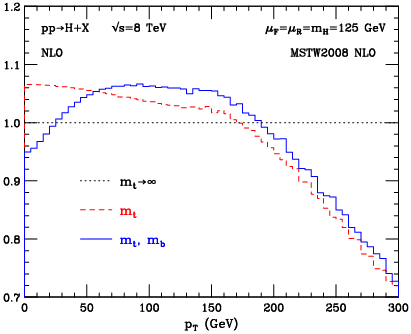
\includegraphics[width=0.5\textwidth]{images/pth_quarkmass.png}
\caption{\pth distribution computed at NLO ($\alpha_s^3$) and normalized to the calculation obtained in the large-$m_\mathrm{t}$ approximation. The red dashed line corresponds to the calculation including the top quark mass while the blue line refers to the calculation including also the bottom quark effects.}\label{fig:pth_quarkmass}
\end{figure}

Possible extensions of the SM predict a modification of the Higgs boson couplings to gluons and to the top quark. Many of these models actually predict the existence of new states that interact with the SM Higgs boson, but are beyond the direct production reach at the actual LHC energies. The effect of these new states could however show up as a deviation of the Higgs boson couplings with respect to the SM expectation. The modification of the couplings, as shown in Refs.~\cite{Azatov:2013xha,Harlander:2013oja}, can change the kinematics of the Higgs boson production and the effect can be particularly sizeable in the tail of the \pth distribution. 
Other models, such as Composite Higgs~\cite{Marzocca:2012zn}, predict the existence of top-partners, which are heavy resonances with the same quantum numbers as the top quark, that can interact with the Higgs boson in the ggH fermionic loop, changing the \pth shape with respect to what the SM predicts~\cite{Banfi:2013yoa}.
The measurement of the \pth spectrum is thus a useful tool for indirect searches of new particles predicted by theories beyond the SM.

Measurements of the fiducial cross sections and of several differential
distributions, using the $\sqrt{s}=8$\TeV LHC data, have been reported by ATLAS~\cite{Aad:2014tca,Aad:2014lwa,Aad:2015lha} and CMS~\cite{Khachatryan:2015rxa,Khachatryan:2015yvw} for the ${\mathrm{H} \to \mathrm{ZZ} \to 4\ell}$ ($\ell = \mathrm{e},\mu$) and H $\to \gamma\gamma$ decay channels. In this chapter a measurement of the fiducial cross section times branching fraction ($\sigma \times \mathcal{B}$) and \pt{} spectrum for Higgs boson production in \ensuremath{\mathrm{H}\rightarrow{}\WW\rightarrow \mathrm{e}^{\pm} \mu^{\mp}\nu\nu} ~decays, based on $\sqrt{s} = 8$\TeV LHC data, is reported.

The analysis is performed looking at different flavour leptons in the final state in order to suppress the sizeable contribution of backgrounds containing a same-flavour lepton pair originating from Z boson decay.

Although the \hwwllnn{} channel has lower resolution in the \pth{} measurement
compared to the H $\to \gamma\gamma$ and  H $\to \rm{ZZ}\to 4\ell$ channels
because of neutrinos in the final state, the channel has a significantly
larger $\sigma \times \mathcal{B}$, exceeding those for H $\to \gamma\gamma$ by a factor
of 10 and H $\to \rm{ZZ}\to 4\ell$ by a factor of 85 for a Higgs boson mass of
125\GeV~\cite{Heinemeyer:2013tqa}, and is characterized by good signal
sensitivity. Such sensitivity allowed the observation of a Higgs boson at the level of 4.3 (5.8 expected)
standard deviations for a mass hypothesis of 125.6 GeV using the full LHC data set at 7 and 8\TeV~\cite{Chatrchyan:2013iaa}.

The measurement is performed in a fiducial phase space defined by kinematic requirements on
the leptons that closely match the experimental event selection.

The effect of the limited detector resolution, as well as the
selection efficiency with respect to the fiducial phase space are corrected to
particle level with an unfolding procedure~\cite{Cowan:2002in}, as explained in Sec.~\ref{sec:Unfolding}.



\cleardoublepage
\chapter{Physics at the LHC}\label{chap1}
\thispagestyle{empty}

In this chapter the Standard Model (SM) of particle physics is briefly described, in particular the main characteristics of the electroweak and strong interactions are discussed, as well as the mechanism of the electroweak symmetry breaking. Afterwards, few models that provide a simple extension of the SM Higgs sector are illustrated.
In addition, the phenomenology of Higgs boson production at LHC is described, focusing on its kinematic properties and, in particular, on the \hww decay channel. An overview of the main features of the Monte Carlo (MC) simulation techniques for the Higgs boson production is also given, as well as a brief report of the Higgs boson highlights from the experiments.

\noindent Unless otherwise stated, natural units $\hslash=c=1$ are used throughout this work.

\section{The Standard Model of particle physics}
%%%%%%%%%%%%%%%%%%%%%%%%%%%%%%%%%%%%%%%%%%%%%%%%%%%%%%%%%%%%%%%%%%%%%%
\label{sec:SM}

The Standard Model of Particle Physics is the theory that describes all fundamental constituents of matter and their interactions~\cite{Halzen:1984mc}. It is a renormalisable quantum field theory based on a $\mathrm{SU(3)_c \otimes SU(2)_L \otimes U(1)_Y}$ local gauge symmetry, and is capable to provide a quantitative description of three of the four interactions in nature: electromagnetism, weak interaction and strong nuclear force. 

According to the SM, the ordinary matter is made up of spin-$1/2$ particles, denoted as fermions. The fermions are subdivided into two classifications of elementary particles: leptons and quarks. Both classes consist of six particles, grouped into three doublets, called generations. Additional three doublets for each class are composed of leptons and quarks antiparticles. A charged particle with electric charge $Q=-1$, either the electron e, the muon $\mu$ or the tauon $\tau$, and a neutral particle, the corresponding neutrino, compose the following lepton generations, ordered according to an increasing mass hierarchy:

\begin{equation}
\label{eq:leptons}
\begin{pmatrix} \rm e^-       \\ \nu_{\rm e}      \end{pmatrix}, \quad
\begin{pmatrix} \mu^-     \\ \nu_{\mu}  \end{pmatrix}, \quad
\begin{pmatrix} \tau^-    \\ \nu_{\tau} \end{pmatrix}  \quad .
\end{equation}

Charged leptons can interact via the electromagnetic and weak force, while neutrinos, that are assumed to be massless, can interact only through the weak interaction.

Similarly, the quarks are organized in pairs composed of a particle with $Q=+2/3$, \emph{up} (u), \emph{charm} (c) and \emph{top} (t) quarks, and another particle with $Q=-1/3$, \emph{down} (d), \emph{strange} (s) and \emph{bottom} (b) quarks:

\begin{equation}
\label{eq:quarks}
\begin{pmatrix} \rm u       \\ \rm d      \end{pmatrix}, \quad
\begin{pmatrix} \rm c       \\ \rm s      \end{pmatrix}, \quad
\begin{pmatrix} \rm t       \\ \rm b      \end{pmatrix}  \quad .
\end{equation}

As well as leptons, quarks can interact via the electromagnetic and weak force, but also through the strong interaction, responsible of their confinement within hadrons. In fact, free quarks are not observed in nature, but they bind together forming two categories of hadrons: mesons, bound states of a quark q and an anti-quark $\mathrm{\bar{q}}$, and baryons, bound states of three quarks.

In the SM the interaction between elementary particles occurs through the exchange of spin-1 particles, known as bosons, which identify the fundamental forces. The photon $\gamma$ is the mediator of the electromagnetic interaction, the $\mathrm{W^{\pm}}$ and Z bosons are the mediators of the weak interaction, while the strong force is mediated by eight gluons g. Electromagnetic and weak interactions are actually the manifestations of the same fundamental interaction, the electroweak force.


%%% EWK
\subsection{The electroweak interaction}

The theory of electroweak interaction was formulated in the 1960s by S. L. Glashow, A. Salam and S. Weinberg~\cite{Glashow:1961tr,Weinberg:1967tq} as an $\mathrm{SU(2) \otimes U(1)}$ local gauge theory.
The Lagrangian density governing the electroweak interaction is therefore invariant under gauge transformations of the $\mathrm{SU(2)_L\otimes U(1)_Y}$ symmetry group. The $\mathrm{SU(2)_L}$ group refers to the weak isospin charge $I$, while $\mathrm{U(1)_Y}$ to the weak hypercharge $Y$, which are connected to the charge Q by the following equation:

\begin{equation}
Y = 2(Q - I_3) \quad,
\end{equation}

\noindent where $I_3$ represents the third component of the weak isospin. 

According to the Noether theorem, the $\mathrm{SU(2)_L}$ invariance of the theory leads to the existence of three conserved currents, $J_\mu^\pm$ and $J_\mu^3$, which constitute an isospin triplet of weak currents. 
The two currents $J_\mu^\pm$ represent the weak charged current interactions, which describe the interaction between fermions that are mediated by the charged $\mathrm{W^\pm}$ bosons. These currents only involve left-handed particles or right-handed anti-particles, in accordance with the fact that the parity symmetry is maximally violated for weak charged current interactions, as confirmed by the experiments of Madame Wu~\cite{Wu:1957my} and Garwin-Lederman-Weinrich~\cite{Garwin:1957hc} in 1957. In the case of leptons, charged currents can only connect two particles within the same generation, for example the electron and the electron neutrino, while for the quarks a mixing of different generations may occur, according to the Cabibbo-Kobayashi-Maskawa matrix (CKM).

Another possible interaction in the weak sector is known as neutral current interaction and is mediated by the neutral Z boson. In the vertex of this interaction the identity of the interacting lepton does not change, resembling in this matter the electromagnetic current. Concerning the quark sector, the weak neutral currents involving different quark flavours, i.e. \emph{flavour changing neutral currents}, are strictly suppressed at tree level by the Glashow-Iliopoulos-Maiani mechanism (GIM)~\cite{Glashow:1970gm}.

Nevertheless, the other component of the weak isospin triplet of currents $J_\mu^3$, cannot be identified with the weak neutral current, because the weak neutral current involves both left- and right-handed components. The electromagnetic current cannot be represented by $J_\mu^3$ as well, for the aforementioned reason and because it cannot be coupled with the uncharged neutrino. In order to save the $\mathrm{SU(2)}$ symmetry, the existence of the $\mathrm{U(1)_Y}$ symmetry is required, and a new conserved current, $j_\mu^Y$, arises. The $j_\mu^Y$ current is unchanged under $\mathrm{SU(2)}_L$ transformations (is an isospin singlet) and is incorporated, together with $J_\mu^3$, in the definition of the electromagnetic current, giving rise to the electroweak unification.

Local gauge symmetries naturally lead to the presence of gauge bosons, the exchange particles mediators of the fundamental interactions. The symmetry requires these gauge bosons to be massless, which is unproblematic for photons and gluons, but in drastic contrast to the known masses of the Z and $\mathrm{W^\pm}$ bosons, which are $m_\mathrm{Z} = 91.1876 \pm 0.0021$\GeV and $m_\mathrm{W} = 80.385 \pm 0.015$\GeV, respectively. Moreover, the maximally parity violating structure of the weak charged currents also breaks local gauge invariance for all massive fermions, due to their coupling to the W boson. This leads to the apparent antagonism that, while the $\mathrm{SU(2)_L \otimes U(1)_Y}$ gauge symmetry does describe the coupling structure of the electroweak force, at the same time it seems to contradict the fact that the W and Z bosons, and all fermions have a non-vanishing mass. 

The proposed solution to this problem is the mechanism of \emph{spontaneous symmetry breaking}, where the gauge symmetry is still intrinsic to the Lagrangian density of the theory, but not manifest in its energy ground state, which in this case is the quantum vacuum. The spontaneous symmetry breaking of the $\mathrm{SU(2)_L \otimes U(1)_Y}$ symmetry group requires the introduction of a self-interacting complex scalar field~\cite{Wolf:2015kua}, which is an isospin doublet:
\begin{equation}
\phi = \begin{pmatrix} \phi^+       \\ \phi^0      \end{pmatrix} = \begin{pmatrix} (\phi_1+i\phi_2)/\sqrt{2}       \\ (\phi_3+i\phi_4)/\sqrt{2}      \end{pmatrix} \quad .
\end{equation}

\noindent The simplest lagrangian involving this field has the form:
\begin{equation}\label{eq:higgsL}
\begin{split}
\mathcal{L}_\mathrm{H} &= \mathcal{D}_\mu \phi^\dagger \mathcal{D}^\mu \phi - V(\phi) \quad,\\
V(\phi) &= -\mu^2\phi^\dagger\phi + \lambda(\phi^\dagger\phi)^2
\end{split}
\end{equation}

\noindent Here th $\mathcal{D}_\mu$ represents the covariant derivative defined as:
\begin{equation}
\mathcal{D}_\mu = \partial_\mu + i g \vec{A}_\mu \cdot \frac{\vec{\tau}}{2} - \frac{1}{2}i g' Y B_\mu \quad ,
\end{equation}
\noindent where $\vec{A}_\mu$ is a vector of three gauge fields satisfying the local $\mathrm{SU(2)}$ symmetry, and $B_\mu$ is the gauge field assuring the $\mathrm{U(1)}$ symmetry. The parameters $g$ and $g'$ represent the coupling constants for the gauge fields.

The term $V(\phi)$ in Eq.\eqref{eq:higgsL} is a potential term that depends on two parameters, $\mu$ and $\lambda$, with $\lambda>0$ in order to have vacuum stability. If the $\mu$ parameter is chosen so that $\mu^2<0$, the symmetry of $V(\phi)$ may be broken, since its minimum value is degenerate:
\begin{equation}
\phi^\dagger\phi = -\frac{\mu^2}{2\lambda} = \frac{v^2}{2} \quad ,
\end{equation}

\noindent where $v$ corresponds to the \emph{vacuum expectation value} (VEV). Perturbation theory requires an expansion of $\phi$ around its energy ground state. The ground state is chosen in such a way it  breaks the $\mathrm{SU(2)_L \otimes U(1)_Y}$ symmetry group but preserves the invariance under $\mathrm{U(1)_{em}}$ transformations, i.e. it has a null electric charge. This latter requirement guarantees the presence of a neutral massless gauge boson, the photon. Therefore, the ground state can be written without any loss of generality as:
\begin{equation}
\tilde{\phi} = \frac{1}{\sqrt{2}} \begin{pmatrix} 0 \\ v   \end{pmatrix}\quad .
\end{equation}
The field $\phi$ can be expanded at first order around the ground state obtaining:
\begin{equation}
\phi = \frac{1}{\sqrt{2}} \begin{pmatrix} 0 \\ v+h   \end{pmatrix}\quad .
\end{equation}
Introducing this field in the Higgs Lagrangian in Eq.~\eqref{eq:higgsL}, the bosonic fields acquire a mass given by:
\begin{equation}
m_\mathrm{W} = \frac{v}{2}g \qquad m_\mathrm{Z} = \frac{v}{2}\sqrt{g^2 +g'^2} \quad,
\end{equation}
\noindent where $g$ and $g'$ are the electroweak coupling constants for the gauge fields.

Furthermore, given the self-interaction terms of the $h$ field, a new physical state also arises (the Higgs boson) with a mass:
\begin{equation}
m_\mathrm{H} = v\sqrt{2\lambda} \quad.
\end{equation}
\noindent whose value is not predicted by the theory, since $\lambda$ is unknown\footnote{On the other hand, the value of $v$ can be obtained using the relation between $m_\mathrm{W}$ and the Fermi constant $G_\mathrm{F}$, which leads to $v = 1/\sqrt{\sqrt{2}G_\mathrm{F}} = 246.22$\GeV, setting the scale of the electroweak symmetry breaking.}.

The mass of fermions is achieved without breaking the gauge symmetry of the Lagrangian by introducing a coupling term, known as Yukawa coupling, between the fermion doublets and the Higgs field.

In addition to the mass of the particles, the model also predicts the couplings $f$ of the Higgs boson to fermions and heavy gauge bosons, despite their numerical values need to be determined by experiments:
\begin{equation}
\begin{split}
f_\mathrm{H\to ff} &\propto \frac{m_\mathrm{f}}{v} ,\quad \text{fermions}\\
f_\mathrm{H\to VV} &\propto \frac{2m_\mathrm{V}^2}{v} ,\quad \text{heavy bosons trilinear}\\
f_\mathrm{HH\to VV} &\propto \frac{2m_\mathrm{V}^2}{v^2} ,\quad \text{heavy bosons quartic}\\
f_\mathrm{H\to HH} &\propto \frac{3m_\mathrm{H}^2}{v} ,\quad \text{Higgs boson trilinear}\\
f_\mathrm{HH\to HH} &\propto \frac{3m_\mathrm{H}^2}{v^2} ,\quad \text{Higgs boson quartic} \quad .
\end{split}
\end{equation}

During the past decades the predictions of the SM have been confirmed by experimental results with outstanding precision, and in 2012 the discovery of a new boson with a mass of about 125\GeV, consistent with the predicted Higgs boson, was announced by the ATLAS and CMS experiments at LHC.


\subsection{The strong interaction}

Quantum Chromo-Dynamics (QCD) is the theory that describes the strong interactions~\cite{Ellis:1991qj}. It is an unbroken gauge non-abelian theory based on the group $\mathrm{SU(3)}$ of colour ($\mathrm{SU(3)_c}$). The mediators of the interaction are eight massless gluons and the elementary particles of matter are colour triplets of quarks, with different flavours. In fact, as shown in \eqref{eq:quarks}, six types (flavours) of quark exist and each quark possesses a colour charge that can assume three values, namely red, green and blue.

The physical vertices in QCD include the gluon-quark-antiquark vertex, analogous to the Quantum Electro-Dynamics (QED) photon-fermion-antifermion coupling, but also the three-gluon and four-gluon vertices, i.e. gluon themselves carry colour charge, which have no analogue in an abelian theory like QED. Quark and gluons are the only particles that interact through the strong interaction.

The non-abelian nature of the theory leads to two important characteristics:
\begin{itemize}
\item \emph{colour confinement}: the QCD coupling constant $\alpha_s = g_s^2/4\pi$ is a function of the scale of the interaction $Q$. At low energy (corresponding to large distances of the order of 1\,fm) the $\alpha_s$ value is large and a perturbative approach is not applicable. When a quark-antiquark pair begins to separate, the colour field generated by the exchanged gluons increases its intensity and, at some point, the creation of a new quark-antiquark pair from the vacuum becomes more energetically favourable than increasing further the interaction strength. This explains why free quarks are not observed and the final state particles are made of colourless quark bound states (hadrons). This is also the cause of the hadronization process which causes the formation of jets.

\item \emph{asymptotic freedom}: the coupling constant decreases at large scales $Q$ approaching to zero, meaning that quarks can be asymptotically considered as free particles. The small value of the coupling constant at large scales justifies the usage of a perturbative approach to describe hard processes.
\end{itemize}


%\section{Electroweak interaction}
%%%%%%%%%%%%%%%%%%%%%%%%%%%%%%%%%%%%%%%%%%%%%%%%%%%%%%%%%%%%%%%%%%%%%%
\label{sec:EW}

The theory of electroweak interaction was formulated in the 1960s by S. L. Glashow, A. Salam and S. Weinberg~\cite{Glashow:1961tr,Weinberg:1967tq} as an $\mathrm{SU(2) \otimes U(1)}$ local gauge theory.
In 1957 the experiments lead by Madame Wu~\cite{Wu:1957my} and Garwin-Lederman-Weinrich~\cite{Garwin:1957hc} confirmed that the parity symmetry is maximally violated for weak charged current interactions, proving that only left-handed particles or right-handed antiparticles are involved in these interactions. 

To express this aspect the weak charged currents can be written making use of the Dirac spinors, $\ell$ and $\nu_\ell$ (representing the lepton and neutrino spinors, repsectively), as follows:

\begin{equation}
\begin{split}
J_\mu^+ &= \bar{\nu}_\ell \gamma_\mu \dfrac{1}{2}(1-\gamma^5) \ell \quad, \\
J_\mu^- &= \bar{\ell} \gamma_\mu \dfrac{1}{2}(1-\gamma^5)\nu_\ell \quad,
\end{split}
\end{equation}

where the ``$+$'' and ``$-$'' superscripts indicate the charge-raising and charge-lowering character of the currents, and $\gamma^5 = i\gamma^0\gamma^1\gamma^2\gamma^3$ is the product of the Dirac $\gamma$ matrices. In fact, the effect of the projector $P=\dfrac{1}{2}(1-\gamma^5)$ is to project the spinor to its left-handed component. Therefore, introducing the following doublet:

\begin{equation}
\chi_L = \begin{pmatrix} \nu_\ell \\ \ell \end{pmatrix}_L \quad ,
\end{equation}

where $L$ denotes the left-handed component of the spinor, and defining the ``step-up'' and ``step-down'' operators $\tau_\pm = \dfrac{1}{2}(\tau_1 \pm i\tau_2)$, where $\tau_i$ are the Puali matrices, the charged currents become:

\begin{equation}
\begin{split}
J_\mu^+ &= \bar{\chi}_L \gamma_\mu \tau_+ \chi_L \quad, \\
J_\mu^- &= \bar{\chi}_L \gamma_\mu \tau_- \chi_L \quad.
\end{split}
\end{equation}

In order to complete the $\mathrm{SU(2)}$ invariance of the theory, a third conserved current should exist with the form:

\begin{equation}
J_\mu^3 = bar{\chi}_L \gamma_\mu \dfrac{1}{2} \tau_3 \chi_L = \dfrac{1}{2}\bar{\nu}_L \gamma_\mu \nu_L -  \dfrac{1}{2}\bar{\ell}_L \gamma_\mu \ell_L \quad,
\end{equation}

The three currents $J_\mu^\pm$ and $J_\mu^3$ constitute an isospin triplet of weak currents, with corresponding charges

\begin{equation}
T^i = \int J_0^i(x)d^3x \quad,
\end{equation}

that generate the $\mathrm{SU(2)}_L$ algebra defined by the following rules:

\begin{equation}
\left[T^i, T^j \right] = i \varepsilon_{ijk} T^k \quad.
\end{equation}

Nevertheless, $J_\mu^3$ cannot be identified with the weak neutral current, because the weak neutral current involves both left- and right-handed components. The electromagnetic current cannot be represented by $J_\mu^3$ as well, for the aforementioned reasons and because it cannot be coupled with the uncharged neutrino.

In order to save the $\mathrm{SU(2)}$ symmetry, the existence of a new $\mathrm{U(1)}$ symmetry is required, and a new conserved current arises. The new symmetry is known as hypercharge symmetry ($\mathrm{U(1)_Y}$) and the corresponding conserved current is:

\begin{equation}
j_\mu^Y = \bar{\psi} \gamma_\mu Y \psi \quad,
\end{equation}

where $\psi$ is a generic Dirac spinor and the hypercharge $Y$ is defined as:

\begin{equation}
Y = 2(Q - T_3)
\end{equation}

The $j_\mu^Y$ current is unchanged under $\mathrm{SU(2)}_L$ transformations (is an isospin singlet). The electromagnetic and weak interactions can be incorporated defining the electromagnetic current as:

\begin{equation}
j_\mu^{em} = J_\mu^3 + \dfrac{1}{2} j_\mu^Y \quad,
\end{equation}

which represents the electroweak unification. 
\begin{comment}
Also, the weak neutral current $J_\mu^{NC}$ can be written as a combination of $J_\mu^3$ and $j_\mu^{em}$ as follows:

\begin{equation}
J_\mu^{NC} = J_\mu^3 - \sin ^2 \theta_W j_\mu^{em} \quad,
\end{equation}

where $\theta_W$ is the Weinberg angle.
\end{comment}
The electroweak lagrangian can be expressed in a local $\mathrm{SU(2)}_L \otimes \mathrm{U(1)}_Y$ gauge invariant form by introducing the covariant derivatives $\mathcal{D}_\mu$ in place of the ordinary derivatives:

\begin{equation}
\mathcal{D}_\mu = \partial_\mu + i g \vec{A}_\mu \cdot \frac{\vec{\tau}}{2} - \frac{1}{2}i g' Y B_\mu \quad ,
\end{equation}

where $\vec{A}_\mu$ is a vector of three gauge fields satisfying the local $\mathrm{SU(2)}$ symmetry, and $B_\mu$ is the gauge field assuring the $\mathrm{U(1)}$ symmetry. The parameters $g$ and $g'$ represent the coupling constants for the gauge fields. The electroweak lagrangian can thus be written as:

\begin{equation}
\mathcal{L} = \sum_{f} \bar{\psi}i\gamma_\mu\mathcal{D}_\mu\psi = \sum_{f} \bar{\psi}i\gamma_\mu\partial_\mu\psi + \mathcal{L}_int \quad,
\end{equation}

where $\mathcal{L}_int$ represents the interaction terms.

%\section{The Higgs mechanism}
%%%%%%%%%%%%%%%%%%%%%%%%%%%%%%%%%%%%%%%%%%%%%%%%%%%%%%%%%%%%%%%%%%%%%%
\label{sec:Higgs}

Local gauge symmetries naturally lead to the presence of gauge bosons, the exchange particles mediators of the fundamental interactions. The symmetry requires these gauge bosons to be massless, which is unproblematic for photons and gluons, but in drastic contrast to the known masses of the Z and $\mathrm{W^\pm}$ bosons, which are $m_\mathrm{Z} = 91.1876 \pm 0.0021$\GeV and $m_\mathrm{W} = 80.385 \pm 0.015$\GeV, respectively. Moreover, the maximally parity violating structure of the weak charged currents also breaks local gauge invariance for all massive fermions, due to their coupling to the W boson. This leads to the apparent antagonism that, while the $\mathrm{SU(2)_L \otimes U(1)_Y$ gauge symmetry does describe the coupling structure of the electroweak force, at the same time it seems to contradict the fact that the W and Z bosons, and all fermions have a non-vanishing mass. 

The proposed solution to this problem is the mechanism of spontaneous symmetry breaking, where the gauge symmetry is still intrinsic to the Lagrangian density of the theory, but not manifest in its energy ground state, which in this case is the quantum vacuum.

%\section{The strong interaction}
%%%%%%%%%%%%%%%%%%%%%%%%%%%%%%%%%%%%%%%%%%%%%%%%%%%%%%%%%%%%%%%%%%%%%%
\label{sec:QCD}


\section{Beyond the Standard Model}
%%%%%%%%%%%%%%%%%%%%%%%%%%%%%%%%%%%%%%%%%%%%%%%%%%%%%%%%%%%%%%%%%%%%%%
\label{sec:BSM}

The discovery of the new boson in accordance with the Higgs boson predicted by the SM has been a major breakthrough in the contemporary particle physics. The Higgs boson mass is a free parameter in the SM and its measurement fixes all the other parameters related to the Higgs field, such as the coupling strengths with bosons and fermions. The current quest is to establish whether the properties of the discovered boson are consistent with the SM predictions, or it is only a component of a more entangled Higgs sector. Moreover, there are still several aspects that are not explained by the SM, such as the hierarchy problem, the nature of dark matter and others~\cite{Langacker:2010zza}.

Several theoretical models have been proposed to explain the deficiencies of the SM. One of the simplest extension of the SM Higgs sector requires the existence of an additional singlet scalar field, S, which is neutral under all quantum numbers of the SM gauge group~\cite{Robens:2015gla}. In general the singlet field mixes with the SM Higgs boson, H, allowing it to couple to the same states as the SM Higgs boson itself. If the mass of the scalar singlet was more than twice that of the SM Higgs boson, the S branching ratios would be reduced with respect to the H ones, because of the opening of the new $\mathrm{S \to HH}$ decay channel.

The mixing of the two states S and H would manifest as a suppression of the production cross section of both states and a suppression of the heavy mass Higgs boson decay modes to SM particles, if the $\mathrm{S \to HH}$ decay is kinematically accessible. In particular, identifying as H the observed Higgs boson with $m_\mathrm{H} = 125$\GeV, and supposing that the new scalar singlet S is heavier than H, one can introduce the scale factors of the low and high mass state couplings, $\mathcal{C}$ and $\mathcal{C'}$, respectively. These factors are related by the unitarity condition $\mathcal{C}^2 + \mathcal{C'}^2 = 1$. The singlet cross section and width are consequently modified by the factors $\mu'$ and $\Gamma'$, respectively:

\begin{equation}
\begin{split}
\mu' &= \mathcal{C'}^2 \cdot (1 - \mathcal{B}_\mathrm{new}) \quad ,\\
\Gamma' &= \Gamma_\mathrm{SM} \cdot \frac{\mathcal{C'}^2}{1 - \mathcal{B}_\mathrm{new}} \quad ,
\end{split}
\end{equation}

\noindent where $\mathcal{B}_\mathrm{new}$ is the singlet branching fraction to non-SM-like decay modes.

Other models, such as the \emph{two-Higgs-doublet model} (2HDM)~\cite{Branco:2011iw}, extend the minimal Higgs content requiring the introduction of a second Higgs doublet. 
The generalization of the SM Lagrangian with two complex scalar fields, which are $\mathrm{SU(2)_L}$ doublets, eventually gives rise to five physical Higgs bosons: a charged pair ($H^{\pm}$); two neutral $CP$-even scalars (H and h, where $m_{\rm H}>m_{\rm h}$ by convention); and a neutral $CP$-odd scalar (A)~\cite{Craig:2013hca}. The parameter space of these 2HDM models can accommodate a wide range of variations in the production and decay modes of the SM-like Higgs boson. Nevertheless, tight constraints on flavour-changing neutral currents disfavour 2HDM with tree-level flavour violation. Similarly, limits on additional sources of $CP$ violation favour 2HDM with a $CP$-conserving potential. These assumptions significantly reduce the parameter space of 2HDM models. Moreover, if the h boson is identified with the observed 125\GeV boson, the experimental measurements further constraint the possible production and decay modes of the other predicted particles. Examples of possible decay channels in this framework are the following: the  heavy  $CP$-even  Higgs  may  decay  to  two  light  CP-even  Higgs, $\mathrm{H \to hh}$; the $CP$-odd pseudoscalar Higgs may decay to a light $CP$-even Higgs and a Z boson, $\mathrm{A \to Zh}$; the charged Higgs bosons may decay to a SM-like Higgs and a $\mathrm{W}^\pm$ boson, $\mathrm{H^\pm \to \mathrm{W}^\pm h}$.

In order to search for new particles that could be ascribable to the simple models depicted above, or even to more complicated theories, it is of utmost importance to provide precise measurements of the Higgs boson couplings and kinematics, as well as its spin and parity properties. A complementary strategy is to perform direct searches for additional Higgs bosons in the full mass range accessible to current and future experiments.

\section{Phenomenology of proton proton interactions}
%%%%%%%%%%%%%%%%%%%%%%%%%%%%%%%%%%%%%%%%%%%%%%%%%%%%%%%%%%%%%%%%%%%%%%
\label{sec:ppInt}


\section{Higgs boson phenomenology}
%%%%%%%%%%%%%%%%%%%%%%%%%%%%%%%%%%%%%%%%%%%%%%%%%%%%%%%%%%%%%%%%%%%%%%
\label{sec:HiggsPheno}

In this section the Higgs boson production modes and decay channels are described, spending some time on the description of the \hww channel, which is the channel investigated in this work. Afterwards, a description of the effects due to higher order QCD corrections on Higgs boson kinematic variables is shown. Finally, a brief review of the Monte Carlo (MC) generators used for the simulation of Higgs boson processes is given.

%One of the main goals of the LHC was the search for the SM Higgs boson over a wide range of masses. This goal has been achieved in 2012, when the ATLAS and CMS collaborations announced the discovery of a new boson with mass $m_\mathrm{H} = 125$\GeV~\cite{Aad:2012tfa,Chatrchyan:2012xdj}, consistent with the SM Higgs boson prediction.




%%%%%%%%%%%%%%%%%%%%%%%%%%%%%%%%%%%%%%%%%%%%%%%%%%%%%%%%%%%%%%%%%%%%%%
\subsection{Higgs boson production mechanisms and decay channels}

The main processes contributing to the Higgs boson production at hadron colliders are represented by the Feynman diagrams shown in Fig.~\ref{fig:higgs_prod}.

\begin{figure}[htb]
\centering
\subfigure[ggH]{
 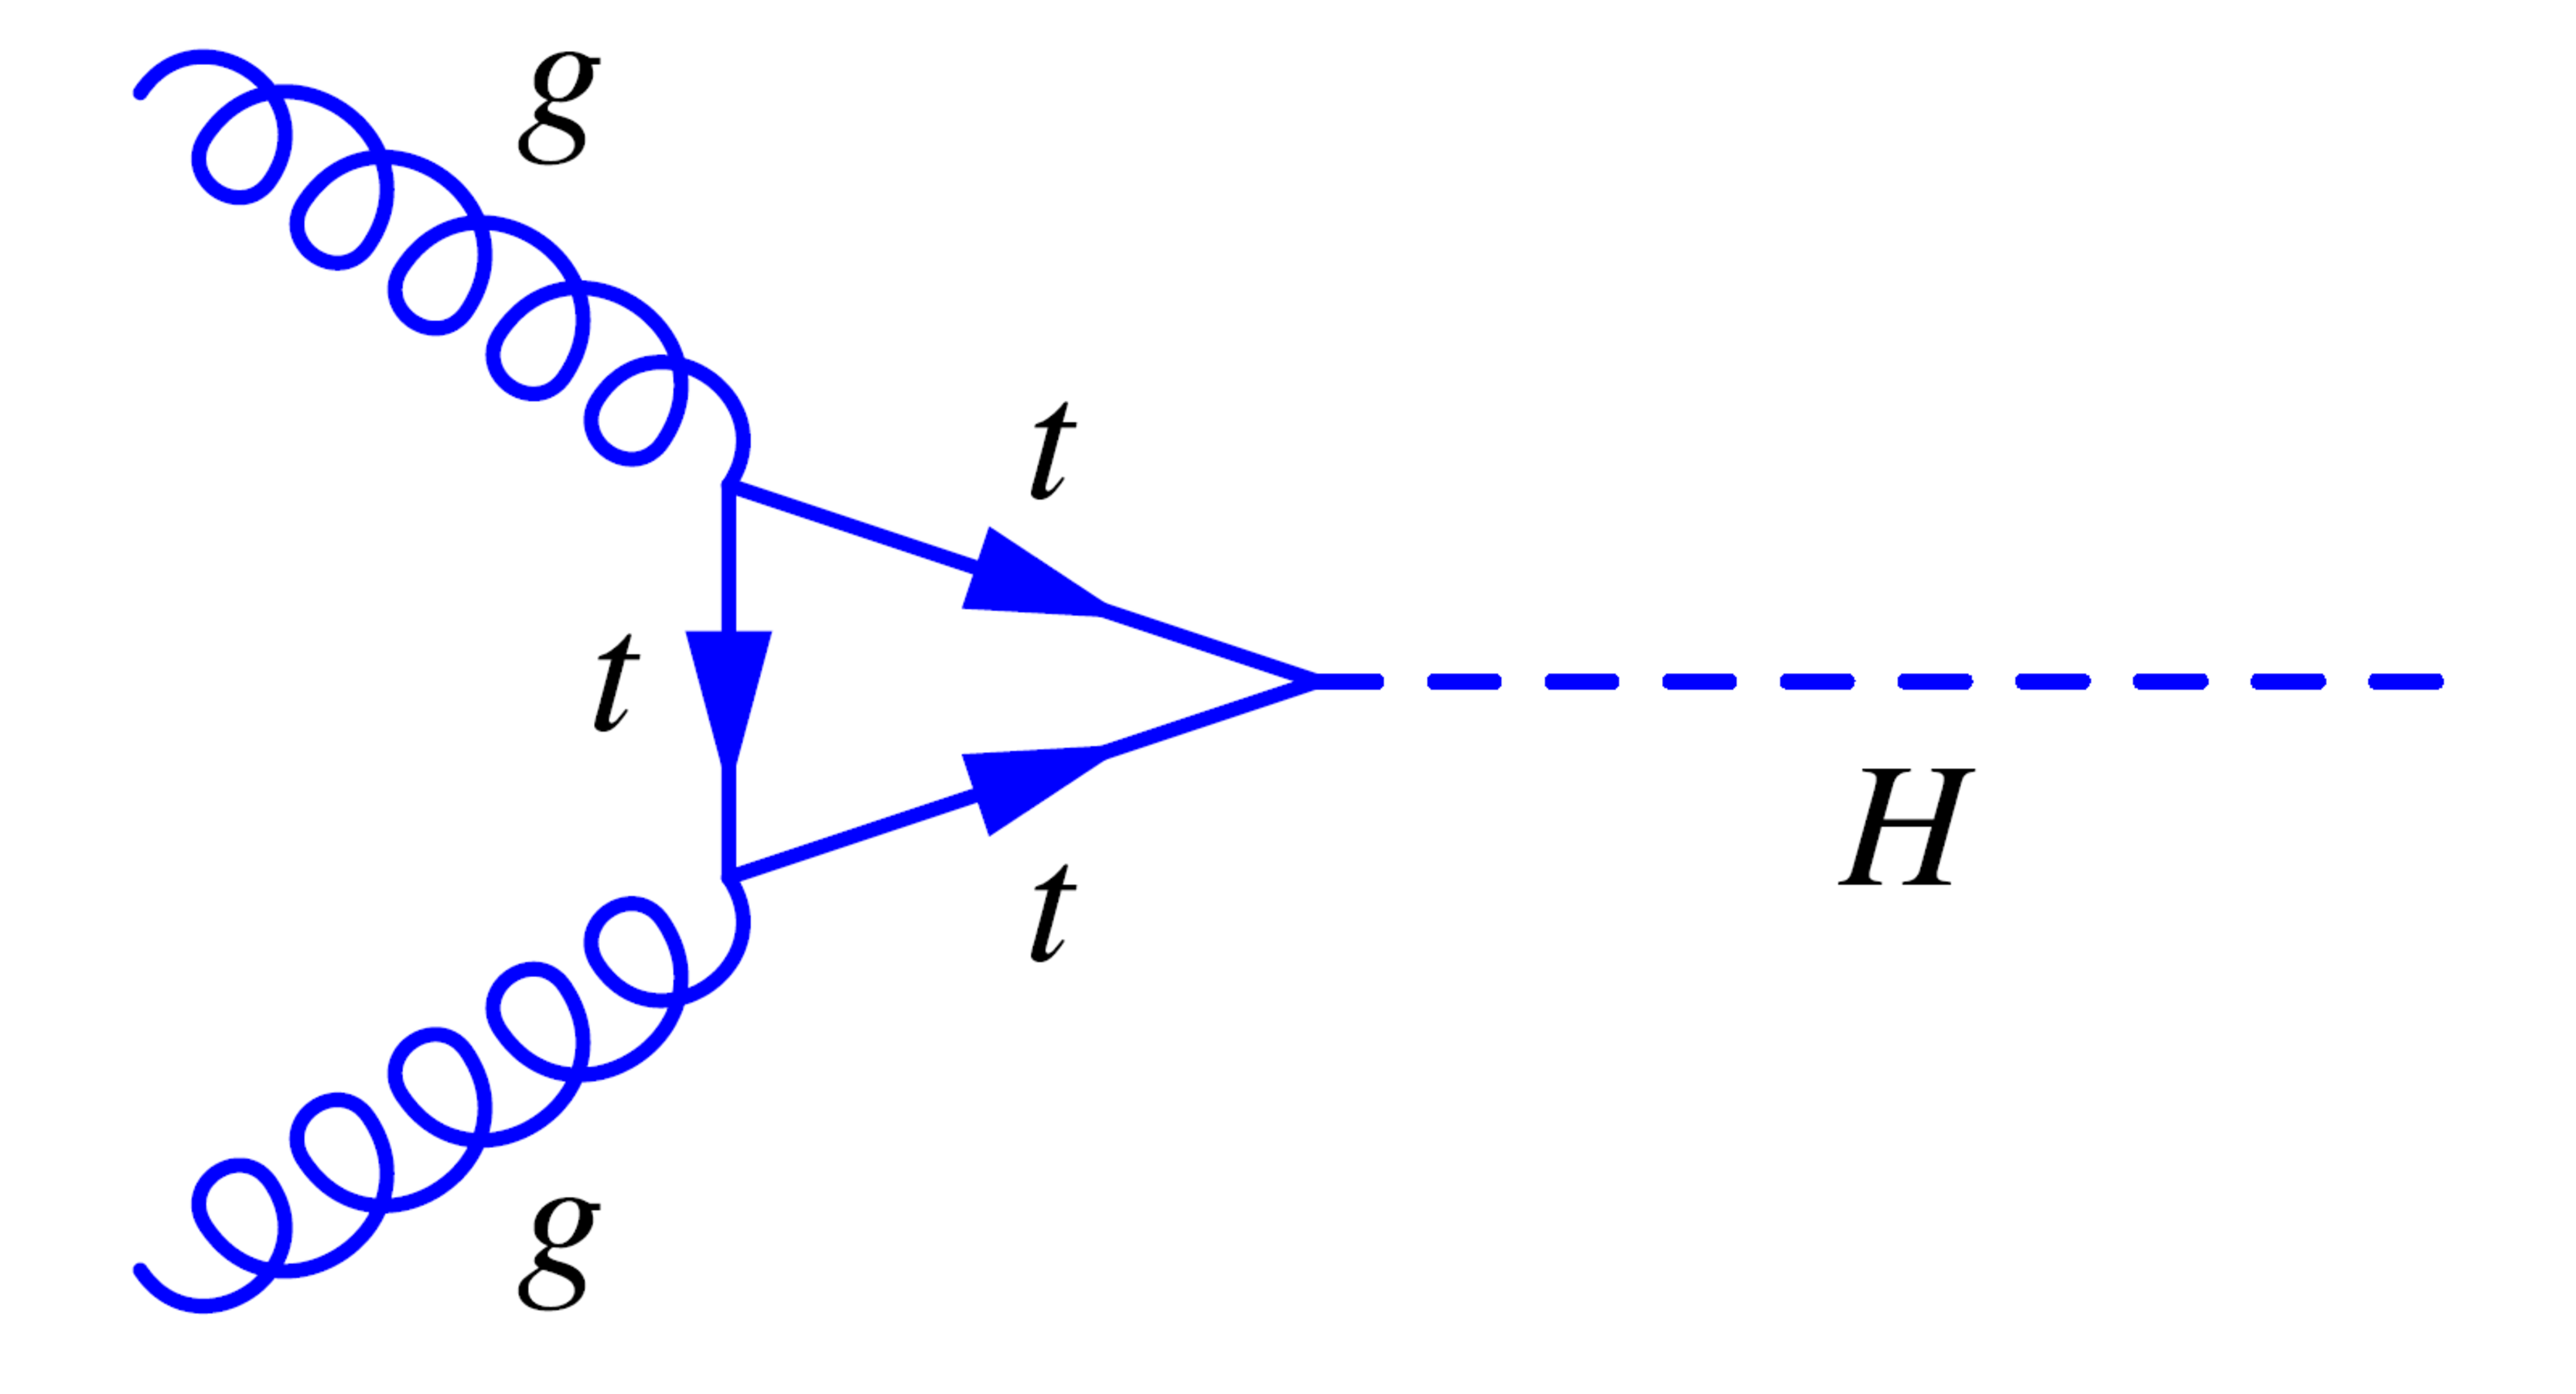
\includegraphics[width=0.45\textwidth]{images/ggH.pdf}
}
\subfigure[VBF]{
 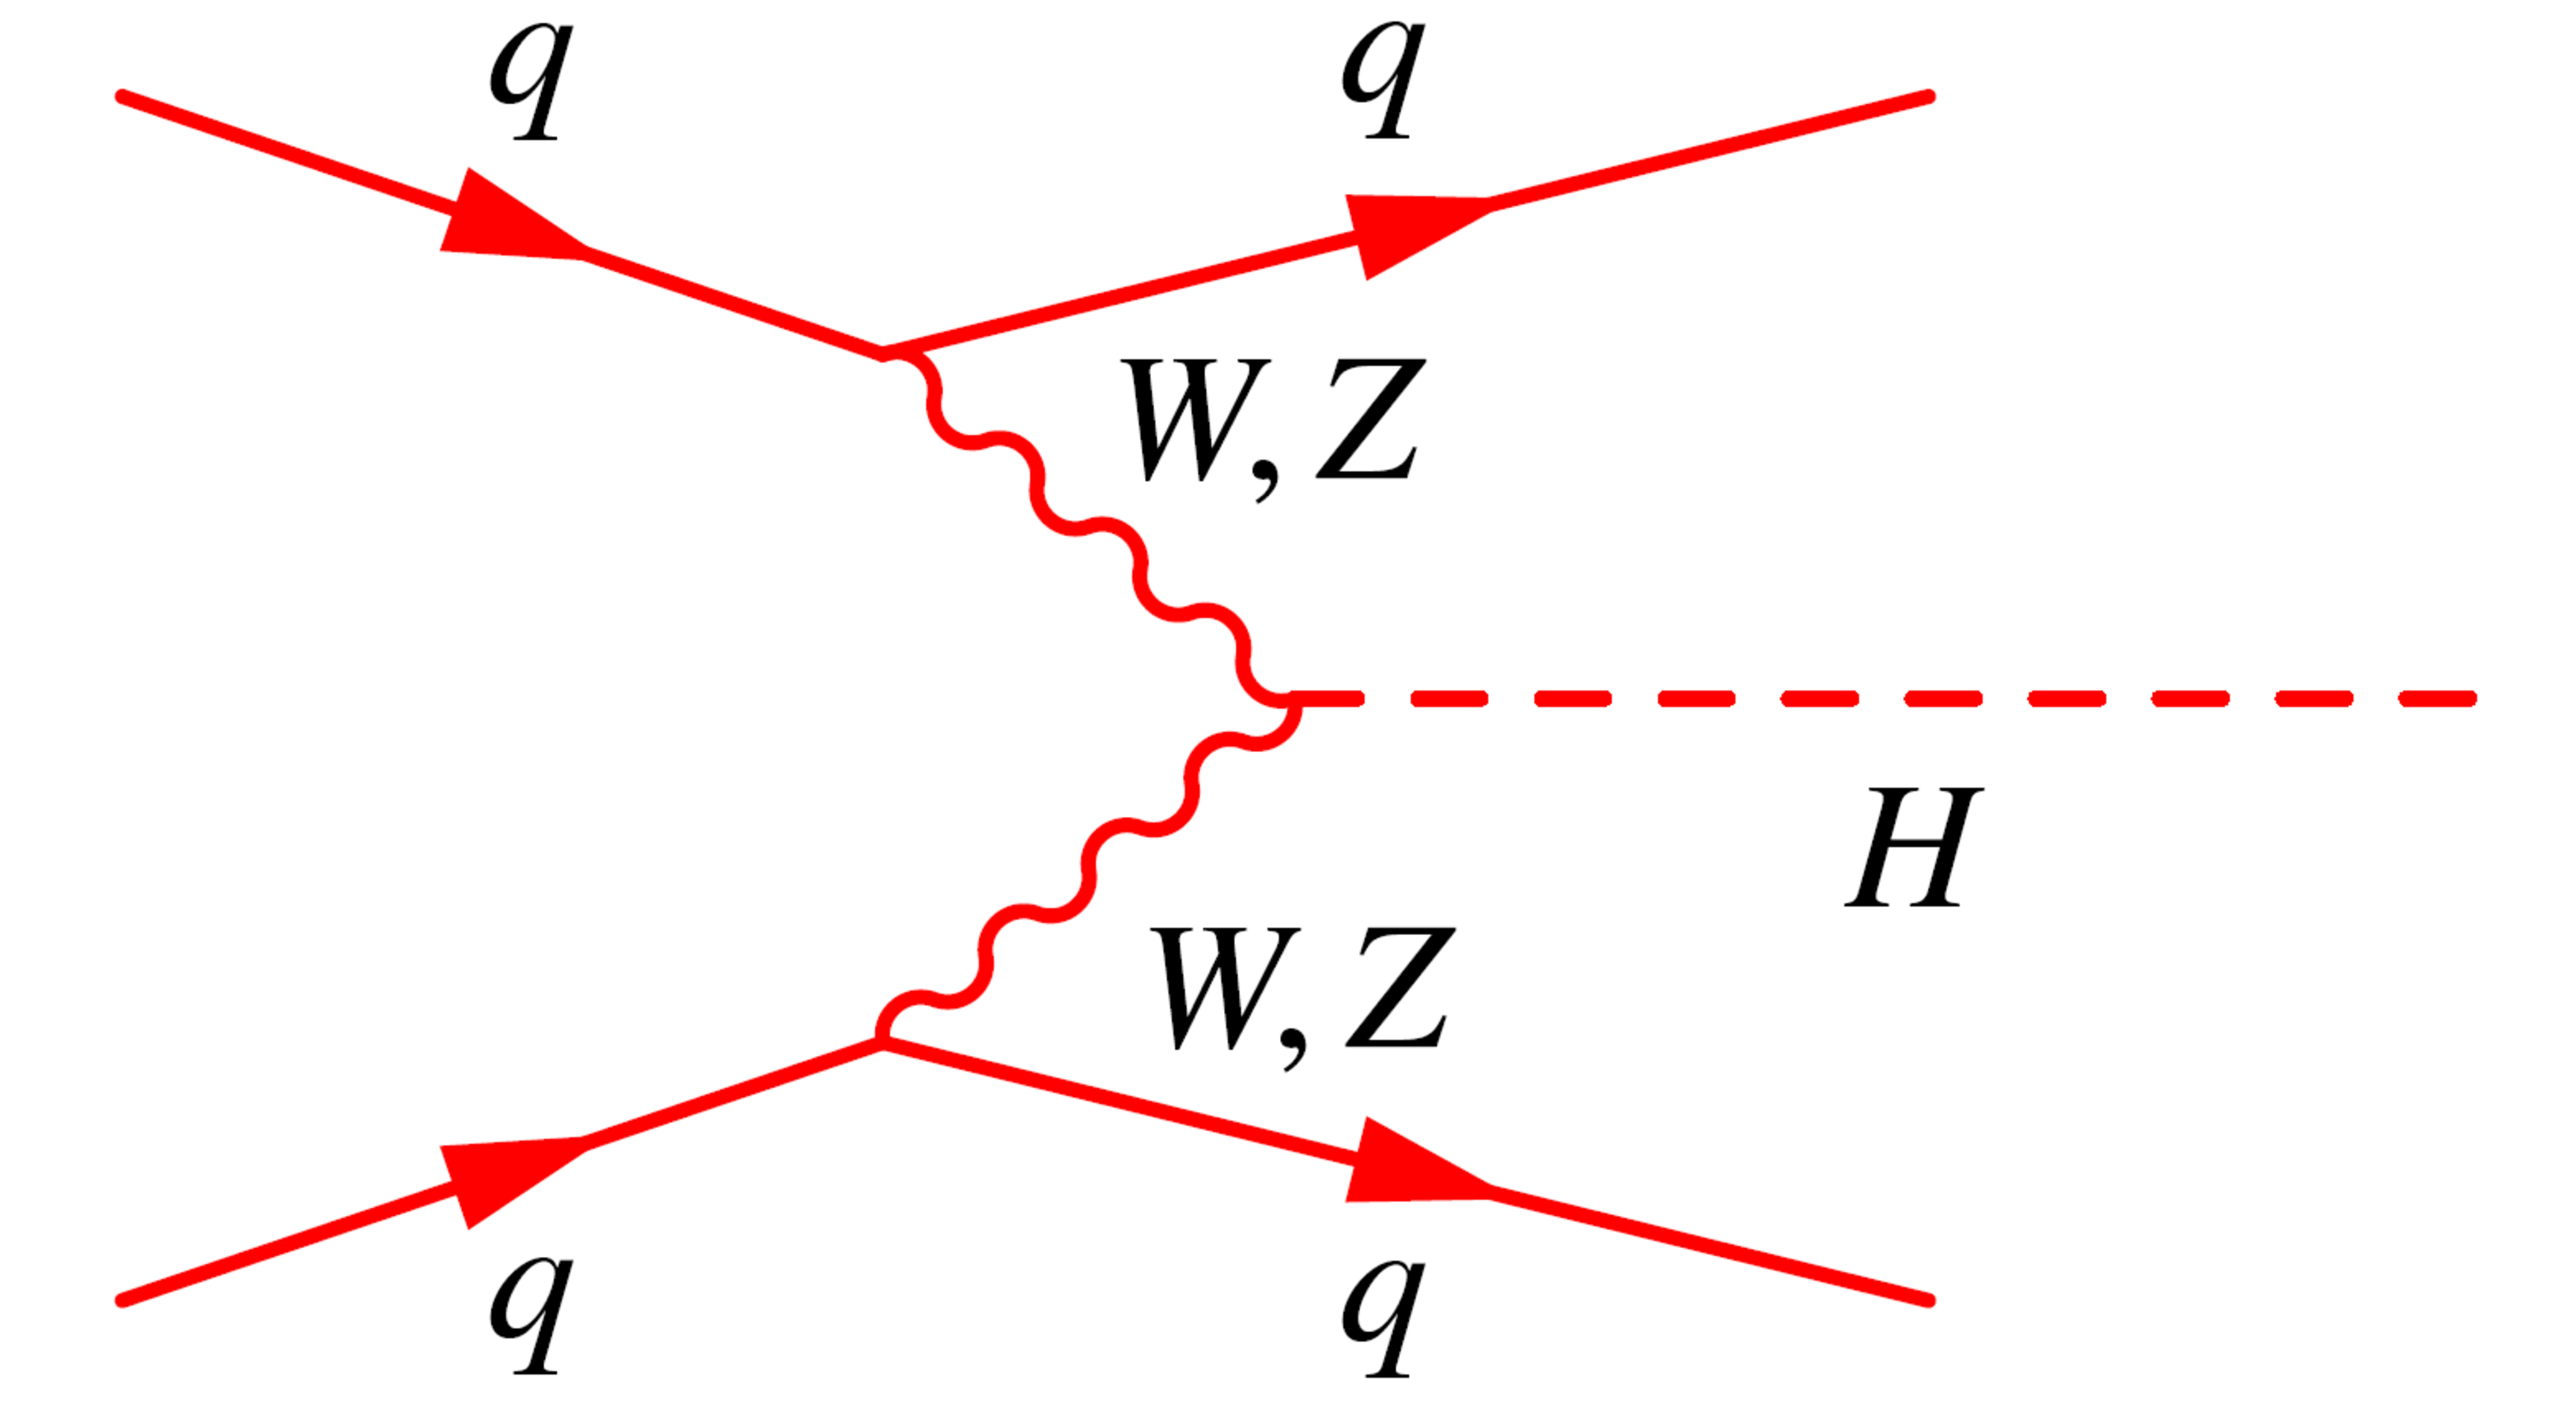
\includegraphics[width=0.45\textwidth]{images/VBF.pdf}
}\\
\subfigure[VH]{
 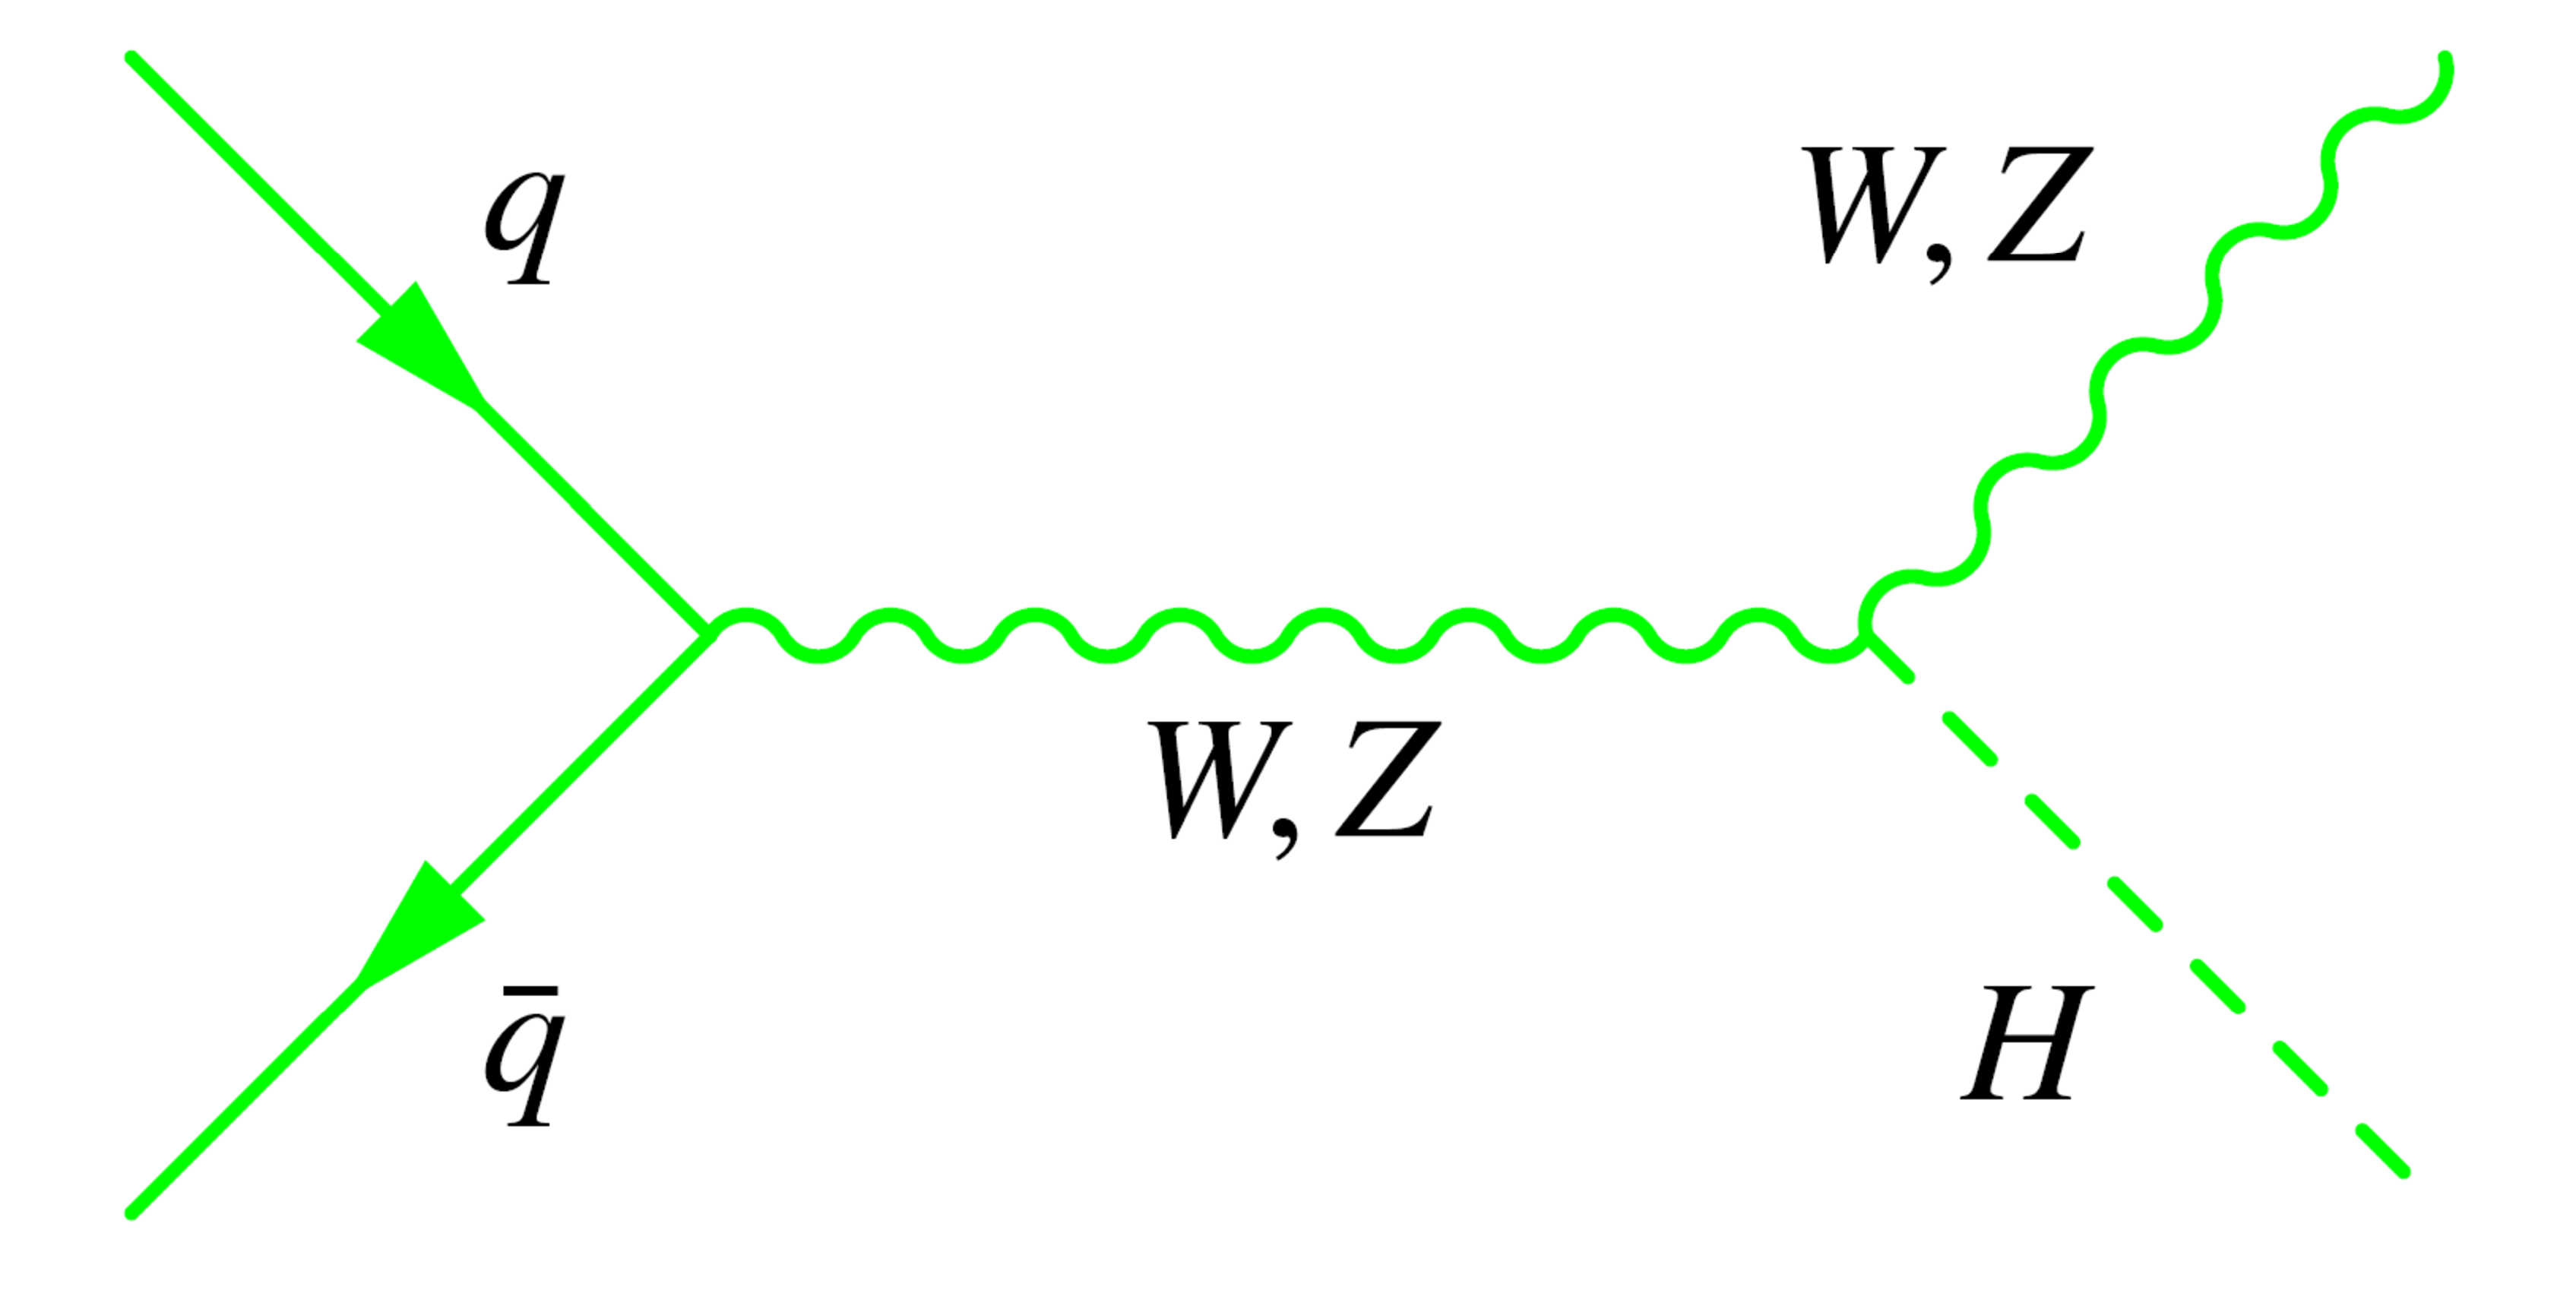
\includegraphics[width=0.45\textwidth]{images/VH.pdf}
}
\subfigure[\ttH]{
 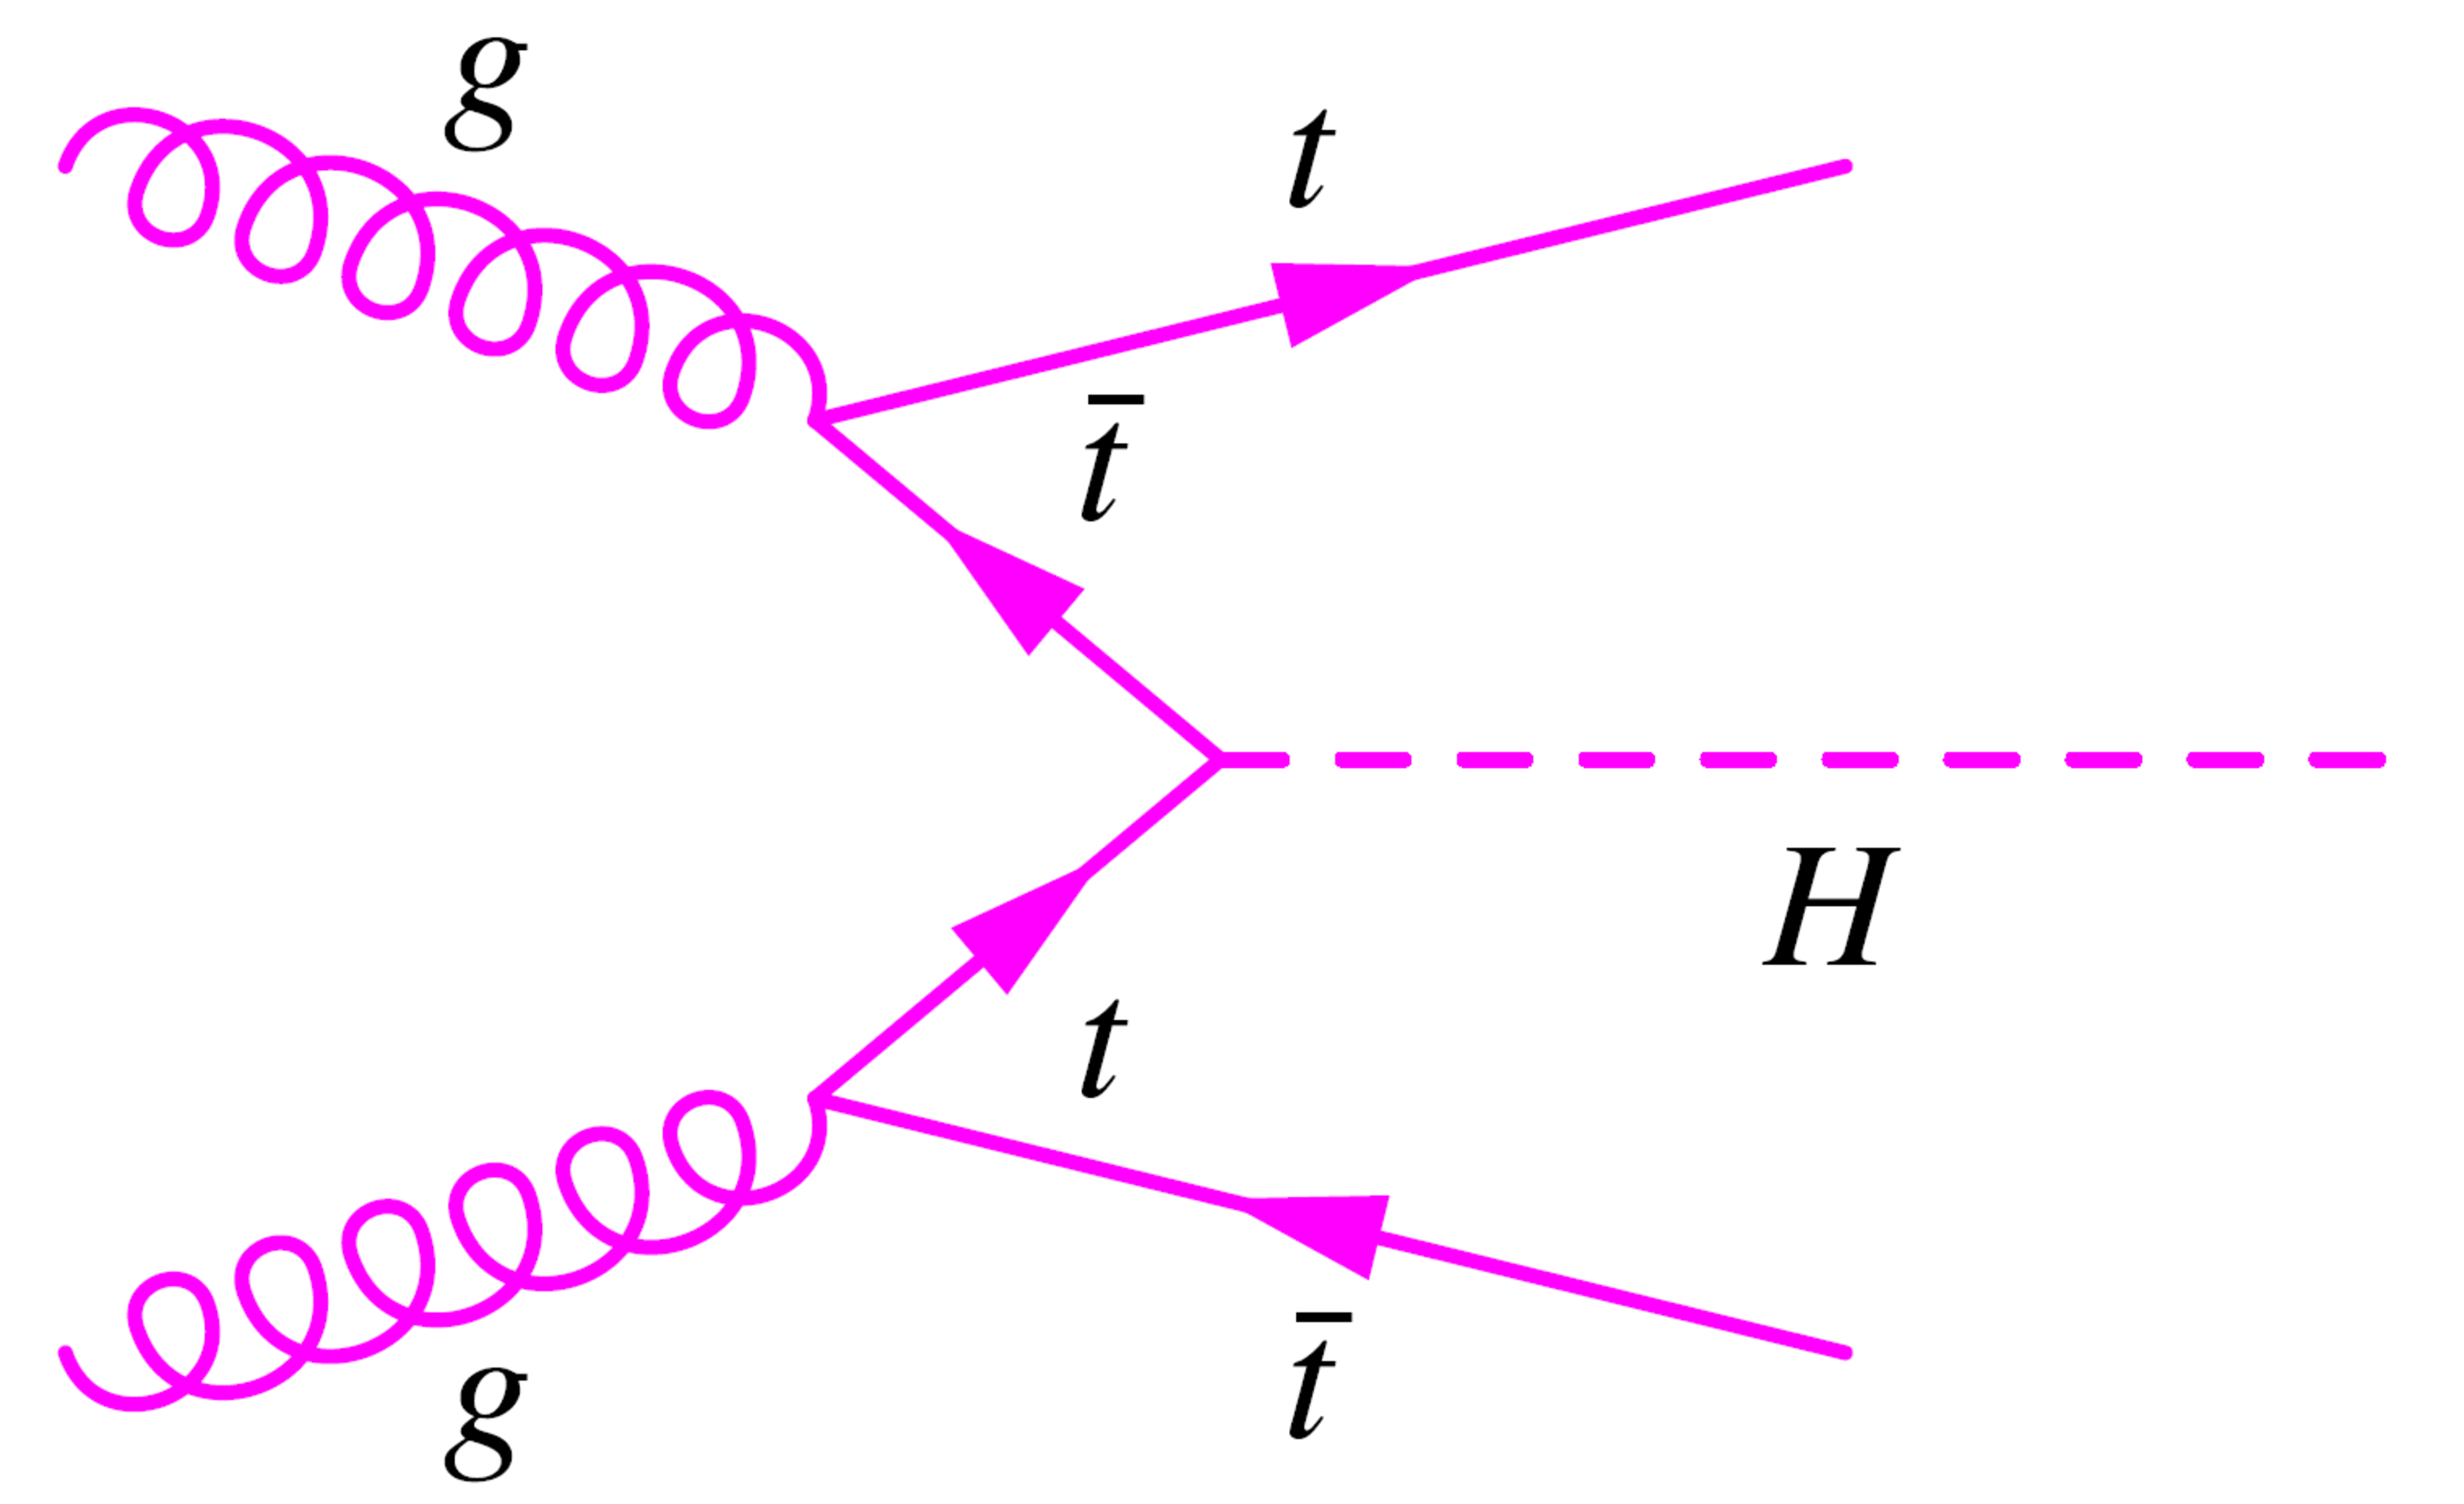
\includegraphics[width=0.45\textwidth]{images/ttH.pdf}
}
\caption{Main Higgs boson production processes at LHC.}\label{fig:higgs_prod}
\end{figure}

In order of decreasing cross section, the Higgs boson production modes are:

\begin{itemize}
\item \emph{Gluon fusion} (ggH): this is the main Higgs boson production mode at LHC over the whole mass spectrum. The process involves the fusion of two incoming gluons that give rise to the Higgs boson through a heavy quark loop, whose main contribution comes from the top quark, as shown in Fig.~\ref{fig:higgs_prod}(a).

\item \emph{Vector Boson Fusion} (VBF): each of the two interacting quarks emit a W or Z boson which, in turn, interact to produce the Higgs boson, as shown in Fig.~\ref{fig:higgs_prod}(b). Quarks deriving from the incoming partons after the emission of vector bosons proceed in the forward direction and represent the peculiar signature of this production mode, i.e. two high energy forward jets separated by a large pseudorapidity gap. This process has a cross section which is one order of magnitude lower than ggH for a large range of $m_\mathrm{H}$ values and it becomes comparable to ggH only for masses of the order of 1\TeV.

\item \emph{Vector boson associated production} (VH): also known as \emph{Higgsstrahlung}, this process is characterized by the emission of a Higgs boson from a $\mathrm{W}^\pm$ or Z boson produced by two incoming quarks, as depicted in Fig.~\ref{fig:higgs_prod}(c). The VH cross section is several orders of magnitude lower than the ggH and VBF cross sections.

\item \emph{Top quark associated production} (\ttH): a pair of top quarks, originated from the splitting of two incoming gluons, interacts to give rise to a Higgs boson, as illustrated in Fig.~\ref{fig:higgs_prod}(d).
\end{itemize}

\noindent Another production mechanism analogous to the \ttH process and with a similar cross section is the b quark associated production.

The SM Higgs boson production cross section for the various production modes depends on the Higgs boson mass and on the centre-of-mass energy, as shown in Fig.~\ref{fig:higgs_xsec}. In general, the production cross section of all processes decreases with increasing the Higgs boson mass, while the raise of the centre-of-mass energy reflects in an increase of the cross section over the whole mass range.

\begin{figure}[htb]
\centering
\subfigure{
 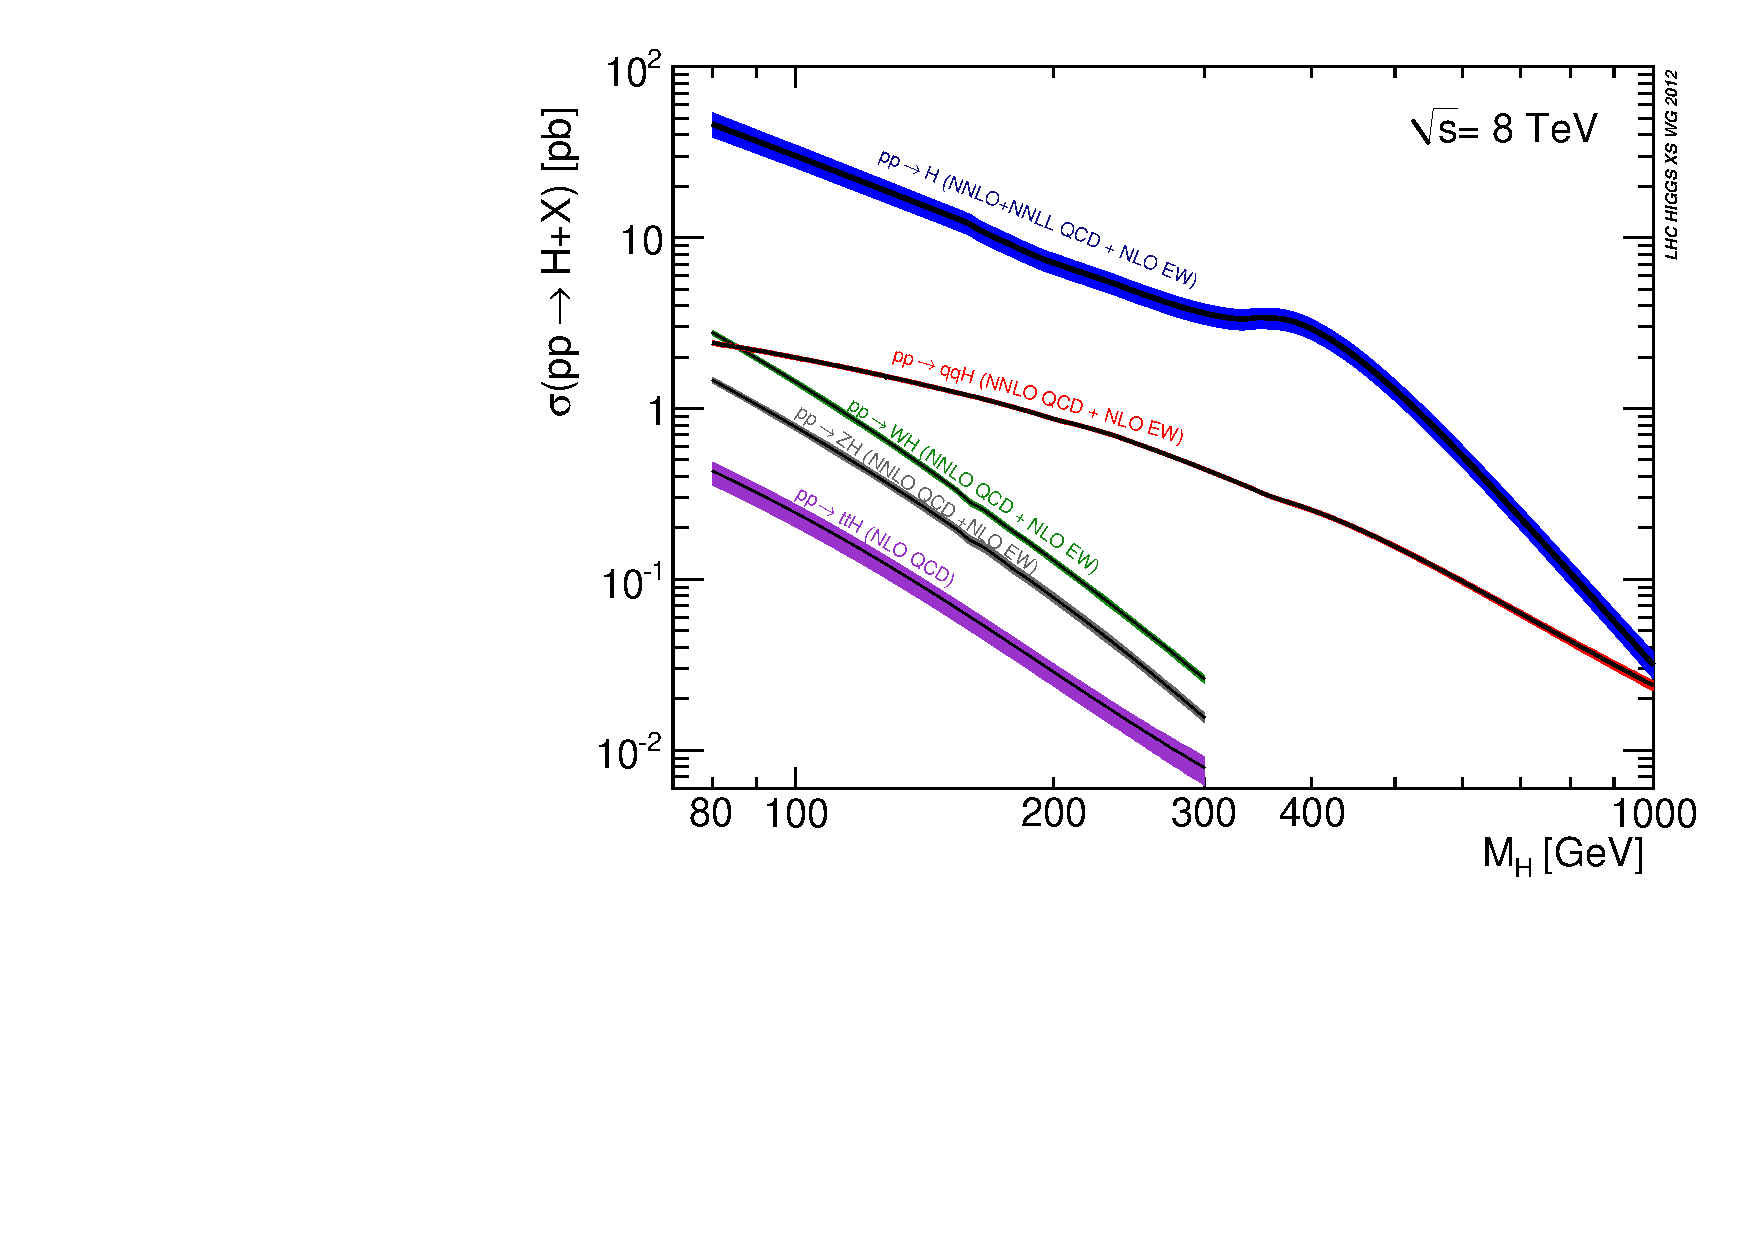
\includegraphics[width=0.45\textwidth]{images/XS_8TeV.pdf}
}
\subfigure{
 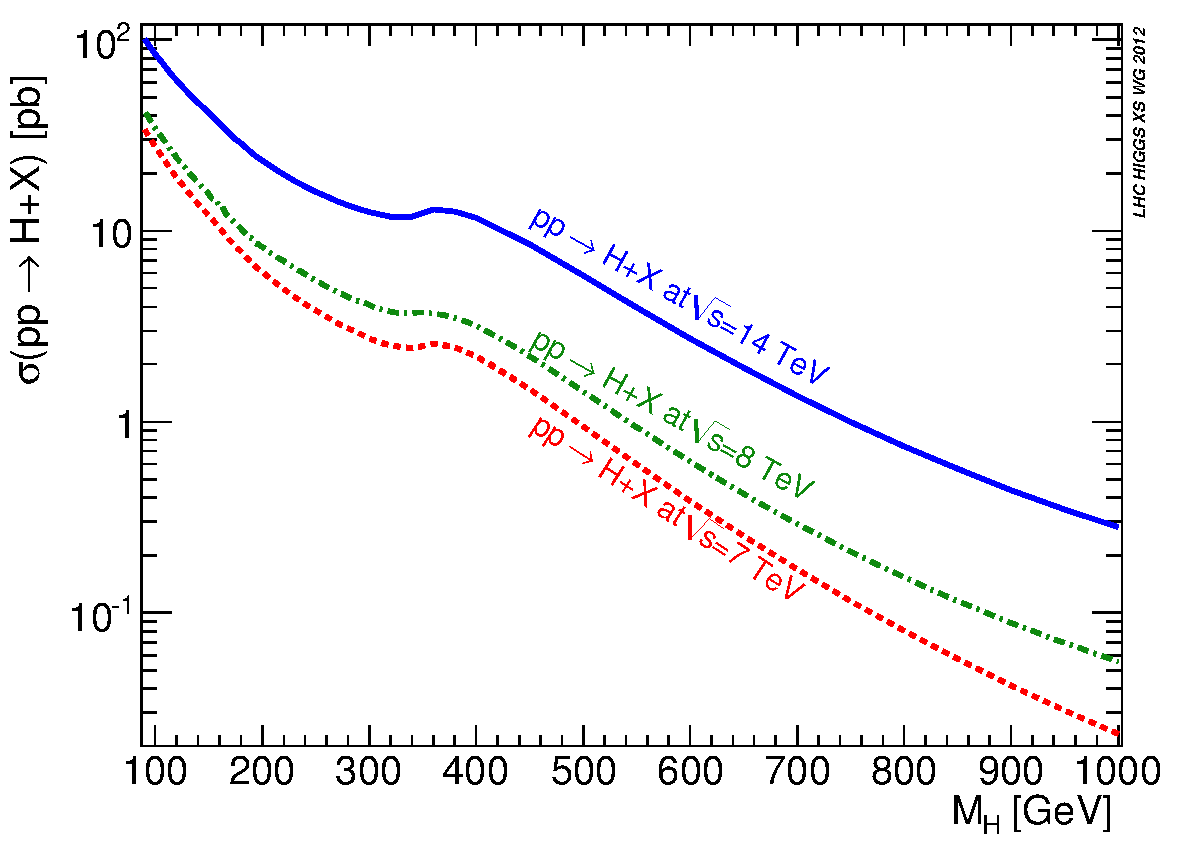
\includegraphics[width=0.45\textwidth]{images/totalXS.pdf}
}
\caption{Higgs boson cross section as a function of $m_\mathrm{H}$ for the various production mechanisms (left) and for different centre-of-mass energies (right).}\label{fig:higgs_xsec}
\end{figure}

The Higgs boson can decay to a variety of final states that can be divided in bosonic channels, like $\gamma\gamma$, ZZ or $\mathrm{W^+W^-}$, and fermionic channels, like $\tau\tau$, $\mathrm{b\bar b}$, etc.
Its branching ratio depends on the Higgs boson mass, as illustrated in Fig.~\ref{fig:higgs_br}, where different decay channels are compared over the whole mass spectrum. At $m_\mathrm{H} = 125$\GeV the decay channel with the largest branching ratio is $\mathrm{b\bar b}$, followed by WW, $\tau\tau$, ZZ and others. Although being the channel with the largest branching ratio, analyses looking at the H$\to \mathrm{b \bar b}$ decays are in practical cases limited by the overwhelming background contribution, which makes it possible only if the Higgs boson is produced via VBF, VH or \ttH, where additional jets or leptons can be used to tag the events.

The branching ratio to the WW and ZZ decay channels are instead dominant when increasing the Higgs boson mass, because the decays to real vector boson pairs become energetically allowed. In particular, the H$\to \mathrm{W^+W^-}$ decay channel, which is described in Sec.~\ref{sec:HWW}, is the second channel in terms of signal yield at $m_\mathrm{H} = 125$\GeV and the first one for higher mass values. Moreover, these channels are characterized by a much cleaner signature if the leptonic decays of one or both vector bosons are sought.

\begin{figure}[htb]
\centering
%\subfigure{
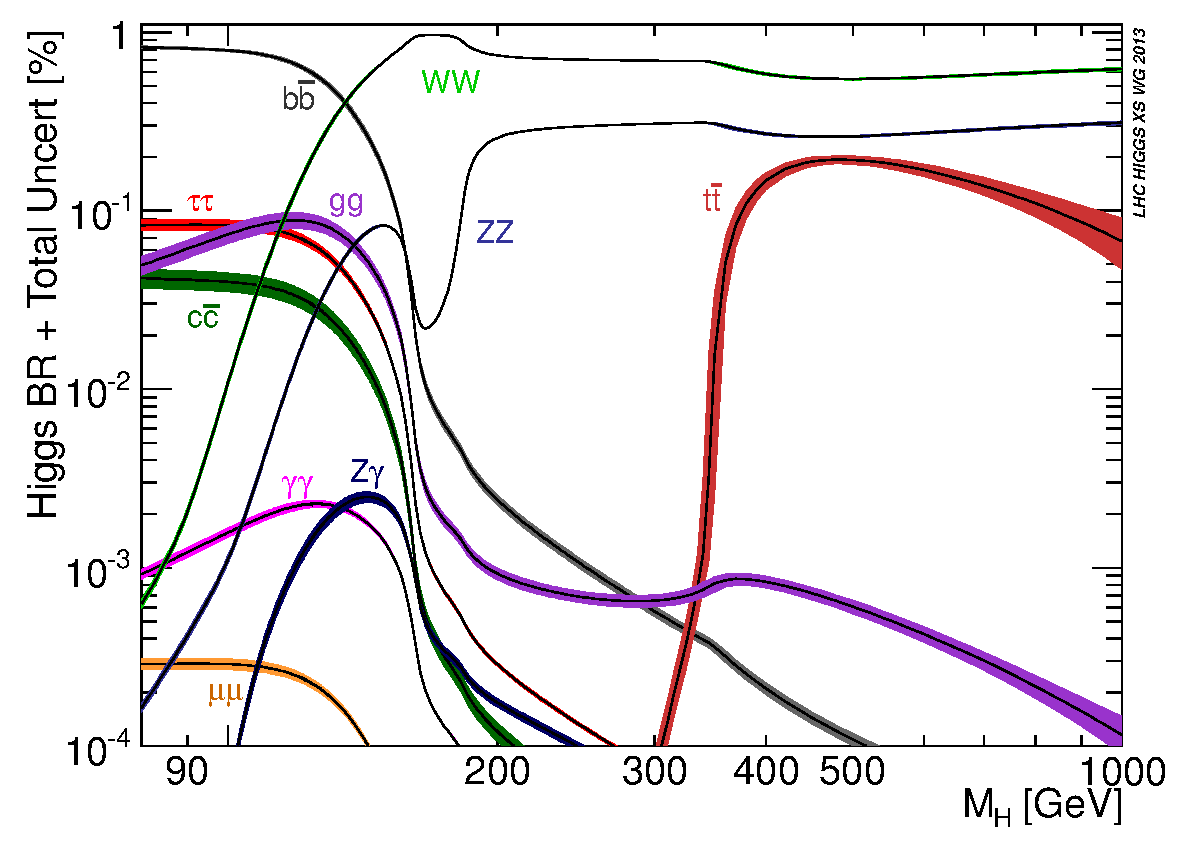
\includegraphics[width=0.6\textwidth]{images/Higgs_BR.pdf}
%}
%\subfigure{
% 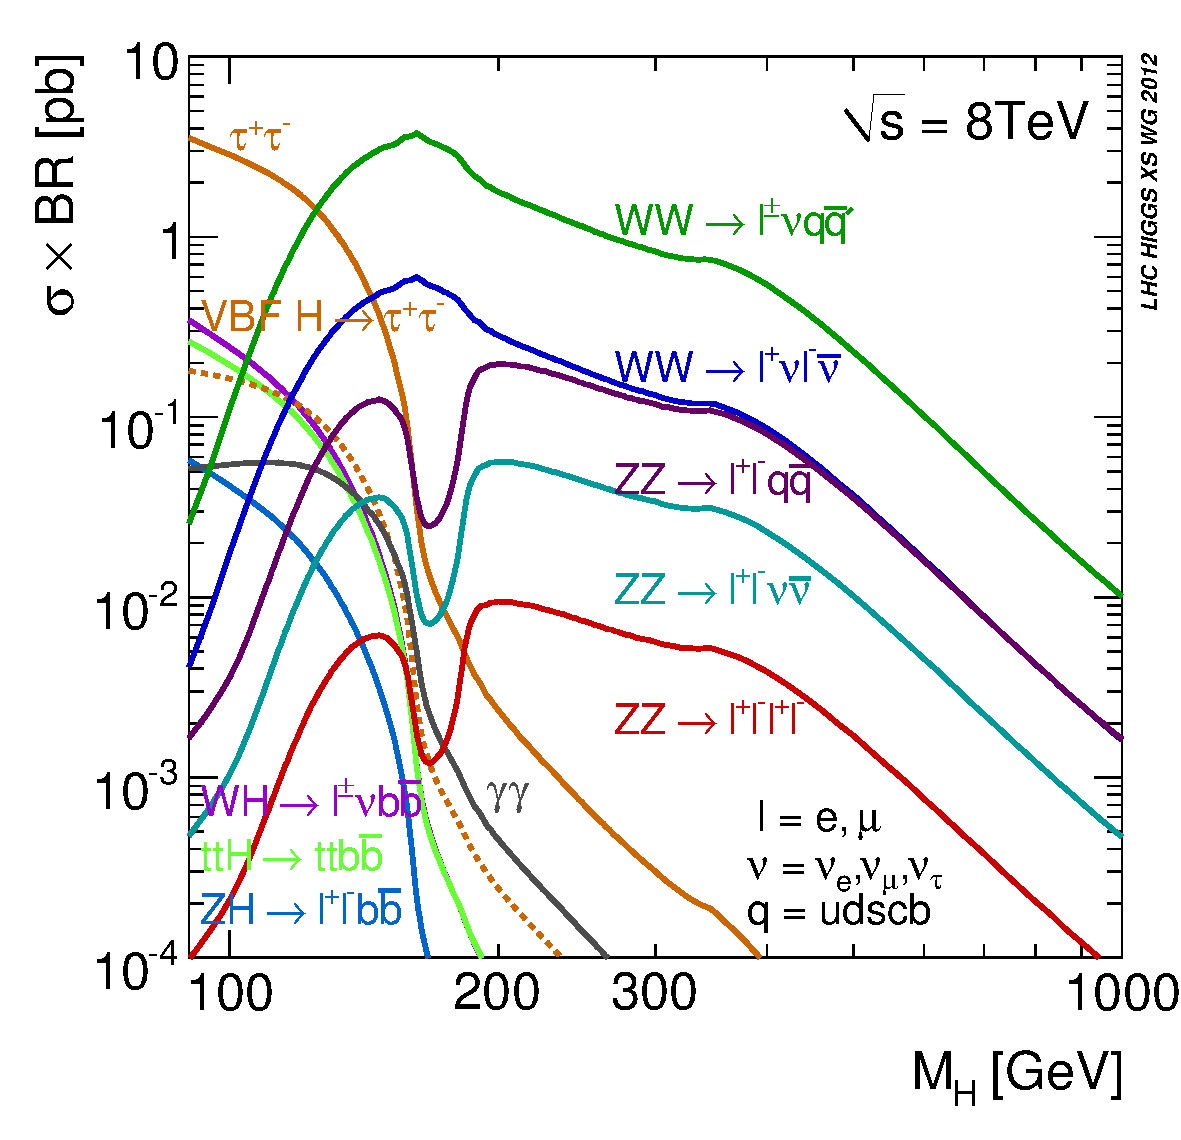
\includegraphics[width=0.45\textwidth]{images/Higgs_BR_2.pdf}
%}
\caption{Higgs boson branching ratio for all the decay channels as a function of $m_\mathrm{H}$.}\label{fig:higgs_br}
\end{figure}



%%%%%%%%%%%%%%%%%%%%%%%%%%%%%%%%%%%%%%%%%%%%%%%%%%%%%%%%%%%%%%%%%%%%%%
\subsection{The \hww decay channel}\label{sec:HWW}
As stated in the previous section, the \hww decay channel is one of the channels with the largest branching ratio across the full Higgs boson mass range. For Higgs boson masses below two times the W boson mass, $m_\mathrm{H} < 2m_\mathrm{W}$, the decay to two real W bosons is energetically forbidden, therefore one of the two is produced \emph{off-shell}. The W boson can in turn decay to hadrons, with a branching ratio of 67.41\%, or to leptons ($\mathrm{W}\to\ell\nu$) with a branching ratio of 10.86\%. The fully hadronic decay $\mathrm{H\to W^+W^- \to 4q}$ is thus the most probable decay mode, but the presence of four jets in the final state makes it hard to separate the signal from the overwhelming background contribution. The semi-leptonic final state, where one W boson decays to leptons and the other to hadrons, still has a large branching ratio and the presence of one electron or muon can be exploited to tag the events. Nevertheless the background contribution is, even in this case, very large.

The analyses presented in this work are focused on the fully leptonic final state (\hwwllnn) which, despite the lower branching ratio with respect to the other decay modes, is characterized by a clean signature and affected by much less background contribution. The signature of this final state is characterized by two leptons with opposite charge and a moderate amount of missing transverse energy, due to the presence of two neutrinos in the final state. In general the two leptons are characterized by high \pt values and, in case one of the W boson is off-shell (as for the SM Higgs boson case), the corresponding lepton has on average a smaller \pt with respect to the one arising from the on-shell W boson.

The final state with two same flavour leptons is not taken into account in the analyses discussed in this work, since it provides a smaller signal significance with respect to the different flavour case due to the presence of the huge contamination from Drell-Yan background processes.

Because of the presence of missing transverse energy in the final state, is not possible to reconstruct the full Higgs boson mass in this channel, and other methods must be used to distinguish between signal and background contributions.

The most important background processes contributing to this final state are non-resonant $\mathrm{q\bar q \to W^+W^-}$ and \ttbar production, whose Feynman diagrams are illustrated in Fig.~\ref{fig:wwandtop}. The first one is characterized by a final state identical to the signal, while the latter has two additional b quarks arising from the top quark decay. Despite the same final state, the lepton kinematics for signal and $\mathrm{q\bar q \to W^+W^-}$ processes is rather different. For the signal process, the W boson originates from a spin-0 particle decay and their spins must therefore be antiparallel, implying that the charged leptons produced in their decays appear preferentially in the same hemisphere~\cite{Ellis:2012wg}. In contrast, there is no preferential spin direction in the background case.
For this reason the azimuthal angle difference between the two leptons is on average smaller for signal than for background, resulting in a smaller dilepton invariant mass in the former case.

\begin{figure}[htb]
\centering
\subfigure[$\mathrm{q\bar q \to W^+W^-}$]{
  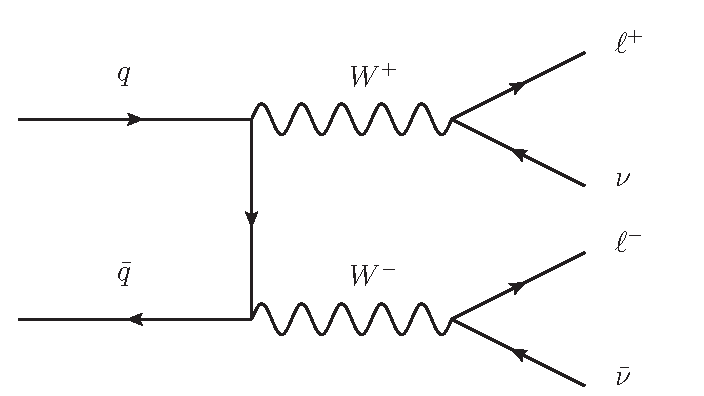
\includegraphics[width=0.4\textwidth]{images/WW.pdf}
}
\subfigure[\ttbar]{
  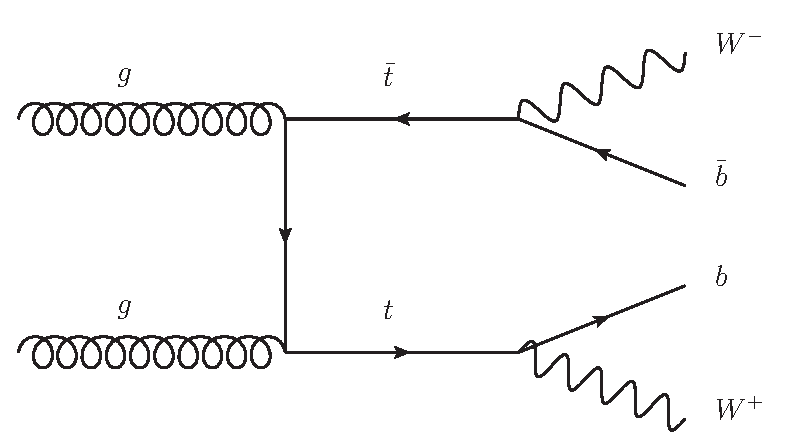
\includegraphics[width=0.4\textwidth]{images/ttbar.pdf}
}
\caption{Feynman diagrams corresponding to the $\mathrm{q\bar q \to W^+W^-}$ (left) and \ttbar (right) processes. The \ttbar diagram represents just one of the possible ways to produce a pair of top quarks at hadron colliders.}\label{fig:wwandtop}
\end{figure}

Other sub-dominant backgrounds arise from single top quark (tW, s-channel or t-channel), Drell-Yan, W+jets, di-boson and tri-boson processes.


%%%%%%%%%%%%%%%%%%%%%%%%%%%%%%%%%%%%%%%%%%%%%%%%%%%%%%%%%%%%%%%%%%%%%%
\subsection{Higgs boson kinematics}

The Higgs boson production at hadron colliders is kinematically characterized by its transverse momentum, \pth, and pseudorapidity, $\eta$. The $\eta$ distribution is essentially driven by the PDF of the partons in the colliding hadrons and it is only mildly sensitive to radiative corrections. The \pth distribution is instead sensitive to QCD radiative corrections. 
Considering the ggH production mode, at LO in perturbation theory, $\mathcal{O}(\alpha_s^2)$, the Higgs boson is always produced with \pth equal to zero. Indeed in order to have \pt different from zero, the Higgs boson has to recoil at least against one parton. Higher order corrections to the ggH process are numerically large and are known at NLO including full top quark mass dependence~\cite{Spira:1995rr,Harlander:2005rq}, and at NNLO using the so-called large-$m_\mathrm{t}$ approximation~\cite{Ravindran:2003um,Catani:2007vq,Anastasiou:2015ema}, in which the top quark mass is assumed to be very large and the fermionic loop is replaced by an effective vertex of interaction. Starting from the NLO, the Higgs boson can be produced recoiling against other final state partons, resulting in finite \pth values. For this reason the LO process for Higgs production at $\pt \neq 0$ is at $\mathcal{O}(\alpha_s^3)$, and the counting of perturbative orders differs between inclusive Higgs boson production and \pth distribution. Also, NNLO QCD corrections in the \pth observable have recently been shown~\cite{Chen:2016zka}.

When $\pth \sim m_\mathrm{H}$ the QCD radiative corrections to \pth differential cross section are theoretically evaluated using fixed-order calculations. When $\pth \ll m_\mathrm{H}$ the perturbative expansion does not converge due to the presence of large logarithmic terms of the form $\alpha_s^n \ln^{2n}m_\mathrm{H}^2/\pt^2$, leading to a divergence of $d\sigma/d\pt$ in the limit of $\pt\to0$. For computing the \pth spectrum in this region, soft-gluon resummation techniques are used~\cite{Bozzi:2005wk,deFlorian:2012mx}, and matched to the fixed-order calculation in the $\pth \sim m_\mathrm{H}$ region.
For the \pth differential cross section the large-$m_\mathrm{t}$ calculation is a crude approximation, since it is known that the top quark mass has a non-negligible effect on the shape of the spectrum. Moreover the inclusion of the bottom quark contribution in the fermionic loop can significantly modify the \pth shape~\cite{Grazzini:2013mca}, as shown in Fig.~\ref{fig:pth_quarkmass}. Hence, a precise experimental measurement of the \pth spectrum is important to test the existing SM calculations. 

\begin{figure}[htb]
\centering
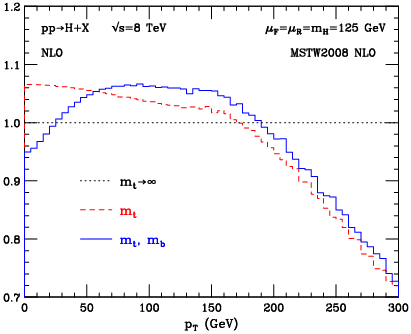
\includegraphics[width=0.5\textwidth]{images/pth_quarkmass.png}
\caption{Distribution of \pth computed at NLO ($\alpha_s^4$) and divided by the calculation obtained in the large-$m_\mathrm{t}$ approximation. The red dashed line corresponds to the calculation including the top quark mass while the blue line refers to the calculation including also the bottom quark effects.}\label{fig:pth_quarkmass}
\end{figure}

Possible extensions of the SM predict a modification of the Higgs boson couplings to gluons and top quarks. Many of these models actually predict the existence of new states that interact with the SM Higgs boson but are beyond the direct production reach at the actual LHC energies. The effect of these new states could however show up as a deviation of the Higgs boson couplings with respect to the SM expectation. The modification of the couplings, as shown in Refs.~\cite{Azatov:2013xha,Harlander:2013oja}, can change the kinematics of the Higgs boson production and the effect can be particularly sizeable in the tail of the \pth distribution. 
Other models, such as Composite Higgs~\cite{Marzocca:2012zn}, predict the existence of top-partners, which are heavy resonances with the same quantum numbers as the top quark, that can interact with the Higgs boson in the ggH fermionic loop, changing the \pth shape with respect to what the SM predicts~\cite{Banfi:2013yoa}.
The measurement of the \pth spectrum is thus a useful tool for indirect searches of new particles predicted by theories beyond the SM.





%%%%%%%%%%%%%%%%%%%%%%%%%%%%%%%%%%%%%%%%%%%%%%%%%%%%%%%%%%%%%%%%%%%%%%
\subsection{Event generators for Higgs boson production}

The structure of events produced at high energy colliders is extremely complex, and complex numeric simulations are necessary to effectively simulate realistic events. Monte Carlo (MC) event generators are programs that subdivide the problem of producing realistic events into a sequence of tasks that can be handled separately with the help of both analytic and numeric computations.

The production of hadron-hadron collision events is the result of the following chain of calculations:

\begin{itemize}
\item the first step consists in the calculation of cross section for the selected process, considering partons extracted from the incoming hadrons as free particles;

\item the event production starts with two colliding hadrons with given momenta. One parton out of each hadron is selected to enter the scattering process of interest. This step is often referred to as \emph{hard scattering} generation. Final state partons and leptons are produced according to the calculated differential cross sections;

\item resonances produced in the hard event are decayed;

\item when two partons take part in the hard event, accelerated colour charges are present, thus bremsstrahlung can occur. This effect is called initial state radiation (ISR) and is simulated with the so called \emph{Initial State Parton Showers} algorithm, using the knowledge of the PDFs;

\item also the final state partons can produce further radiation, called final state radiation (FSR), which is simulated by the \emph{Final State Parton Showers} algorithms;

\item in addition to the partons taking part in the hard interaction, several other parton pairs can interact during a hadron-hadron collision, giving rise to interactions with smaller transferred momentum. These \emph{multiple parton interactions} (MPI) contribute to the so called \emph{underlying event} (UE). Such interactions need to be well simulated to produce realistic events;

\item leftovers of the interacting hadrons need to be simulated to balance the colour charge
and four-momentum conservation. The beam remnant handling is thus another step in the event generation;

\item the partons produced in the final state after the hard scattering are not observed as free particles but are subjected to the hadronization process, that cannot be described with perturbative QCD and is simulated using empirical models;

\item finally, the event generator takes care of decaying $\tau$ leptons and B hadrons. Particles with very short lifetime are generally decayed by the generator itself, while those with longer lifetimes are left undecayed.
\end{itemize}

The calculation of the hard process cross section is performed using the Matrix Element (ME) method, which is available for a variety of processes and consists on the exact matrix element calculation of the Feynman diagram of the process of interest. This approach is performed using perturbative QCD calculations and provide an analytically exact solution. Tree-level cross sections can be calculated including up to several partons in the final state. Loop calculations are instead more complex and are available only for a limited set of processes. 

The ME method presents two complications: the first one arises from the presence in the calculation of partons with low transverse momentum (\emph{soft} divergence) and the second to situations in which the emitted parton is collinear to the radiating parton (\emph{collinear} divergence). Both these cases lead to divergences that spoil the perturbative calculation. The virtual corrections would cancel these divergences but, since at tree-level they are not included, the phase space has to be carefully tailored to avoid the problematic regions. This means that the matrix
element cross section calculations are performed away from soft and collinear divergences. Therefore, in order to produce realistic events, the phase space regions omitted in the ME calculation need to handled using a different method, the Parton Shower calculation.

Parton Shower (PS) algorithms offer an alternative way both to handle the complexity of several successive branchings and to remove soft and collinear divergences. The parton showers are described by the algorithm as a sequence of elementary events $a\to bc$, where each event can happen with a certain probability driven by the structure of perturbative QCD. The introduction of a threshold value
and the application of an angular sorting procedure in the emission of partons allows to eliminate soft and collinear divergences typical of the ME method. The parton cascade is evolved down to a certain virtuality, of the order of 1\GeV. After that, non perturbative effects take place and the hadronization is applied. Since the parton shower machinery relies on a collinear approximation of the matrix element, it is supposed to perform well in the description of the evolution of jets, but not to provide a precise description of configurations with well separated partons.

The two aforementioned techniques are therefore complementary and their combined application in the intermediate cases allows to exploit the characteristics of the two algorithms in the respective limits of validity. Several prescriptions exist to combine together the ME and PS calculations avoiding double-counting or holes in the phase space~\cite{Hoche:2006ph}.

In this work the \textsc{Powheg}~\cite{Kramer:2005hw,Frixione:2007vw,Lavesson:2008ah,Alioli:2008tz, Nason:2009ai} and \textsc{MadGraph} (and its evolution \textsc{MadGraph5\_aMC@NLO}) generators~\cite{Alwall:2014hca} are mostly used for the ME calculation, interfaced to \textsc{Pythia}~\cite{Sjostrand:2006za,Sjostrand:2007gs} for the PS and hadronization. 

\textsc{Powheg} is a ME event generator that performs calculations with NLO QCD accuracy and provides an easy prescription for the interface to PS programs. It can be used to generate events corresponding to a large number of predefined processes. It is used for the simulation of the majority of the processes involving Higgs boson production, as ggH and VBF. The \textsc{JHUGen}~\cite{JHUGen} generator, which is capable to take into account all spin correlations, is usually employed together with \textsc{Powheg} to simulate the Higgs boson decay to whatever final state is desired. In the analyses described in Chapter~\ref{chap4} two versions of this generator are used for simulating events produced via the ggH mechanism: \textsc{Powheg V1} and the more recent \textsc{Powheg V2}, which takes into account the finite mass of the bottom and top quarks in the ggH loop.

\textsc{MadGraph5\_aMC@NLO} is a software that allows to generate amplitudes and events for any user defined process (with up to 9 external particles) with LO or NLO QCD accuracy.

\textsc{Pythia} is a general purpose generator. It contains a large subprocess library covering SM and BSM physics. It can be used standalone as a ME generator to perform cross section calculation and generate events at LO QCD accuracy, or interfaced to a ME generator like \textsc{Powheg} or \textsc{MadGraph5\_aMC@NLO} as a PS and for the simulation of the hadronization process.


\section{Experimental Higgs boson highlights}
%%%%%%%%%%%%%%%%%%%%%%%%%%%%%%%%%%%%%%%%%%%%%%%%%%%%%%%%%%%%%%%%%%%%%%
\label{sec:HiggsExp}

The discovery of the new boson has been followed by a comprehensive set of measurements aimed at establishing the properties of the particle. Latest results reported by both the ATLAS and CMS experiments are consistent with the SM expectations for the Higgs boson. The properties that have been measured are, mainly:

\begin{itemize}
\item the signal strength modifier $\mu = \sigma/\sigma_\mathrm{SM}$, where $\sigma$ is the observed production cross section and $\sigma_\mathrm{SM}$ is the value predicted by the SM for a given mass hypothesis;

\item the couplings to bosons and fermions;

\item the spin and parity;

\item the total decay width of the resonance.
\end{itemize}

Moreover, the combination of the results of the two experiments has recently been performed concerning the mass of the new boson, which is found to be $m_\mathrm{H} = 125.09 \pm 0.21 ~\text{(stat.)} \pm 0.11~\text{(syst.)}$\GeV~\cite{Aad:2015zhl}.

The CMS experiment has investigated the Higgs boson decays to ZZ, WW, $\gamma\gamma$, $\tau\tau$ and $\mathrm{b \bar b}$ using 2011 and 2012 data, and is now looking at the same channels using new data collected at a centre-of-mass energy of 13\TeV. The 8\TeV CMS results of all the channels have been combined and the best-fit signal strength corresponding to the measured mass is found to be $\mu = 1.00 \pm 0.09~\text{(stat.)} ^{+0.08}_{-0.07}~\text{(theo.)} \pm  0.07~\text{(syst.)}$~\cite{Khachatryan:2014jba}, in good agreement with the SM expectation $\mu=1$.
The signal strengths modifiers obtained in different sub-combinations of channels for $m_\mathrm{H}=125$\GeV are shown in Fig.~\ref{fig:signal_strengths}, grouped by production mode tag and decay channel.

\begin{figure}[htb]
\centering
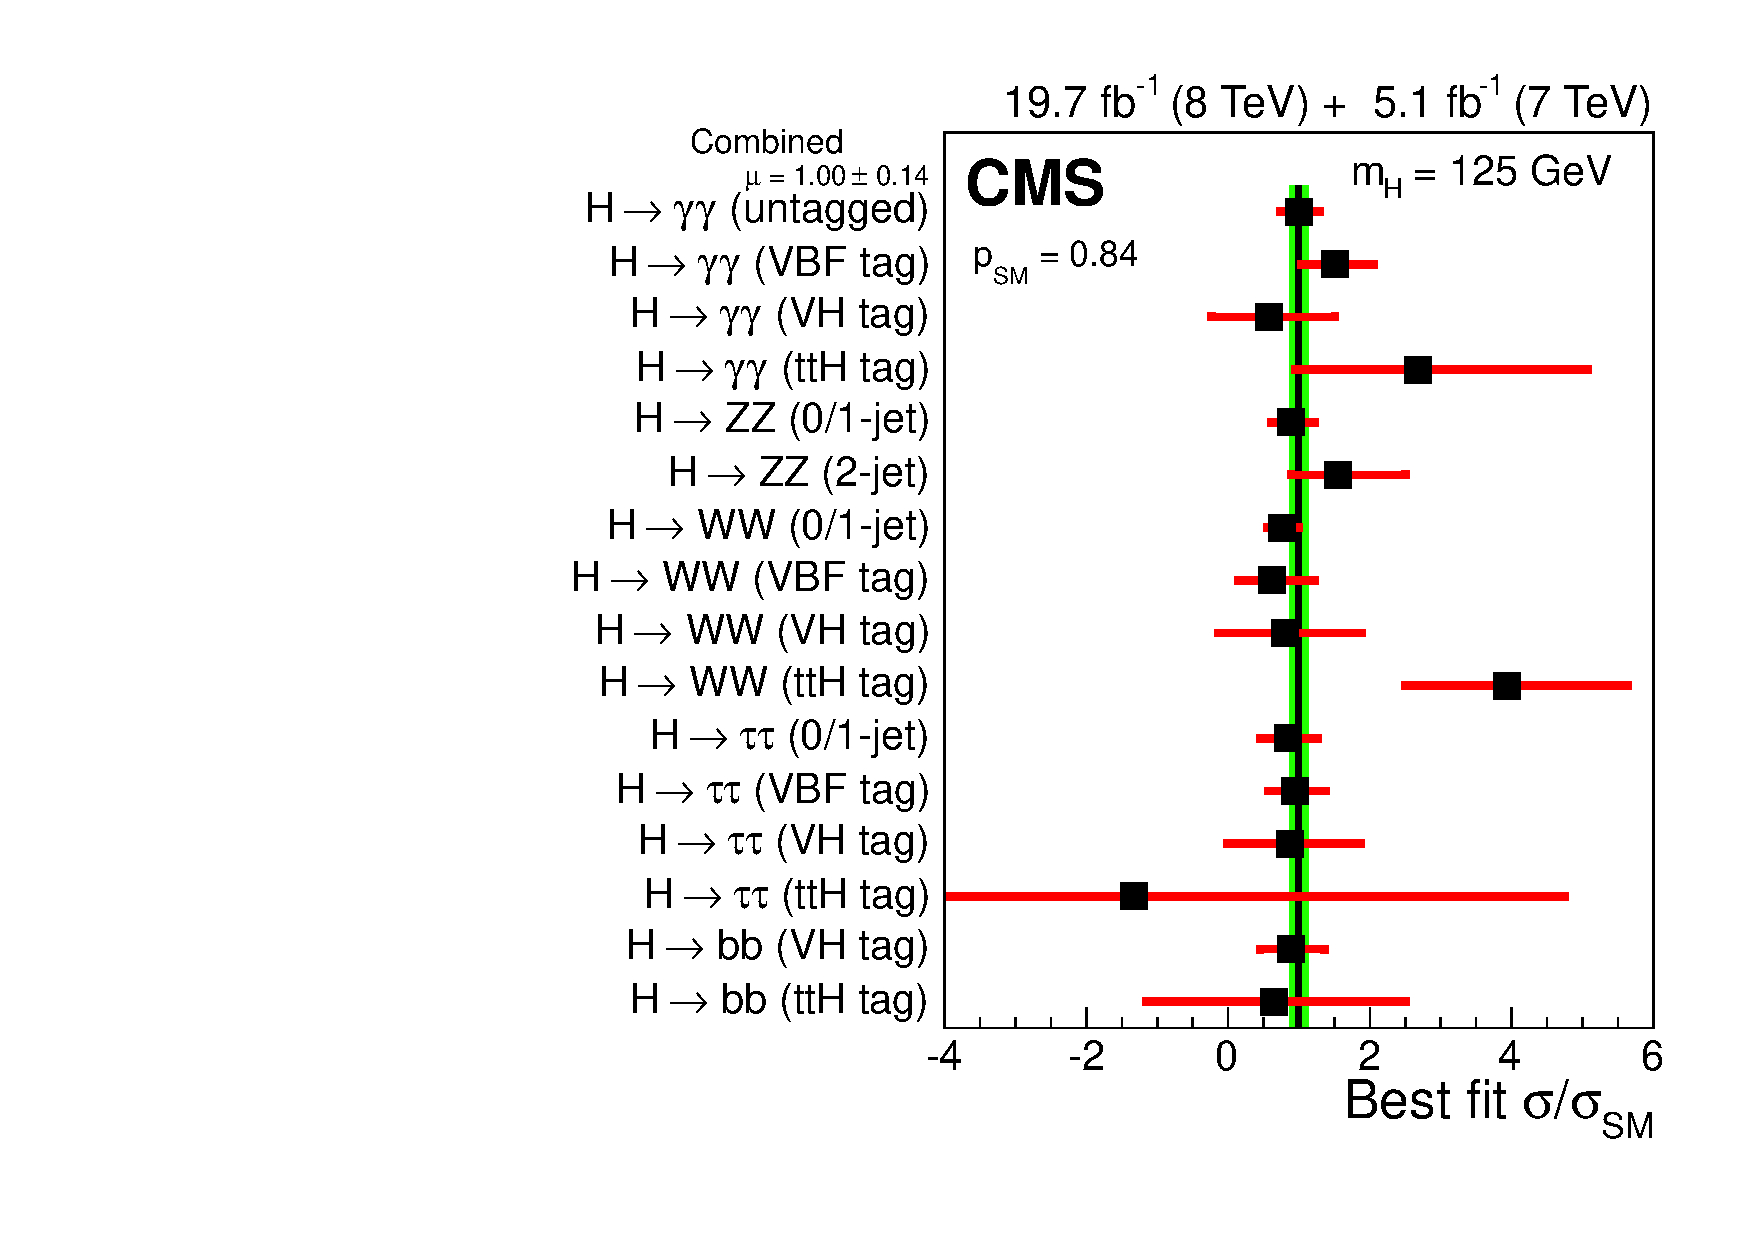
\includegraphics[width=0.7\textwidth]{images/signal_strengths.pdf}
\caption{Values of the best-fit $\mu$ for the overall combined analysis (solid vertical line) and separate combinations grouped by production mode tag and decay channel.}\label{fig:signal_strengths}
\end{figure}
    
The combination of all measurements in all decay channels is used to extract ratios between the observed coupling strengths and those predicted by the SM. The formalism used to test for deviations from the SM expectations has been established by the LHC Higgs Cross Section Working Group in Ref.~\cite{Heinemeyer:2013tqa}. This formalism makes some assumptions, in particular that the observed state has $J^P =0^+$ and that the narrow width approximation holds, leading to a factorization of the coupling strengths for production and decay modes. As an example, Higgs boson events produced via ggH and decaying to WW, i.e. $\mathrm{gg\to H\to WW}$, can be used to measure the Higgs boson coupling to W bosons and to fermions (mainly top quarks due to their presence in the gluon fusion loop). The combination of ATLAS and CMS results using data collected at 7 and 8\TeV is used to test the Higgs boson coupling to fermions $k_F$ and bosons $k_V$~\cite{Khachatryan:2016vau}. The contours at 68\% CL in the $(k_F^f, k_V^f)$ plane (where the $f$ refers to the generic decay channel H$\to f$) for the combination of ATLAS and CMS results and for the individual channels are shown in Fig.~\ref{fig:couplings}.

\begin{figure}[htb]
\centering
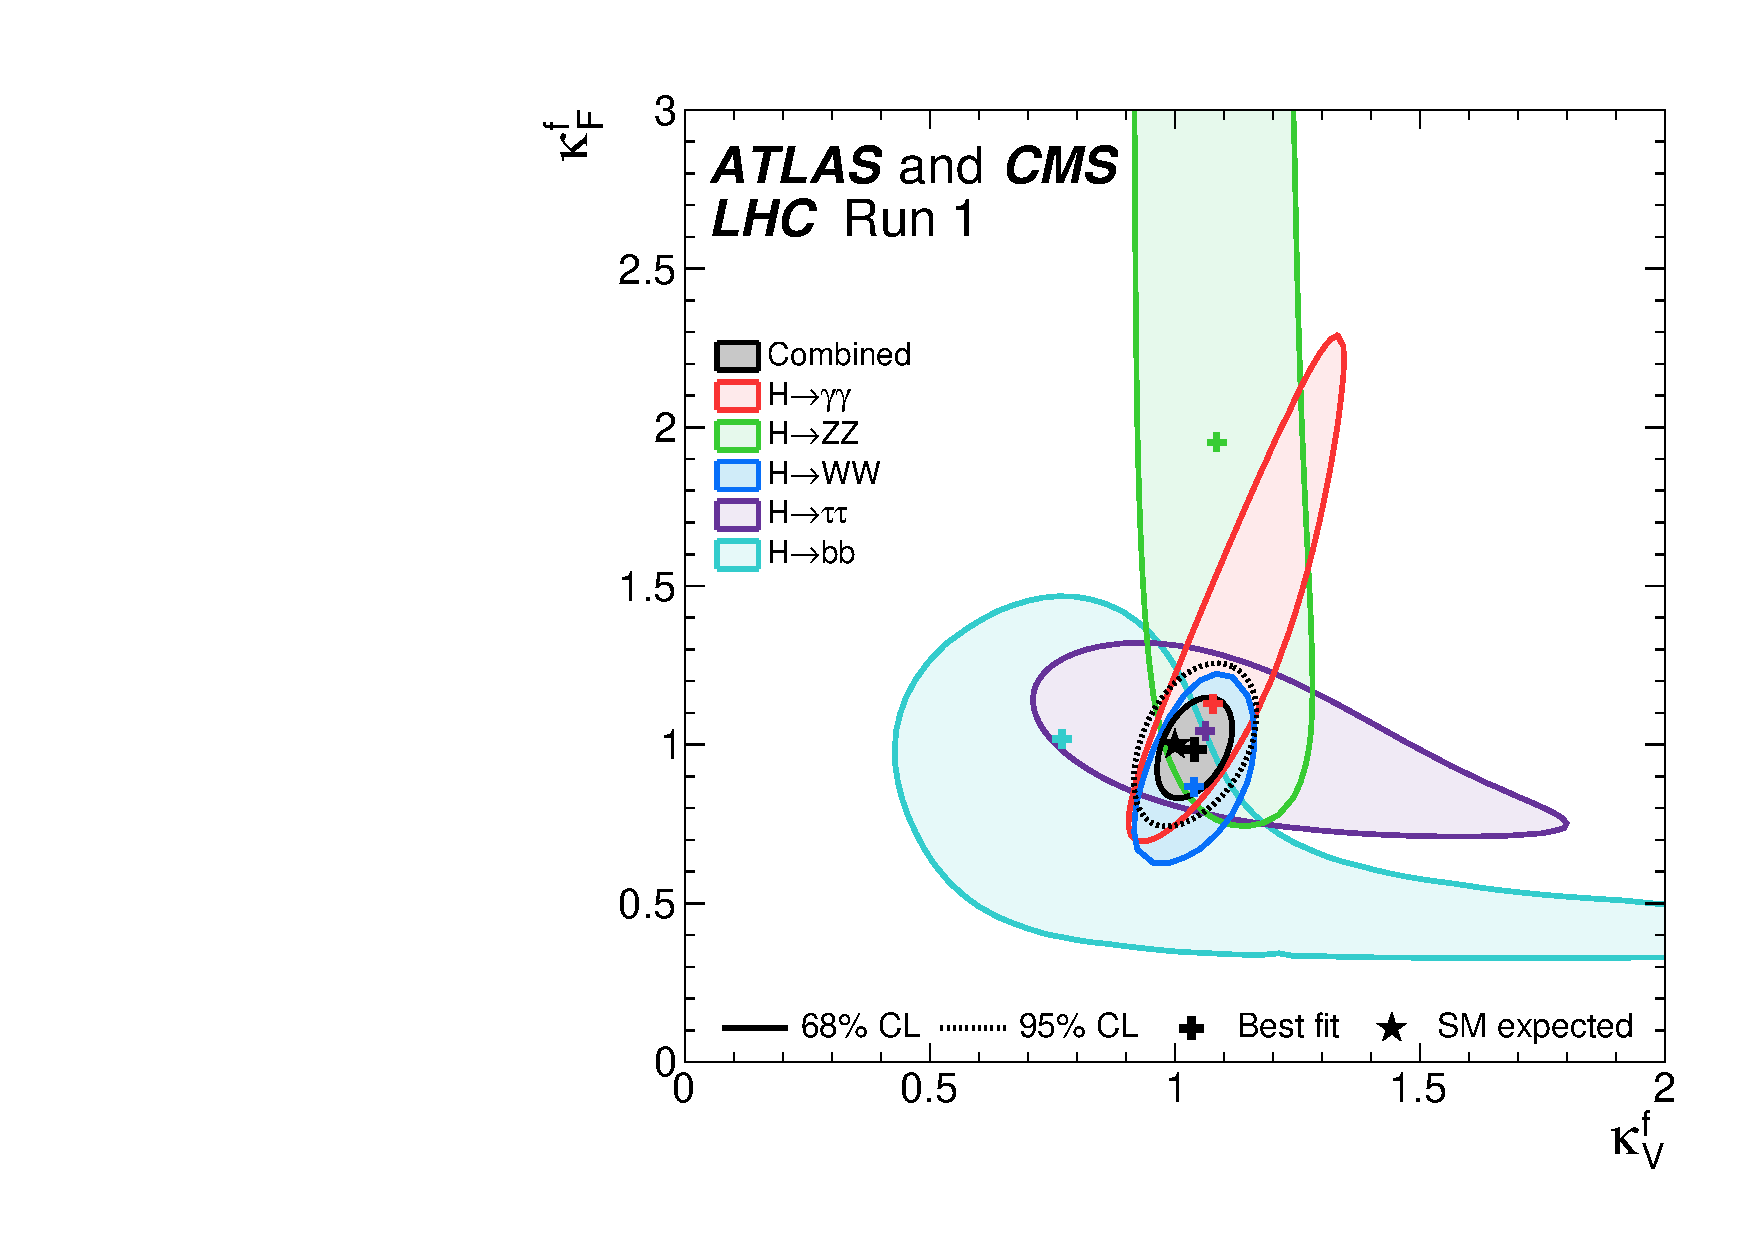
\includegraphics[width=0.7\textwidth]{images/couplings.pdf}
\caption{Contours at 68\% CL in the $(k_F^f, k_V^f)$ plane for the combination of ATLAS and CMS results and for the individual channels.}\label{fig:couplings}
\end{figure}

The combined result is in agreement with the SM expectation and the final confidence interval is driven by the \hww channel, which provides the most precise determination of $k_F^f$ and $k_V^f$ because it is the only channel that provides significant constraints on both parameters through the measurements of the ggH and VBF production processes.

About the spin and parity properties, the results of the H$\to \gamma\gamma$, H$\to$ZZ$\to 4\ell$ and \hwwllnn channels confirmed the hypothesis of a scalar boson ($J^P = 0^+$), excluding the other hypotheses with a confidence level of 99\% or higher.

The Higgs boson total decay width ($\Gamma_\mathrm{H}$) is predicted by the SM as a function of its mass, as shown in Fig.~\ref{fig:width}. At $m_\mathrm{H}=125$\GeV the Higgs boson is predicted to be a narrow resonance, with a total decay width of the order of 4.1\MeV. Direct measurements of the decay width have been performed in the H$\to$ZZ$\to 4\ell$ and H$\to\gamma\gamma$ channels, but the results are limited by the experimental resolution, which is about three orders of magnitude larger than the expected value, thus not allowing to provide significant constraints. The sizeable off-shell production of the Higgs boson can also be used to constrain its natural width. In fact, a measurement of the relative off-shell and on-shell production provides direct information on $\Gamma_\mathrm{H}$~\cite{Caola:2013yja}, under the assumption that the Higgs boson off- and on-shell production mechanisms are the same as in the SM and the ratio of couplings governing the two remains unchanged with respect to the SM predictions. Using this technique and combining the CMS results of the H$\to$ZZ$\to 4\ell$ and \hwwllnn channels, the upper limit at 95\% CL on the Higgs boson total decay width is found to be $\Gamma_\mathrm{H}^\mathrm{obs} < 13$\MeV~\cite{Khachatryan:2016ctc}, which represents a far better constraint with respect to direct measurements.

\begin{figure}[htb]
\centering
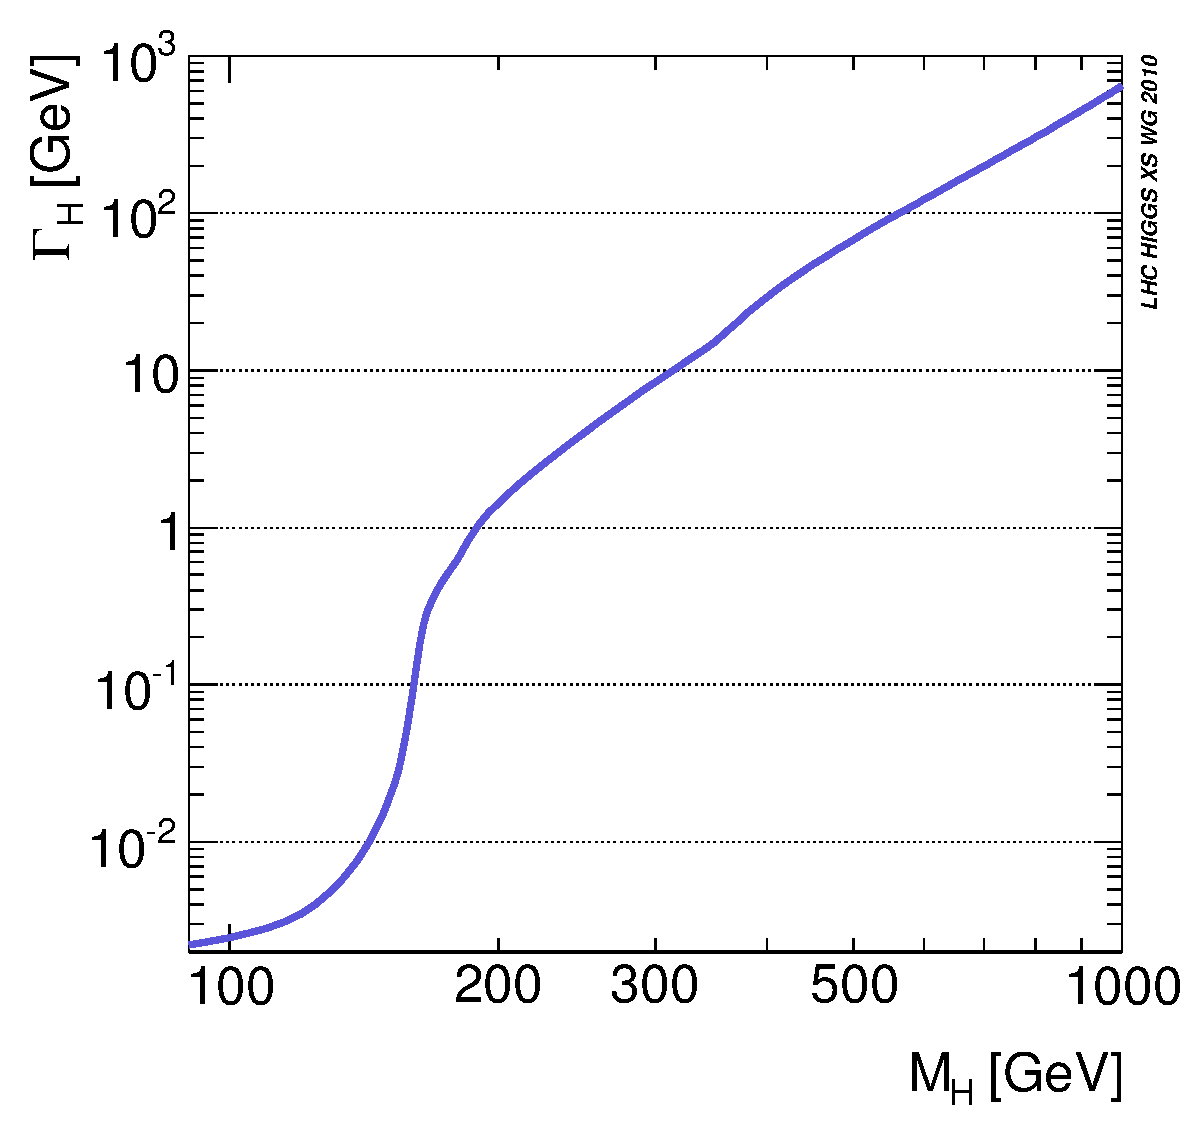
\includegraphics[width=0.7\textwidth]{images/width.pdf}
\caption{Total decay width of the SM Higgs boson as a function of $m_\mathrm{H}$.}\label{fig:width}
\end{figure}

Differential cross section measurements have also been performed by both experiments in the bosonic channels, $\gamma\gamma$, ZZ and $\mathrm{W^+W^-}$ (the latter is presented in Chapter~\ref{chap4} of this work), showing agreement with the SM-based theoretical predictions.


\cleardoublepage
\chapter{The CMS experiment at the LHC}\label{chap2}

\section{The Large Hadron Collider}
%%%%%%%%%%%%%%%%%%%%%%%%%%%%%%%%%%%%%%%%%
\label{sec:LHC}

The LHC~\cite{Pettersson:291782,Bruning:782076,Bruning:815187,Benedikt:823808} at CERN, officially inaugurated on $21^\mathrm{st}$ October 2008, is the largest and most powerful hadron collider ever built. Installed in the underground tunnel which hosted the Large Electron Positron Collider (LEP)~\cite{LEPreport1,LEPreport2,Wyss:314187}, the leptonic accelerator in operation until $2^\mathrm{nd}$ November 2000, the LHC accelerator has the shape of a circle with a length of about 27 km and is located underground at a depht varying between 50\,m to 175\,m, straddling the Franco-Swiss border near Geneva. It is designed to collide two 7\TeV counter-circulating beams of protons resulting in a centre-of-mass energy of 14\TeV, or two beams of heavy ions, in particular lead nuclei at an energy of 2.76\TeV/nucleon in the center-of-mass frame.

The transition from a leptonic collider to a hadronic collider entailed the following
advantages: first, it has been possible to build a machine that having the same size of the previous one (and therefore accommodated in the same LEP tunnel, substantially reducing the cost and time of construction), could reach a higher energy in the centre-of-mass frame. This is due to the much lower amount of energy loss through synchrotron radiation emitted by the accelerated particles, that is proportional to the fourth power of the ratio $E/m$ between their energy and their mass. Secondly, the composite structure of protons compared to the elementary structure of electrons allows LHC to be able to simultaneously access a wider energy spectrum, despite the production of many low energies particles
in a complex environment. This is a particularly important feature for a machine dedicated to the discovery of ``new'' physics.

\begin{figure}[htb]
\centering
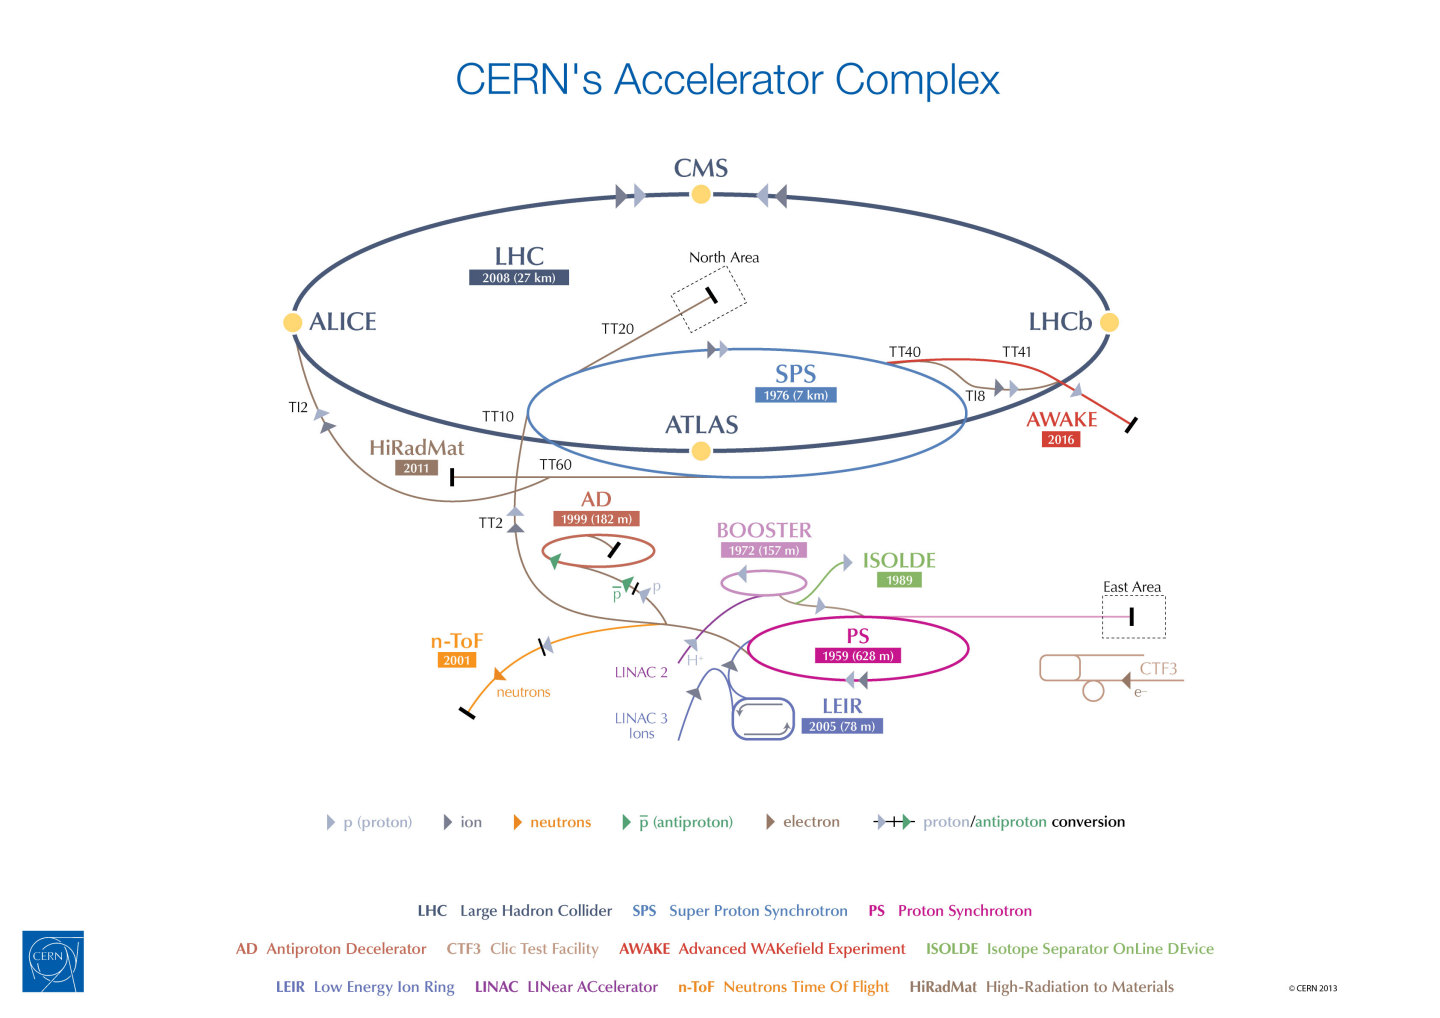
\includegraphics[width=\textwidth]{images/LHC.jpg}
\caption{Schematic description of the accelerator complex installed at CERN.}\label{fig:LHC}
\end{figure}

In Fig.~\ref{fig:LHC} a schematic description of the accelerator complex installed at CERN is shown.
The acceleration is performed in several stages~\cite{Benedikt:823808}. The protons source is a \emph{Duoplasmatron}: the protons are obtained by removing electrons from a source of hydrogen gas and then sent to the LINAC2, a 36\,m long linear accelerator which generates a pulsed beam with an energy of 50\MeV using Radio Frequency Quadrupoles (RFQ) and focusing quadrupole magnets. The beam is subsequently sent to the Proton Synchrotron Booster (PSB), a circular accelerator consisting of four superimposed synchrotron rings with a circumference of about 160\,m, which increases the proton energy up to $1.4$\GeV. Then, protons are injected into the Proton Synchrotron (PS), a single synchrotron ring with a circumference of about 600\,m where the energy is increased to 25\GeV. The sequential combination of these two synchrotrons also allows to create a series of protons bunches
interspersed by 25\,ns as required for the correct operation of LHC. The final proton injection stage is the Super Proton Synchrotron (SPS), a synchrotron with a circumference of approximately 7\,km where protons reach an energy value of 450\GeV. Subsequently, protons are extracted and injected into the LHC ring via two transmission lines, to generate two beams running in opposite directions in two parallel pipes and which are accelerated up to the energy of interest. In the two pipes an ultrahigh vacuum condition is maintained (about $10^{-10}$\,Torr) to avoid the spurious proton interactions with the gas remnants. At full intensity, each proton beam consists of 2808 bunches and each bunch contains around $10^{11}$ protons. The beams are squeezed and collide for a length of about 130\,m at four interaction points where the four main experiments (ALICE, ATLAS, CMS and LHCb) are placed:
\begin{itemize}
\item CMS (Compact Muon Solenoid)~\cite{Chatrchyan:2008aa} and ATLAS (A Toroidal LHC ApparatuS)~\cite{Aad:2008zzm} are two general-purpose detectors designed to investigate the largest possible spectrum of physics. In particular, they have been devoted to the detection of particles produced by a Higgs boson decay and to look for any evidence of possible new physics. The use of two detectors chasing the same objectives but designed independently is crucial for a cross-check of any possible new discovery;
\item LHCb (LHC beauty)~\cite{Alves:2008zz} is an experiment primarily designed to study CP (combined Charge conjugation and Parity symmetry) violation in electroweak interactions and to study asymmetries between matter and antimatter through the analysis of rare decays of hadrons containing b quarks. The detector is also able to perform measurements in the forward region, at small polar angles with respect to the beam line;
\item ALICE (A Large Ion Collider Experiment)~\cite{Aamodt:2008zz} is an experiment studying heavy ions collisions, through the production of a new state of matter called quark-gluon plasma.
\end{itemize}

Two other smaller experiments are located along the circumference of the LHC accelerator, TOTEM and LHCf, which focus on particles emitted in the forward direction. TOTEM (TOTal Elastic and diffractive cross section Measurement)~\cite{Anelli:2008zza} measures the proton-proton interaction cross section and accurately monitors the luminosity of the LHC using detectors positioned on either side of the CMS interaction point. LHCf (LHC forward)~\cite{Adriani:2008zz} is made up of two detectors which sit along the LHC beamline, at 140\,m either side of the ATLAS collision point. It makes use of neutral particles thrown forward by LHC collisions as a source to simulate the interaction with the atmosphere of very high energy cosmic rays (between $10^{17}$\TeV and $10^{20}$\TeV) in laboratory conditions.

A series of about 1200 magnetic dipoles bend the beams along the accelerator ring. They are located along the ``arc'' structures of the circumference. The ring, in fact, can be subdivided into octants, with eight curve regions (the ``arcs'') separated by rectilinear regions. In these straight regions, instead, almost 400 focusing and defocusing quadrupoles are located, which maintain the beam stable along the orbit, and some other small multipolar magnets (sextupoles and octupoles) are used to make additional minor corrections to the beam direction. A radio frequency acceleration system, consisting of 16 superconducting radio-frequency resonant cavities, is used to increase the proton energy by 0.5\MeV with each beam revolution. The 7\TeV per-beam-energy limit on the LHC is not determined by the electric field generated by the radiofrequency cavity but by the magnetic field necessary to maintain the protons in orbit, given the current technology for the superconducting magnets, which is about 5.4\,T on average.

One of the most important parameters of an accelerator is the instantaneous luminosity $\mathcal{L}$, which gives a measure of the rate of events one can expect given the process cross section. In fact, for a given physics process with cross section $\sigma$, producing $N$ events for unit of time, the instantaneous luminosity is defined by the following equation:
\begin{equation}
N = \sigma\mathcal{L} \quad .
\end{equation}
The LHC design luminosity is $\mathcal{L} = 10^{34} \mathrm{cm^{-2} s^{-1}}$, leading to around 1 billion proton interactions per second.

The instantaneous luminosity is a parameter which depends on the construction characteristics of the accelerator, and can be expressed by the following approximated formula:
\begin{equation}
\mathcal{L} = f\frac{n_1 n_2}{4\pi\sigma_x\sigma_y} \quad ,
\end{equation}
where $n_1$ and $n_2$ are the number of particles contained in the two bunches colliding at a frequency $f$, and $\sigma_x$ and $\sigma_y$ are the beam sizes in the transverse plane. At LHC, the bunches collide with $f=40$\,MHz and the transverse size of the beam can be squeezed down to around $15$\,\micron.
Then, the integrated luminosity $L$ is defined as the time integral of the instantaneous luminosity:
\begin{equation}
L = \int \mathcal{L} dt \quad .
\end{equation}
The main parameters of the LHC machine are listed in Table~\ref{tab:LHCparams}.

\begin{table}[htb]
\caption{LHC technical parameters for proton-proton collisions.}\label{tab:LHCparams}
\centering
\begin{tabular}{lc}
\toprule
{\bfseries Parameter} & {\bfseries Value}\\
\midrule
Maximum dipole magnetic field & 8.33\,T \\
Dipole operating temperature & 1.9\,K \\
\midrule
Beam energy at injection & 450\GeV \\
Beam energy at collision (nominal) & 7\TeV \\
Beam energy at collision (2012) & 4\TeV \\
Beam energy at collision (2015--2016) & 6.5\TeV \\
\midrule
Maximum instantaneous luminosity (nominal) & $10^{34}\,\mathrm{cm^{-2}s^{-1}}$ \\
Maximum instantaneous luminosity (2012) & $7.7\cdot10^{33}\,\mathrm{cm^{-2}s^{-1}}$ \\
Maximum instantaneous luminosity (2015--2016) & $1.2\cdot10^{34}\,\mathrm{cm^{-2}s^{-1}}$ \\
\midrule
Number of bunches per proton beam (nominal) & 2808 \\
Number of bunches per proton beam (2012) & 1380 \\
Number of bunches per proton beam (2015--2016) & 2220 \\
Maximum number of protons per bunch & $1.69\cdot10^{11}$ \\
\midrule
Bunch separation in time (nominal) & 25\,\ns \\ 
Bunch separation in time (2012) & 50\,\ns \\ 
Bunch separation in time (2015--2016) & 25\,\ns \\
Collision frequency (nominal) & 40\,MHz \\ 
Collision frequency (2012) & 20\,MHz \\ 
Collision frequency (2015--2016) & 40\,MHz \\
\midrule
Energy loss per turn at 14\TeV & 7\,keV \\
\bottomrule
\end{tabular}
\end{table}

The LHC started to be operative in September 2008 but, due to a faulty interconnection between two magnets which caused a helium leakage in the tunnel, the operation was stopped and restarted in March 2010. During 2010 and 2011 LHC ran successfully and provided proton-proton collisions at a centre-of-mass energy of 7\TeV, delivering a total integrated luminosity of about 6.1\ifb. The encouraging results in the Higgs boson search provided by the ATLAS and CMS Collaborations led to the decision of extending the data taking period to the end of 2012, and to increase the center-of-mass energy up to 8\TeV. During 2012, LHC delivered to the experiments an integrated luminosity of 23.3\ifb. After the first long shutdown (LS1), a two years period started in the early 2013 where the LHC operation stopped for maintenance and upgrade, the LHC started again delivering proton-proton collisions on $3^\mathrm{rd}$ June 2015, at the new record centre-of-mass energy of 13\TeV. During the 2015 the LHC delivered an integrated luminosity of 4.2\ifb. Nowadays, LHC is still colliding bunches of protons at $\sqrt{s}=13$\TeV, reaching unprecedented instantaneous luminosities and delivering a total integrated luminosity of 31\ifb. The cumulative delivered luminosity versus time for the different LHC data taking periods is shown in Fig.~\ref{fig:LHClumi}.

\begin{figure}[htb]
\centering
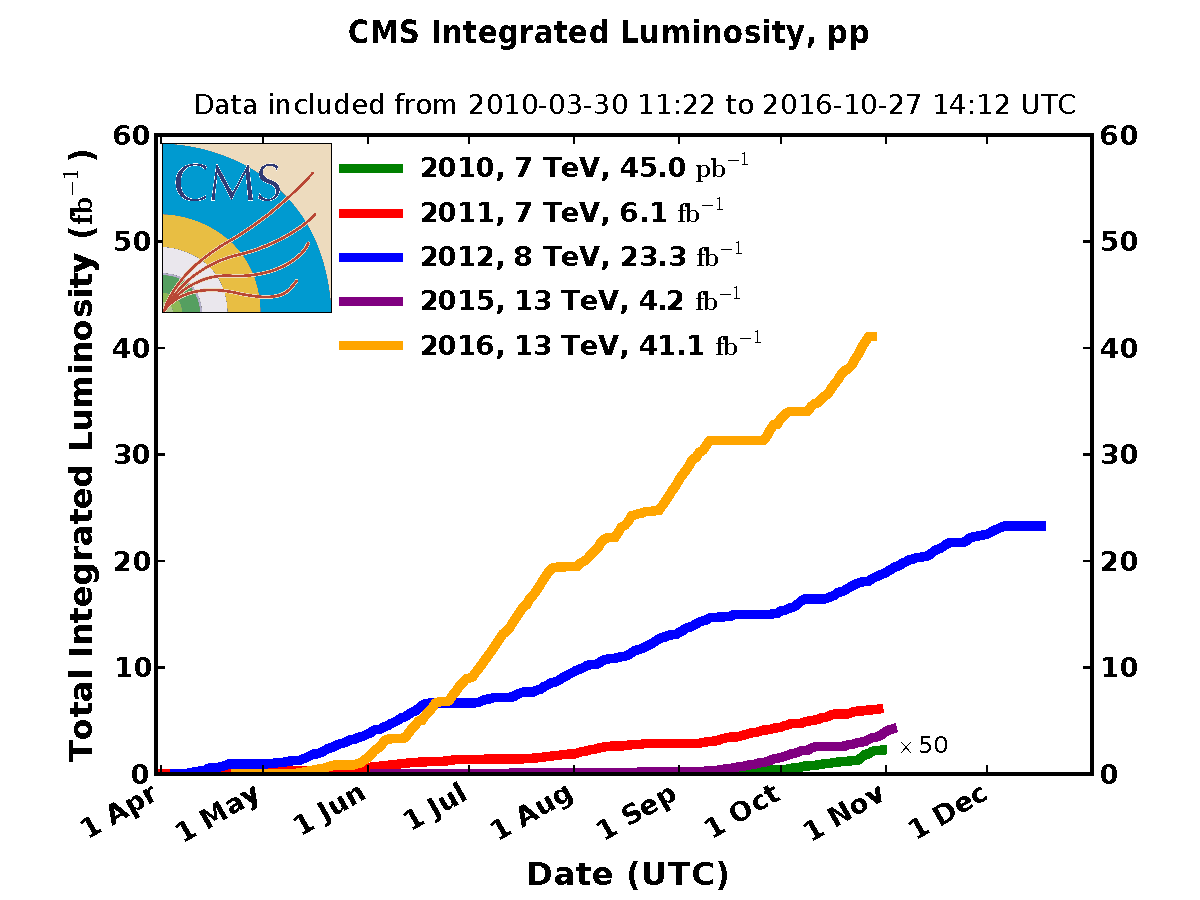
\includegraphics[width=0.7\textwidth]{images/LHClumi.pdf}
\caption{Cumulative luminosity versus day delivered to CMS during proton-proton collisions.}\label{fig:LHClumi}
\end{figure}

As the instantaneous luminosity increases, the probability of multiple proton-proton interactions to occur in a single bunch crossing grows higher as well. In this instance, the main goal is the identification and reconstruction of a single primary collision where the physics event of interest occurs among the background of the additional proton-proton interactions. Such backgrounds are due to processes occurring with very high probability, like the production of low-\pt jets. These additional collisions are known as pile up (PU). During the LHC current run the average number of pile up events is 23, with some event exhibiting over 45 pile up collisions. 











\section{The CMS experiment}
%%%%%%%%%%%%%%%%%%%%%%%%%%%%%%%%%%%%%%%%%
\label{sec:CMS}

\section{The CMS trigger system}
%%%%%%%%%%%%%%%%%%%%%%%%%%%%%%%%%%
\label{sec:Trigger}

The LHC can provide proton-proton interactions at a crossing frequency of 40\,MHz and, for each bunch crossing, several collisions can occur (approximately 20 at the nominal instantaneous luminosity). Since it is impossible to store and process the large amount of data associated with the resulting large number of events, a drastic rate reduction has to be achieved. In fact, the speed at which data can be written to mass storage is limited and, moreover, the vast majority of produced events is not interesting for physics analyses, because it involves low transverse momentum interactions (also called \emph{minimum bias events}). The task of reducing this rate is accomplished by the CMS trigger system, which represents the first step of the physics event selection. CMS makes use of a two-stage trigger system, consisting of a \emph{Level-1} trigger (L1)~\cite{Dasu:2000ge} and a \emph{High Level Trigger} (HLT)~\cite{Cittolin:578006}.

Level-1 trigger runs on dedicated processors, and accesses coarse level granularity information from calorimetry and muon system. A L1 trigger decision has to be taken for each bunch crossing within $3.2\,$\textmu s. Its task is to reduce the data flow from 40\,MHz to about 100\,kHz.

The High Level Trigger is responsible for reducing the L1 output rate down to a maximum rate of the order of 1\,kHz. The HLT code runs on a farm of commercial processors and can access the full granularity information of all the subdetectors.

The main characteristics of the CMS trigger system are described in the following.

%%%%%%%%%%%%%%%%%%%%%%%%%%%%%%%%%%%%%%%%%%%%%%%%%%%%%%%%%
\subsection{The Level-1 trigger}

The L1 trigger is responsible for the identification of electrons, muons, photons, jets and missing transverse energy. It is required to have a high and carefully understood efficiency. Its output rate and speed are limited by readout electronics and performance of the data
acquisition (DAQ) system~\cite{Cittolin:578006}. It consists of three main subsystems:
\begin{itemize}
\item L1 Calorimeter Trigger;
\item L1 Muon Trigger;
\item L1 Global Trigger.
\end{itemize}
The L1 Global Trigger is responsible for combining the output of L1 Calorimeter
Trigger and L1 Muon Trigger and for making the decision to either retain the event or discard it. The organization of CMS L1 Trigger is schematically summarized in Fig.~\ref{fig:trigL1}.
\begin{figure}[htb]
\centering
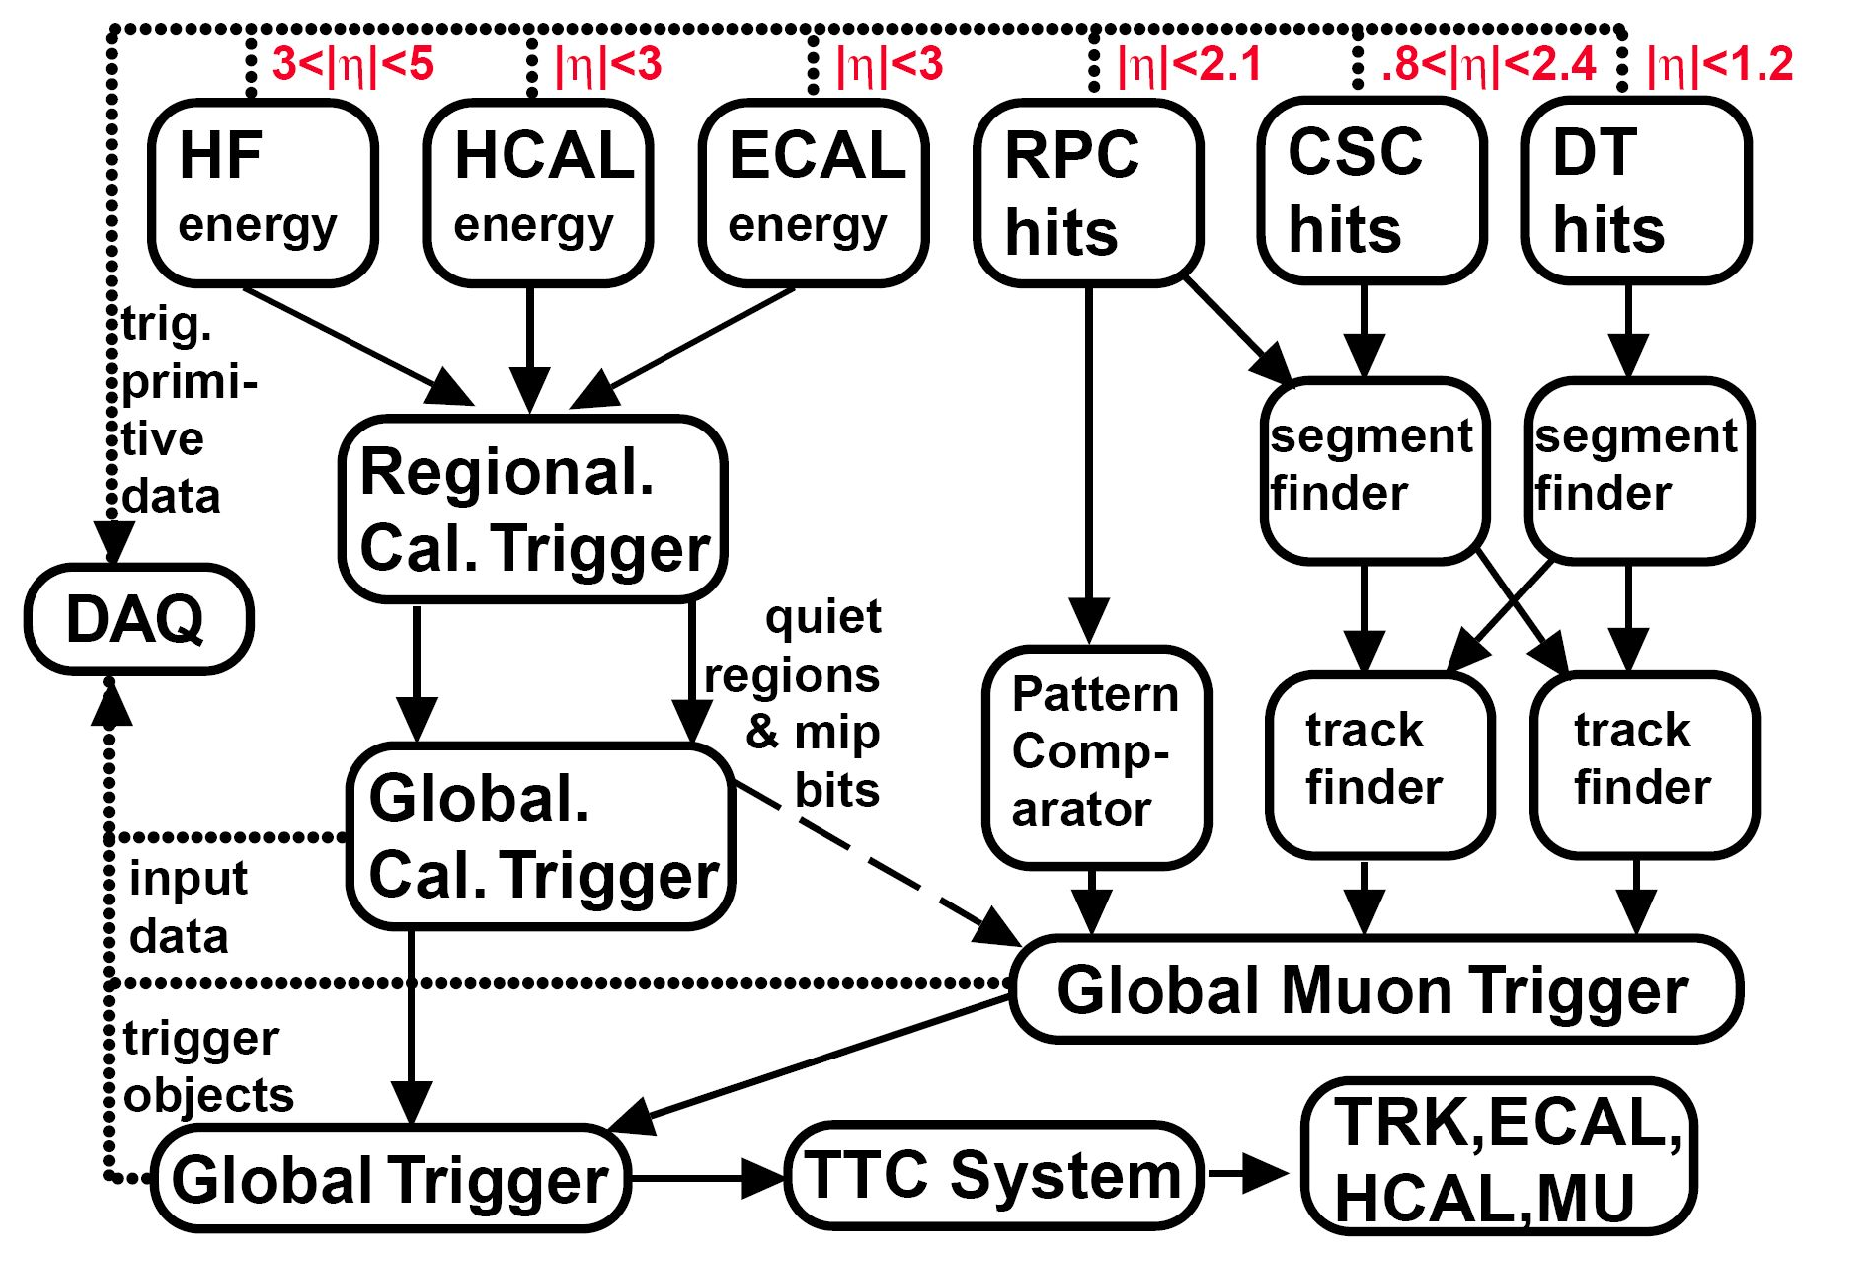
\includegraphics[width=0.7\textwidth]{images/trigL1.png}
\caption{Schematic representation of the Level-1 trigger components.}\label{fig:trigL1}
\end{figure}

\subsubsection{L1 Calorimeter Trigger}

The input for the L1 Calorimeter Trigger are calorimeter towers, which are clusters of signals collected both from ECAL and HCAL. Towers are calculated by calorimeter high level readout circuits, called Trigger Primitive Generators. The Regional Calorimeter Trigger identifies electron, photon, $\tau$ and jet candidates together with their transverse energy and sends the information to the Global Calorimeter Trigger. The Global Calorimeter Trigger sorts the candidates according to their transverse energy and sends the first four objects to the L1 Global Trigger.

\subsubsection{L1 Muon Trigger}

The L1 Muon Trigger is actually a composite system istelf: information from RPC, CSC and DT specific triggers are combined in the so called L1 Global Muon Trigger. 

The RPC trigger electronics builds Track Segments, gives an estimate of their \pt and sends these segments to the Global Muon Trigger. It also provides the CSC logic unit with information to solve hit position ambiguities in case of two or more muon tracks crossing the same CSC chamber. 

The CSC trigger builds Local Charged Tracks (LCT), that are track segments made out of the cathode strips only, and assign a \pt value and a quality flag to the LCTs. The best three LCTs in each sector of nine CSC chambers are passed to the CSC Track Finder, which uses the full CSC information to build tracks, assigns them a \pt and a quality flag and sends them to the Global Muon Trigger.

DTs are equipped with Track Identifier electronics, which is able to find groups of aligned hits in the four chambers of a superlayer. Those Track Segments are sent to the DT Track Correlator that tries to combine segments from two superlayers, measuring the $\phi$ angle. The best two segments are sent to the DT Track Finder that builds tracks and sends them to the Global Muon Trigger.

The Global Muon Trigger sorts the RPC, CSC and DT muon tracks and tries to combine them. The final set of muons is sorted according to the quality, and the best four tracks are passed to the L1 Global Trigger.

\subsubsection{L1 Global Trigger}

The L1 Global Trigger is responsible for collecting objects created from the Calorimeter and Muon Triggers and making a decision whether to retain the event or not. In case the event is accepted the decision is sent to the Timing Trigger and Control System, which command the readout of the remaining subsystems.

In order to take the decision, the L1 Global Trigger sorts the ranked objects produced by calorimetry and muon system and checks if at least one of the thresholds in the L1 trigger table is passed.

%%%%%%%%%%%%%%%%%%%%%%%%%%%%%%%%%%%%%%%%%%%%%%%%%%%%%%%%%
\subsection{The High Level Trigger}

The HLT is designed to reduce the L1 output rate down to about 1000\,$\mathrm{events/s}$, which is the amount that will be written to mass storage. HLT code runs on commercial processors and performs reconstruction using the information from all subdetectors. Events passing
the HLT are stored on local disks or in CMS Tier 0\footnote{The Worldwide LHC Computing Grid (WLCG) is composed of four levels, or ``Tiers'', identified with numbers 0, 1, 2 and 3. Each Tier is made up of several computer centres and provides a specific set of services; they process, store and analyse all the data from the LHC. Tier 0 is the CERN Data Centre. All of the data from the LHC pass through this central hub. Tier 0 distributes the raw data and the reconstructed output to Tier 1's, and reprocesses data when the LHC is not running.}. 

Data read from subdetectors are assembled by a builder unit and then assigned to a switching network that dispatches events to the processor farm. The CMS switching network has a bandwidth of 1 Tbit/s. This simple design ensures maximum flexibility to the system, the only limitation being the total bandwidth and the number of processors. The system can be easily upgraded adding new processors or replacing the existing ones with faster processors as they become available. Since the algorithms have a fully software implementation, improvements to the algorithms can be easily implemented and do not require any hardware intervention.

Event by event, the HLT code is run on a single processor, and the time available to make a decision is about 300 ms. The real time nature of this selection imposes several constraints on the resources an algorithm can use. The reliability of HLT algorithms is of capital importance, because events not selected by the HLT are lost. In order to efficiently process events, the HLT code has to be able to quickly reject not interesting events; computationally expensive algorithms must be run only on good candidates for interesting events. In order to cope with this requirement the HLT code is organized
in a virtually layered structure:
\begin{itemize}
\item Level 2: uses only complete muon and calorimetry information;
\item Level 2.5: uses also the pixel information;
\item Level 3: makes use of the full information from all the tracking detectors.
\end{itemize}
Each step reduces the number of events to be processed in the following step. The most computationally expensive tasks are executed in the Level 3; time consuming algorithms such as track reconstruction are only executed in the region of interest. Besides, since the ultimate precision is not required at HLT level, track reconstruction is performed on a limited set of hits, and is stopped once the required resolution is achieved.









\section{Event reconstruction and particle identification}
%%%%%%%%%%%%%%%%%%%%%%%%%%%%%%%%%%%%%%%%%%%%%%%%%%%%%%
\label{sec:Objects}

In CMS, the physics object reconstruction and identification is based on standard algorithms developed by the collaboration and used by all the physics analyses. In this section, the techniques used for the reconstruction and identification of the physics objects of interest for \hwwllnn analyses are described.

\subsection{The Particle Flow technique}

The Particle Flow (PF) event reconstruction technique~\cite{CMS-PAS-PFT-09-001} aims at the reconstruction and identification of all the stable particles in the event, i.e. electrons, muons, photons, charged and neutral hadrons, with a thorough combination of the information from all CMS sub-detectors, in order to determine their energy, direction and type. These individual particles are then used, for example, to build jets, to measure the missing transverse energy \MET, to reconstruct the $\tau$ from their decay products, to quantify the charged lepton isolation and to tag b-jets.

The CMS detector is well suited for this purpose. Indeed, the presence of a large internal silicon tracker immersed in an intense solenoidal magnetic field allows the reconstruction of charged particles with high efficiency and small fake rate, and provides a high precision measurement of the particle \pt down to about $150\,\MeV$, for $|\eta|\leq2.6$. The high granularity of the ECAL calorimeter is the additional key element for the feasibility of the PF technique, allowing the reconstruction of photons and electrons with high energy resolution.

The first step of the PF technique consists in the reconstruction of the basic elements from the various sub-detectors, such as charged-particle tracks, calorimeter clusters and muon tracks. These elements, which are provided by the sub-detectors with high efficiency an low fake rate, are then connected together with a link algorithm.

The good performance of the tracking system are achieved by means of an iterative tracking strategy~\cite{Chatrchyan:2014fea}, based on the Kalman Filter algorithm~\cite{Billoir:1990we}. The basic idea of iterative tracking is that initial iterations search for tracks that are easiest to find, e.g. high \pt tracks produced near the interaction region. After each iteration, hits associated to reconstructed tracks are removed from the hit collection, thereby reducing the combinatorial complexity and simplifying the subsequent iterations, which aim at finding more complicated set of tracks, e.g. low \pt or displaced tracks. The \emph{Iteration 0}, where the majority of tracks are reconstructed, is designed to identify prompt tracks with $\pt>0.8$\,\GeV that have three hits in the three layers of the pixel detector. \emph{Iteration 1} is used to recover prompt tracks that have only two pixel hits. \emph{Iteration 2} aims at finding low-\pt prompt tracks while \emph{Iterations 3--5} are intended to find tracks that originate outside the collision point, i.e. tracks produced by a secondary vertex, and to recover undetected tracks in the previous iterations. Each iteration proceeds according to four steps:
\begin{itemize}
\item \emph{seeding}: initial track candidates are obtained using 2 or 3 hits in the innermost layers (these proto-tracks are called seeds);
\item \emph{pattern recognition}: this step is based on Kalman Filter and searches for hits in the outer layers that could be associated to the initial track candidate, reconstructing the particle trajectory;
\item \emph{track fitting}: in this step a fit of the trajectory is performed, using its associated hits and providing an estimate of the track parameters (\pt, $\eta$, $\phi$, charge, etc.);
\item \emph{selection}: finally tracks are selected based on quality requirements.
\end{itemize}

The high detection efficiency of the calorimeters is based on a specific calorimeter clustering algorithm, which is performed separately in each sub-detector. The algorithm is based on three steps: in the first step, ``cluster seeds'' are identified as local calorimeter cells with an energy deposit above a given threshold. Then, ``topological clusters'' are grown from the seeds by gathering cells with at least one side in common with a cell already in the cluster, and with an energy above a given threshold. A topological cluster usually gives rise to many ``particle flow clusters'' as seeds, which are identified sharing the energy of each cell among the particle flow clusters, thereby allowing the determination of the particle flow cluster energy and position.

These elements are then connected to each other using a link algorithm, which identifies blocks of elements that are topologically compatible. For example, a charged-particle track is linked to a calorimeter particle flow cluster if the extrapolated position from the track to the calorimeter is compatible with the cluster boundaries. From these blocks, PF candidates are identified according to the following order:
\begin{itemize}
\item Muons: a \emph{global muon} gives rise to a \emph{PF muon} if its combined \pt measurement is compatible within 3 standard deviation with the one provided by the sole tracker. The corresponding track is removed from the block;
\item Electrons: electrons tend to give rise to short tracks, and to lose energy by Bremsstrahlung in the tracker layers on their way to the calorimeter. The link between a charged-particle track (refitted with the Gaussian-Sum Filter (GSF)~\cite{Adam:815410}) and one or more ECAL clusters identifies a \emph{PF electron}. After the identification, the corresponding tracks and clusters are removed from the block.
\item Charged hadrons: the remaining tracks give rise to \emph{PF charged hadrons}. Tracks can be linked to ECAL and HCAL clusters, and the energy is determined taking into account information from calorimeters;
\item Photons and neutral hadrons: ECAL clusters not linked with tracks give rise to \emph{PF photons}, while the remaining HCAL clusters are identified as \emph{PF neutral hadrons}.
\end{itemize}
After the identification of all PF candidates in the event, \emph{PF jets} are clustered as described in Sec.~\ref{chap2:jets}. The last step is the reconstruction of the \emph{PF \ptmiss}, which is given by:

\begin{equation} 
\ptmiss = - \sum_{\mathrm{PF\,obj}} \vec{p}_\mathrm{T}^\mathrm{\,PF\,obj} \quad,
\end{equation}

where the sum extends over all the PF objects. The \MET is defined as the modulus of \ptmiss.

\subsection{Leptons reconstruction and identification}

\subsubsection{Muon reconstruction and identification}
Muons produced at the collision point can go through the entire detector with a negligible energy loss, thus reaching the detector outermost part where the muon chambers are installed (see Sec.~\ref{sec:muonsyst}). Muons interact through ionization with the layers of the silicon tracker, which is able to reconstruct their tracks (\emph{tracker track}). The muon tracks are also reconstructed using the muon system (\emph{standalone muon track}). Based on these objects, two reconstruction approaches are used~\cite{Chatrchyan:2012xi}: in the first method (outside-in), for each standalone muon tracks a tracker track is searched for by extrapolating the two tracks to a common surface. If a match is found, the hits associated to the two tracks are fitted together giving rise to a \emph{Global Muon}. The second approach (inside-out) consists in considering all tracker tracks with $\pt > 0.5$\,\GeV as potential muon candidates and are extrapolated to the muon system taking into account the magnetic field, the expected energy losses and the multiple scattering in the detector material. If at least one muon segment (a short track stub made of DT or CSC hits) matches the extrapolated tracks, the corresponding tracker track is identified as a \emph{Tracker Muon}.

The matching with the muon system improves significantly the muon \pt resolution that can be obtained from the tracker only, especially in the region with $\pt > 200$\GeV, as shown in Fig.~\ref{fig:muptres}. 
\begin{figure}[htb]
\centering
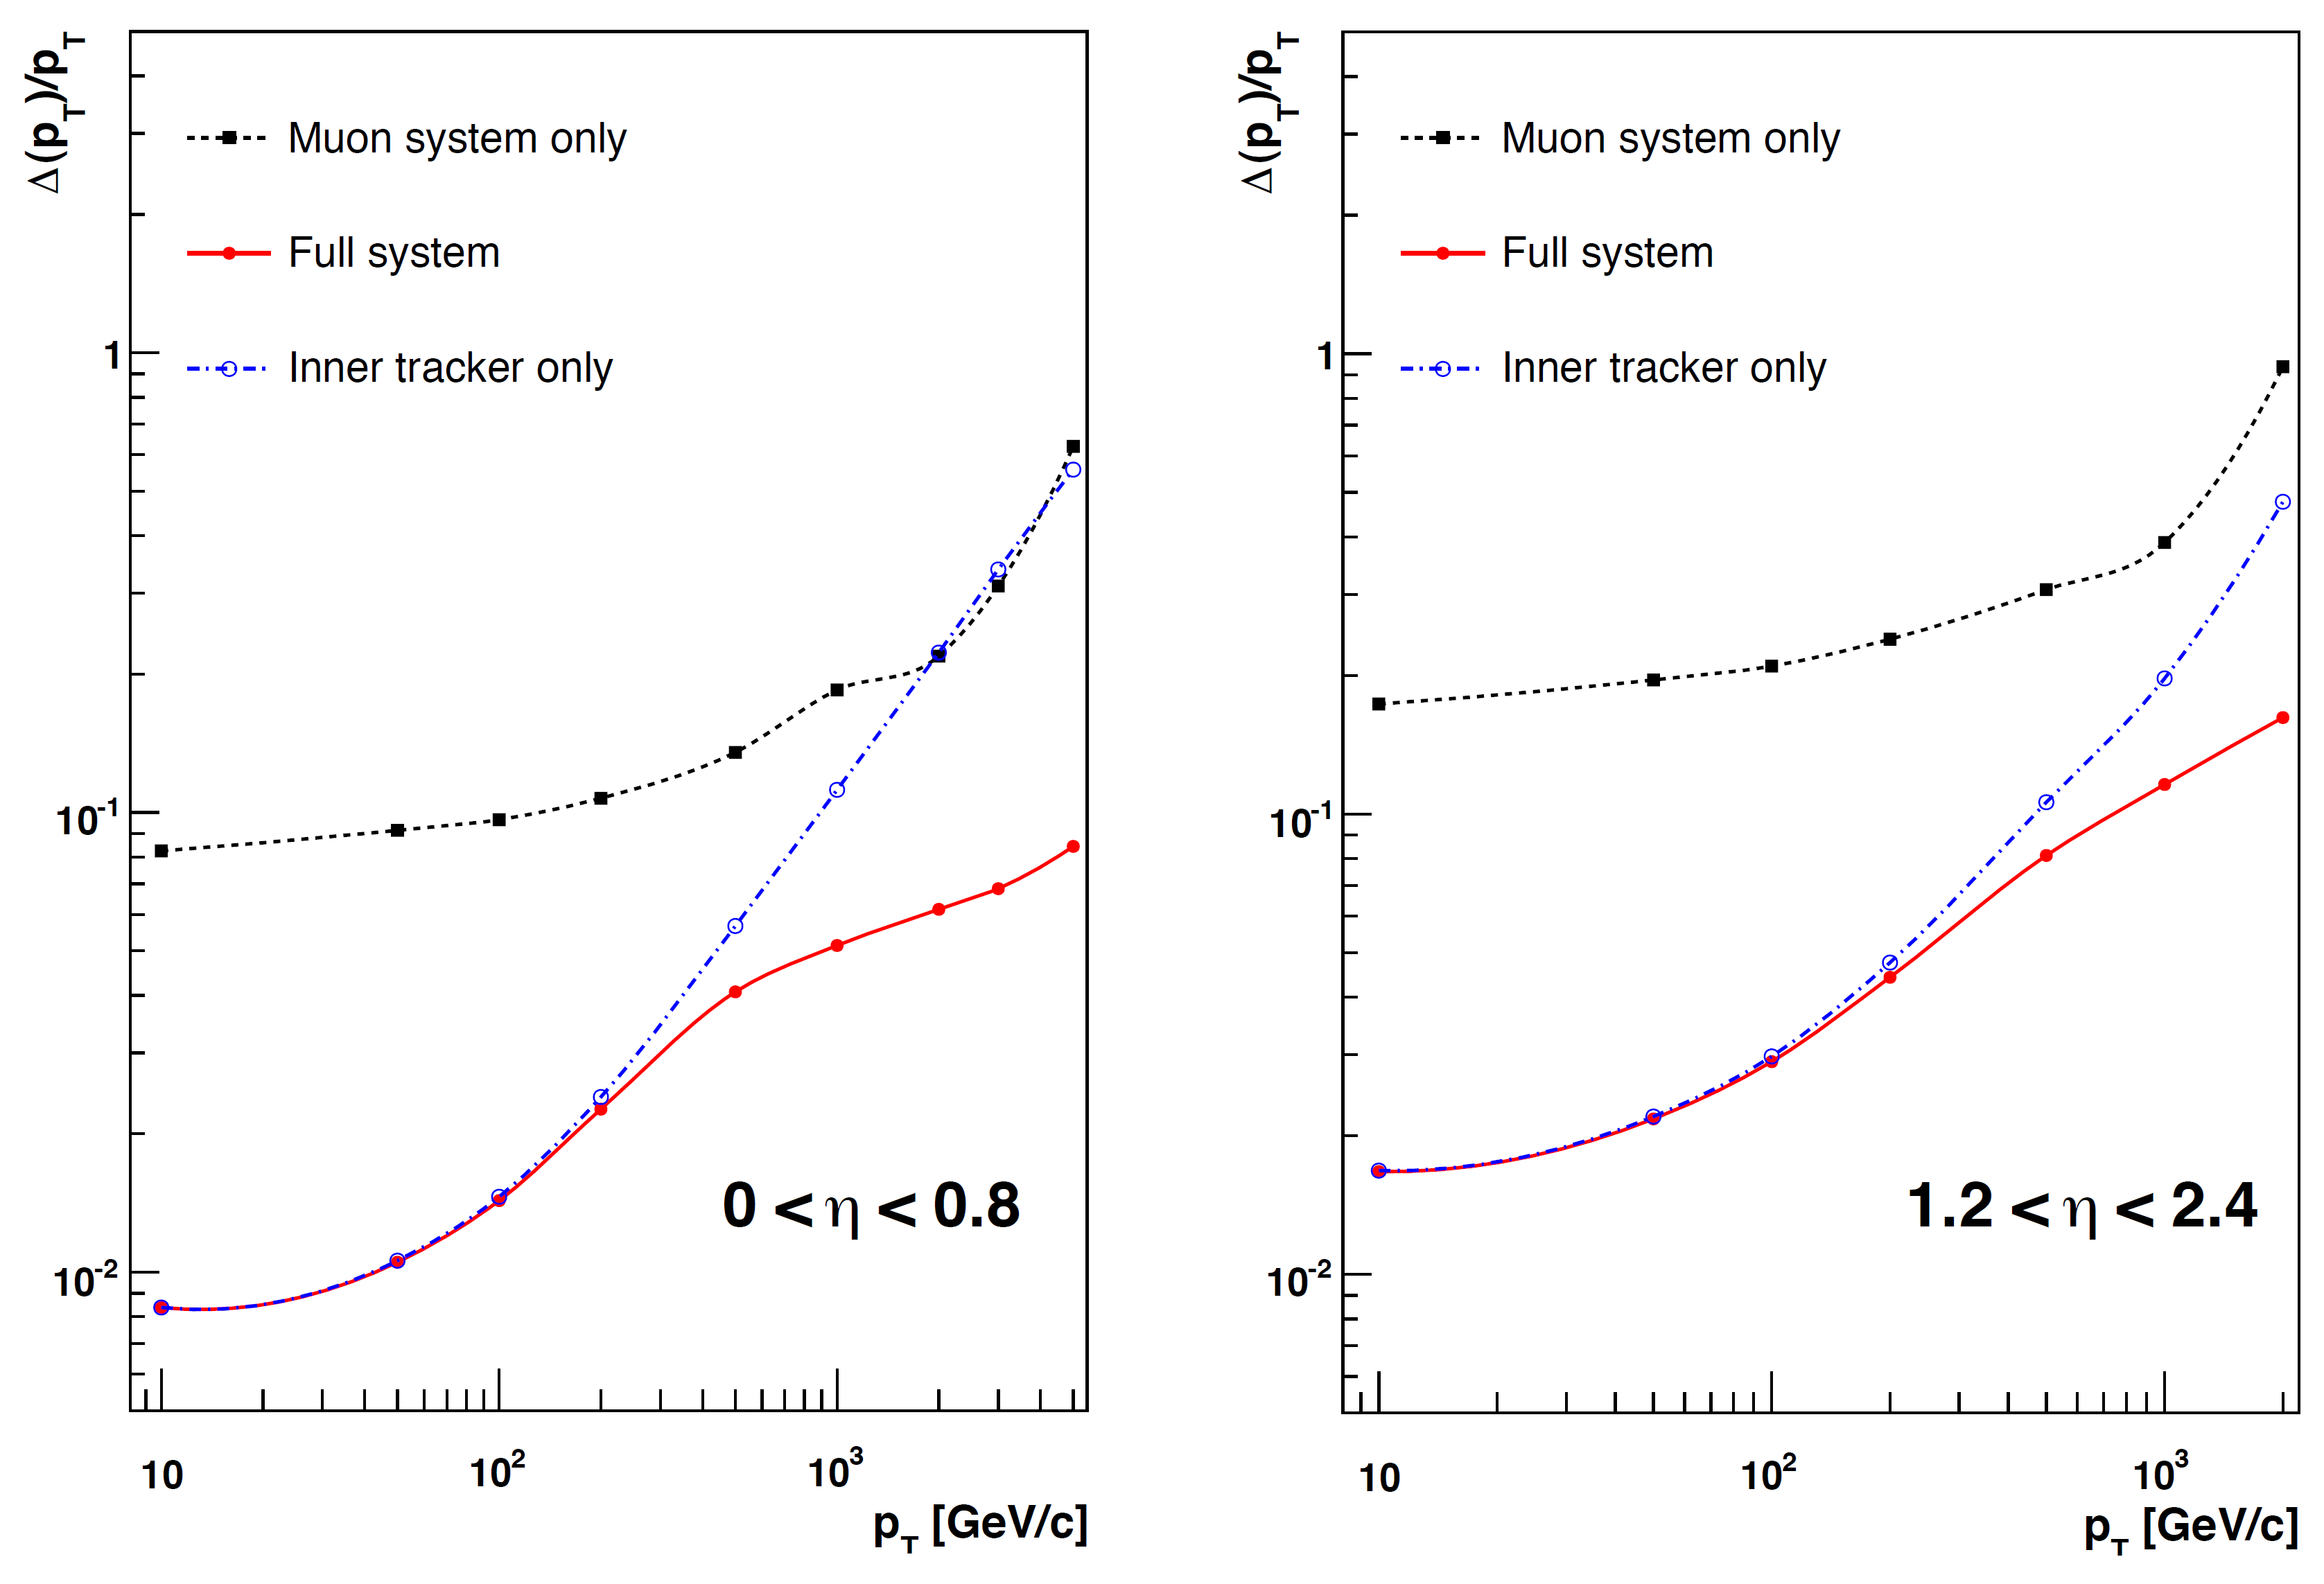
\includegraphics[width=0.6\textwidth]{images/muptres.png}
\caption{Muon \pt resolution as a function of the muon \pt in the barrel (left) and in the endcap (right) regions. The resolution is provided for the measurement using the tracking system or the muon system only, as well as for the combination of the two methods.}\label{fig:muptrese}
\end{figure}

Depending on the physics analysis, different muon definitions can be used by changing the selection on the muon identification variables, hence balancing between the muon identification efficiency and purity. The most widely used definition in physics analyses is the so-called \emph{Tight muon selection}\footnote{Small variations with respect to this baseline definition are adopted by the specific analyses.}. This selection requires the muon candidate to be reconstructed as a Global Muon and identified by the PF algorithm. The fit of the global track, which is required to include muon segments in at least two muon stations (this implies that the muon is also reconstructed as a Tracker Muon), must have a $\chi^2/d.o.f.$ less than 10 and use more than 10 inner tracker hits. The transverse impact parameter with respect to the primary vertex is required to be $|d_{xy}|<2$\,mm, significantly reducing the rate of muons from decays in flight, i.e. non prompt muons. The requirements defining the Tight Muon identification are summarized in Table~\ref{tab:tightmuon}.

\begin{table}[htb]
\caption{Summary of the muon identification variables and the corresponding selections commonly used by physics analyses.}\label{tab:tightmuon}
\centering
\begin{tabular}{lc}
\toprule \\
Observable & Cut \\
\midrule \\
Is Global Muon & true \\
Is PF muon & true \\
Tracker layers with valid hits & $>5$ \\
Number of valid pixel hits & $>0$ \\
Number of valid muon hits & $>0$ \\
Number of matched muon stations & $>1$ \\
$\chi^2/d.o.f.$ & $<10$ \\
$d_{xy}(PV)$ & $< 0.2$\,cm \\
$d_{z}(PV)$ & $< 0.5$\,cm \\
\bottomrule \\
\end{tabular}
\end{table}

Another selection which is optimised for low-\pt muons coming from in flight decays is called \emph{Soft Muon selection}. This selection requires the muon to be reconstructed as a Tracker Muon with loose additional cuts on the transverse and longitudinal impact parameters. This selection is commonly used to identify muons coming from B hadron decays.

\subsubsection{Muon isolation}
One of the most powerful requirements to select prompt muons, as the ones produced from W or Z boson decays, and to reject muons produced by decays in flight, is the isolation. Indeed, prompt muons are expected to be isolated in the event, differently to non prompt muons that are generally produced within jets and characterized by many nearby particles.

Muons commonly used to reconstruct the W or Z decays are thus required to pass an isolation requirement, which includes a pile up mitigation correction called ``$\Delta\beta$ correction''. This correction is needed to obtain a robust isolation definition that is less sensitive to the pile up contribution. Indeed, simultaneous interactions manifest themselves as a mean energy deposited over all the detector acceptance, which is not due to the particles produced in the primary events, thus spoiling the isolation measurement. The relative isolation variable, usually called \emph{PF relative isolation}, is defined as follows:

\begin{equation}\label{eq:isomu}
I^{rel}_{\Delta\beta} = \left[  \sum_{ChH}\pt + max\left(0, \sum_{NH}\pt + \sum_{Ph}\pt - 0.5\sum_{ChHPU}\pt    \right)  \right]/\pt^\mathrm{muon} \quad .
\end{equation}

The sums in Eq.~\eqref{eq:isomu} are performed in a cone of radius $\Delta R < 0.4$ around the muon direction. The $ChH$ subscript refers to charged hadrons, $NH$ to neutral hadrons, $Ph$ to photons and $ChHPU$ to charged hadrons not arising from the primary vertex.

The cut applied on the isolation variable is analysis dependent, but a common value is $I^{rel}_{\Delta\beta} < 0.15$.

A different isolation definition is called \emph{Tracker relative isolation}, $I^{rel}_{trk}$, which is calculated as the scalar sum of all the \pt of the tracker tracks reconstructed inside a cone of radius $\Delta R < 0.3$ centred on the muon track direction.

\subsubsection{Muon momentum scale and resolution}
The measurement of the muon \pt is sensitive to the alignment of the tracker and the muon chambers, to the material composition and distribution inside the detector and to the knowledge of the magnetic field produced by the solenoid. The imperfect knowledge of the magnetic field and the effect of the material distribution introduce a relative bias in the muon \pt that is generally independent on the \pt itself, while the effect of the alignment is known to produce a bias that increases linearly with the \pt.

Different methods are used to estimate the muon \pt scale and resolution effects and to determine the corresponding uncertainties, depending on the \pt range. At low and intermediate \pt ($< 100$\,\GeV), the di-muon events arising from the $J/\Psi$ and Z resonance decays are used to correct the \pt scale and to measure the \pt resolution. In the high \pt regime, the muon \pt scale and resolution are instead measured using cosmic ray muons. One of the methods that is commonly used in the intermediate \pt range is the \emph{MuScleFit} (Muon momentum Scale calibration Fit), which provides the muon \pt scale corrections by fitting the Z boson mass peak in data and simulation. These corrections are meant to recover the bias of the Z mass peak with respect to the $\eta$ and $\phi$ coordinates of the muon. After applying these corrections the relative \pt resolution, $\sigma(\pt)/\pt$), is measured as a function of $\eta$ and $\phi$ and is found to be on average of the order of 2\% in the barrel and up to 6\% in the endcaps, for muon \pt below 100\,\GeV.

\subsubsection{Electron reconstruction and identification}

The electron reconstruction is based on the combination of tracker and ECAL information. The reconstruction technique starts by measuring the energy deposits in ECAL by electrons, which form a ``supercluster''. A supercluster is a group of one or more ECAL clusters associated using an algorithm that takes into account the characteristic shape of the energy deposited by electrons emitting Bremsstrahlung radiation in the tracker material. The supercluster shape is characterized by a narrow width profile in the $\eta$ coordinate spread over the $\phi$ direction. The superclusters are matched to tracks, reconstructed in the tracker with the GSF algorithm, in order to obtain an electron candidate. An additional reconstruction method, described in details in Ref.~\cite{CMS-PAS-EGM-10-004}, is instead seeded by electron tracks reconstructed in the inner tracker layers.

Several strategies are used in CMS to identify prompt isolated electrons (characteristic of the signal processes of interest), and to separate them from background sources, mainly originating from photon conversions, jets misidentified as electrons, or electrons from semileptonic decays of b and c quarks. In order to achieve a good discrimination, several identification variables are used:
\begin{itemize}
\item $\Delta\eta_\mathrm{trk,SC}$ and $\Delta\phi_\mathrm{trk,SC}$: the variables measuring the spatial matching between the track and the supercluster in the $\eta$ and $\phi$ coordinates, respectively;
\item $\sigma_{i\eta,i\eta}$: a variable related to the calorimeter shower shape, measuring the width of the ECAL supercluster along the $\eta$ direction computed for all the crystals in the $5
\times 5$ block of crystals centred on the highest energy crystal of the seed supercluster;
\item $H/E$: the ratio between the energy deposited in the HCAL tower behind the ECAL seed and the supercluster seed energy;
\item $|1/E - 1/p|$: the difference of the inverse of energy $E$ measured in ECAL and the inverse of momentum $p$ measured in the tracker;
\item the number of missing hits in the back-propagation of the track to the interaction point;
\item $d_{xy}$ and $d_z$: the transverse and longitudinal impact parameters with respect to the primary vertex.
\item a photon conversion veto ($\gamma \to \mathrm{e^+ e^-}$) based on the primary vertex measurement.
\end{itemize}

Different working points are provided by CMS corresponding to different selections on the previously defined variables. One of the common working points used by several physics analyses, as the \hww analyses described in Secs.\ref{chap4,chap5,chap6}, is the ``tight working point'', summarised in Table~\ref{tab:tightele}.

\begin{table}[htb]
\caption{Electron identification selections corresponding to the tight working point.}\label{tab:tightele}
\begin{tabular}{lcc}
\toprule
Variable & \multicolumn{2}{c}{Selection}\\
 & $|\eta_\mathrm{SC}|\leq 1.479$ & $1.479 < |\eta_\mathrm{SC}| \leq 2.5$ \\
\midrule
$\sigma_{i\eta,i\eta}$ & 0.01 & 0.028 \\
$|\Delta\eta_\mathrm{trk,SC}|$ & 0.009 & 0.007 \\
$|\Delta\phi_\mathrm{trk,SC}|$ & 0.03 & 0.09 \\
$H/E$ & 0.06 & 0.06 \\
$|1/E - 1/p|$ & 0.012 & 0.010 \\
$|d_{xy}|$ & 0.011\,cm & 0.035\,cm\\
$|d_{z}|$ & 0.047\,cm & 0.42\,cm\\
missing inner hits & $\leq 2$ & $\leq 1$\\
conversion veto & yes & yes \\
\bottomrule
\end{tabular}
\end{table}

\subsubsection{Electron isolation}
Selected electrons are required to pass an isolation requirement that includes a pile up mitigation correction based on the electron effective catchment area, which is different in different $\eta$ ranges. The isolation variable is given by the following formula:

\begin{equation}
I^{rel}_{EA~corrected} = \left[ \sum_{ChH}\pt + max\left( 0, \sum_{Ph}\pt + \sum_{NH}\pt - \rho EA \right) \right]/\pt^\mathrm{electron} \,
\end{equation}

where $ChH$ refers to charged hadrons, $Ph$ to photons, $NH$ to neutral hadrons, $\rho$ is the energy density due to pile up events, $E$ is the energy and $A$ is an effective area. The sums are performed inside a cone of radius $\Delta R < 0.4$ around the electron direction. The cut applied on this variable for the tight working point is $I^{rel}_{EA~corrected} < 0.04$.

\subsubsection{Lepton identification and isolation efficiency}
The efficiency related to the identification and isolation selections applied on muons and electrons are generally estimated both in data and simulation and the simulation is corrected for the observed differences by means of a scale factor ($SF$), defined as the ratio of the efficiency measured in data and simulation, i.e. $SF = \varepsilon_\mathrm{data}/\varepsilon_\mathrm{MC}$.

	
\subsection{Jets reconstruction and identification}\label{chap2:jets}

	\subsubsection{Jet b tagging}

\section{The CMS framework}\label{sec:cmssw}


\cleardoublepage
\chapter{Reconstruction and identification of physics objects}\label{chap3}
\thispagestyle{empty}

In CMS the physics object reconstruction and identification is based on standard algorithms developed by the collaboration and used by all physics analyses. In this section, the techniques used for the reconstruction and identification of the physics objects of interest for \hwwllnn analyses are described.

\section{The Particle Flow technique}
%%%%%%%%%%%%%%%%%%%%%%%%%%%%%%%%%%%%%%%%%%%%%%%%%%%%%%
\label{sec:PF}

The Particle Flow (PF) event reconstruction technique~\cite{CMS-PAS-PFT-09-001} aims at the reconstruction and identification of all the stable particles in the event, i.e. electrons, muons, photons, charged and neutral hadrons, with a thorough combination of the information from all CMS subdetectors, in order to determine their energy, direction and type. These individual particles are then used, for example, to build jets, to measure the missing transverse energy \MET, to reconstruct the $\tau$ from their decay products, to quantify the charged lepton isolation and to tag b-jets.

The CMS detector is well suited for this purpose. Indeed, the presence of a large internal silicon tracker immersed in an intense solenoidal magnetic field allows the reconstruction of charged particles with high efficiency and small fake rate, providing a high precision measurement of the particle \pt down to about $150\,\MeV$, for $|\eta|\leq2.6$. The high granularity of ECAL is the additional key element for the feasibility of the PF technique, allowing the reconstruction of photons and electrons with high energy resolution.

The first step of the PF technique consists in the reconstruction of the basic elements from the various subdetectors, such as charged-particle tracks, calorimeter clusters and muon tracks. These elements, which are provided by the subdetectors with high efficiency an low fake rate, are then connected together with a link algorithm.

The good performance of the tracking system are achieved by means of an iterative tracking strategy~\cite{Chatrchyan:2014fea}, based on the Kalman Filter algorithm~\cite{Billoir:1990we}. The basic idea of iterative tracking is that initial iterations search for tracks that are easiest to find, e.g. high \pt tracks produced near the interaction region. After each iteration, hits associated to reconstructed tracks are removed from the hits collection, thereby reducing the combinatorial complexity and simplifying the subsequent iterations, which aim at finding more complicated set of tracks, e.g. low \pt or displaced tracks. The \emph{Iteration 0}, where the majority of tracks is reconstructed, is designed to identify prompt tracks with $\pt>0.8$\,\GeV that have three hits in the three layers of the pixel detector. \emph{Iteration 1} is used to recover prompt tracks that have only two pixel hits. \emph{Iteration 2} aims at finding low-\pt prompt tracks while \emph{Iterations 3--5} are intended to find tracks that originate outside the collision point, i.e. tracks produced by a secondary vertex, and to recover undetected tracks in the previous iterations. Each iteration proceeds according to four steps:
\begin{itemize}
\item \emph{seeding}: initial track candidates are obtained using 2 or 3 hits in the innermost layers (these proto-tracks are called seeds);
\item \emph{pattern recognition}: this step is based on Kalman Filter and searches for hits in the outer layers that could be associated to the initial track candidate, reconstructing the particle trajectory;
\item \emph{track fitting}: in this step a fit of the trajectory is performed, using its associated hits and providing an estimate of the track parameters (\pt, $\eta$, $\phi$, charge, etc.);
\item \emph{selection}: tracks are eventually selected based on quality requirements.
\end{itemize}

The high detection efficiency of the calorimeters is based on a specific calorimeter clustering algorithm, which is performed separately in each subdetector. The algorithm is based on three steps: in the first step ``cluster seeds'' are identified as local calorimeter cells with an energy deposit above a given threshold. Then ``topological clusters'' are grown from the seeds by gathering cells with at least one side in common with a cell already in the cluster, and with an energy above a given threshold. A topological cluster usually gives rise to many ``particle flow clusters'' as seeds, which are identified sharing the energy of each cell among the particle flow clusters, thereby allowing the determination of the particle flow cluster energy and position.

These elements are then connected to each other using a link algorithm, which identifies blocks of elements that are topologically compatible. For example, a charged-particle track is linked to a calorimeter particle flow cluster if the extrapolated position from the track to the calorimeter is compatible with the cluster boundaries. From these blocks, PF candidates are identified according to the following order:
\begin{itemize}
\item Muons: a \emph{global muon} gives rise to a \emph{PF muon} if its combined \pt measurement is compatible within 3 standard deviations with the one provided by the sole tracker. The corresponding track is removed from the block;
\item Electrons: electrons tend to give rise to short tracks, and to lose energy by \emph{bremsstrahlung} in the tracker layers on their way to the calorimeter. The link between a charged-particle track (refitted with the Gaussian-Sum Filter (GSF)~\cite{Adam:815410}) and one or more ECAL clusters identifies a \emph{PF electron}. After the identification, the corresponding tracks and clusters are removed from the block;
\item Charged hadrons: the remaining tracks give rise to \emph{PF charged hadrons}. Tracks can be linked to ECAL and HCAL clusters, and the energy is determined taking into account information from calorimeters;
\item Photons and neutral hadrons: ECAL clusters not linked with tracks give rise to \emph{PF photons}, while the remaining HCAL clusters are identified as \emph{PF neutral hadrons}.
\end{itemize}
After the identification of all PF candidates in the event, \emph{PF jets} are clustered as described in Sec.~\ref{sec:jets}. The last step is the reconstruction of the missing transverse momentum \emph{PF \ptmiss}, which is described in Sec.~\ref{sec:met}.
% The missing transverse energy, \MET, is defined as the modulus of \ptmiss.

\section{Tracking}
%%%%%%%%%%%%%%%%%%%%%%%%%%%%%%%%%%%%%%%%%%%%%%%%%%%%%%
\label{sec:tracking}

Tracking in CMS is an iterative procedure based on the Kalman filter. The basic idea of iterative tracking is that initial iterations search for tracks that are easiest to find, e.g. high \pt tracks produced near the interaction region. After each iteration, hits associated to reconstructed tracks are removed from the hits collection, thereby reducing the combinatorial complexity and simplifying the subsequent iterations, which aim at finding more complicated set of tracks, e.g. low \pt or displaced tracks. The \emph{Iteration 0}, where the majority of tracks is reconstructed, is designed to identify prompt tracks with $\pt>0.8$\,\GeV that have three hits in the three layers of the pixel detector. \emph{Iteration 1} is used to recover prompt tracks that have only two pixel hits. \emph{Iteration 2} aims at finding low-\pt prompt tracks while \emph{Iterations 3--5} are intended to find tracks that originate outside the collision point, i.e. tracks produced by a secondary vertex, and to recover undetected tracks in the previous iterations. The main differences between the six iterations lie in the configuration of the seed generation and the final track selection. 

Each iteration proceeds according to four steps:
\begin{itemize}
\item \emph{seeding}: initial track candidates are obtained using 2 or 3 hits in the innermost layers (these proto-tracks are called seeds);
\item \emph{pattern recognition}: this step is based on Kalman Filter and searches for hits in the outer layers that could be associated to the initial track candidate, reconstructing the particle trajectory;
\item \emph{track fitting}: in this step a fit of the trajectory is performed, using its associated hits and providing an estimate of the track parameters (\pt, $\eta$, $\phi$, etc.);
\item \emph{selection}: tracks are eventually selected based on quality requirements.
\end{itemize}


\section{Leptons reconstruction and identification}\label{sec:leptonID}

\subsection{Muon reconstruction and identification}\label{sec:muID}
Muons produced at the collision point can go through the entire detector with a negligible energy loss, reaching the detector outermost part where the muon chambers are installed (see Sec.~\ref{sec:muonsyst}). Muons interact through ionization with the layers of the silicon tracker, which is able to reconstruct their tracks (\emph{tracker track}). The muon tracks are also reconstructed using the muon system (\emph{standalone muon track}). Based on these objects, two reconstruction approaches are used~\cite{Chatrchyan:2012xi}: in the first method (outside-in), for each standalone muon track a tracker track is searched for by extrapolating the two tracks to a common surface. If a match is found, the hits associated to the two tracks are fitted together giving rise to a \emph{Global Muon}. The second approach (inside-out) consists in considering all tracker tracks with $\pt > 0.5$\,\GeV as potential muon candidates. These tracks are extrapolated to the muon system taking into account the magnetic field, the expected energy losses and the multiple scattering in the detector material. If at least one muon segment (a short track stub made of DT or CSC hits) matches the extrapolated tracks, the corresponding tracker track is identified as a \emph{Tracker Muon}.

The matching with the muon system improves significantly the muon \pt resolution that can be obtained from the tracker only, especially in the region with $\pt > 200$\GeV, as shown in Fig.~\ref{fig:muptres}. 
\begin{figure}[htb]
\centering
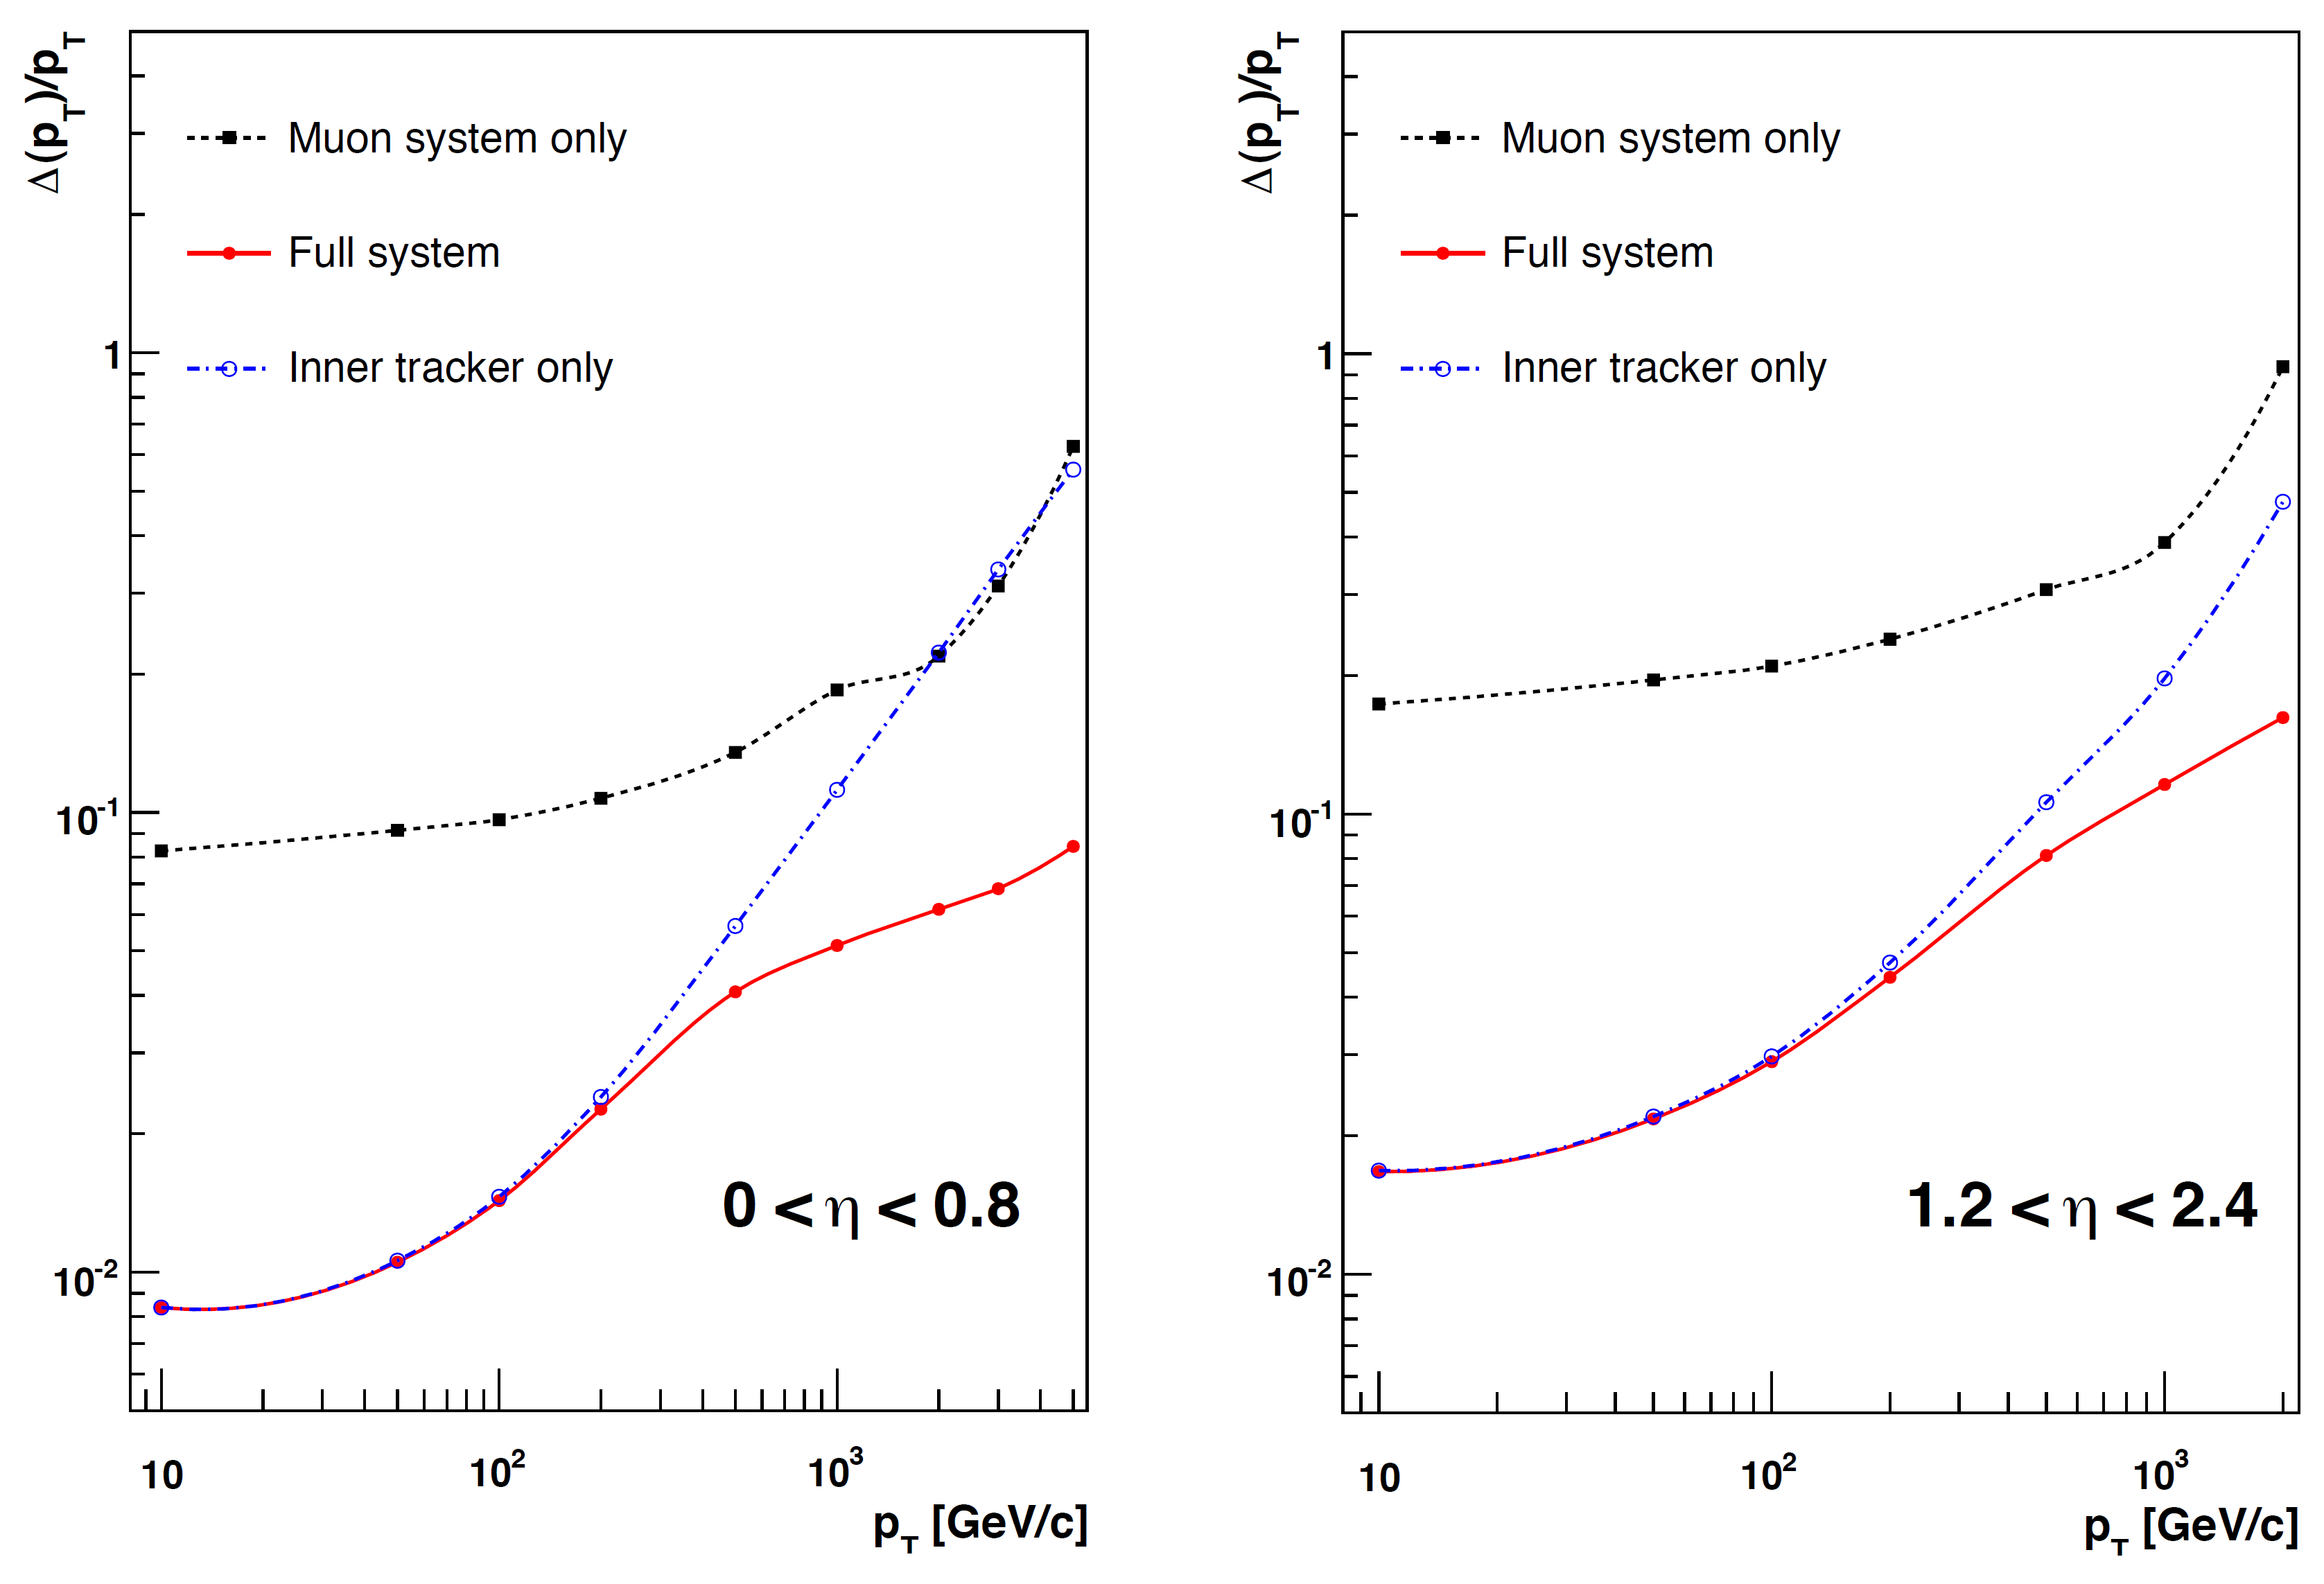
\includegraphics[width=0.6\textwidth]{images/muptres.png}
\caption{Muon \pt resolution as a function of the muon \pt in the barrel (left) and in the endcap (right) region. The resolution is provided for the measurement using the tracking system or the muon system only, as well as for the combination of the two methods.}\label{fig:muptres}
\end{figure}

Depending on the physics analysis, different muon definitions can be used by changing the selection on the muon identification variables, hence balancing between the muon identification efficiency and purity. The most widely used definition in physics analyses at CMS is the so-called \emph{Tight muon selection}\footnote{Small variations with respect to this baseline definition are adopted by the specific analyses.}. This selection requires the muon candidate to be reconstructed as a Global Muon and identified by the PF algorithm. The fit of the global track, which is required to include muon segments in at least two muon stations, must have a $\chi^2/d.o.f.$ less than 10 and use more than 10 inner tracker hits. The transverse impact parameter with respect to the primary vertex is required to be $|d_{xy}|<2$\,mm, significantly reducing the rate of muons from in flight decays, i.e. non-prompt muons. The requirements defining the Tight Muon identification are summarized in Table~\ref{tab:tightmuon}.

\begin{table}[htb]
\caption{Summary of the muon identification variables and the corresponding selections commonly used by physics analyses.}\label{tab:tightmuon}
\centering
\begin{tabular}{lc}
\toprule
Observable & Selection \\
\midrule
Is Global Muon & true \\
Is PF muon & true \\
Tracker layers with valid hits & $>5$ \\
Number of valid pixel hits & $>0$ \\
Number of valid muon hits & $>0$ \\
Number of matched muon stations & $>1$ \\
$\chi^2/d.o.f.$ & $<10$ \\
$d_{xy}(PV)$ & $< 0.2$\,cm \\
$d_{z}(PV)$ & $< 0.5$\,cm \\
\bottomrule
\end{tabular}
\end{table}

Another selection which is optimized for low-\pt muons coming from in flight decays is called \emph{Soft-Muon selection}. This selection requires the muon to be reconstructed as a Tracker Muon with additional loose cuts on the transverse and longitudinal impact parameters. This selection is commonly used to identify muons coming from B hadron decays.

\subsection{Muon isolation}
The isolation is one of the most powerful requirements to select prompt muons, as the ones produced by W or Z boson decays, and to reject muons produced by in flight decays. Indeed, prompt muons are expected to be isolated in the event, contrary to non-prompt muons that are generally produced within jets and characterized by many nearby particles.

Muons commonly used to reconstruct the W or Z boson decays are thus required to pass an isolation requirement, which includes a pile-up mitigation correction called ``$\Delta\beta$ correction''. This correction is needed to obtain a robust isolation definition that is less sensitive to the pile-up contribution. Indeed, simultaneous interactions manifest themselves as a mean energy deposited over all the detector acceptance that is not due to particles produced in the primary event, thus spoiling the isolation measurement. The relative isolation variable, usually called \emph{PF relative isolation}, is defined as follows:
\begin{equation}\label{eq:isomu}
I^{rel}_{\Delta\beta} = \left[  \sum_{ChH}\pt + max\left(0, \sum_{NH}\pt + \sum_{Ph}\pt - 0.5\sum_{ChHPU}\pt    \right)  \right]/\pt^\mathrm{muon} \quad .
\end{equation}

The sums in Eq.~\eqref{eq:isomu} are performed in a cone of radius $\Delta R < 0.4$ around the muon direction. The $ChH$ subscript refers to charged hadrons, $NH$ to neutral hadrons, $Ph$ to photons and $ChHPU$ to charged hadrons not arising from the primary vertex.

The cut applied on the isolation variable is analysis dependent, but a common value is $I^{rel}_{\Delta\beta} < 0.15$.

A different isolation definition is called \emph{Tracker relative isolation}, $I^{rel}_{trk}$, which is calculated as the scalar sum of all the \pt of the tracker tracks reconstructed inside a cone of radius $\Delta R < 0.3$ around the muon track direction.

\subsection{Muon momentum scale and resolution}
The measurement of the muon \pt is sensitive to the alignment of the tracker and muon chambers, material composition and distribution inside the detector and to the knowledge of the magnetic field produced by the solenoid. The imperfect knowledge of the magnetic field and the effect of the material distribution introduce a relative bias in the muon \pt that is generally independent on the \pt itself, while the effect of the alignment is known to produce a bias that increases linearly with the \pt.

Different methods are used to estimate the muon \pt scale and resolution effects and to determine the corresponding uncertainties depending on the \pt range. At low and intermediate \pt ($< 100$\,\GeV), the dimuon events arising from the $\mathrm{J/\Psi}$ and Z resonance decays are used to correct the \pt scale and to measure the \pt resolution. In the high \pt regime, the muon \pt scale and resolution are instead measured using cosmic ray muons. One of the methods that is commonly used in the intermediate \pt range is the \emph{MuScleFit} (Muon momentum Scale calibration Fit)~\cite{Chatrchyan:2012xi}, which provides the muon \pt scale corrections by fitting the Z boson mass peak in data and simulation. These corrections are meant to recover the bias of the Z mass peak with respect to the $\eta$ and $\phi$ coordinates of the muon. After applying these corrections, the relative \pt resolution ($\sigma(\pt)/\pt$) is measured as a function of $\eta$ and $\phi$ and is found to be on average of the order of 2\% in the barrel and up to 6\% in the endcaps, for muon \pt below 100\,\GeV.

\subsection{Electron reconstruction and identification}\label{sec:eleIdIso}

The electron reconstruction is based on the combination of tracker and ECAL information. The reconstruction technique starts by measuring the energy deposits in ECAL by electrons, which form a ``supercluster''. A supercluster is a group of one or more ECAL clusters associated using an algorithm that takes into account the characteristic shape of the energy deposited by electrons emitting \emph{bremsstrahlung} radiation in the tracker material. The supercluster shape is characterized by a narrow width profile in the $\eta$ coordinate spread over the $\phi$ direction. The superclusters are matched to tracks reconstructed in the tracker with the GSF algorithm in order to obtain an electron candidate. An additional reconstruction method, described in details in Refs.~\cite{CMS-PAS-EGM-10-004,Khachatryan:2015hwa}, is instead seeded by electron tracks reconstructed in the inner tracker layers.

Several strategies are used in CMS to identify prompt isolated electrons (characteristic of the signal processes of interest), and to separate them from background sources, mainly originating from photon conversions, jets misidentified as electrons, or electrons from semileptonic decays of b and c quarks. In order to achieve a good discrimination, several identification variables are used:
\begin{itemize}
\item $\Delta\eta_\mathrm{trk,SC}$ and $\Delta\phi_\mathrm{trk,SC}$: the variables measuring the spatial matching between the track and the supercluster in the $\eta$ and $\phi$ coordinates, respectively;
\item $\sigma_{i\eta,i\eta}$: a variable related to the calorimeter shower shape, measuring the width of the ECAL supercluster along the $\eta$ direction computed for all the crystals in the $5
\times 5$ block of crystals centred on the highest energy crystal of the seed supercluster;
\item $H/E$: the ratio between the energy deposited in the HCAL tower behind the ECAL seed and the supercluster seed energy;
\item $|1/E - 1/p|$: the difference of the inverse of energy $E$ measured in ECAL and the inverse of momentum $p$ measured in the tracker;
\item the number of missing hits in the back-propagation of the track to the interaction point;
\item $d_{xy}$ and $d_z$: the transverse and longitudinal impact parameters with respect to the primary vertex.
\item a photon conversion veto ($\gamma \to \mathrm{e^+ e^-}$) based on missing hits in the inner layers of the tracker.
\end{itemize}

Different working points are used, corresponding to different selections on the previously defined variables. One of the common working points used by several physics analyses, as the \hww analysis in this thesis, is the ``tight working point'', summarized in Table~\ref{tab:tightele}.

\begin{table}[htb]
\caption{Electron identification selections corresponding to the tight working point.}\label{tab:tightele}
\centering
\begin{tabular}{lcc}
\toprule
\multirow{2}{*}{Variable} & \multicolumn{2}{c}{Selection}\\
 & $|\eta_\mathrm{SC}|\leq 1.479$ & $1.479 < |\eta_\mathrm{SC}| \leq 2.5$ \\
\midrule
$\sigma_{i\eta,i\eta}$ & 0.01 & 0.028 \\
$|\Delta\eta_\mathrm{trk,SC}|$ & 0.009 & 0.007 \\
$|\Delta\phi_\mathrm{trk,SC}|$ & 0.03 & 0.09 \\
$H/E$ & 0.06 & 0.06 \\
$|1/E - 1/p|$ & 0.012 & 0.010 \\
$|d_{xy}|$ & 0.011\,cm & 0.035\,cm\\
$|d_{z}|$ & 0.047\,cm & 0.42\,cm\\
missing inner hits & $\leq 2$ & $\leq 1$\\
conversion veto & yes & yes \\
\bottomrule
\end{tabular}
\end{table}

\subsection{Electron isolation}
Selected electrons are required to pass an isolation requirement that includes a pile-up mitigation correction based on the electron effective catchment area, which is different in different $\eta$ ranges. The isolation variable is given by the following formula:
\begin{equation}
I^{rel}_{EA~corrected} = \left[ \sum_{ChH}\pt + max\left( 0, \sum_{Ph}\pt + \sum_{NH}\pt - \rho A \right) \right]/\pt^\mathrm{electron} \,
\end{equation}

\noindent where $ChH$ refers to charged hadrons, $Ph$ to photons, $NH$ to neutral hadrons, $\rho$ is the energy density due to pile-up events and $A$ is an effective area. The sums are performed inside a cone of radius $\Delta R < 0.4$ around the electron direction. The selection applied on this variable for the tight working point is $I^{rel}_{EA~corrected} < 0.04$.

\subsection{Electron momentum scale and resolution}
The electron momentum is estimated using a combination of the tracker and ECAL measurements. The ECAL energy response is calibrated before making the combination of the two measurements. Before doing the clustering, the energy response in individual crystals is calibrated and a correction factor is applied to take into account effects as energy leakage or changes in the crystal transparency induced by radiation~\footnote{The continuous monitoring of the crystals transparency is achieved by a laser-monitoring system.}. Then the supercluster energy is also corrected using an MVA technique, selecting $\mathrm{Z\to e^+ e^-}$ events in data and comparing to simulation. A detailed description of the techniques used to estimate the electron scale and resolution and the associated uncertainties is given in Ref.~\cite{Khachatryan:2015hwa}.



\subsection{Lepton identification and isolation efficiency}\label{sec:lepIdIsoEff}
The efficiency related to the identification and isolation selections applied to muons and electrons is generally estimated both in data and simulation, and simulated events are corrected for the observed differences by means of a scale factor ($SF$), defined as the ratio of the efficiency measured in data ($\varepsilon_\mathrm{data}$) and simulation ($\varepsilon_\mathrm{MC}$), i.e. $SF = \varepsilon_\mathrm{data}/\varepsilon_\mathrm{MC}$.

The identification and isolation efficiencies are measured using a Tag and Probe technique. 
The Tag and Probe technique is a method to estimate the efficiency of a selection on data. It can be applied whenever one has two objects in a given event by using one of the two, the \tg{}, to identify the process of interest and the second, the \probe{}, to actually measure the efficiency of the selection being studied.
Concerning the electron and muon case, the Tag and Probe method uses a known resonance (e.g. $\mathrm{J/\Psi}$, Z) to select particles of the desired type, and probe the efficiency of a particular selection criterion on these particles. In general the \tg{} is an object that passes a set of very tight selection criteria designed to isolate the required particle type. Tags are often referred to as a ``golden'' electrons or muons and the fake rate for passing tag selection criteria should be very small. A generic set of the desired particle type, the \probe{} (defined with potentially very loose selection criteria) is selected by pairing these objects with tags such that the invariant mass of the combination is consistent with the mass of the resonance. Combinatorial backgrounds may be eliminated through any of a variety of background subtraction methods such as fitting, or sideband subtraction. The definition of the probe objects depend on the specifics of the selection criterion being examined. The simple expression to get the efficiency $\varepsilon$ as a function of \pt and $\eta$ is given below:
\begin{equation}\label{eq:tagprobe}
\varepsilon(\pt,\eta) = \frac{ N^\mathrm{probe}_\mathrm{pass}}{N^\mathrm{probe}_\mathrm{pass} + N^\mathrm{probe}_\mathrm{fail}}
\end{equation}

For the estimation of the electron (muon) identification efficiency, the tag is chosen to be a well identified and isolated electron (muon), while the probe is chosen as an electron (muon) identified with loose selections. The invariant mass of the \tp pair is required to be within a window around the Z boson mass (the effect of changing the Z mass window is included as a systematic uncertainty). After that, the probe is required to pass the identification selections discussed before for electrons and muons, and the efficiency is computed both in data and simulation. A scale factor is then calculated by taking the ratio of the two efficiencies and applied to reweight simulated events.

There are two methods to measure the efficiencies: the counting method consists in simply computing the ratio of probe events that pass the selections and total number of probe events, as shown in Eq.~\eqref{eq:tagprobe}. This method can be used when the tag requirement selects a very pure set of events, with a small background contribution. The other approach is the fitting method, which is used when the background contamination is not negligible. In this latter case, which represents the commonly used method for estimating the lepton identification and isolation efficiencies, the invariant mass distribution of the tag-probe pair for signal and background is fitted choosing proper functions. The signal plus background fit is performed simultaneously in two categories, corresponding to events in which the probe lepton passes or fails the identification requirements, and separately in bins of $\eta$ and \pt.

A similar approach is used to estimate the lepton isolation efficiency, requiring the probe lepton to pass the isolation requirements instead of the identification ones and calculating the corresponding scale factor.

The electron identification and isolation efficiency and the scale factor for the requirements described in Sec.~\ref{sec:eleIdIso} are shown in Fig.~\ref{fig:eleIdIso}.

\begin{figure}[htb]
\centering
%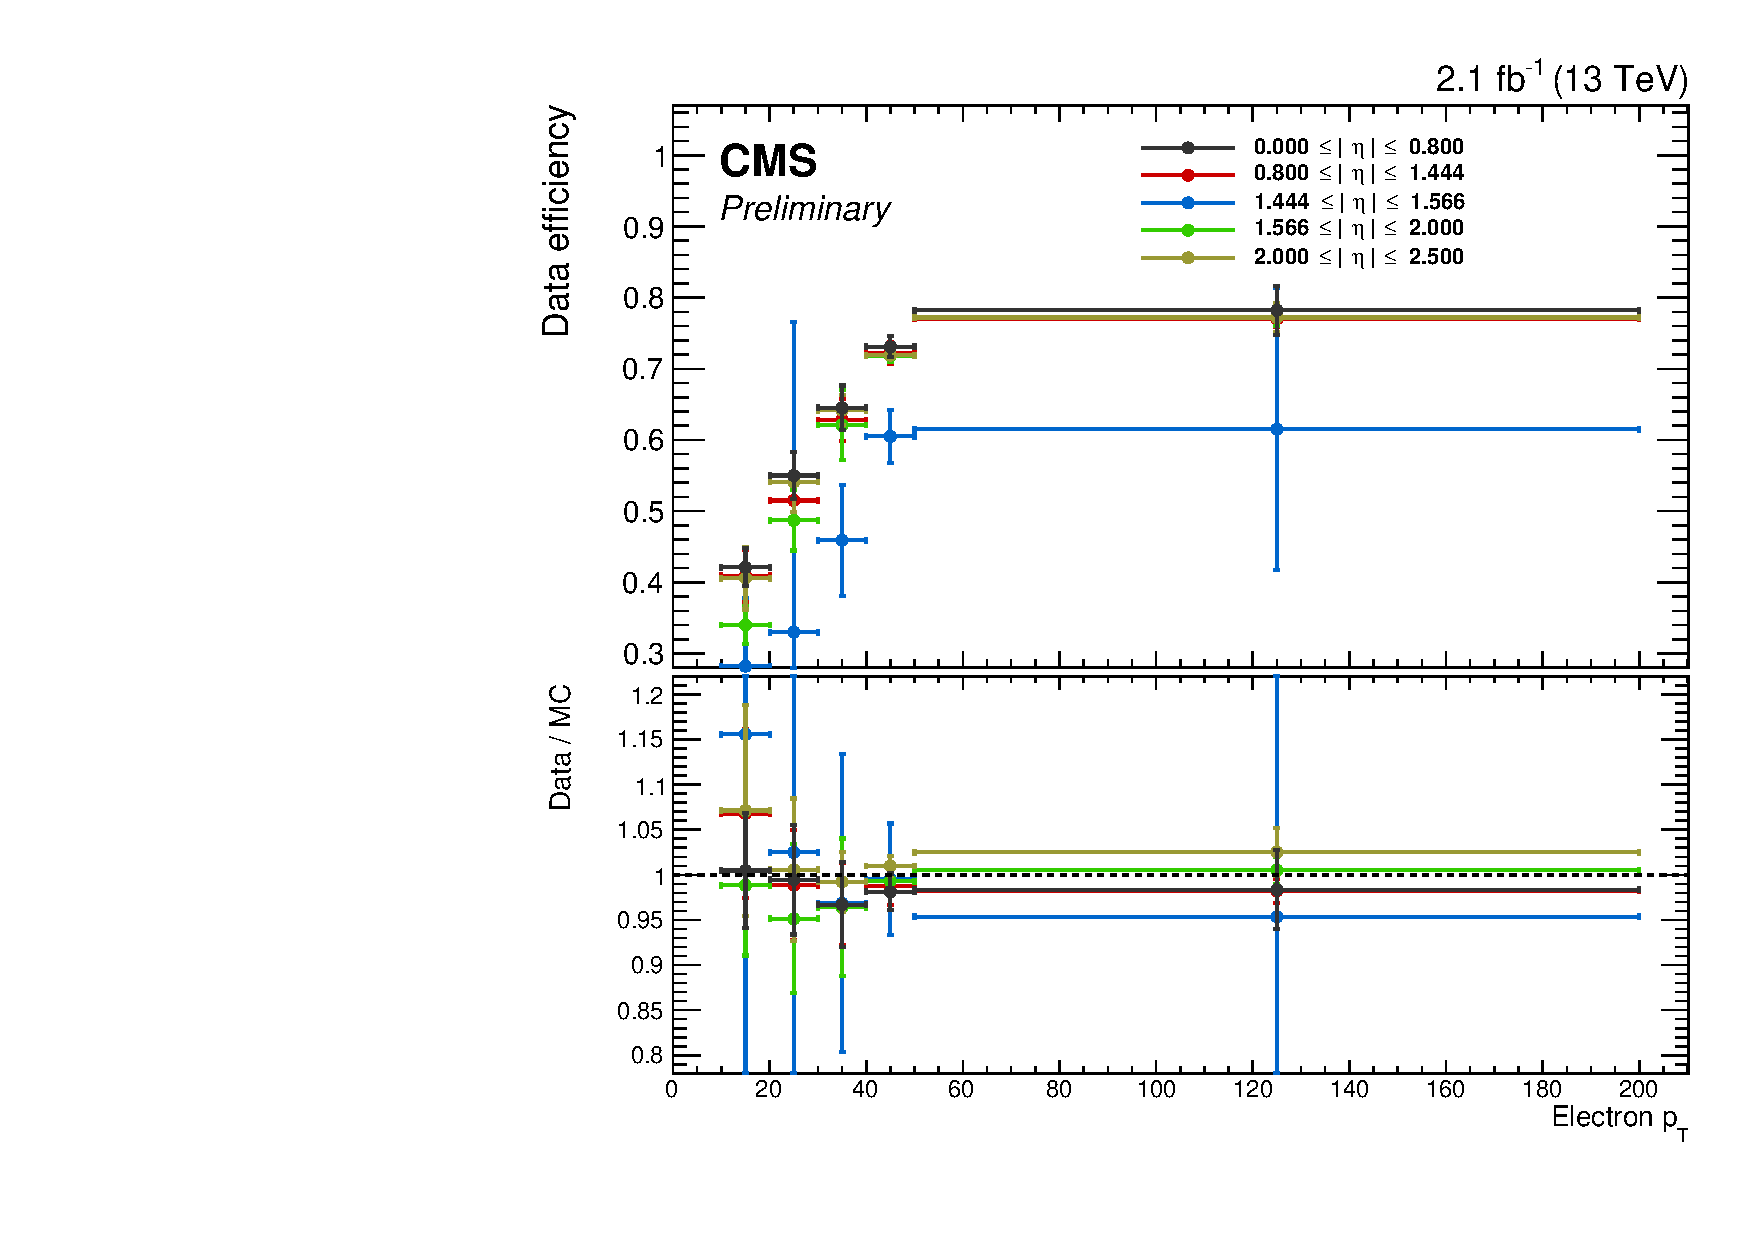
\includegraphics[width=0.5\textwidth]{images/effEleIdIso.pdf}
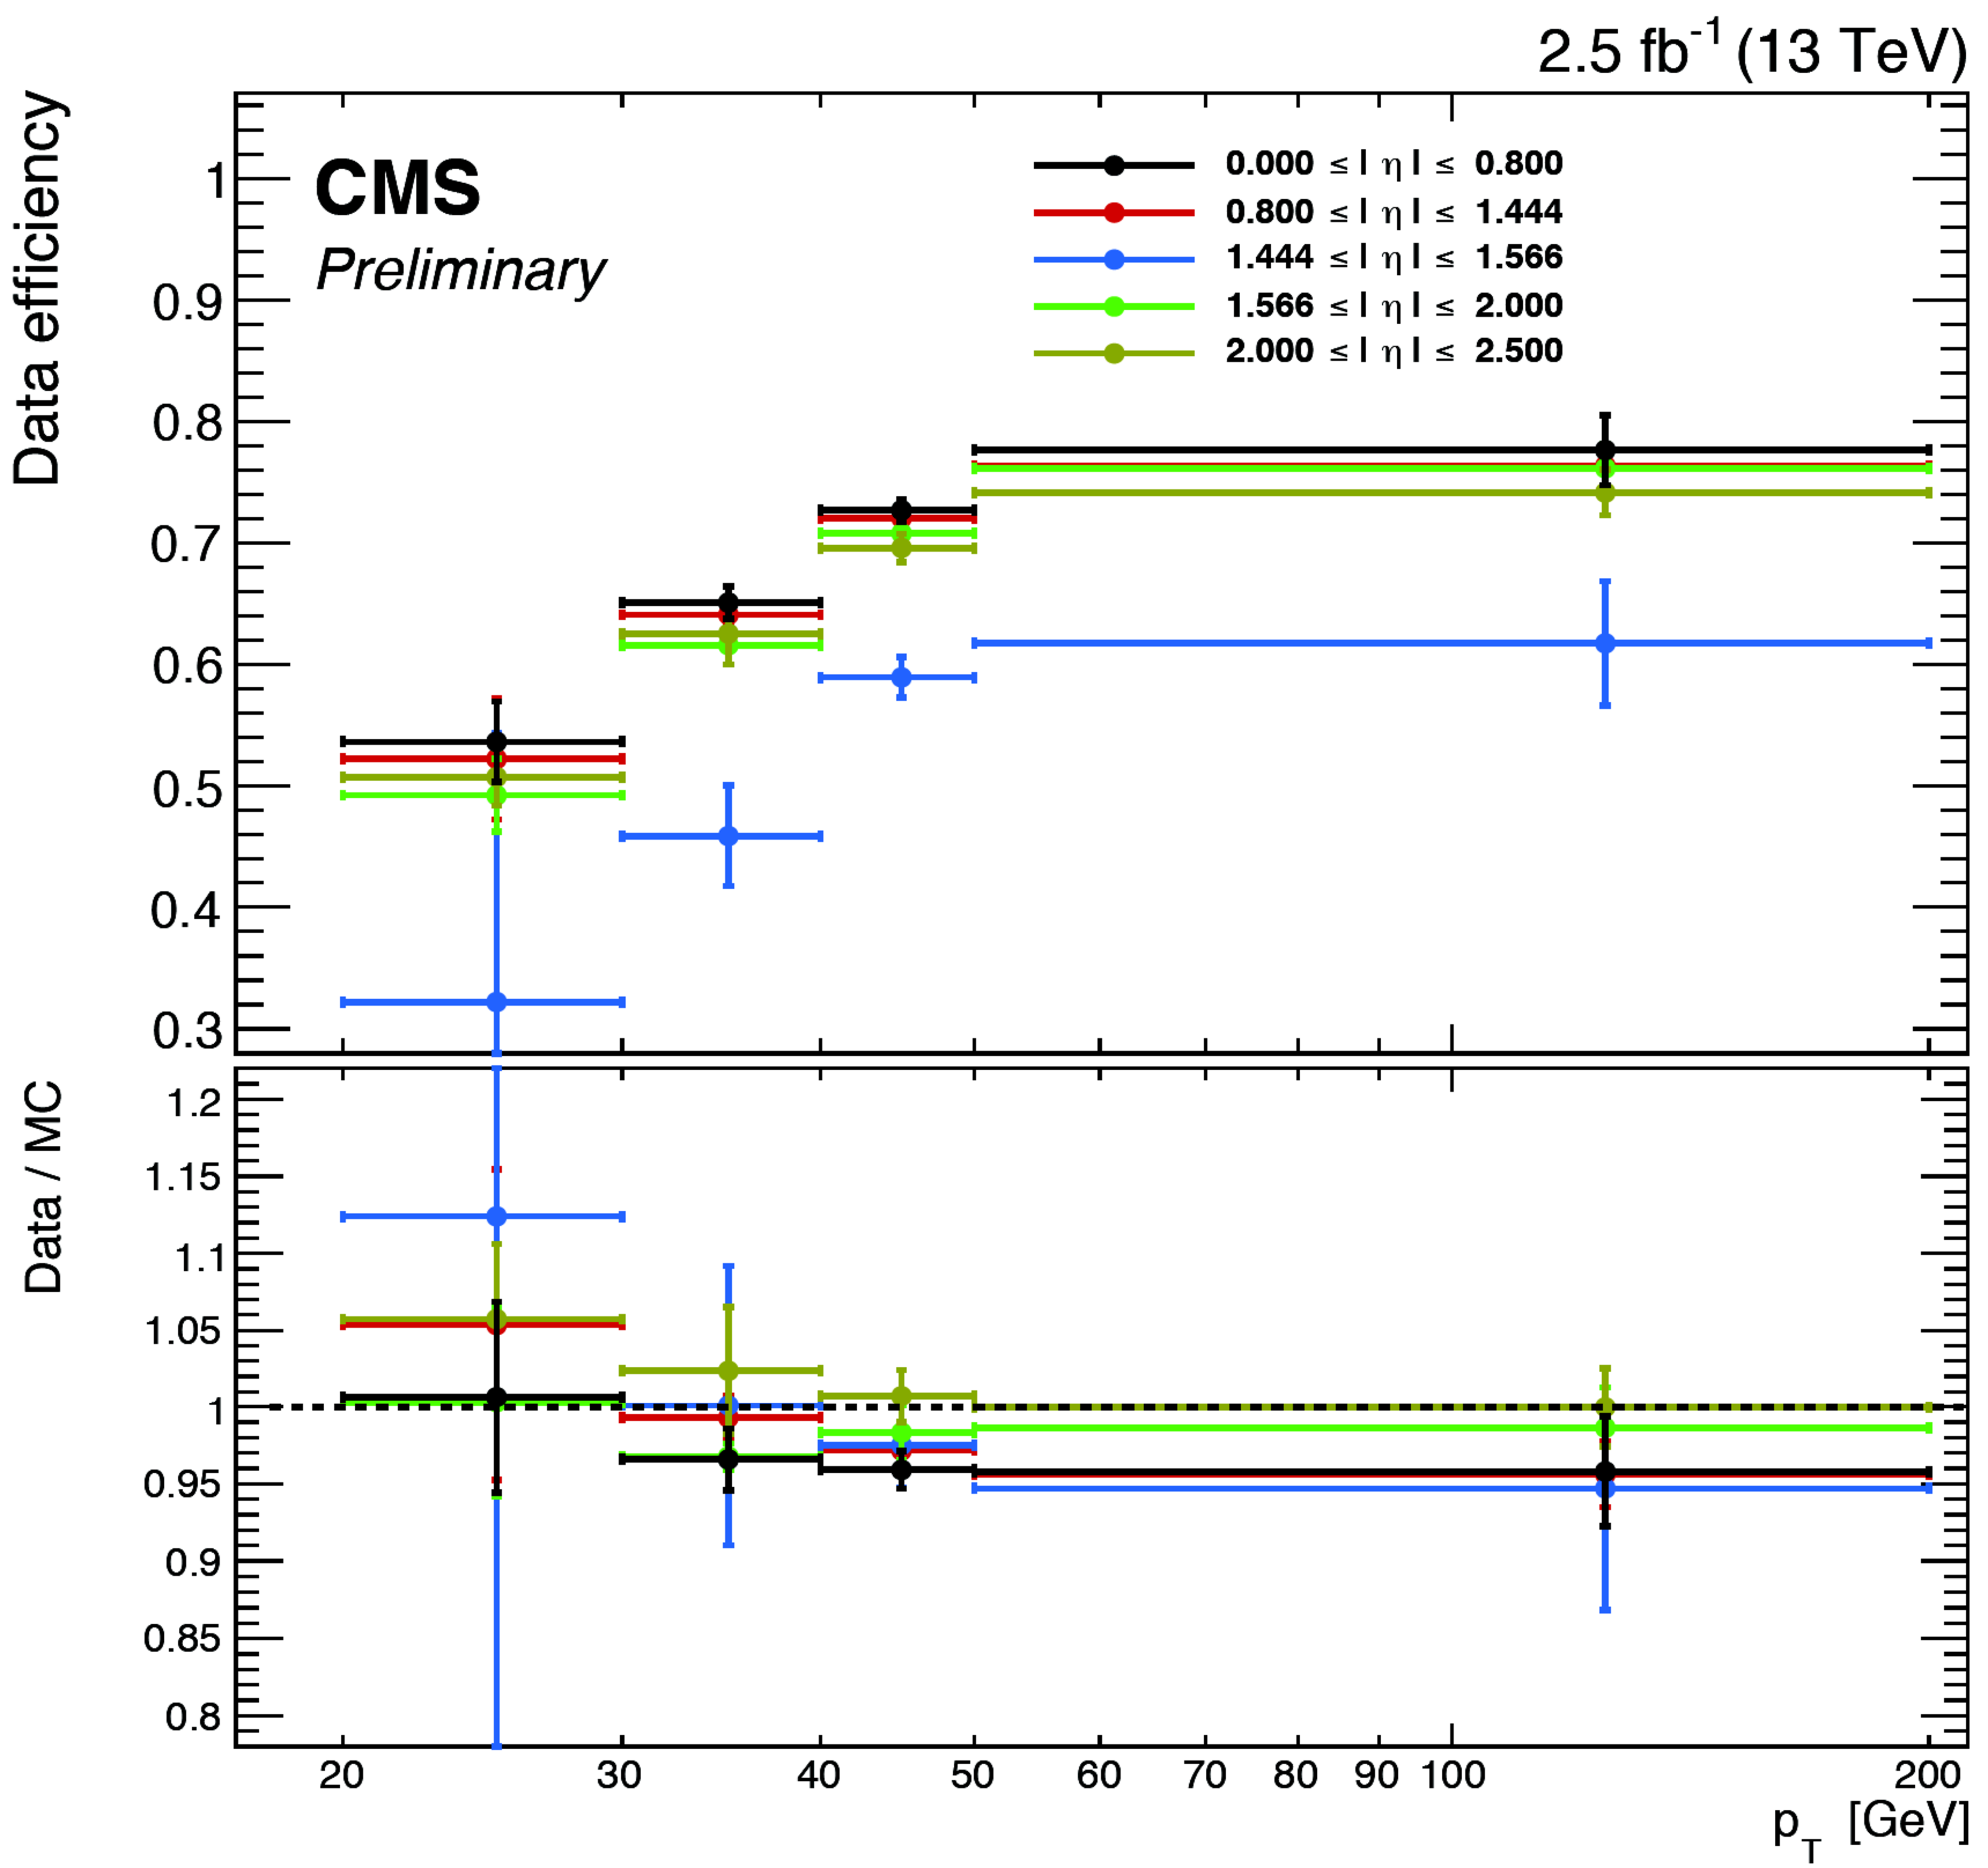
\includegraphics[width=0.45\textwidth]{images/eleIdIsoEff.pdf}
\caption{Electron identification and isolation efficiencies in data (top panel) and data/simulation scale factor (bottom panel), as a function of the electron \pt and for different $\eta$ bins.}\label{fig:eleIdIso}
\end{figure}
	
The identification and isolation efficiency and the scale factor for muons, according to the requirements in Table~\ref{tab:tightmuon}, are shown in Fig.~\ref{fig:muIdIso}.
	
\begin{figure}[htb]
\centering
\subfigure[]{
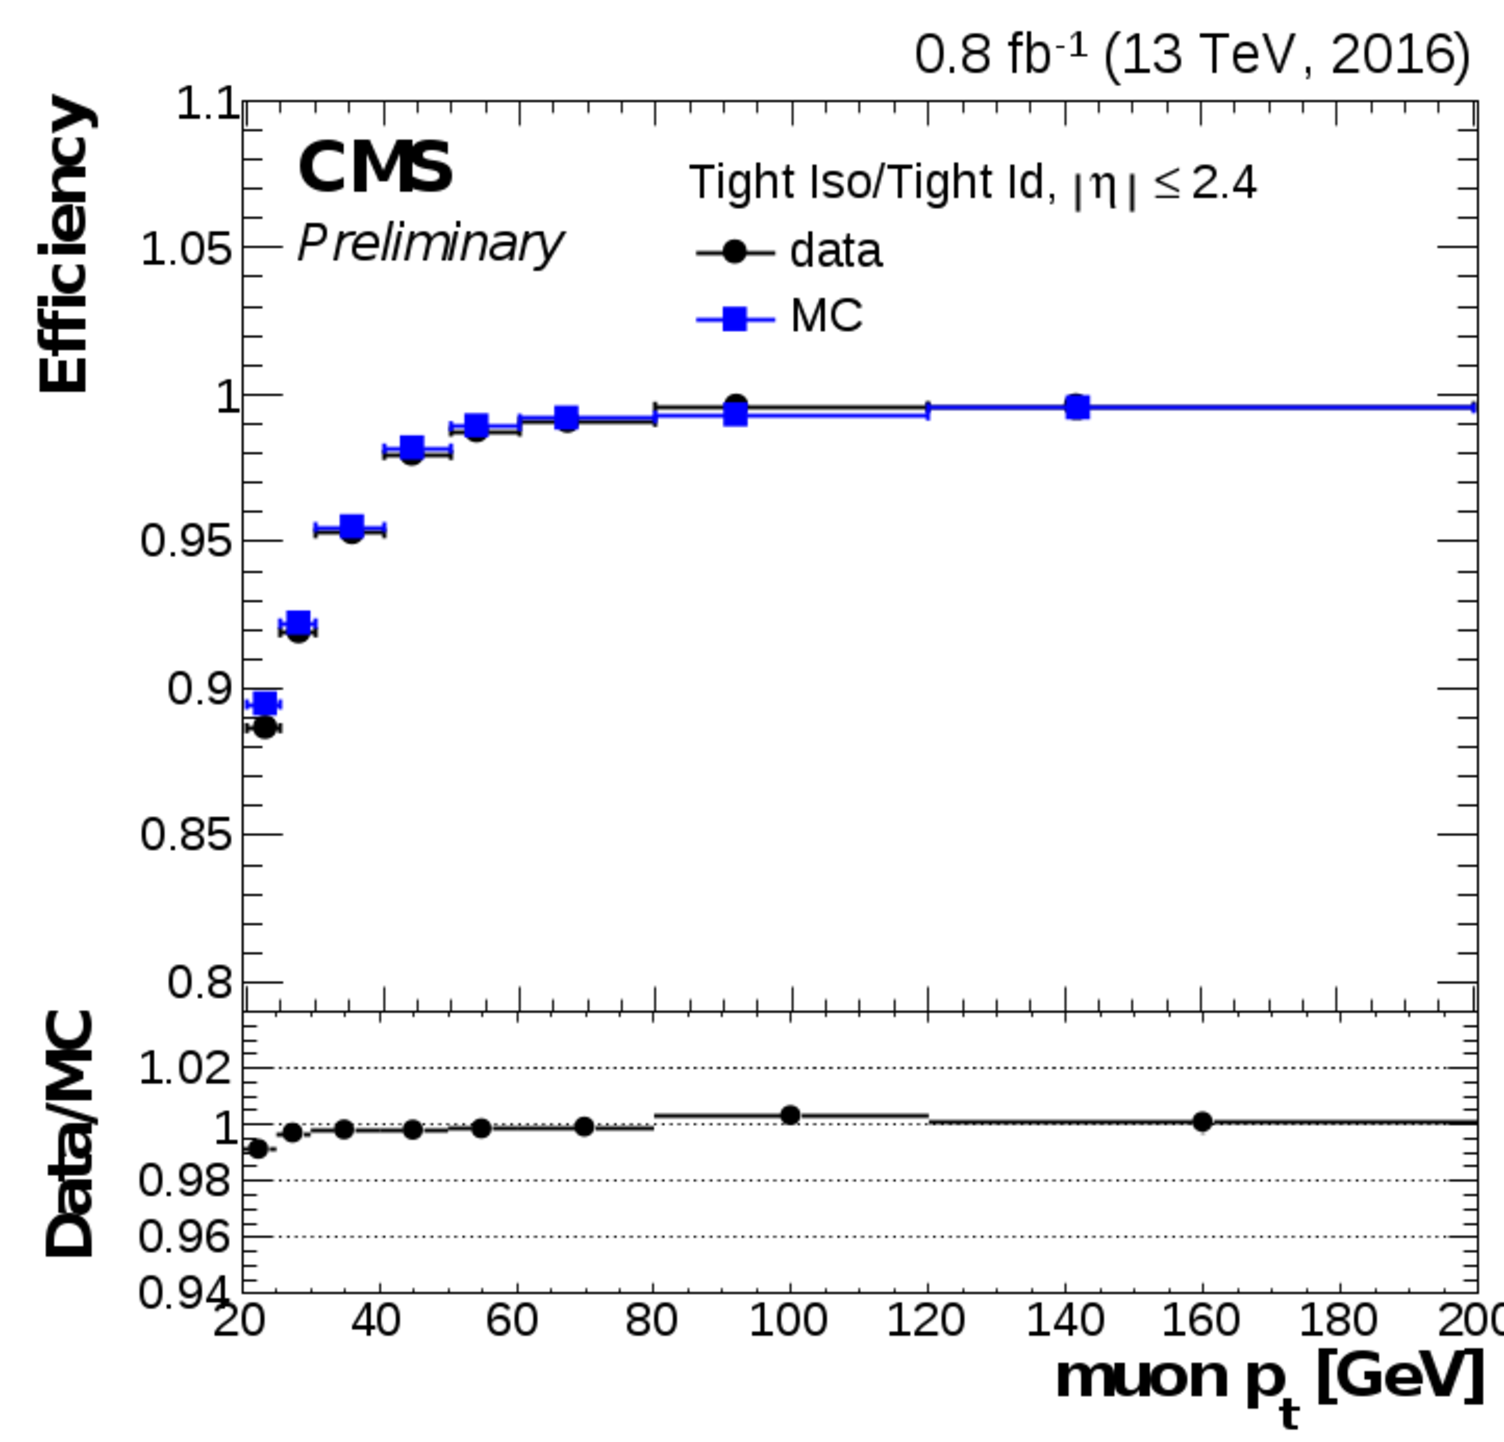
\includegraphics[width=0.45\textwidth]{images/muIdIsoEffPt.pdf}
}
\subfigure[]{
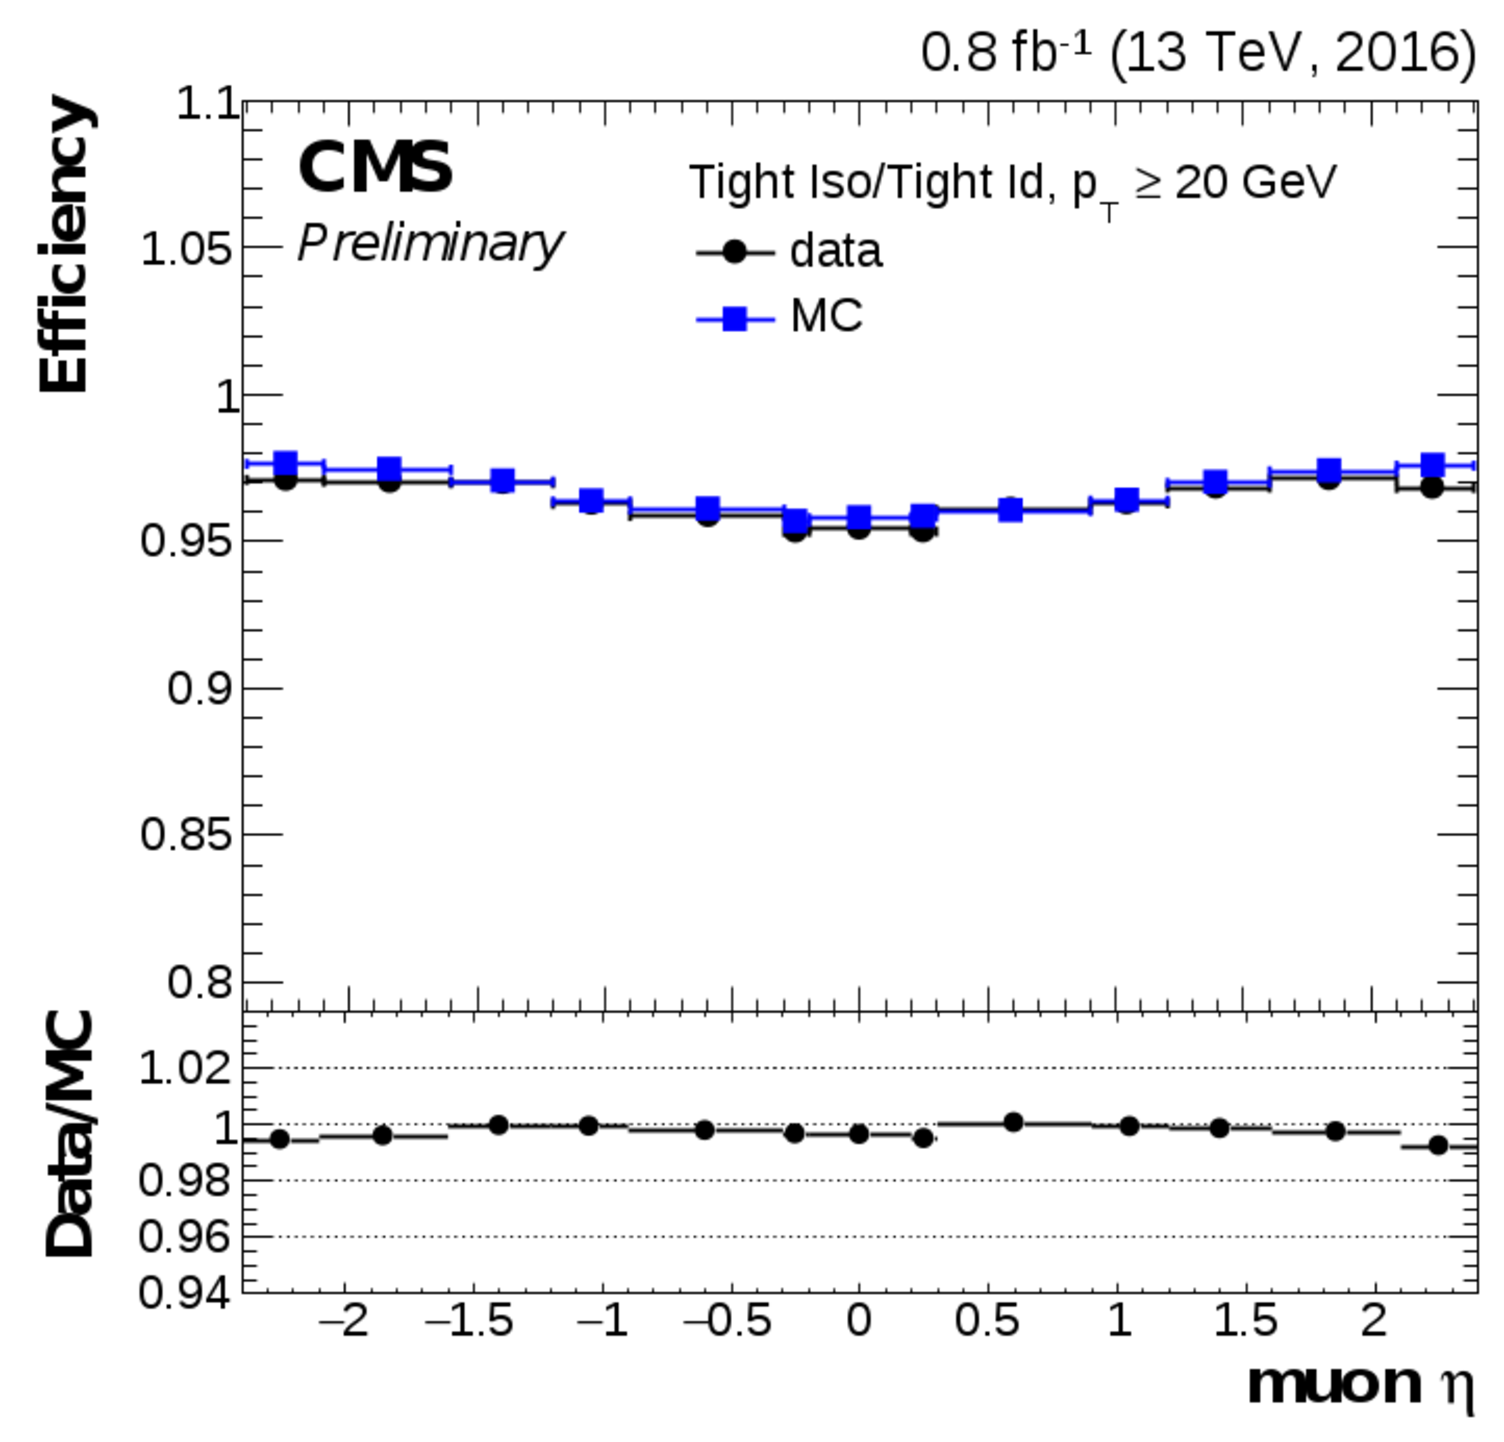
\includegraphics[width=0.45\textwidth]{images/muIdIsoEffEta.pdf}
}
\caption{Muon identification and isolation efficiencies in data and simulation (top panels) and data/simulation scale factor (bottom panels), as a function of the muon \pt (a) and $\eta$ (b).}\label{fig:muIdIso}
\end{figure}	
	
	
\subsection{Lepton trigger efficiency}\label{sec:trigeff}
Analyses that involve leptons in the final state generally select the interesting events using lepton triggers. For instance, the \hwwllnn channel is characterized by the presence of two leptons in the final state, thereby both single lepton and double lepton triggers are used. The lepton triggers at the HLT level are characterized by \pt thresholds above which the trigger efficiency is very high (plateau region). Nevertheless, the trigger efficiency as a function of the lepton \pt is not a step function, but is characterized by a steep increase of the efficiency around the \pt threshold (turn-on region). The simulated samples thus need to be corrected in order to properly take into account the trigger efficiency. This can be achieved in two ways: including the HLT trigger in the event simulation or calculating the trigger efficiency in data and then applying it on simulated events. Several analyses, such as those related to the \hwwllnn channel, opt for the second approach.

The trigger efficiency for single and double lepton triggers is calculated in bins of $\eta$ and \pt using a Tag and Probe technique similar to the one described in Sec.~\ref{sec:lepIdIsoEff}, separately for muons and electrons. Since the triggered events arise from a mixture of two different triggers, the combined efficiency has to be computed and applied to simulated samples as an event weight. In the following, the approach used in the \hwwllnn analyses is described.

The event efficiency $\varepsilon_\mathrm{ev}$ for an event with two leptons to pass the single lepton trigger is given by the following formula:
\begin{equation}\label{eq:single_trigg}
\varepsilon_\mathrm{ev} = 1 - (1-\varepsilon_{S,\ell1})\cdot(1-\varepsilon_{S,\ell2})\quad,
\end{equation}

\noindent where $\varepsilon_{S,\ell1}$ and $\varepsilon_{S,\ell2}$ are the efficiencies for the leading and subleading lepton to pass the single lepton trigger. In other words, the dilepton event passes the single lepton trigger if either one of the two leptons passes the single lepton trigger, unless both fail to pass it. 

For double lepton triggers the efficiency is calculated separately for each leg of the trigger. In the calculation of the efficiencies the two trigger legs are considered independent, given that the correlations are very small. The combined efficiency is then used as a kinematics-dependent weight to be applied on simulated events. The event efficiency can be written as:
\begin{equation}\label{eq:double_trigg}
\varepsilon_\mathrm{ev}  = \varepsilon_{D,\ell1}^\mathrm{lead} \cdot \varepsilon_{D,\ell2}^\mathrm{trail} + (  1 -  \varepsilon_{D,\ell1}^\mathrm{lead} \cdot \varepsilon_{D,\ell2}^\mathrm{trail})\cdot\varepsilon_{D,\ell1}^\mathrm{trail} \cdot \varepsilon_{D,\ell2}^\mathrm{lead} \quad,
\end{equation}

\noindent where $\varepsilon_{D,\ell1}^{\mathrm{lead}(trail)}$ is the efficiency of the first lepton to pass the leading (trailing) leg of the double lepton trigger, and $\varepsilon_{D,\ell2}^{\mathrm{lead}(trail)}$ is the efficiency of the second lepton to pass the leading (trailing) leg of the double lepton trigger. The final event efficiency applied to reweight the events in simulation is given by the boolean OR of the event efficiencies corresponding to the single and double lepton triggers, which using Eqs.~\eqref{eq:single_trigg} and ~\eqref{eq:double_trigg}, can be written as:
\begin{equation}
\begin{split}
\varepsilon_\mathrm{ev} & = 1 - (1-\varepsilon_{S,\ell1})\cdot(1-\varepsilon_{S,\ell2}) + \\
                     & + (1-\varepsilon_{S,\ell1})\cdot(1-\varepsilon_{S,\ell2}) \cdot \\
                     & \cdot [ \varepsilon_{D,\ell1}^\mathrm{lead} \cdot \varepsilon_{D,\ell2}^\mathrm{trail} + (  1 -  \varepsilon_{D,\ell1}^\mathrm{lead} \cdot \varepsilon_{D,\ell2}^\mathrm{trail})\cdot\varepsilon_{D,\ell1}^\mathrm{trail} \cdot \varepsilon_{D,\ell2}^\mathrm{lead} ] \quad.
\end{split}
\end{equation}

%The term that multiplies the double lepton trigger event efficiency is needed to ensure that the events passing the double lepton trigger do not pass also the single lepton trigger.




\section{Jets reconstruction and identification}\label{sec:jets}

Jets are the experimental signature of quarks and gluons produced in high energy physics processes. They arise from the hadronization of partons, which forms collimated sprays of particles, and play a predominant role in hadron colliders like the LHC, where the production cross section is very large. In this section, the jet reconstruction techniques used in CMS are described.

\subsection{Jet reconstruction in CMS}

The majority of physics analyses involving jets in the final state make use of particle flow jets. The PF jets are reconstructed using the technique described in Sec.~\ref{sec:PF}, clustering all particles reconstructed with the PF algorithm, without any distinction of type and energy threshold. This method allows a remarkable improvement in the jet momentum and spatial resolutions with respect to the calorimeter jets, which are instead reconstructed using solely the information from the calorimeters, as the use of the tracker information provides a better \pt resolution for the charged particles constituting the jets\footnote{On average, the typical jet energy fractions carried by charged particles, photons and neutral particles are 65\%, 25\% and 10\%, respectively.}. 

Jets are defined through sequential, iterative clustering algorithms that combine the four-momenta of input particles until certain conditions are satisfied and jets are formed~\cite{Salam:2009jx}. Several algorithms are available for jet clustering, characterized by different features. From a theoretical point of view, an ideal jet clustering algorithm should fulfil the following requirements~\cite{Blazey:2000qt}:
\begin{itemize}
\item \emph{Infrared safety}: infrared singularities should not appear in the perturbative calculations and the solutions of the algorithm should be insensitive to soft radiation in the event;
\item \emph{Collinear safety}: collinear singularities should not appear in the perturbative calculations and jets should be insensitive to collinear radiation in the event;
\item \emph{Invariance under boosts}: the solutions of the algorithm should be the same independently of boosts in the longitudinal direction. This is particularly important for pp colliders, where the centre-of-mass of the individual proton proton collisions is typically boosted along the beam direction;
\item \emph{Order independence}: the algorithm should find the same jets at parton, particle and detector level;
\item \emph{Straightforward implementation}: the algorithm should be straightforward to implement in perturbative calculations.
\end{itemize}
The ideal algorithm should also follow some experimental attributes. Among them, the performance of the algorithm should be as independent as possible of the detector that provides the data, the algorithm should not amplify the inevitable effects of resolution smearing and angle bias and should not be strongly affected by pile up and high beam luminosities. Furthermore, the algorithm should be easy to implement, efficient to identify all possible jet candidates and should keep at an acceptable level the necessary computing resources.

Two main classes of jet clustering algorithms can be defined. The first one consists in the ``cone'' recombination, where jets are reconstructed associating together particles whose trajectories lie within a cone of radius $\Delta R$ in the $\eta$--$\phi$ plane. The second class of algorithms uses the sequential recombination scheme, that iteratively recombine the closest pair of particles according to some distance measure. The standard algorithms used by CMS are the SISCone, which is a ``cone'' recombination algorithm, and the $k_t$, anti-$k_t$ and \emph{Cambridge Aachen} (CA) algorithms, which instead belong to the sequential recombination class.
All the analyses presented in Secs.~\ref{chap4}, \ref{chap5} and \ref{chap6} make use of the sequential recombination scheme, in particular of the anti-$k_t$ algorithm with $R=0.4$, which is briefly described in the following.

The $k_t$, anti-$k_t$ and CA algorithms are infrared and collinear safe algorithms characterized by the introduction of two definitions of distance: $d_{ij}$, the distance the two objects $i$ and $j$, and $d_{iB}$, the distance between the object $i$ and the beam. These distances are defined by the following equations:
\begin{equation}\label{eq:jetalgo}
\begin{split}
d_{ij} &= min\left(k_{ti}^{2p}, k_{tj}^{2p} \right) \frac{\Delta_{ij}^2}{R^2} \quad,\\
d_{iB} &= k_{ti}^{2p} \quad,
\end{split}
\end{equation}
where $\Delta_{ij} = (y_i - y_j)^2 + (\phi_i - \phi_j)^2$ and $k_ti$, $y_i$ and $\phi_i$ are the transverse momentum, rapidity and azimuthal angle of the particle $i$, respectively. In these formulas, $R$ represents the radial parameter and $p$ is a parameter that is 1 for $k_t$, 0 for CA and $-1$ for anti-$k_t$ algorithm. The algorithm proceeds as follows:
\begin{itemize}
\item the distances $d_{ij}$ are calculated for all pair of particle $i,j$ and the distances $d_{iB}$ are calculated for each particle $i$, according to Eq.~\eqref{eq:jetalgo};
\item the smallest distance, which could be either of type $d_{ij}$ or $d_{iB}$, is identified;
\item if the smallest distance is a $d_{ij}$, the particles $i$ and $j$ are combined into a single new particle summing their four-momenta and the algorithm restarts from the first step;
\item otherwise, if it is a $d_{iB}$, $i$ is declared to be a final state jet and the algorithm returns to the first step;
\item the procedure is repeated until no particles are left.
\end{itemize}

The physical difference between the three algorithms is the momentum weighting. For the $k_t$ algorithm, the weighting proportional to $k_t^2$ implies that jets are reconstructed starting from particles with low transverse momentum. Moreover this algorithm produces jets with irregular borders, thereby complicating the correction for effects such as pile up. For the CA algorithm there is no transverse momentum weighting, and the particles are merged following just an angular approach, based on the distance $\Delta_{ij}$. Also this algorithm leads to jets with irregular borders. Finally, the anti-$k_t$ algorithm, uses a weighting proportional to $1/k_t^2$, favouring the merging of high transverse momentum particles. In this case the jets grow around the particles with highest transverse momenta and the jets have a circular shape. 

Jets reconstructed with different algorithms starting from the same set of simulated particles are shown in Fig.~\ref{fig:jets}.

\begin{figure}[htb]
\centering
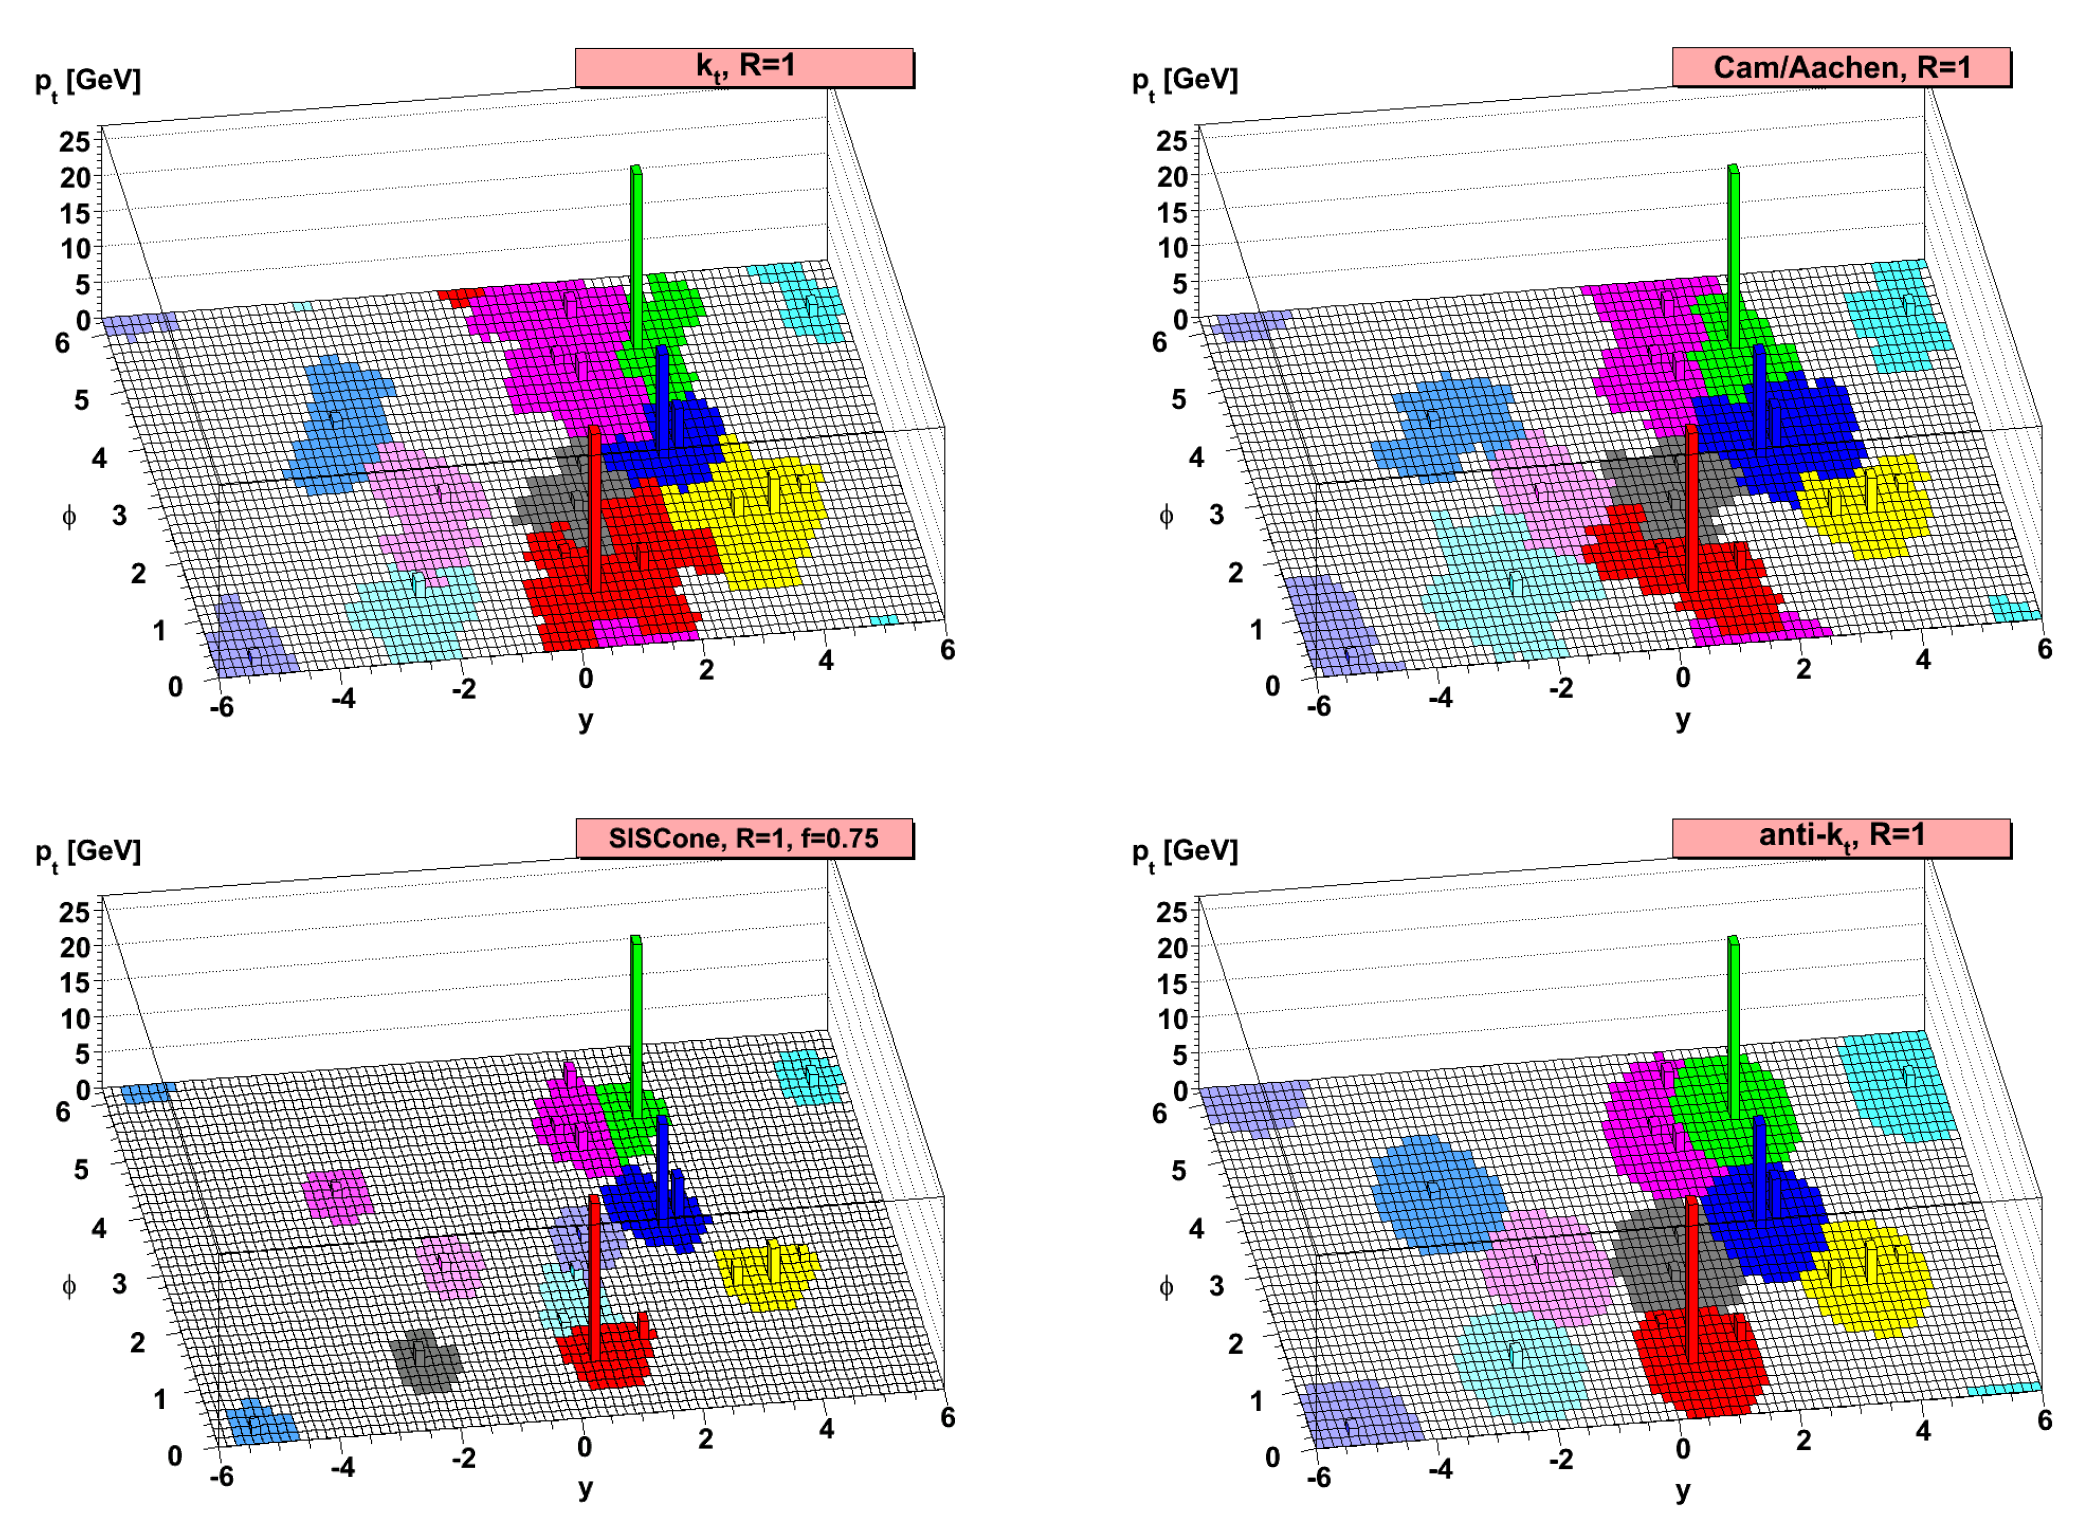
\includegraphics[width=0.7\textwidth]{images/jets.png}
\caption{Jets reconstructed with different algorithms starting from the same set of simulated particles. The jets reconstructed with the sequential recombination algorithms described in the text are shown, as well as with the SISCone algorithm.}\label{fig:jets}
\end{figure}

\subsection{Jet energy correction}

The purpose of jet energy correction is to relate, on average, the jet energy measured in the detector to the true energy of the corresponding final state particle or parton jet. The latter is obtained in simulation by clustering, with the same algorithm used for jets in the detector, all the stable particles, i.e. with $c\tau > 1$\,cm, produced in the event excluding neutrinos. This mismatch is mainly ascribable to the non uniform and linear response of the CMS calorimeters, to the electronics noise and to pile up. For this reason, CMS has developed a sequential procedure to calculate and apply the \emph{jet energy corrections} (JEC)~\cite{Chatrchyan:2011ds}.

The correction is applied as a multiplicative factor $\mathcal{C}$ to each component of the raw jet four-momentum $p_\mu^\mathrm{raw}$ (components are indexed by $\mu$ in the following):
\begin{equation}
p_\mu^\mathrm{cor} = \mathcal{C}\cdot p_\mu^\mathrm{raw} \quad,
\end{equation}
where $p_\mu^\mathrm{cor}$ is the corrected jet four-momentum. The correction factor is composed of the offset correction $C_\mathrm{offset}$, the MC calibration factor $C_\mathrm{MC}$, and the residual calibrations $C_\mathrm{rel}$ and $C_\mathrm{abs}$ for the relative and absolute energy scales, respectively. The offset correction removes the extra energy due to noise and pile up, and the MC correction removes the bulk of the non-uniformity in $\eta$ and the non-linearity in \pt. Finally, the residual corrections account for the small differences between data and simulation. The various components are applied in sequence as described by the equation below:
\begin{equation}
\mathcal{C} = C_\mathrm{offset}(\pt^\mathrm{raw}) \cdot C_\mathrm{MC}(\pt',\eta) \cdot C_\mathrm{rel}(\eta) \cdot C_\mathrm{abs}(\pt'') \quad ,
\end{equation}
where $\pt'$ is the jet \pt after applying the offset correction and $\pt''$ is the jet \pt after applying all previous corrections. Each component is briefly described in the following sections.

\subsubsection{Offset correction}
 
The offset correction purpose is to estimate and subtract, on average, the energy contribution that is not associated with the hard scattering in the event. The energy excess includes contributions from electronics noise and pile up. The approach followed for the estimation of the offset correction is known as \emph{Jet Area Method}. For each event, an average \pt-density per unit area, $\rho$, is estimated, characterizing the soft jet activity. This \pt-density represents the combination of the underlying event, the electronics noise and the pile up effects. 
The two latter components contaminate the hard jet energy measurement and need to be
corrected for with the offset correction. The key element for this approach is the jet area $A_j$.
A very large number of infinitely soft four-momentum vectors (soft enough not to change the properties of the true jets) are artificially added in the event and clustered by the jet algorithm together with the true jet components. The extent of the region in the $\eta$--$\phi$ space occupied by the soft particles clustered in each jet defines the active jet area. The \pt-density $\rho$ is calculated with the $k_t$ algorithm with a distance parameter $R=0.6$. The quantity $\rho$ is estimated event by event as the median of the distribution of the variable $p_{\mathrm{T}j}/A_j$, where $j$ runs over all jets in the event, and is not sensitive to the presence of hard jets in the event. At the detector level, the measured density $\rho$ is the convolution of the true particle-level activity (underlying event, pile-up) with the detector response to the various particle types. The event-by-event and jet-by-jet offset correction can thus be defined as:

\begin{equation}
C_\mathrm{offset}(\pt^\mathrm{raw},A_j,\rho) = 1 - \frac{\left( \rho - \langle\rho_\mathrm{UE}\rangle \right)\cdot A_j}{\pt^\mathrm{raw}}\quad .
\end{equation}

In the formula above, $\langle\rho_\mathrm{UE}\rangle$ represents the average \pt-density component due to the underlying event and electronics noise, and is measured in events with exactly one reconstructed primary vertex, i.e. no pile up.

An additional pile up subtraction method that is used in CMS is called \emph{Charged Hadron Subtraction}. This method makes use of PF jets and exploits the excellent CMS tracking capabilities to identify and remove charged hadrons inside jets, which are known to originate from pile up vertices. This is a particle-by-particle method that is applied to jets before calculating the offset correction.

\subsubsection{MC calibration correction}

The MC calibration is based on the simulation and corrects the energy of the reconstructed jets such that it is equal on average to the energy of the generated jets. In order to evaluate this correction, simulated QCD events are generated and then processed through the CMS detector simulation, based on the \textsc{Geant4} software. The jet reconstruction in simulation is identical to the one applied to the data. Each reconstructed jet is spatially matched, in the $\eta$--$\phi$ space, to a generated jet by requiring $\Delta R < 0.25$. In each bin of the generated jet transverse momentum $\pt^\mathrm{gen}$, the response variable $\mathcal{R}=\pt^\mathrm{reco}/\pt^\mathrm{gen}$ and the reconstructed jet transverse momentum $\pt^\mathrm{reco}$, are saved. The average correction in each bin is therefore defined as:

\begin{equation}
C_\mathrm{MC}(\pt^\mathrm{reco}) = \frac{1}{\langle R \rangle} \quad,
\end{equation}

and is expressed as a function of the average reconstructed jet \pt, $\langle \pt^\mathrm{reco} \rangle$.

\subsubsection{Relative jet energy scale}

The goal of the relative jet energy scale correction is to make the jet response flat versus $\eta$. This is achieved by employing a Tag and Probe technique, selecting di-jet events in data. The size of this residual correction is of the order of 2--3\% in the central $\eta$ region, while it goes up to about 10\% in the forward region.

\subsubsection{Absolute jet energy scale}

The goal of the absolute jet energy scale correction is to make the jet response at versus \pt. The absolute jet energy response is measured in the reference region $|\eta|<1.3$ with the \emph{Missing Transverse Energy Projection Fraction} (MPF) method~\cite{Abbott:1998xw}, using $\gamma+\mathrm{jets}$ and Z$+\mathrm{jets}$ events. The method is used to estimate the absolute jet energy correction and is based on the fact that $\gamma+\mathrm{jets}$ and Z$+\mathrm{jets}$ events have no intrinsic \MET and that, at parton level, the $\gamma$ and Z boson are perfectly balanced by the hadronic recoil in the transverse plane.

\subsubsection{Jet energy uncertainties}

The uncertainties in the jet energy estimation arise from several different sources. Generally these can be categorized as follows:
\begin{itemize}
\item physics modelling in MC such as showering, underlying event, etc.;
\item MC modelling of true detector response and properties;
\item potential biases in the methodologies used to estimate the corrections.
\end{itemize}
The sources are combined in different groups: absolute scale, relative scale, pile up, jet flavor and time stability. In Fig.~\ref{fig:JECunc} the effect of each group of uncertainties is shown together with the total uncertainty obtained summing all sources in quadrature, both as a function of $\eta$ and \pt. The pile up uncertainty dominates for low values of the jet \pt while the relative and absolute uncertainties are more important in the high \pt region.

\begin{figure}[htb]
\centering
\subfigure{
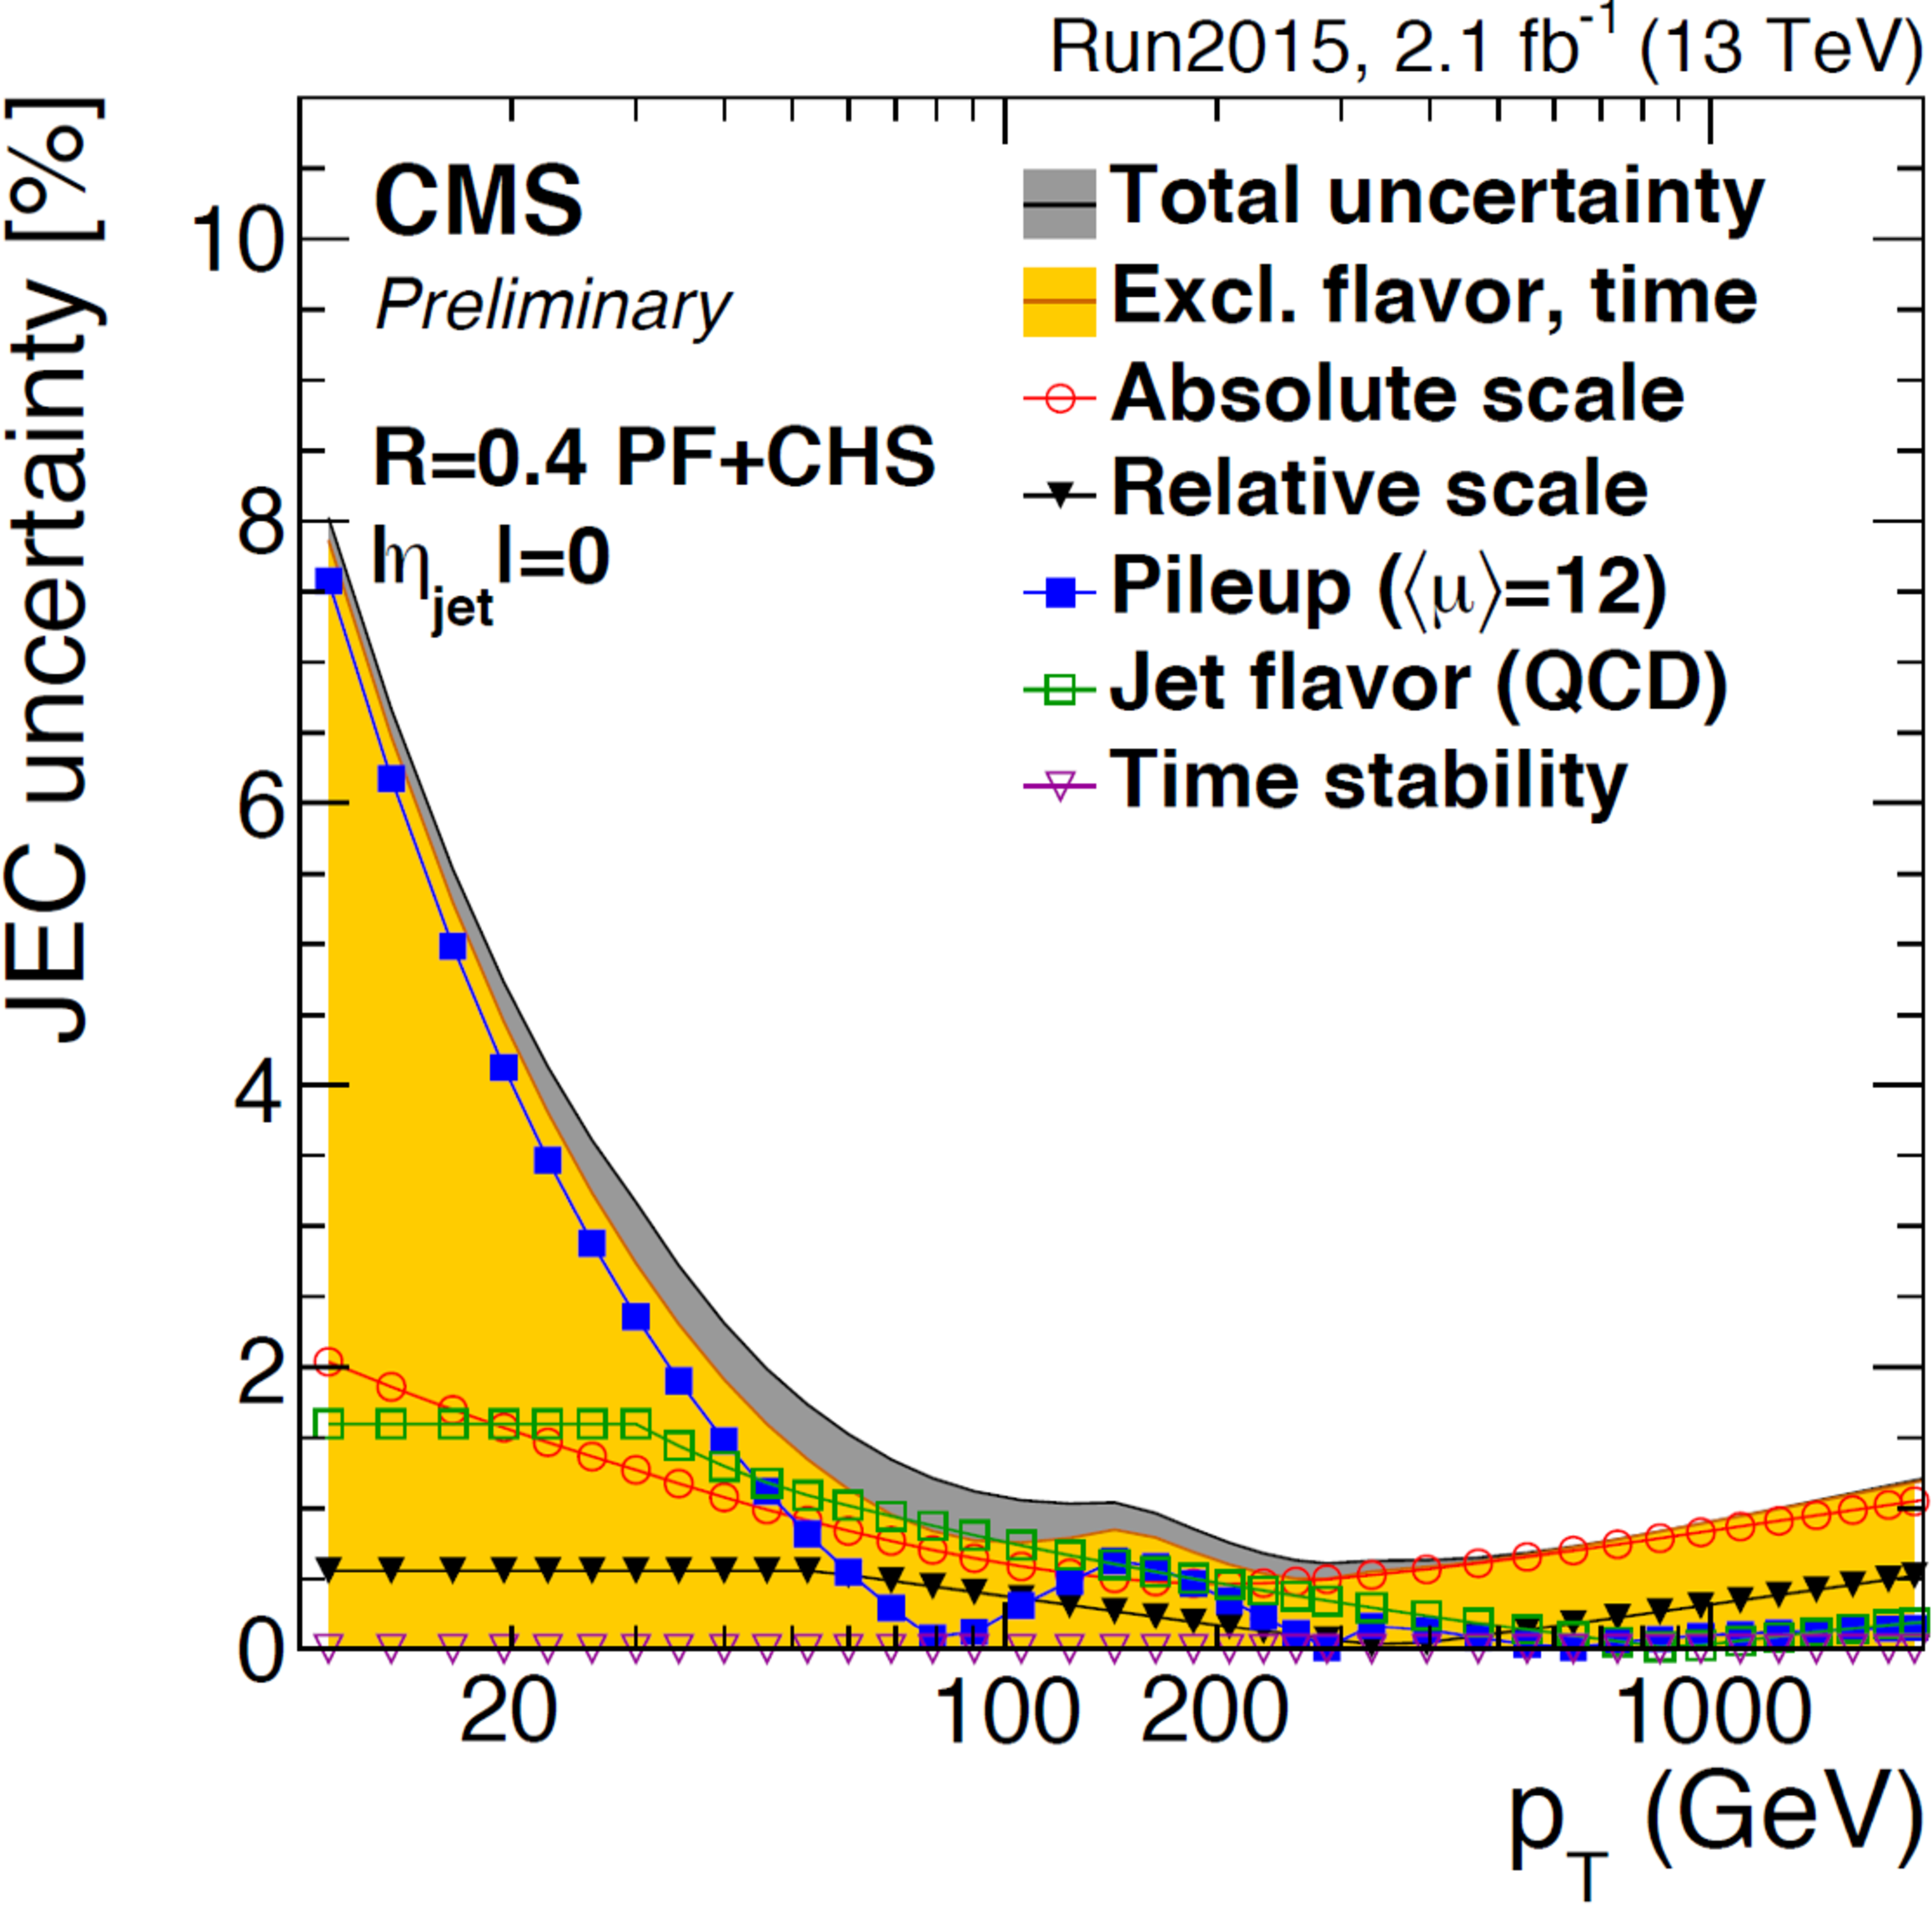
\includegraphics[width=0.45\textwidth]{images/jetUncPt.pdf}
}
\subfigure{
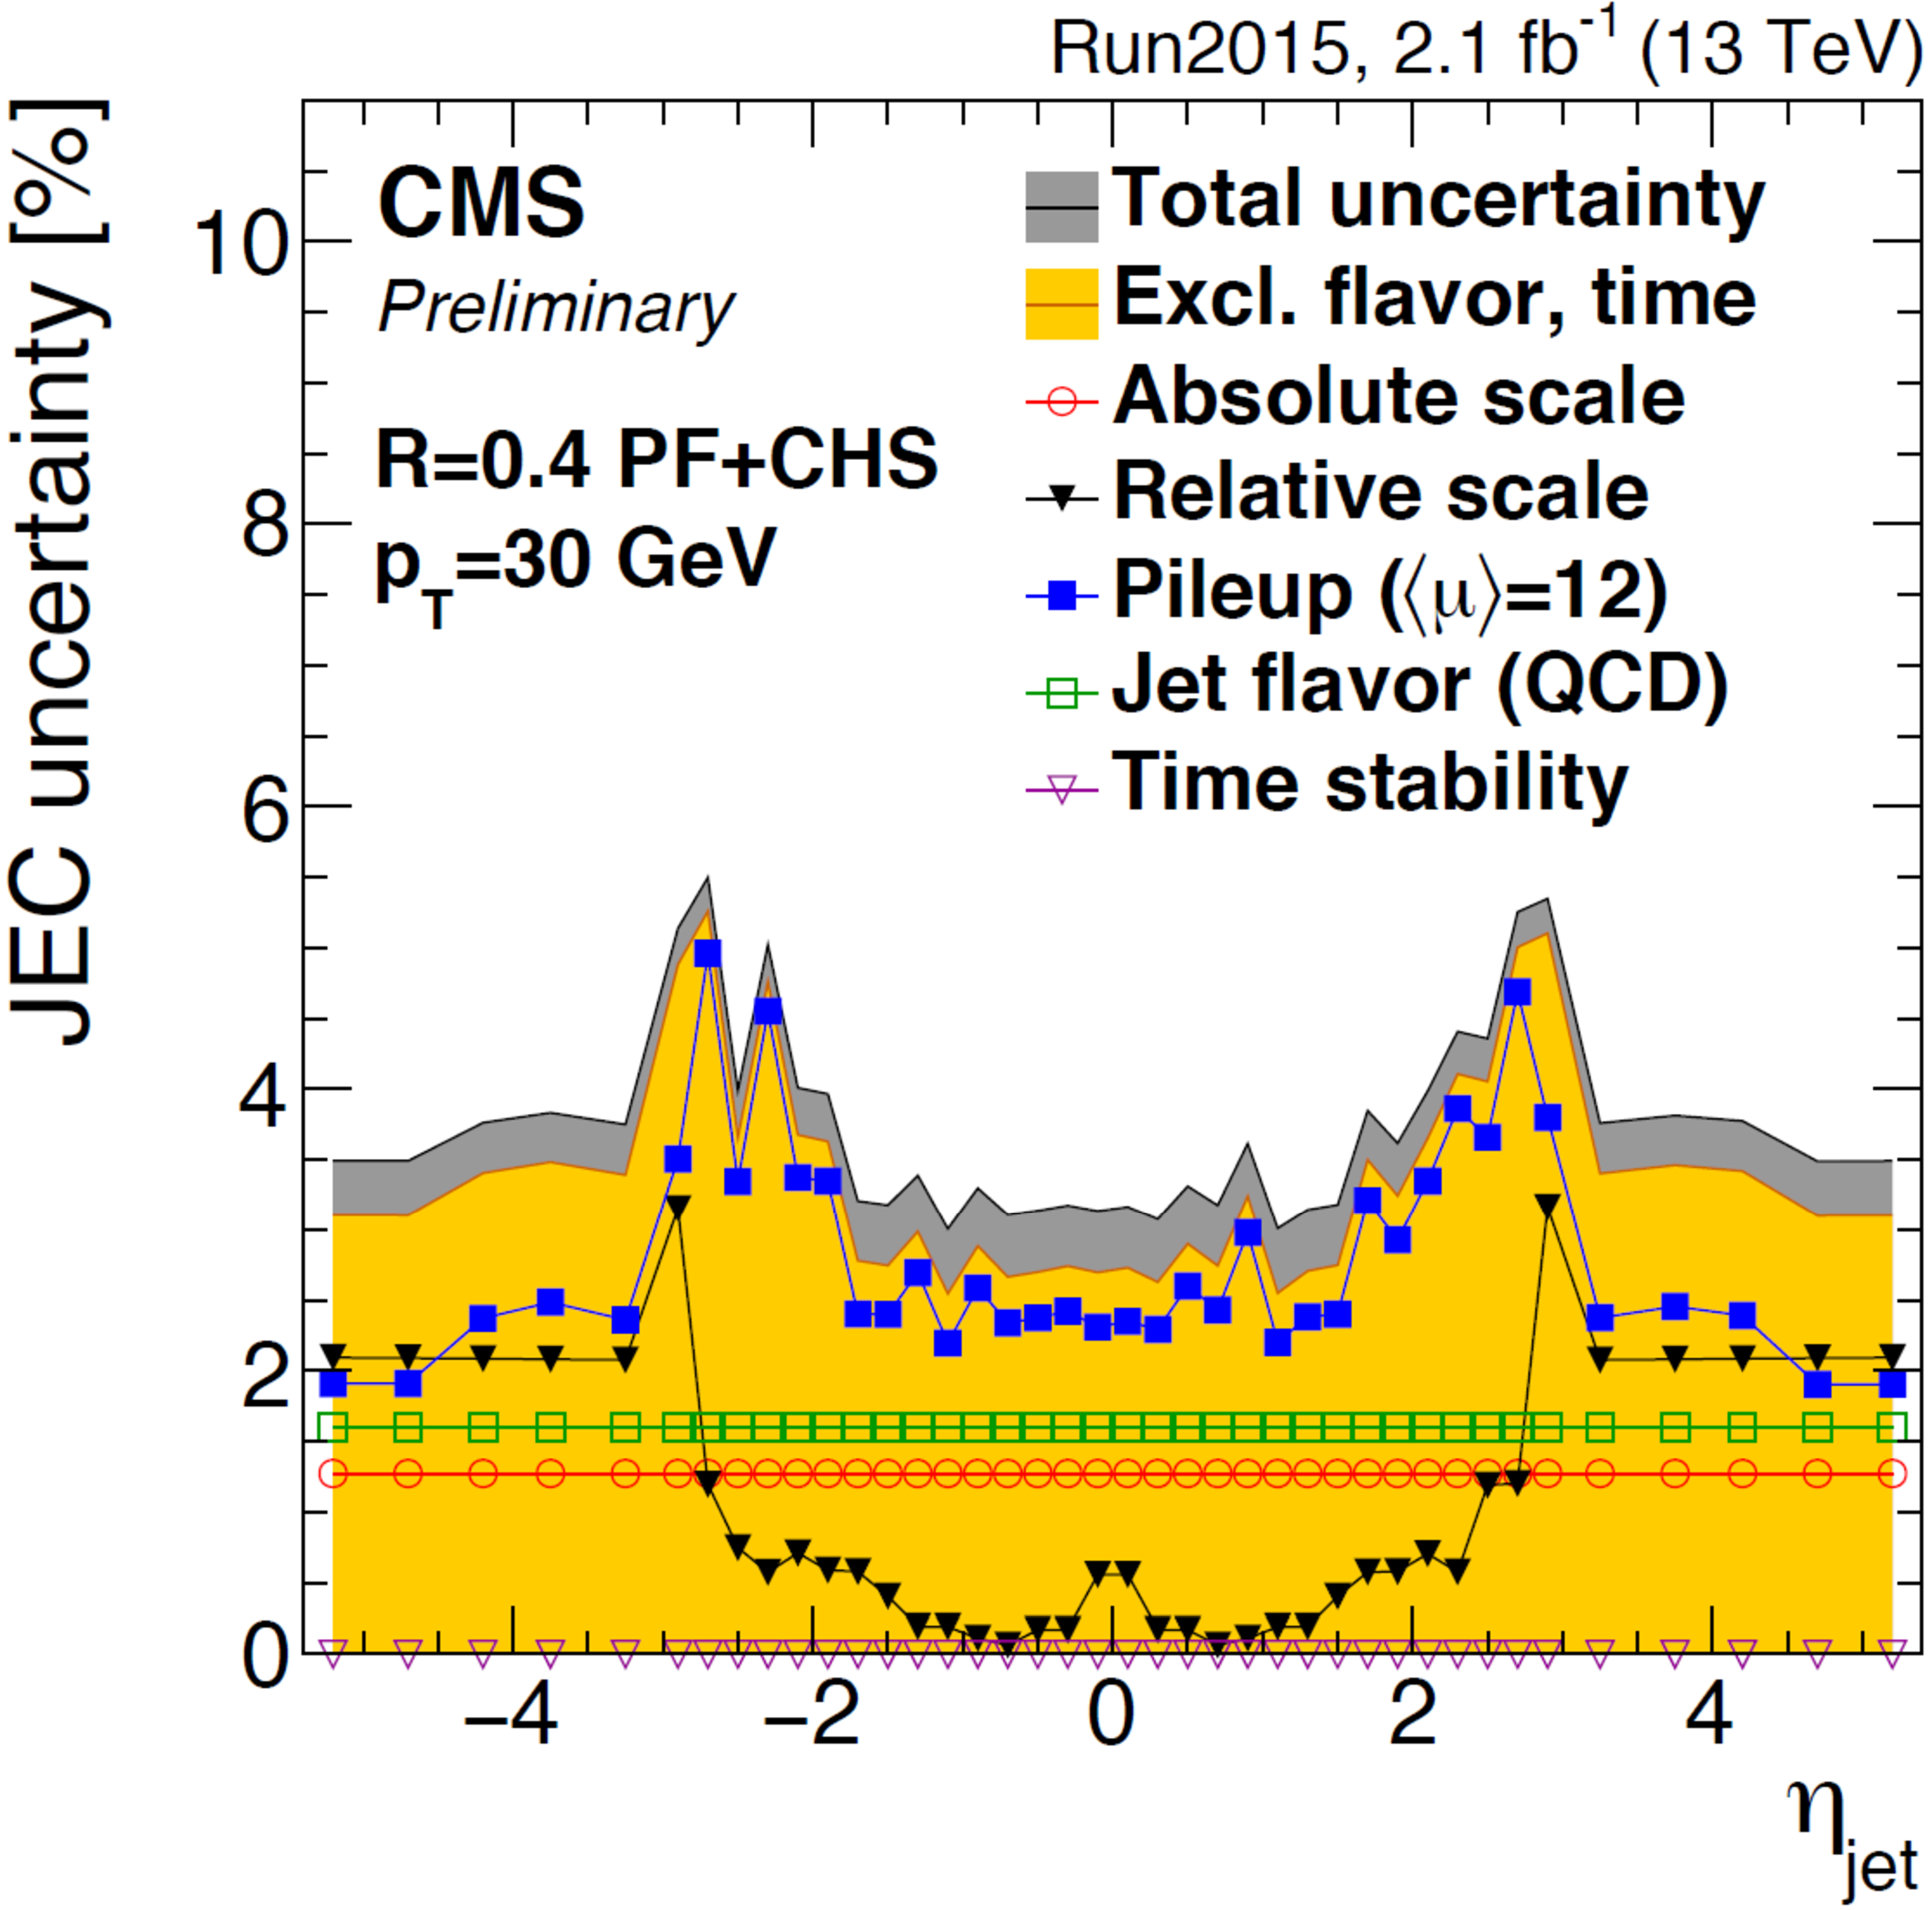
\includegraphics[width=0.45\textwidth]{images/jetUncEta.pdf}
}
\caption{JEC uncertainties as a function of \pt (left) for jets reconstructed with $\eta=0$ and as a function of $\eta$ (right) for jets with $\pt=30$\,\GeV. All jets are reconstructed with the PF technique and using the anti-$k_t$ algorithm with $R=0.4$, after applying the CHS correction. Results are based on $2.1$\,\ifb of data collected at 13\,\TeV.}\label{fig:JECunc}
\end{figure}

\subsubsection{Jet energy resolution}
Measurements show that the jet energy resolution (JER) in data is worse than in the simulation, therefore the simulated jets need to undergo a smearing procedure in order to have a better description of the data. 

Reconstructed jets in simulated events are corrected for the jet energy resolution using a two step procedure. In the first step, the reconstructed jet \pt is scaled for the observed \pt difference between reconstructed and generated jets. This method only works for reconstructed jets that are well matched to generated jets, where the matching is based on $\Delta R$ and $\Delta \pt$ requirements. For reconstructed jets that do not fulfil the matching requirements, a gaussian smearing of the \pt distribution is applied in order to obtain the desired resolution.

\textcolor{red}{jet identification?}

\section{Jet b tagging}\label{sec:btag}

Jets that arise from bottom quark hadronization (b-jets) are present in many physics processes,
such as the decay of top quarks. The ability to accurately identify b-jets is crucial to reduce the otherwise overwhelming background in channels such as \hwwllnn, which involves jets from gluons (g) and light-flavour quarks (u, d, s), as well as from c quarks fragmentation.

Algorithms for b-jets identification (also known as b tagging algorithms) exploit the long lifetime of b hadrons present in jets, originating from the hadronization of b quarks. This long lifetime results in a decay of the b hadron that is displaced with respect to the primary interaction vertex, i.e. the presence of tracks from which a secondary vertex may be reconstructed. In addition, b hadrons have a probability of around 20\% to decay to a muon or electron. Hence, also the presence of these charged leptons can be exploited for b-jets identification techniques.

A variety of reconstructed physics objects as tracks, vertices and identified leptons, can be used to build observables that discriminate between b and light quark jets. Several b tagging algorithms have been developed by CMS, each one based on different input information. A common feature of all the algorithms is that each one yields a single discriminator value for every jet, which measures the likelihood that the jet has been produced by the hadronization of a b quark. The minimum thresholds on these discriminators define loose (``L''), medium (``M''), and tight (``T'') operating points with a misidentification probability for light-parton jets close to 10\%, 1\%, and 0.1\%, respectively, at an average jet \pt of about 80\,\GeV. The misidentification probability, also known as mistag rate, is defined as the probability to wrongly identify a light-parton jet as a b-jet.

Some of the algorithms make use of the track impact parameters (IP) with respect to the primary vertex, defined as the distance between the primary vertex and the track at their point of closest approach, to distinguish the decay products of b hadrons from prompt tracks. The impact parameter has the same sign as the scalar product of the vector pointing from the primary vertex to the point of closest approach with the jet direction. Tracks originating from the decay of particles travelling along the jet axis will tend to have positive IP values. In contrast, the impact parameters of prompt tracks can have positive or negative IP values. The impact parameter significance, defined as the ratio of the IP to its estimated uncertainty, is used as an observable.

The \emph{Track Counting} (TC) algorithm sorts tracks inside a jet by decreasing values of the IP significance. Although the ranking tends to bias the values for the first track to high positive IP significances, the probability to have several tracks with high positive values is low for light-parton jets. Therefore two different versions of the algorithm use the IP significance of the second and third ranked track as discriminator value.  These two versions of the algorithm are called \emph{Track Counting High Efficiency} (TCHE) and \emph{Track Counting High Purity} (TCHP), respectively.

A general extension of the TC algorithm, the \emph{Jet Probability} (JP), combines the IP information of several tracks inside the jet, using an estimate of the likelihood that all tracks associated to the jet come from the primary vertex as a discriminating variable. A variant of
the JP algorithm also exists in which the four tracks with the highest impact parameter significance get a higher weight in the jet probability calculation. This algorithm is referred to as \emph{Jet B-Probability} (JBP).

A different approach consists in using the secondary vertices and the related kinematic variables, together with displaced tracks information, to discriminate between b- and non-b-jets. This algorithm is known as \emph{Combined Secondary Vertex} (CSV). The magnitude and direction of the vector connecting the primary and secondary vertices are used as discriminating variables and quality requirements are imposed to secondary vertex candidates. In addition, the usage of displaced tracks information allows to increase the efficiency for events where no secondary vertex is found. Several variables related to secondary vertices and displaced tracks are used to build likelihood ratios that have a good discriminating power.

Two algorithms for reconstructing secondary vertices are exploited. For the first algorithm, the
tracks associated to jets and fulfilling some quality requirements are used in the adaptive vertex reconstruction (AVR) algorithm~\cite{Waltenberger:1166320}. The AVR is the algorithm used for CMS analyses during the 8\,\TeV data taking. In contrast with this method, the Inclusive Vertex Finder (IVF) algorithm is not seeded from tracks associated to reconstructed jets, but instead makes use of all tracks in the event, with appropriate selections, to reconstruct the secondary vertices. The latter is the default algorithm used to reconstruct secondary vertices for CMS analyses using 13\,\TeV data.

A new b-jet identification algorithm has been recently developed, combining the discriminators provided by the JP and CSV algorithms with a Boosted Decision Tree (BDT) technique. This combined multivariate algorithm (cMVA) is found to slightly improve the b-jet identification efficiency.

The performance of these algorithms is determined using simulated \ttbar events, selecting events with at least one jet with $\pt > 30$\,\GeV. This is shown in Fig.~\ref{fig:btagperf}, where the b-jet identification efficiency versus the misidentification probability is reported for the various algorithms. This plot serves just as an illustration, since the b tagging performance depend on the \pt and $\eta$ distribution of the jets, and need to be checked for each analysis phase space.

\begin{figure}[htb]
\centering
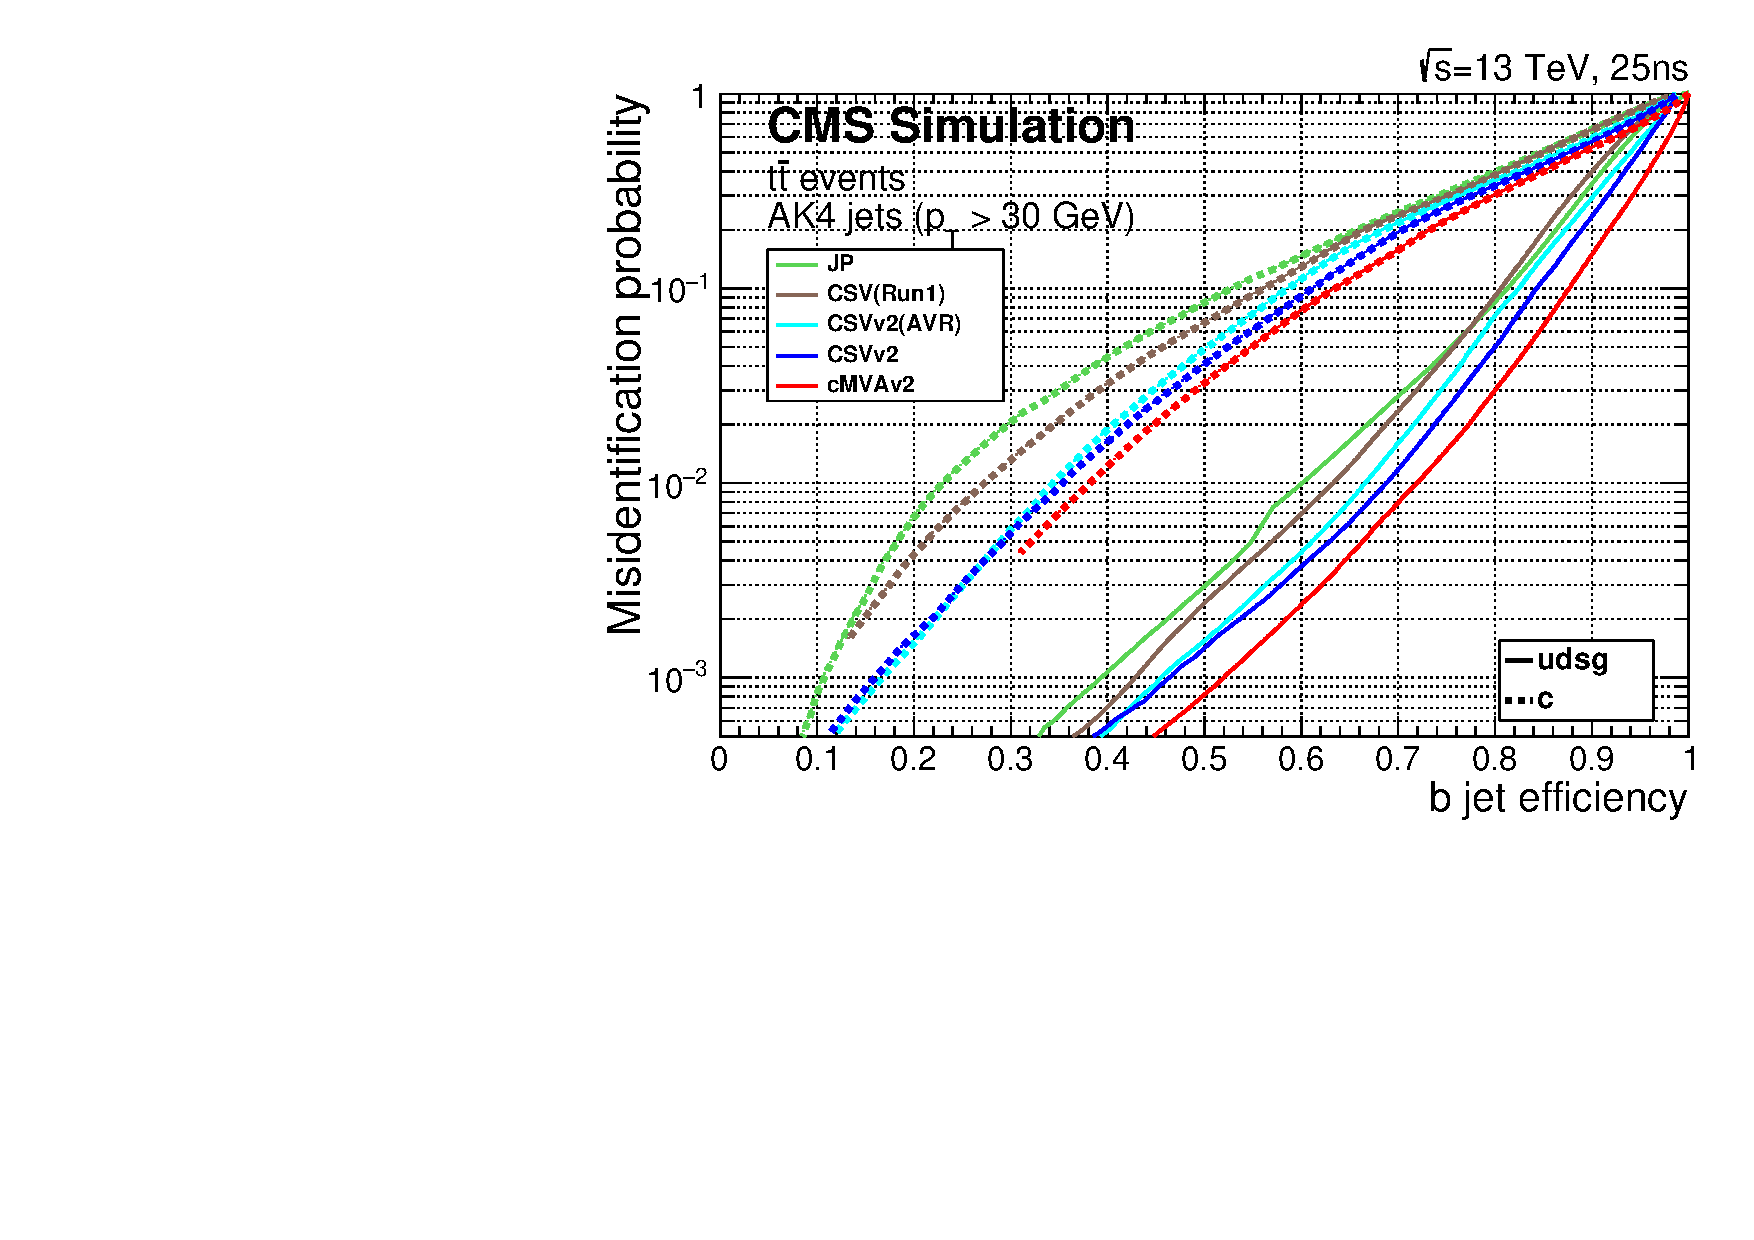
\includegraphics[width=0.7\textwidth]{images/btagperf.pdf}
\caption{Performance of the b tagging algorithms demonstrating the probability for non-b-jets to be misidentified as b-jets as a function of the efficiency to correctly identify b-jets. The curves are obtained from simulated \ttbar events using anti-$k_t$ jets clustered with $R=0.4$ and requiring $\pt>30$\,\GeV.}\label{fig:btagperf}
\end{figure}



\section{Missing transverse energy}\label{sec:met}


\cleardoublepage
\chapter{Measurement of the Higgs boson transverse momentum at 8\TeV using \hwwllnn decays}\label{chap4}

\section{Introduction}
%%%%%%%%%%%%%%%%%%%%%%%%%%%%%%%%%%%%%%%%%%%%%%%%%%%%%%%%%%%%%%%%%%%%%%
\label{sec:Introduction}

%This measurement can be used to directly inspect the perturbative QCD theory in the Higgs sector.
%In particular the \pth variable is sensitive to the Higgs production mode and the differential distribution in this variable can be used to inspect the effects of the top quark mass in the gluon fusion top loop. Moreover, any observed deviation from the SM expectation, especially in the tail of the \pth distribution, could be a hint of physics beyond the SM.

The Higgs boson production at hadron colliders is characterized by \pth and $\eta$. The $\eta$ distribution is essentially driven by the PDF of the partons in the colliding hadrons, and it is only mildly sensitive to radiative corrections. The \pth distribution is instead sensitive to QCD radiative corrections. 
Considering the ggH production mode, at LO in perturbation theory, $\mathcal{O}(\alpha_s^2)$, the Higgs boson is always produced with \pth equal to zero. Indeed in order to have \pt different from zero, the Higgs boson has to recoil at least against one parton. Higher order corrections to the ggH process are numerically large and are known at NLO including full top quark mass dependence~\cite{Spira:1995rr,Harlander:2005rq}, and at NNLO using the so-called large-$m_\mathrm{t}$ approximation~\cite{Ravindran:2003um,Catani:2007vq,Anastasiou:2015ema}, in which the top quark mass is assumed to be very large and the fermionic loop is replaced by an effective vertex of interaction. Starting from the NLO, the Higgs boson can be produced recoiling against other final state partons, resulting in a finite \pth. For this reason the LO process for Higgs production at $\pt \neq 0$ is at $\mathcal{O}(\alpha_s^3)$, and the counting of perturbative orders differs between inclusive Higgs boson production and \pth distribution. Also, NNLO QCD corrections in the \pth observable have recently been shown~\cite{Chen:2016zka}.

When $\pth \sim m_\mathrm{H}$ the QCD radiative corrections to \pth differential cross section are theoretically evaluated using fixed-order calculations. When $\pth \ll m_\mathrm{H}$ the perturbative expansion does not converge due to the presence of large logarithmic terms of the form $\alpha_s^n \ln^{2n}m_\mathrm{H}^2/\pt^2$, leading to a divergence of $d\sigma/d\pt$ in the limit of $\pt\to0$. For computing the \pth spectrum in this region soft-gluon resummation techniques are used, and matched to the fixed-order calculation in the $\pth \sim m_\mathrm{H}$ region.
For the \pth differential cross section the large-$m_\mathrm{t}$ calculation is a crude approximation, since it is known that the top quark mass has a non-negligible effect on the shape of the spectrum. Moreover the inclusion of the bottom quark contribution in the fermionic loop can significantly modify the \pth shape~\cite{Grazzini:2013mca}, as shown in Fig.~\ref{fig:pth_quarkmass}. Hence, a precise experimental measurement of the \pth spectrum is important to test the existing SM calculations. 

\begin{figure}[!h]
\centering
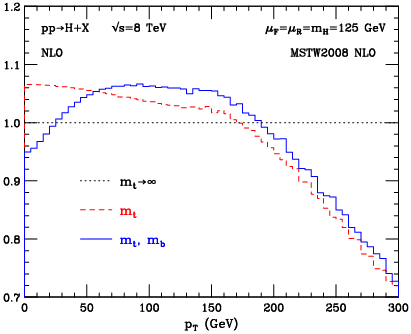
\includegraphics[width=0.5\textwidth]{images/pth_quarkmass.png}
\caption{\pth distribution computed at NLO ($\alpha_s^3$) and normalized to the calculation obtained in the large-$m_\mathrm{t}$ approximation. The red dashed line corresponds to the calculation including the top quark mass while the blue line refers to the calculation including also the bottom quark effects.}\label{fig:pth_quarkmass}
\end{figure}

Possible extensions of the SM predict a modification of the Higgs boson couplings to gluons and to the top quark. Many of these models actually predict the existence of new states that interact with the SM Higgs boson, but are beyond the direct production reach at the actual LHC energies. The effect of these new states could however show up as a deviation of the Higgs boson couplings with respect to the SM expectation. The modification of the couplings, as shown in Refs.~\cite{Azatov:2013xha,Harlander:2013oja}, can change the kinematics of the Higgs boson production and the effect can be particularly sizeable in the tail of the \pth distribution. 
Other models, such as Composite Higgs~\cite{Marzocca:2012zn}, predict the existence of top-partners, which are heavy resonances with the same quantum numbers as the top quark, that can interact with the Higgs boson in the ggH fermionic loop, changing the \pth shape with respect to what the SM predicts~\cite{Banfi:2013yoa}.
The measurement of the \pth spectrum is thus a useful tool for indirect searches of new particles predicted by theories beyond the SM.

Measurements of the fiducial cross sections and of several differential
distributions, using the $\sqrt{s}=8$\TeV LHC data, have been reported by ATLAS~\cite{Aad:2014tca,Aad:2014lwa,Aad:2015lha} and CMS~\cite{Khachatryan:2015rxa,Khachatryan:2015yvw} for the ${\mathrm{H} \to \mathrm{ZZ} \to 4\ell}$ ($\ell = \mathrm{e},\mu$) and H $\to \gamma\gamma$ decay channels. In this chapter a measurement of the fiducial cross section times branching fraction ($\sigma \times \mathcal{B}$) and \pt{} spectrum for Higgs boson production in \ensuremath{\mathrm{H}\rightarrow{}\WW\rightarrow \mathrm{e}^{\pm} \mu^{\mp}\nu\nu} ~decays, based on $\sqrt{s} = 8$\TeV LHC data, is reported.

The analysis is performed looking at different flavour leptons in the final state in order to suppress the sizeable contribution of backgrounds containing a same-flavour lepton pair originating from Z boson decay.

Although the \hwwllnn{} channel has lower resolution in the \pth{} measurement
compared to the H $\to \gamma\gamma$ and  H $\to \rm{ZZ}\to 4\ell$ channels
because of neutrinos in the final state, the channel has a significantly
larger $\sigma \times \mathcal{B}$, exceeding those for H $\to \gamma\gamma$ by a factor
of 10 and H $\to \rm{ZZ}\to 4\ell$ by a factor of 85 for a Higgs boson mass of
125\GeV~\cite{Heinemeyer:2013tqa}, and is characterized by good signal
sensitivity. Such sensitivity allowed the observation of a Higgs boson at the level of 4.3 (5.8 expected)
standard deviations for a mass hypothesis of 125.6 GeV using the full LHC data set at 7 and 8\TeV~\cite{Chatrchyan:2013iaa}.

The measurement is performed in a fiducial phase space defined by kinematic requirements on
the leptons that closely match the experimental event selection.

The effect of the limited detector resolution, as well as the
selection efficiency with respect to the fiducial phase space are corrected to
particle level with an unfolding procedure~\cite{Cowan:2002in}, as explained in Sec.~\ref{sec:Unfolding}.



%\clearpage
\section{Data sets and triggers}
%%%%%%%%%%%%%%%%%%%%%%%%%%%%%%%%%%%%%%%%%%%%%%%%%%%%%%%%%%%%%%%%%%%%%%
\label{sec:Datasets}

%-------------------------------------------------------------------------------
%\subsection{Data sets and triggers\label{subsec:Datasets}}
The data set used for this analysis corresponds to 19.4\ifb of proton-proton collisions at $\sqrt{s}=8$\TeV, collected by the CMS detector during 2012.
Only data corresponding to good data taking quality are considered.

Events are required to fire one of the unprescaled single-electron, single-muon or muon-electron triggers. Due the rather high LHC instantaneous luminosity the single-lepton triggers must have high HLT \pt thresholds, otherwise the rate of these triggers would be too large to be sustained. The double-lepton triggers allow to lower down the \pt thresholds while keeping a sustainable trigger rate, thus maintaining a good sensitivity to the Higgs boson signal, for which the lepton \pt can be rather small.
A brief overview of the HLT \pt criteria on the leptons
is given in Table~\ref{tab:trigger}. While the HLT lepton \pt thresholds of 17 and 8 \GeV for the double
lepton triggers accommodate the offline lepton \pt selection of 20 and 10 \GeV, the higher \pt thresholds
in the single lepton triggers help partially recovering double lepton trigger inefficiencies
as a high \pt lepton is on average expected due to the kinematic of the Higgs decay. 

\begin{table}[h]
\begin{center}
\caption{Transverse momentum thresholds applied in the lepton triggers at the HLT level. 
         Double set of thresholds indicates the thresholds for each leg of the double lepton triggers.}
\begin{tabular}{ccc}
\toprule
Trigger path       & Threshold \\
\midrule
Single electron    & $\pt > 27 $ \GeV         \\  
Single muon        & $\pt > 24 $ \GeV         \\ 
Muon-Electron      & $\pt > 17$ and $8 $ \GeV         \\ 
Electron-Muon      & $\pt > 17$ and $8 $ \GeV         \\ 
\bottomrule
\end{tabular}
\label{tab:trigger} 
\end{center}
\end{table}

The trigger is not simulated in MC samples but the combined trigger efficiency
is estimated from data and applied as a weight to all simulated events, as described in Sec.~\ref{sec:trigeff}.
% The trigger efficiency for single and double lepton triggers is calculated using a Tag and Probe technique separately for muons and electrons, in bins of $\eta$ and \pt.
%%%%%%%%%%%%%%%%%%%%
%%%%%%%%%%%%%%%%%%%% 

%SPOSTATO IN CAP. 2
%The Tag and Probe method uses a known mass resonance (e.g. $J/\Psi$, Z) to select particles of the desired type, and probe the efficiency of a particular selection criterion on these particles. In general the ``tag'' is an object that passes a set of very
%tight selection criteria designed to isolate the required particle type. Tags are often referred
%to as a “golden” electrons or muons and the fake rate for passing tag selection criteria should
%be very small. A generic set of the desired particle type (i.e. with potentially very loose selection criteria) known as ``probes'' is selected by pairing these objects with tags such that the
%invariant mass of the combination is consistent with the mass of the resonance. Combinatoric
%backgrounds may be eliminated through any of a variety of background subtraction methods
%such as fitting, or sideband subtraction. The definition of the probe objects depend on the
%specifics of the selection criterion being examined. The simple expression to get the efficiency $\epsilon$
%as a function of \pt and $\eta$ is given below:
%
%\begin{equation}
%\epsilon(\pt,\eta) = \frac{ N^\mathrm{probe}_\mathrm{pass}}{N^\mathrm{probe}_\mathrm{pass} + N^\mathrm{probe}_\mathrm{fail}}
%\end{equation}
%%%%%%%%%%%%%%%%%%%%%
%%%%%%%%%%%%%%%%%%%%%
%For double lepton triggers the efficiency is calculated separately for each leg of the trigger and then combined together. In the calculation the efficiencies of the two trigger legs are considered as independent, given that the correlations are very small. The combined efficiency is then used as a kinematics-dependent weight to be applied on top of simulated events.
%
%The event efficiency $\epsilon_\mathrm{ev}$ for an event with two leptons to pass the single lepton trigger is given by the following formula:
%
%\begin{equation}\label{eq:single_trigg}
%\epsilon_\mathrm{ev} = 1 - (1-\epsilon_{S,\ell1})\cdot(1-\epsilon_{S,\ell2})\quad,
%\end{equation}
%
%where $\epsilon_{S,\ell1}$ and $\epsilon_{S,\ell2}$ are the efficiencies for the leading and subleading lepton to pass the single lepton trigger. In other words, the dilepton event passes the single lepton trigger if either one of the two leptons passes the single lepton trigger, excluding the cases for which both leptons pass the trigger. For double lepton triggers, the event efficiency can be written as:
%
%\begin{equation}\label{eq:double_trigg}
%\epsilon_\mathrm{ev}  = \epsilon_{D,\ell1}^\mathrm{lead} \cdot \epsilon_{D,\ell2}^\mathrm{trail} + (  1 -  \epsilon_{D,\ell1}^\mathrm{lead} \cdot \epsilon_{D,\ell2}^\mathrm{trail})\cdot\epsilon_{D,\ell1}^\mathrm{trail} \cdot \epsilon_{D,\ell2}^\mathrm{lead} \quad,
%\end{equation}
%
%where $\epsilon_{D,\ell1}^{\mathrm{lead}(trail)}$ is the efficiency of the first lepton to pass the leading (trailing) leg of the double lepton trigger, and $\epsilon_{D,\ell2}^{\mathrm{lead}(trail)}$ is the efficiency of the second lepton to pass the leading (trailing) leg of the double lepton trigger. The final event efficiency applied to reweight the events in simulation is given by the boolean OR of the event efficiencies corresponding to the single and double lepton triggers, which, using Eqs.~\eqref{eq:single_trigg} and ~\eqref{eq:double_trigg}, can be written as:
%
%\begin{equation}
%\begin{split}
%\epsilon_\mathrm{ev} & = 1 - (1-\epsilon_{S,\ell1})\cdot(1-\epsilon_{S,\ell2}) + \\
%                     & + (1-\epsilon_{S,\ell1})\cdot(1-\epsilon_{S,\ell2}) \cdot \\
%                     & \cdot [ \epsilon_{D,\ell1}^\mathrm{lead} \cdot \epsilon_{D,\ell2}^\mathrm{trail} + (  1 -  \epsilon_{D,\ell1}^\mathrm{lead} \cdot \epsilon_{D,\ell2}^\mathrm{trail})\cdot\epsilon_{D,\ell1}^\mathrm{trail} \cdot \epsilon_{D,\ell2}^\mathrm{lead} ] \quad.
%\end{split}
%\end{equation}
%
%The term that multiplies the double lepton trigger event efficiency is needed to ensure that the events passing the double lepton trigger do not pass also the single lepton trigger.


%-------------------------------------------------------------------------------
\section{Monte Carlo samples\label{subsec:MC}}

Several Monte Carlo event generators are used to simulate the signal and background processes:
\begin{itemize}
\item the first version of the \textsc{Powheg} program (\textsc{Powheg V1}) provides event samples for the \hww signal
for the ggH and VBF production mechanisms, as well as \ttbar and tW processes~\cite{Alioli:2011as}, with NLO accuracy;
\item the VH process is simulated using \textsc{pythia 6.426}~\cite{Sjostrand:2006za};
\item the $\mathrm{qq} \to \mathrm{W^{+}W^{-}}$, Drell-Yan, ZZ, WZ, W$\gamma$, W$\gamma^*$, tri-bosons and W+jets processes are generated using
the \textsc{Madgraph 5.1.3} event generator;
\item the gg$\to \mathrm{W^{+}W^{-}}$ process is generated using the \textsc{gg2ww} 3.1 generator ~\cite{Binoth:2006mf} and its cross section is scaled to the approximate NLO prediction~\cite{Bonvini:2013jha,Passarino:2013bha}.
\end{itemize}
For samples generated at leading-order (LO) accuracy in perturbative QCD, the \textsc{cteq6l}~\cite{Lai:2010nw} set of parton distribution functions
(PDF) is used, while \textsc{ct10}~\cite{Lai:2010vv} is used for next-to-leading order (NLO) ones.
Cross section calculations at next-to-next-to-leading order (NNLO) are used for the \hww process~\cite{Dittmaier:2011ti}.
The $\hww$ process simulation is reweighted so that the \pth spectrum and inclusive production cross section closely match the SM calculations that have NNLO+NNLL QCD accuracy in the description of the Higgs boson inclusive production, in accordance with the LHC Higgs Cross Section Working Group recommendations~\cite{Heinemeyer:2013tqa}.
The reweighting of the \pth spectrum is achieved by tuning the \textsc{Powheg} generator, as described in detail in Ref.~\cite{Alioli:2010xd}.
Cross sections computed with NLO QCD accuracy are used for the background processes~\cite{Heinemeyer:2013tqa}.
The contribution of the \ttH production mechanism is checked to be negligible (below 1\%) in the whole \pth spectrum and is not included in the analysis. In Fig.~\ref{fig:signal_comp} the relative fraction of the four production mechanisms is shown for each \pth bin.

\begin{figure}[htb]
\centering
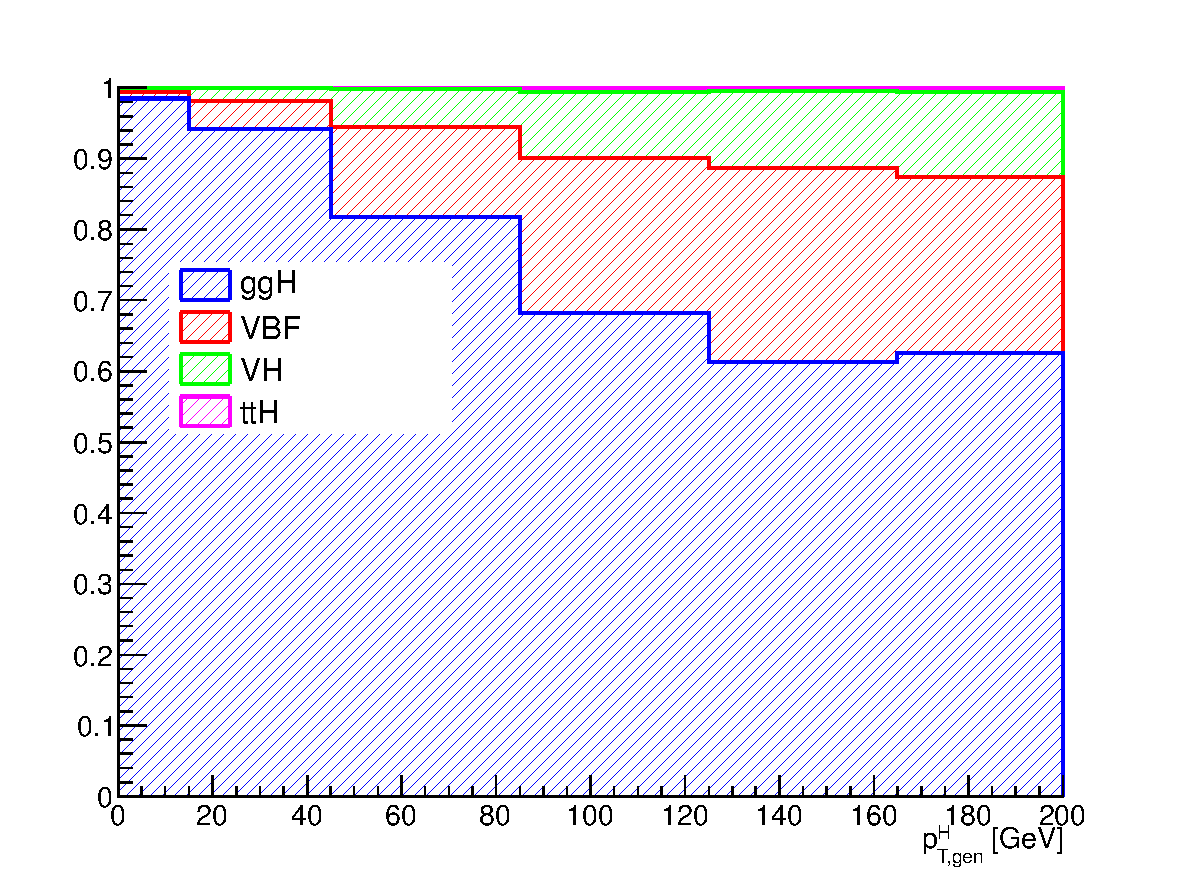
\includegraphics[width=0.7\textwidth]{images/signal_composition_ttH.pdf}
\caption{Relative fraction of ggH, VBF, VH and \ttH in each bin of the Higgs boson transverse momentum.}\label{fig:signal_comp}
\end{figure}

For all processes, the detector response is simulated using a detailed description of the CMS detector, based on the \textsc{Geant4} package~\cite{Agostinelli:2002hh}.

Minimum bias events are superimposed on the simulated events to emulate the additional 
proton-proton interactions per bunch crossing. The pile-up multiplicity in simulated events has been generated poissonianly sampling from a distribution similar to the one expected from data.
The simulated events are reweighted to correct for observed differences between data and simulation in the number of pile-up events, as shown in Fig.~\ref{fig:nvertices}.

\begin{figure}[htb]
\centering
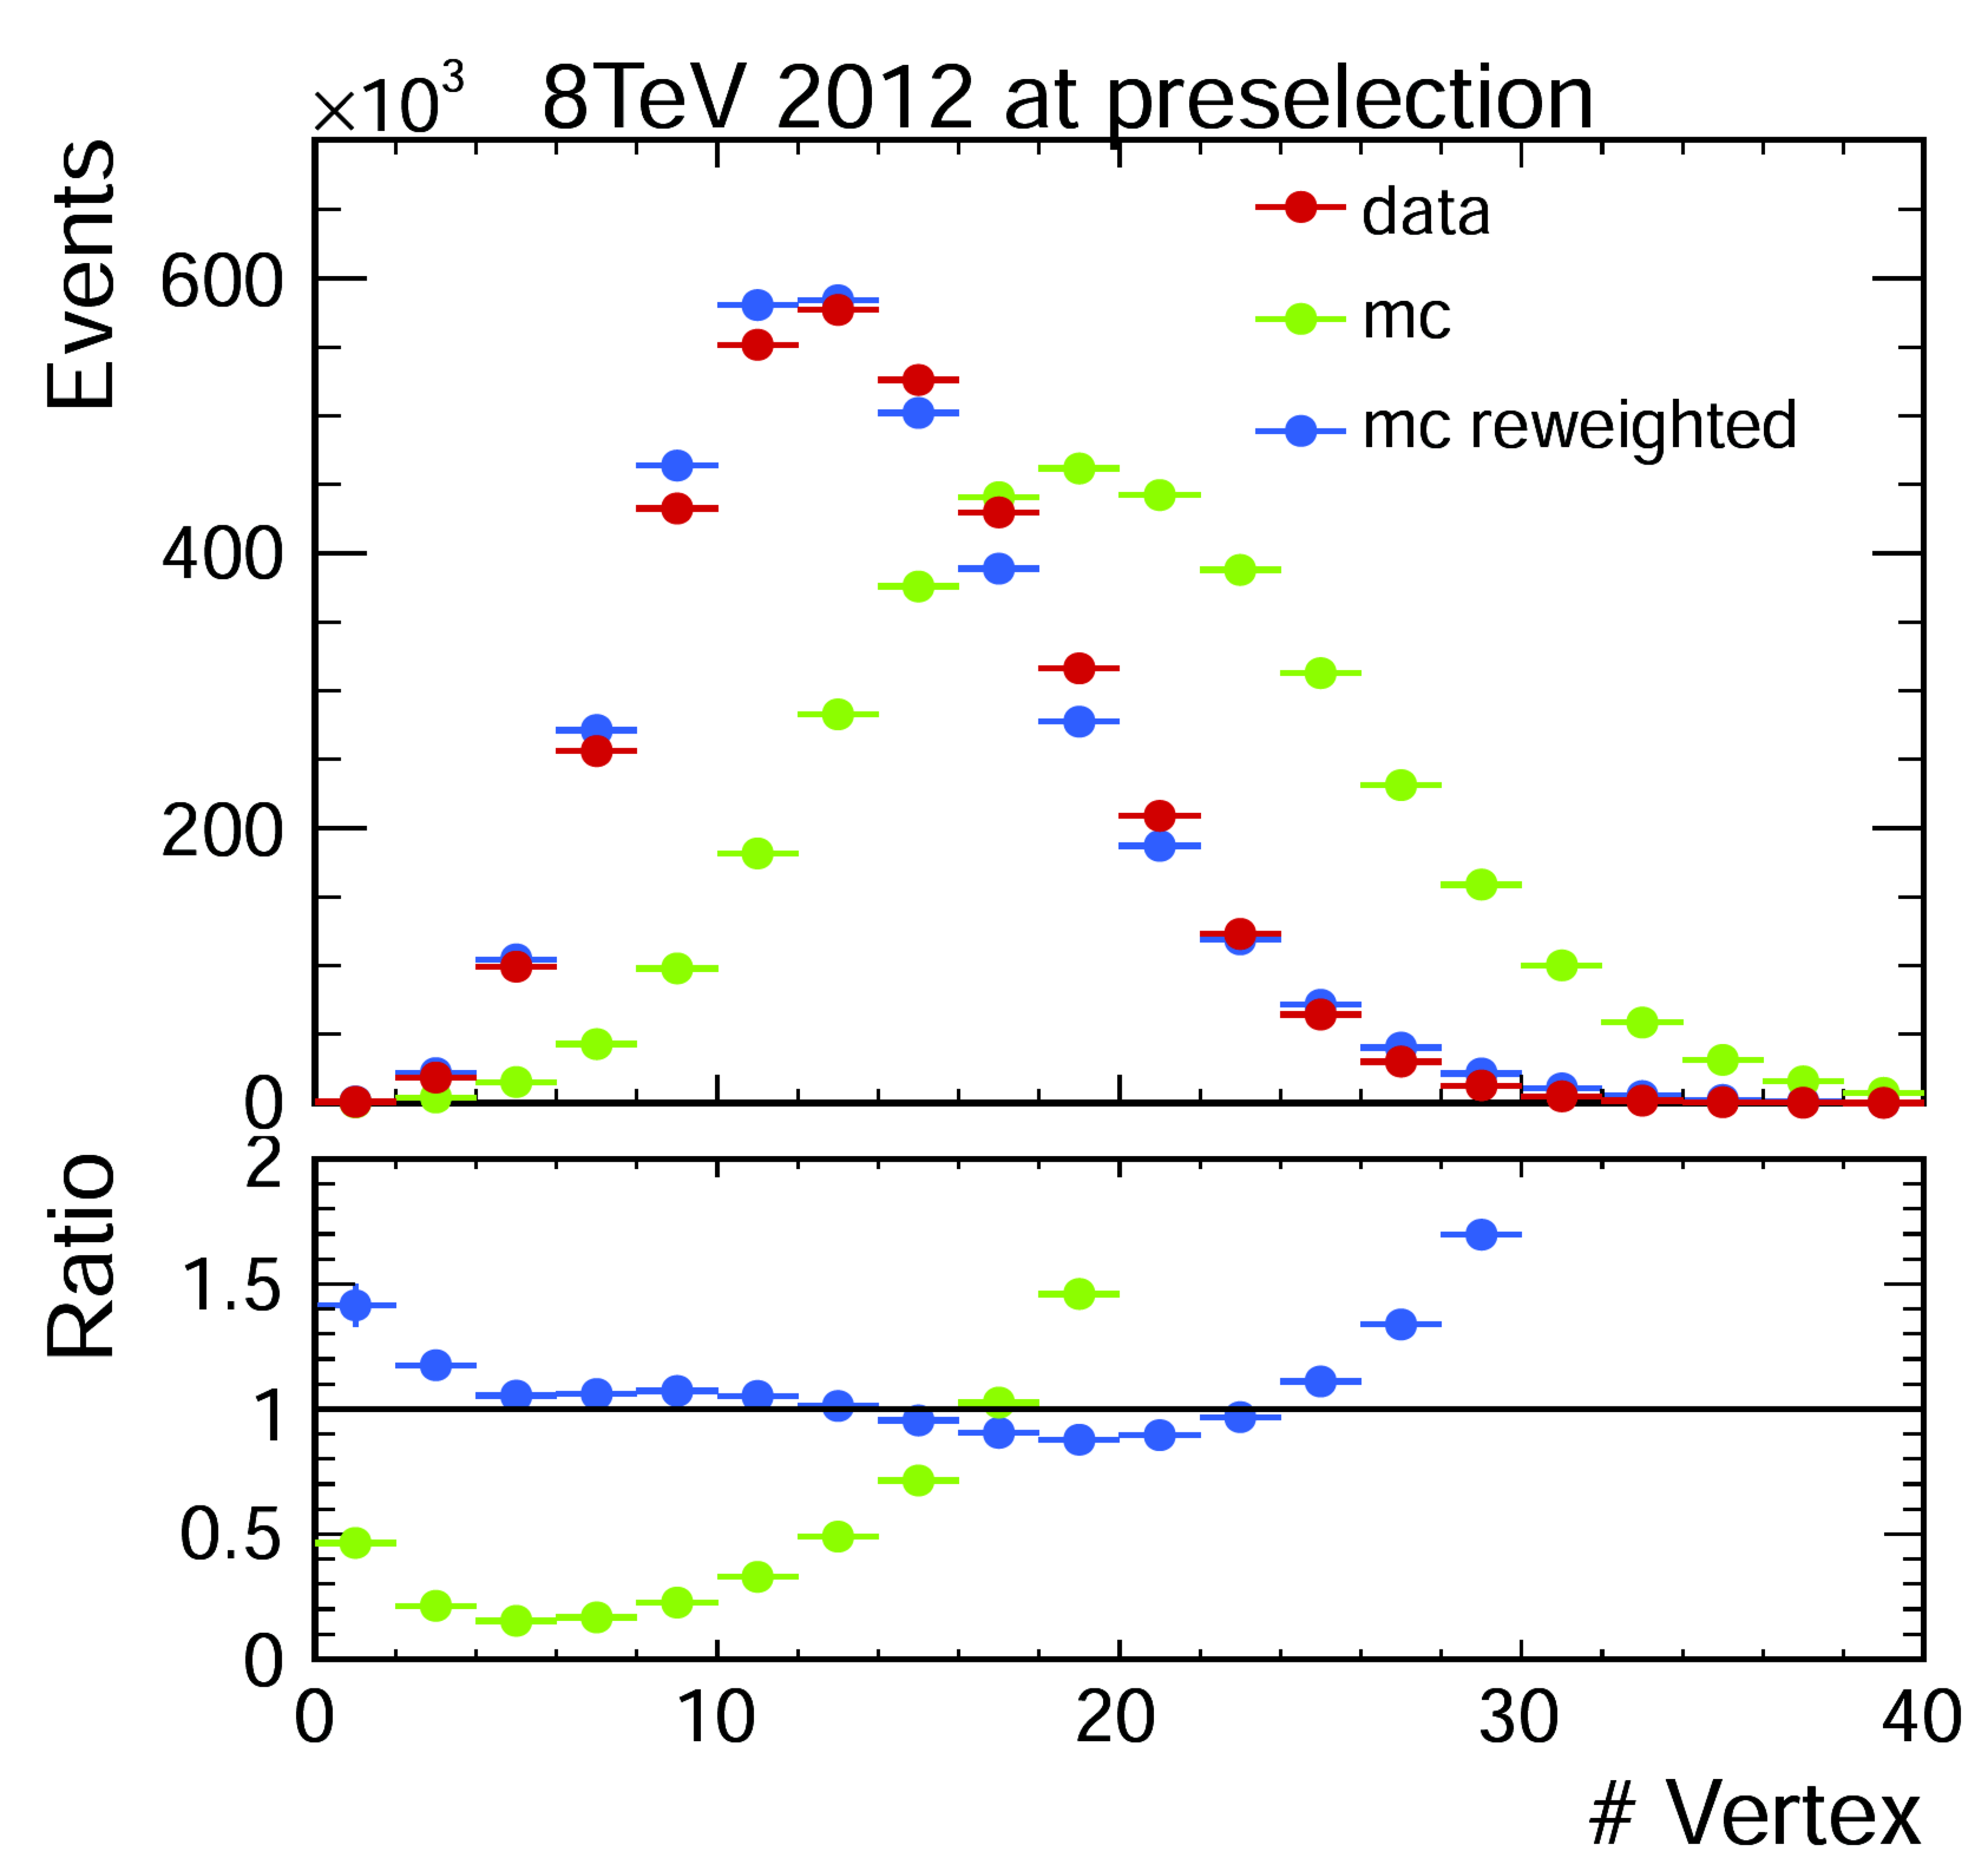
\includegraphics[width=0.7\textwidth]{images/nvertex.pdf}
\caption{Distribution of the number of vertices in data and simulation, before and after applying the pile-up reweighting.}\label{fig:nvertices}
\end{figure}

For the comparison of the measured unfolded spectrum with the theoretical predictions, two additional MC generators are used for simulating the SM Higgs boson production in the ggH process: \textsc{HRes} 2.3~\cite{deFlorian:2012mx,Grazzini:2013mca} and the second version of the \textsc{Powheg} generator (\textsc{Powheg V2})~\cite{Bagnaschi:2011tu}.
\textsc{HRes} is a partonic level MC generator that computes the SM Higgs
boson cross section at NNLO accuracy in QCD and performs the NNLL
resummation of soft-gluon effects at small \pt. The central predictions of
\textsc{HRes} are obtained including the top and bottom quark mass contribution to
the gluon fusion loop, fixing the renormalization and factorization scale central values at a Higgs boson mass of 125\GeV. The cross section normalization is scaled, to take into account electroweak corrections (by a factor of 1.05) and effects of threshold resummation (by a factor of 1.06)~\cite{Actis:2008ug,Catani:2003zt}. The upper and lower bounds of the uncertainties are obtained by scaling up and down both the renormalization and the factorization scales by a factor of two.
The \textsc{Powheg V2} generator is a matrix element based generator that provides a NLO description of the ggH process in association with zero jets, taking into account the finite mass of the bottom and top quarks.
The \textsc{Powheg} prediction is tuned using the \textsc{Powheg} damping factor \textit{hdump} of 104.17~\GeV, in order to match the \pth{} spectrum predicted by \textsc{HRes} in the full phase space. This factor reduces the emission of additional jets in the high \pt regime, and enhances the contribution from the Sudakov form factor in the limit of low \pt.
The \textsc{Powheg} generator is interfaced to the \textsc{JHUGen} generator version 5.2.5~\cite{Gao:2010qx,Bolognesi:2012mm,Anderson:2013afp} for the decay of the Higgs boson to a W boson pair and interfaced with \textsc{Pythia 8}~\cite{Sjostrand:2007gs} for the simulation of parton shower and hadronization effects.

%\clearpage
\section{Analysis Strategy}
%%%%%%%%%%%%%%%%%%%%%%%%%%%%%%%%%%%%%%%%%%%%%%%%%%%%%%%%%%%%%%%%%%%%%%
\label{sec:AnalysisStrategy}

The analysis presented here is based on that used in the previously published \hwwllnn{}
measurements by CMS~\cite{Chatrchyan:2013iaa}, modified to be inclusive in the number of jets. 
This modification significantly reduces the uncertainties related to the modelling of the number of jets produced in association with the Higgs boson.

The signal contribution is extracted performing a template binned likelihood fit, using the two-dimensional (\mll,\mt) shape for each background and signal process, as described in Sec.~\ref{sec:SignalExtraction}.

\textcolor{red}{controllare se mll e mT sono già stata definite}

\subsection{Event reconstruction and selections}\label{sec:Selections}

Electrons and muons used in the analysis are reconstructed using the PF technique as described in Sec.~\ref{sec:leptonID}. In particular, muon candidates are required to be identified both as Tracker Muons and Global Muons.

\begin{comment}
The electron selection is based on two multivariate discriminants, one specialised in identifying the electron object and the other for isolation. The cut value for each discriminant is optimised to provide a good fake electron rejection and to improve the signal acceptance.

Muons are reconstructed using the standard CMS selection and are required to be identified both in the tracker (\textit{Tracker Muon}) and in the muon chambers (\textit{Global Muon}). Additionally quality criteria on the muon track are required, such as to have at least 10 hits in the tracker (at least one of which in the pixel detector) and to have $\chi^2/ndf < 10$.
Muon isolation is based on the Particle-Flow algorithm. An MVA approach is considered, based on the radial distributions of the Particle-Flow candidates inside a cone of radius 0.5 around the muon direction.

The efficiencies for the identification and isolation of the electrons and muons are measured in data and in simulation selecting a pure sample of leptons coming from the Z$\to\ell\ell$ decay, and using a Tag and Probe technique very similar to the one described in Sec.~\ref{subsec:Datasets} for the trigger efficiency. In this case, the probe lepton is defined by loose isolation and identification requirements and the efficiency to pass the tight analysis selections is measured performing a simultaneous fit of signal plus background in two categories, corresponding to events in which the probe lepton pass or fail the analysis requirements. For the electrons, the resonant signal contribution in the fit is modelled as the convolution of a Breit-Wigner and a Crystal-Ball function. A polynomial function is added to take into account the tail in the low mass region. For muons the signal is fitted using the sum of two Voigtian functions. For both electrons and muons the background contribution is modelled as a third order Bernstein polynomial function.
The efficiencies for data and simulation are extracted as parameters of the fit and are used as scale factors to correct the MC simulation to precisely model the data.
\end{comment}

Jets are reconstructed using the standard PF algorithm and using the anti-$k_t$ clustering algorithm with $\mathrm{R} = 0.5$, as described in Sec.~\ref{sec:jets}. If not specified otherwise, jets considered for jet counting are the ones with $\pt > 30$\,\GeV.

In addition to the standard CMS PF \MET, in this analysis a \textit{projected} \MET variable is also used. The \textit{projected} \MET is defined as the component of \ptmiss transverse to the nearest lepton if the lepton is situated within the azimuthal angular window of $\pm \pi/2$ from the \ptmiss direction, or the \MET itself otherwise.
Since the \MET resolution is degraded by pileup, the minimum of two projected \MET variables is used: one constructed from all identified particles (full projected \MET), and another constructed from the charged particles only (track projected \MET).

Background events from \ttbar and tW production are rejected applying a soft-muon veto and b tagging veto. The soft-muon algorithm is designed to identify muons from b quark decays. Events containing a muon satisfying the following requirements are rejected by the soft-muon veto: 
\begin{itemize}
\item reconstructed as TrackerMuon;
\item number of hits in the Silicon Tracker greater than 10;
\item transverse impact parameter less than 0.2\,cm;
\item relative isolation greater than 0.1 for muons with $\pt>20$\,\GeV.
\end{itemize}

The b tagging veto rejects events that contain jets identified as b-jets using two different algorithms for high and low \pt jets (see Sec.~\ref{sec:btag}). For jets with \pt between 10 and 30\GeV, the TCHE algorithm is applied. Low-\pt jets passing the TCHE discriminant threshold of 2.1 are tagged as b-jets.
For jets with $\pt>30$\GeV, a better performing algorithm, JP, is used. Jets are identified as b-jets by the JP algorithm if the discriminating variable has a value above 1.4.
In the following, a b tagged jet is defined as a jet, within $|\eta|<2.4$ (b-tagging requires the tracker information), and with a value of the discriminating variable above the mentioned thresholds for the two algorithms.


%%% Event selection
The event selection consists of several steps. The first step is to select \WW-like events applying a selection that consists of the following set of cuts:
\begin{enumerate}
\item {\bf Lepton preselection}:
  \begin{itemize}
  \item two opposite charge and different flavour (e$\mu$) isolated leptons reconstructed in the event;
  \item $|\eta|<2.5$ for electrons and $|\eta|<2.4$ for muons;
  \item $\pt>20\GeV$ for the leading lepton. For the trailing lepton, the transverse momentum is required to be larger than 10\GeV.
  \end{itemize}
\item {\bf Extra lepton veto}: the event is required to have two and only two leptons with opposite charge passing the lepton selection.
\item {\bf \MET preselection}: particle flow \MET is required to be greater than 20\GeV.
\item {\bf projected \MET selection}: minimum projected \MET required to be larger than 20\GeV.
\item {\bf Di-lepton mass cut}: $\mll > 12$\GeV in order to reject low mass resonances and QCD backgrounds.
\item {\bf Di-lepton \pt cut}: $\ptll > 30$\GeV to reduce the contribution of W+jets and DY to $\tau\tau$ backgrounds.
\item {\bf Transverse mass}: $\mt>60$\GeV to reject DY to $\tau\tau$ events. 
\end{enumerate}
The requirement of different flavour leptons in the final state is important in order to suppress the sizeable contribution of backgrounds containing a same flavour lepton pair originating from Z boson decay.

Events surviving these requirements are dominantly those where a top quark-antiquark pair is produced and both W bosons, which are part of the top quark decay chain, decay leptonically (dileptonic \ttbar).
Two different selections are used depending on the number of jets in the event. This is done to suppress the top quark background both in the low \pth region, where 0-jets events have the largest contribution, and for higher \pth values where also larger jet multiplicity events are important.
The selection for 0-jets events relies on the soft-muon veto and on a soft jet (with $\pt < 30$\GeV) b tagging veto.
The latter requirement exploits the TCHE algorithm to reject soft jets that are likely to come from b quarks hadronization.

For events with a jet multiplicity greater or equal than one, a different selection is applied. In this case we exploit the good b tagging performances of the JP tagger to reject all the jets with $\pt > 30$\GeV that are likely to come from b quarks hadronization. The analysis selection requires to have no events containing b-tagged jets with $\pt > 30$\GeV.

\begin{figure}[htb]
\centering
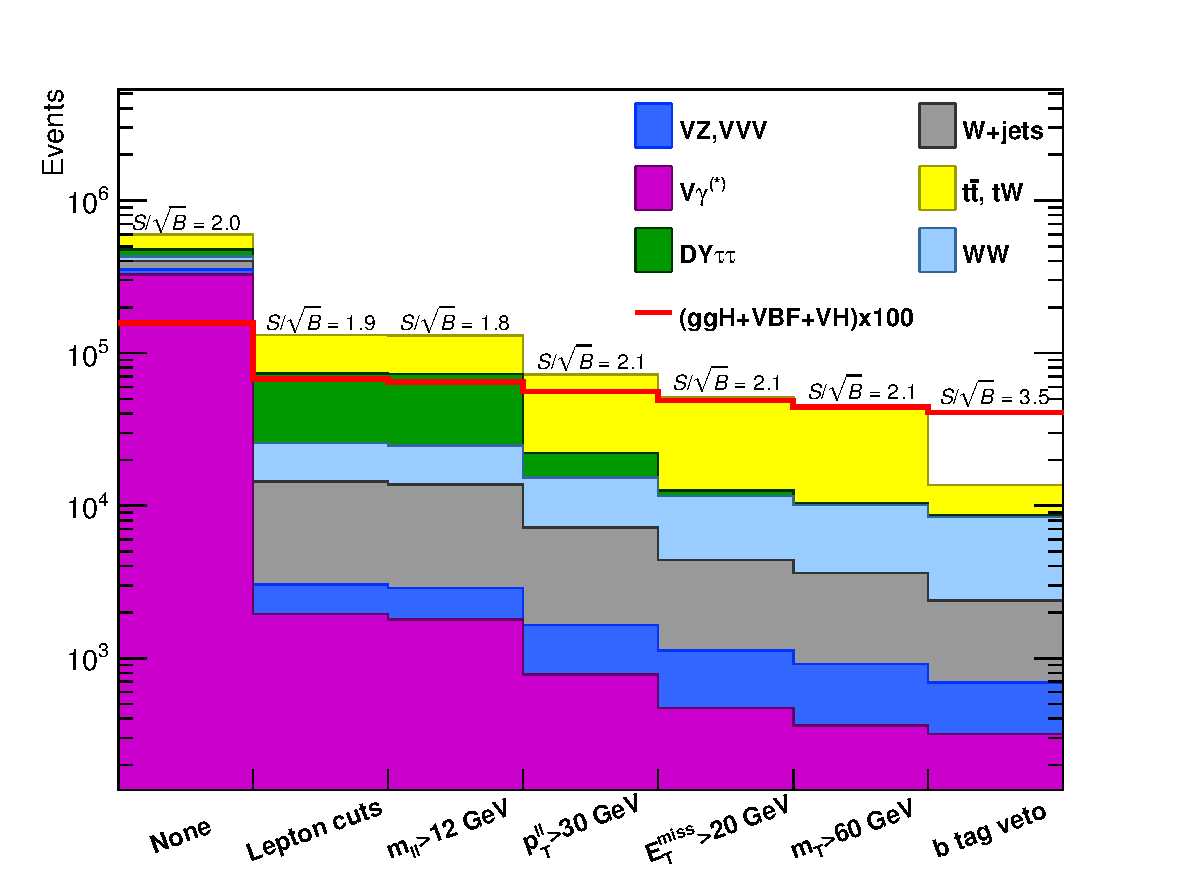
\includegraphics[width=0.8\textwidth]{images/cutflow-thesis.pdf}
\caption{Effect of selection cuts on simulated samples. The signal (red line) is multiplied by 100 and superimposed on stacked backgrounds. In each bin, corresponding to a different selection, is reported the expected number of events in MC at a luminosity of $19.46~\mathrm{fb}^{-1}$.}\label{fig:cutflow}
\end{figure}

A cut-flow plot is reported in Fig.~\ref{fig:cutflow}, showing the effect of each selection using signal and background simulations. In the first bin, labelled as ``No cut'', no selection is applied and the bin content corresponds to the total expected number of events with a luminosity of $19.4~\mathrm{fb}^{-1}$. All the events in this bin have at least two leptons with a loose transverse momentum cut of 8\GeV. In the following bin the lepton cuts are applied, including the requirement to have two opposite sign and different flavour leptons and the extra lepton veto. Then all the other selections are progressively reported, showing the effect of each cut on the background and signal yields. For each selection the expected signal over background ratio is also shown, which, after the full selection requirements, reaches a maximum value of about $3\%$.




\subsection{Simulation efficiencies and scale factors}\label{sec:ScaleFactors}

The efficiencies for the identification and isolation of the electrons and muons are measured in data and simulation selecting a pure sample of leptons coming from the Z$\to\ell\ell$ decay, and using the Tag and Probe technique described in Sec.~\ref{sec:lepIdIsoEff}. The efficiencies for data and simulation are used as scale factors to correct the simulated events to precisely model the data.

The trigger efficiency is measured in data and applied to simulation as explained in Sec.~\ref{sec:trigeff}.

The efficiency of b tagging algorithms is not well simulated by MC generators and discrepancies can occur with respect to the data. For this reason is important to measure the b tagging efficiency and the misidentification probability for the given algorithms both in data and simulation, and to correct the simulated events using scale factors. This affects not only the top quark background estimation, but also the other backgrounds and the signal. As an example, if a light-parton jet in a signal event was misidentified as a b-jet, this event would be rejected by the b-jet veto.

In this analysis, the b tagging efficiency and the misidentification probability are measured both in data and simulation, selecting a control sample enriched in b-jets, and using a Tag and Probe technique similar to the one described in Sec.~\ref{sec:lepIdIsoEff}. Below is described the method used to estimate the efficiency of the JP b tagging algorithm, but it is extendible to any other algorithm.

The control sample is defined selecting the events that pass the selections listed in Sec.~\ref{sec:Selections}, and have at least two jets with \pt greater than 30 \GeV. If the leading jet has a JP discriminator values above the threshold of 0.5, it is considered a \emph{tag}, and the sub-leading jet is the \emph{probe}. In order to avoid any bias that could arise from the probe being always the sub-leading jet, the pair is tested also in reverse order, i.e. sub-leading jet is tested against the \emph{tag} selection, and in case it passes, then the leading jet is used as \emph{probe} forming an independent \emph{tag-probe} pair. If the \probe jet has a discriminator value above the threshold used in the analysis, i.e. $>1.4$, then the \tp pair is called a \tpp pair. Otherwise it is identified as a \tfp pair.

If the \tg selection was sufficient to suppress any non top quark event, one could estimate the efficiency by dividing the number of \tp pairs in which the \probe passes the analysis JP requirement by the total number of \tp pairs. However this is not the case, since the contamination due to other background sources is not negligible. In order to estimate the efficiency in the presence of background, a variable that discriminates between true b-jets and other jets in a \ttbar sample is needed. This variable is the \pt of the \probe jet. For real b-jets this variable has a peak around 60\GeV, while it has a broad distribution for other types of jets.

The efficiencies are estimated performing a $\chi^{2}$ simultaneous fit of the \probe \pt spectrum in two different categories: one containing events with a \tpp pair and the other containing events with a \tfp pair. The normalisations in the two categories are linked by the following formulas:

\begin{equation}
\begin{split}
N_\mathrm{TPP} &= N_\mathrm{s} \varepsilon_\mathrm{s} + N_\mathrm{b} \varepsilon_\mathrm{b} \\
N_\mathrm{TFP} &= N_\mathrm{s} (1 -\varepsilon_\mathrm{s}) + N_\mathrm{b} ( 1 - \varepsilon_\mathrm{b}) \quad,
\end{split}
\end{equation}

where:
\begin{itemize}
\item $N_\mathrm{TPP}$ is the number of \tpp pairs;
\item $N_\mathrm{TFP}$ is the number of \tfp pairs;
\item $N_\mathrm{s}$ is the number of \tp pairs in which the \probe is a b-jet;
\item $N_\mathrm{b}$ is the number of \tp pairs in which the \probe is not a b-jet;
\item $\varepsilon_\mathrm{s}$ is the efficiency to identify a b-jet, i.e. the b tagging efficiency;
\item $\varepsilon_\mathrm{b}$ is the probability to misidentify a non b-jet as a b-jet, i.e. the misidentification probability\footnote{In these naming convention, the subscript ``s'' stays for ``signal'', since the b-jets represent the signal in this method. Similarly, the ``b'' subscript stays for ``background'', identifying the cases where the \probe is not a b-jet}.
\end{itemize}

The \pt shapes of the \probe jet used in the fit are taken from simulation, where the real flavour of the jet is known, both for the \tpp and \tfp categories. To check the consistency of the fitting procedure, a closure test fitting the simulation itself has been performed.
The result of the fit on MC simulation is shown in Fig.~\ref{fig:mc_tp}. The relevant efficiencies are:
\begin{equation}
\begin{split}
\varepsilon_\mathrm{s}^\mathrm{MC} &= 0.766\pm0.007 \\
\varepsilon_\mathrm{b}^\mathrm{MC} &= 0.208\pm0.015 \quad .
\end{split}
\end{equation}
These values are consistent with the true value of the b tagging efficiency in simulation. The true value is computed by selecting jets that are matched within a cone of $\Delta{R}<0.5$ with a generator level b quark, and counting the fraction of those that have a JP discriminator above threshold of 1.4. This check also assures that the \tp method does not introduce any bias within the simulation statistic accuracy.

\begin{figure}[htb]
\centering
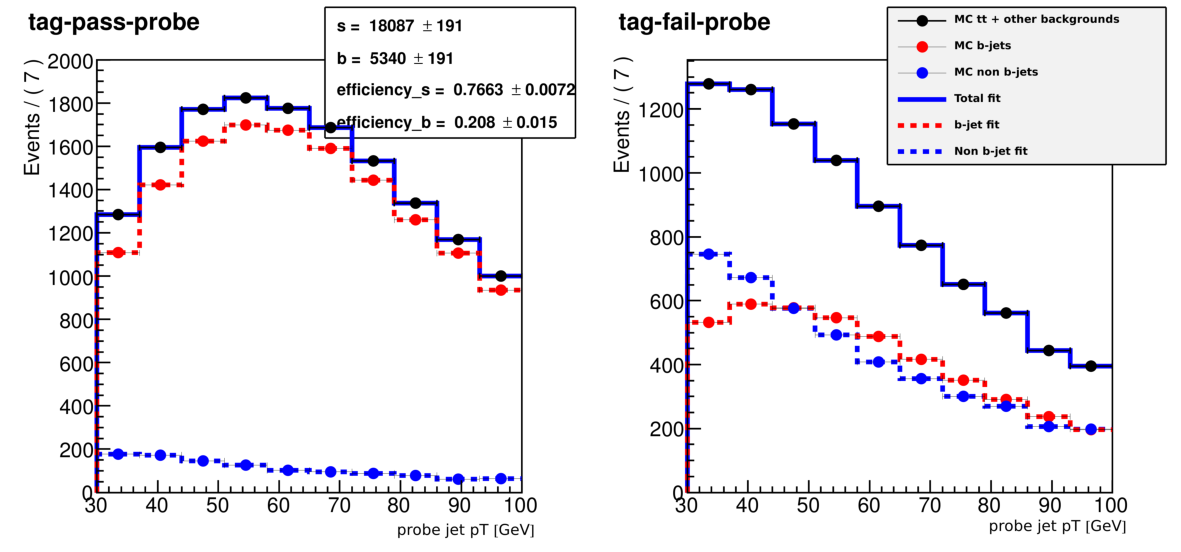
\includegraphics[width=0.8\textwidth]{images/mc_pt_probe-v2.pdf}
\caption{Simultaneous fit of the \tpp and \tfp pairs in the MC.\label{fig:mc_tp}}
\end{figure}

In order to assess the robustness of the fit, 5000 toy simulated samples have been generated with a statistics equivalent to the one expected in data and the same fit is performed. All the 5000 fit succeeded, and the pull distributions for $\varepsilon_{\rm s}$ and $\varepsilon_{\rm b}$ parameters are shown in Fig.~\ref{fig:pullstp}. The distributions represent the \emph{pull} of the efficiencies measured in the fit, where the pull variable for each toy $i$ is defined as:

\begin{equation}
pull(\varepsilon_{\rm s (b)}) = \frac{\varepsilon_{\rm s (b)}^{\rm true} - \varepsilon_{\rm s (b)}^{i}}{\sigma(\varepsilon_{\rm s (b)}^{i})} \quad,
\end{equation}

where $\sigma(\varepsilon_{\rm s (b)}^{i})$ is the uncertainty on the efficiency extracted from the fit. The pull distributions are centred on zero and have $\sigma$ close to one, as expected.

Before running the fit on data, the shapes used in the fit have been validated. To do so, a very pure phase space enriched in b jets has been defined by selecting events containing exactly two jets with a JP discriminator greater than 1.5 and no additional b-tagged jets, rejecting also events containing jets with \pt smaller than 30 \GeV. On this very pure sample, data have been compared against the shape used to fit the true b-jets in the \tpp distribution. The result is shown in Fig.~\ref{fig:purett} and shows good agreement within uncertainties.

\begin{figure}[htb]
\centering
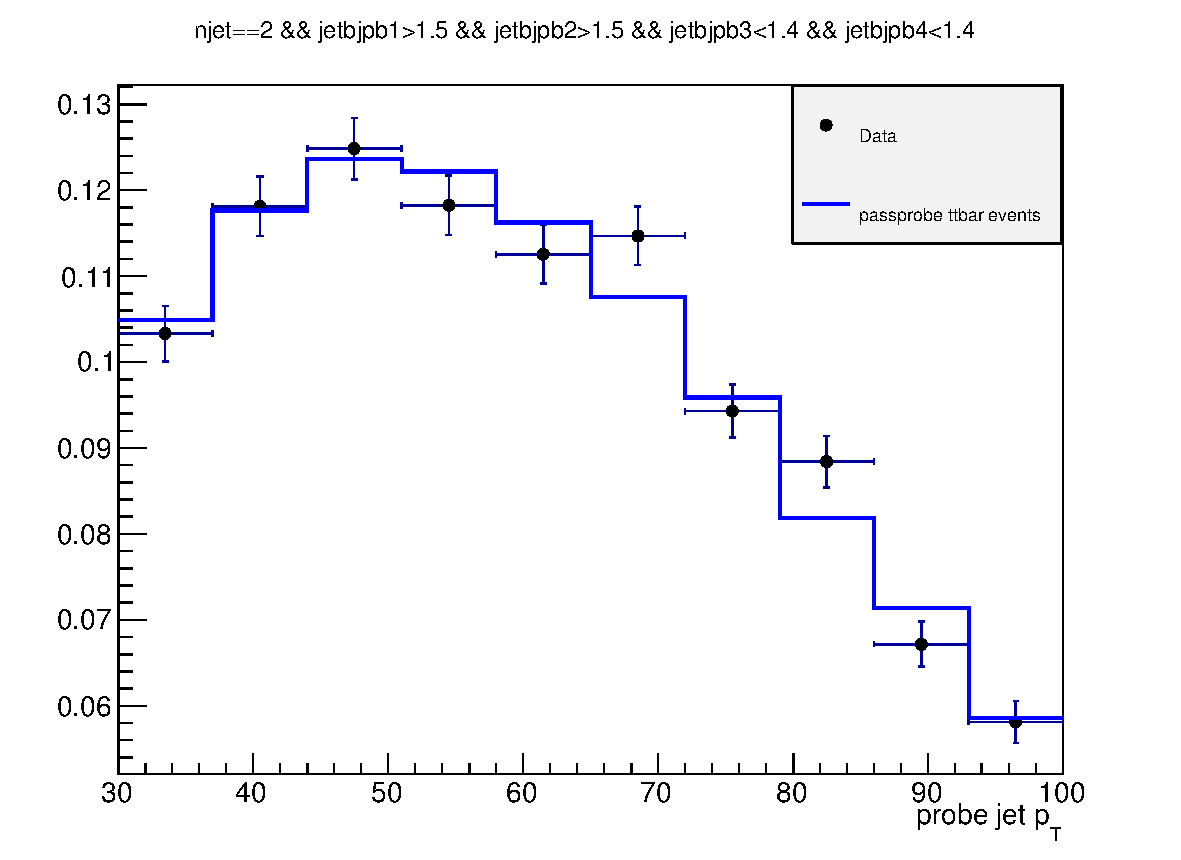
\includegraphics[width=0.6\textwidth]{images/passprobe_data_mc.pdf}
\caption{Shape comparison for the \pt spectrum of the \probe jet in data and simulation in a very pure phase space enriched in b-jets.\label{fig:purett}}
\end{figure}

Finally the fit has been performed on data, as shown in Fig.~\ref{fig:data_tp}, providing the following efficiencies:

\begin{equation}
\begin{split}
\varepsilon_\mathrm{s}^\mathrm{Data} &= 0.77\pm0.02\\
\varepsilon_\mathrm{b}^\mathrm{Data} &= 0.12\pm0.05
\end{split}
\end{equation}

\begin{figure}[htb]
\centering
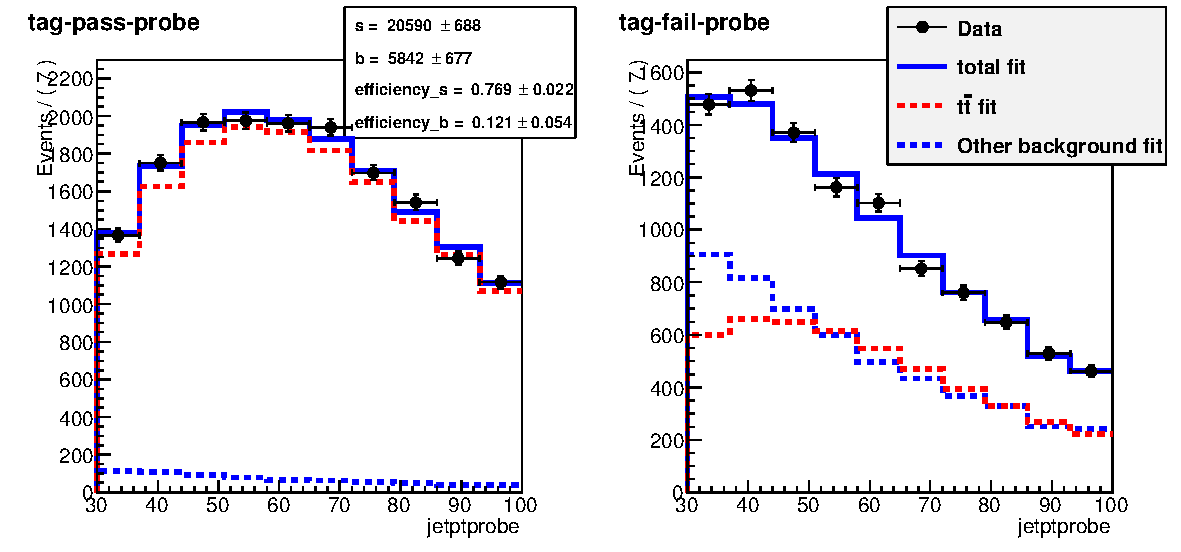
\includegraphics[width=0.8\textwidth]{images/data_ptprobe.pdf}
\caption{Simultaneous fit of the \tpp and \tfp pairs in data.\label{fig:data_tp}}
\end{figure}

Further studies have been performed to assess the effect of the relative uncertainty on the \ttbar and tW event fractions. The same procedure described above has been applied to different simulation templates obtained varying the \ttbar and tW fractions within theoretical uncertainties, and the effect on the parameters extracted with the fit procedure is found to be well below the fit uncertainties.

The ratio of the efficiency measured in data and simulation represents a per-jet scale factor that can be used to reweight the simulated events. The weights to be applied event-by-event depend on the particular jet configuration in the events itself. For the signal region ($SR$), in which a b tagging veto is required, the event weight to be applied is given by:

\begin{equation}
w_{SR} = \prod_{N_\mathrm{b-jets}} \left( \frac{1-\varepsilon_\mathrm{s}^\mathrm{Data}}{1-\varepsilon_\mathrm{s}^\mathrm{MC}} \right) \prod_{N_\mathrm{non~b-jets}} \left( \frac{1-\varepsilon_\mathrm{b}^\mathrm{Data}}{1-\varepsilon_\mathrm{b}^\mathrm{MC}} \right) \quad ,
\end{equation}

where $N_\mathrm{b-jets}$ and $N_\mathrm{non~b-jets}$ are the number of true b-jets and the number of non b-jets in the simulated event, respectively. This weight is valid if the a b tagging veto is applied. If instead the b tagging veto is reverted, also the event weight has to be modified. This is done, for example, when one wants to define a \ttbar enriched control region ($CR_{\ttbar}$) for the purpose of measuring the contribution of this background in a phase space orthogonal to the signal region. One simple way to define this control region is to require the leading jet in the event to be b-tagged. Therefore, the simulated events falling in this category must be reweighted using the following weight:

\begin{equation}
w_{CR_{\ttbar}} = 
\begin{cases}
\varepsilon_\mathrm{s}^\mathrm{Data}/\varepsilon_\mathrm{s}^\mathrm{MC},& \text{if the leading jet is a b-jet} \\
\varepsilon_\mathrm{b}^\mathrm{Data}/\varepsilon_\mathrm{b}^\mathrm{MC},& \text{if the leading jet is not a b-jet} 
\end{cases}
\end{equation}




\subsection{Fiducial phase space}\label{sec:fid_space}
The Higgs boson transverse momentum is measured in a fiducial phase space, whose definition is chosen in order to minimize the dependence of the measurements on the underlying model of the Higgs boson production and decay properties.

The exact requirements are determined by considering the two following correlated quantities: the reconstruction efficiency for signal events originating from within the fiducial phase space (fiducial signal efficiency $\varepsilon_{\rm{fid}}$), and the ratio of the number of reconstructed signal events that are from outside the fiducial phase space (``out-of-fiducial'' signal events) to the number from within the fiducial phase space. The requirement of having a small fraction of out-of-fiducial signal events, while at the same time preserving a high value of the fiducial signal efficiency $\epsilon_{\rm{fid}}$, leads to fiducial requirements at the generator level on the low-resolution variables, \MET and \mt, that are looser with respect to those applied in the reconstructed event selection.

The fiducial phase space used for the cross section measurements is defined at the particle level by the requirements given in Table~\ref{table:fid_cuts}. The leptons are defined as Born-level leptons, i.e. before the emission of final-state radiation (FSR), and are required not to  originate from leptonic $\tau$ decays. The effect of including FSR is found to modify $\epsilon_{\rm{fid}}$ at most of about 5\%.
For the VH signal process, the two leptons are required to originate from the \hwwllnn decays in order to avoid including leptons coming from the associated W or Z boson.

\begin{table}[htb]
\caption{Summary of requirements used in the definition of the fiducial phase space.}\label{table:fid_cuts}
\begin{center}
\begin{tabular}{l r}\hline\hline
\bf{Physics quantity} & \bf{Requirement} \\
\hline
Leading lepton \pt & $\pt > 20$\GeV \\
Subleading lepton \pt & $\pt > 10$\GeV \\
Pseudorapidity of electrons and muons & $|\eta| < 2.5$ \\
Invariant mass of the two charged leptons & $\mll > 12$\GeV \\
Charged lepton pair \pt & $p_{\rm T}^{\ell\ell} > 30$\GeV \\
Invariant mass of the leptonic system in the transverse plane & $m_{\rm T}^{\ell\ell \nu\nu} > 50$\GeV \\
\MET & $\MET>0$ \\
\hline
\end{tabular}
\end{center}
\end{table}

A detailed description of the fiducial region definition and its optimization is given in appendix \ref{app:fiducial_region}.










\subsection{Binning of the \pth distribution}

Experimentally, the Higgs boson transverse momentum is reconstructed as the vector sum of the lepton momenta in the transverse plane and \MET.
\begin{equation}
\vec{p}_\mathrm{T}^\mathrm{~H} = \vec{p}_\mathrm{T}^{~\ell\ell} + \vec{p}_\mathrm{T}^\mathrm{~miss}
\end{equation}
Compared to other differential analyses of the Higgs cross section, such as those in the ZZ and $\gamma\gamma$ decay channels, this analysis has to cope with the limited resolution due to the \MET entering the transverse momentum measurement.
The effect of the limited \MET resolution has two main implications on the analysis strategy: the first one is that the choice of the binning in the \pth{} spectrum needs to take into account the detector resolution; the second implication is that migrations of events across bins are significant and an unfolding procedure needs to be applied to correct for selection efficiencies and bin migration effects.

Given these aspects, the criterion that is used to define the \pth bin size is devised to keep under control the bin migrations due to the finite resolution.
For any given bin $i$, the purity $P_i$ of the signal sample is defined as the number events that are generated and also reconstructed in that bin, i.e. $N_i^\mathrm{GEN|RECO}$, divided by the number of events reconstructed in the same bin, $N_i^\mathrm{RECO}$:

\begin{equation}
P_i = \frac{N_i^\mathrm{GEN|RECO}}{N_i^\mathrm{RECO}} \quad .
\end{equation}

The bin width is chosen in such a way as to make the smallest bins able to ensure a purity of about 60\%, based on a ggH simulated sample.
Following this prescription, the whole \pth range is dividedin the following six bins: \mbox{[0--15]\GeV}, \mbox{[15--45]\GeV}, \mbox{[45--85]\GeV}, \mbox{[85--125]\GeV}, \mbox{[125--165]\GeV}, \mbox{[165--$\infty$]\GeV}.

The fiducial signal efficiency $\varepsilon_\mathrm{fid}$ and the fraction of out-of-fiducial signal events, $f_\mathrm{out-of-fid}$, are different in each \pth bin and depend on the definition of the fiducial phase space. In Fig.~\ref{fig:sel_eff} the $\varepsilon_\mathrm{fid}$ and $f_\mathrm{out-of-fid}$ parameters are shown in each \pth bin for different definitions of the fiducial phase space. In particular, they have been evaluated adding the requirements reported in Table~\ref{table:fid_cuts} in sequence, starting from a fiducial phase space defined just by the lepton \pt and $\eta$ selections, together with the different flavour requirement, and adding each time an additional selection until the full fiducial phase space in obtained. In this way, the effect of every single selection (or group of selections) on $\varepsilon_\mathrm{fid}$ and $f_\mathrm{out-of-fid}$ can be assessed. Since the variables related to leptons are measured with good resolution, the effect of including the related selections in the fiducial phase space is to increase $\varepsilon_\mathrm{fid}$ keeping $f_\mathrm{out-of-fid}$ constant. Instead, the effect of including low-resolution variables, such ad \mt, is to increase both $\varepsilon_\mathrm{fid}$ and $f_\mathrm{out-of-fid}$. Nevertheless, the $f_\mathrm{out-of-fid}$ parameter is different from zero even if only lepton cuts are taken into account. This is ascribable to two different aspects: the first one is that in the fiducial definition electrons and muons are required not to originate from $\tau$ decays; the second one is instead related to the VH production mechanism, i.e. to the fact that leptons coming from the associated boson are not included.

%The efficiency of the analysis selection with respect to the fiducial phase space is reported in Fig.~\ref{fig:sel_eff} (a) for each \pth bin. The efficiency denominator is the number of events that are inside the fiducial phase space, while the numerator is the number of events that pass both the analysis and the fiducial phase space selections. The fake rate, defined by the ratio of signal events that pass the analysis selection but are not within the fiducial phase space, divided by the total number of events passing both the analysis and the fiducial phase space selections is shown in Fig.~\ref{fig:sel_eff} (b). For both the selection efficiency and the fake rate, all the signal production mechanisms are included.
The overall values integrating over \pth are $\varepsilon_\mathrm{fid}=0.362\pm{0.005}$ and $f_\mathrm{out-of-fid}=0.126\pm0.004$ respectively, where only statistical uncertainties are taken into account.

\begin{figure}[htb]
\centering
\subfigure[]{
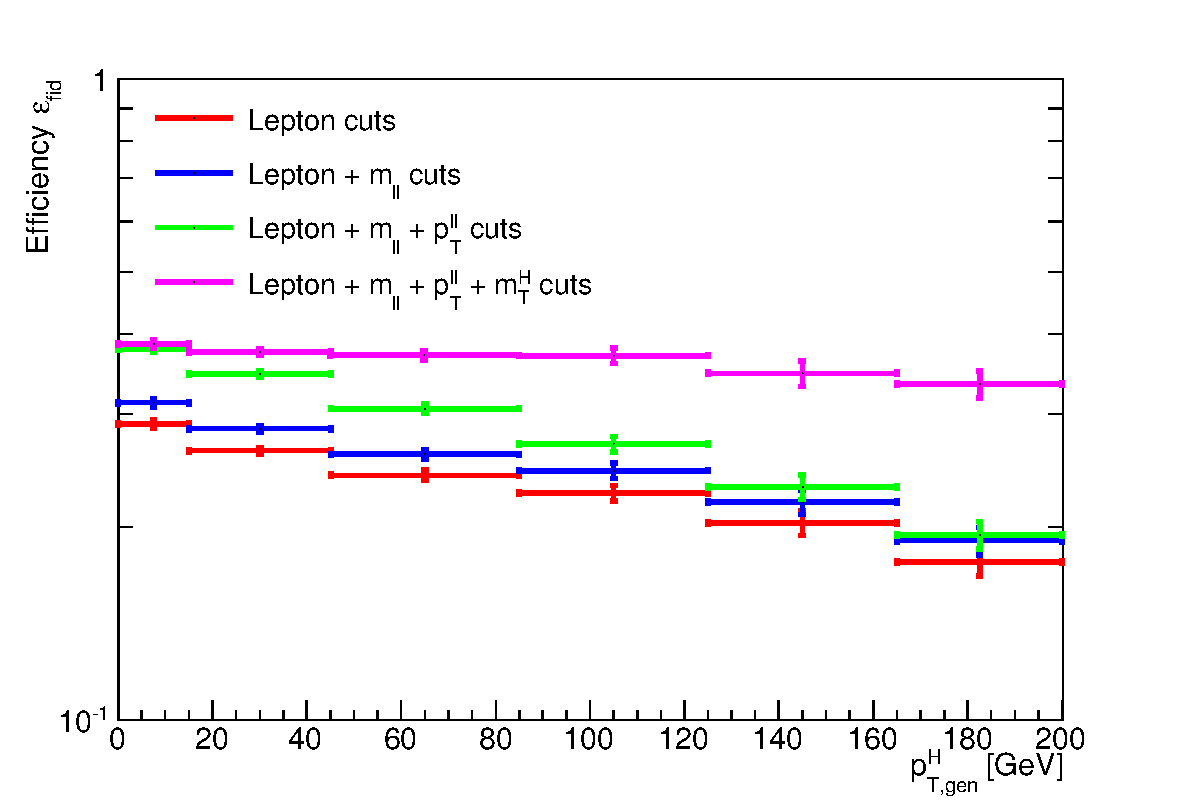
\includegraphics[width=0.45\textwidth]{images/eff-fid.pdf}
}
\subfigure[]{
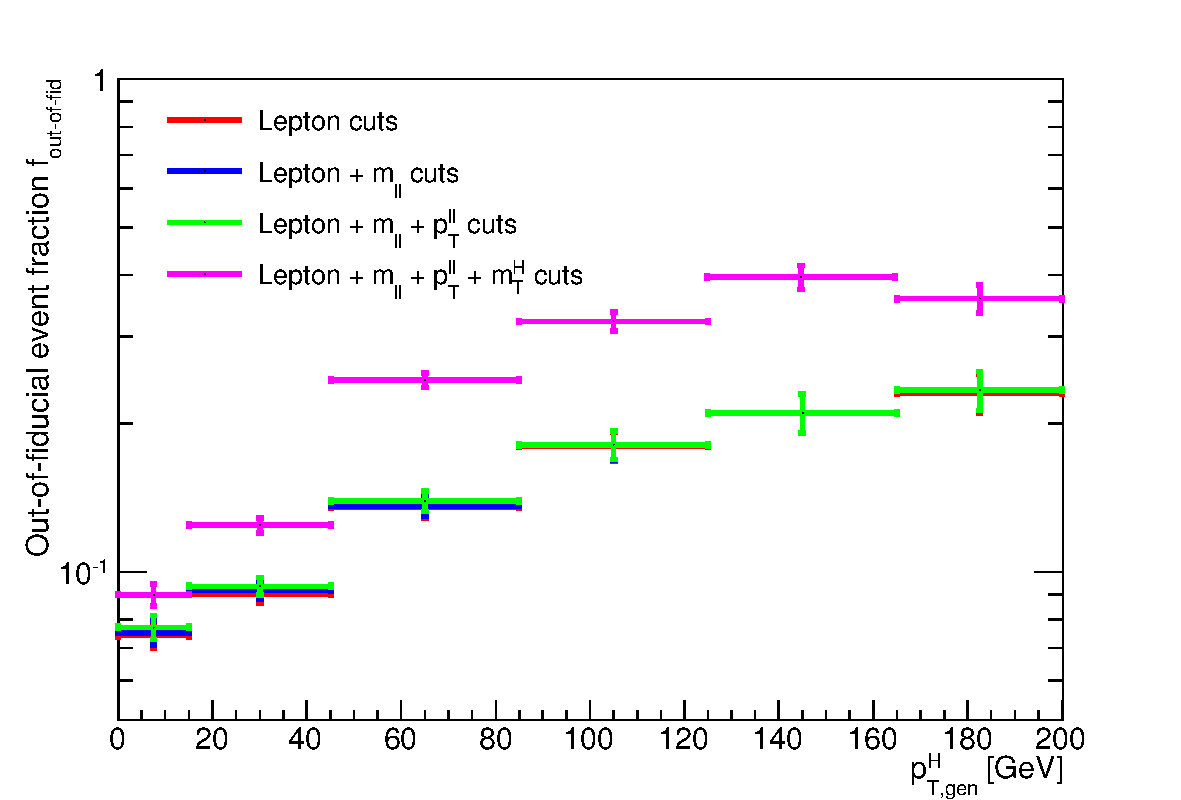
\includegraphics[width=0.45\textwidth]{images/out-of-fid.pdf}
}
\caption{Fiducial signal efficiency $\varepsilon_\mathrm{fid}$ and fraction of out-of-fiducial signal events $f_\mathrm{out-of-fid}$ in each bin of the generator level \pth.\label{fig:sel_eff}}
\end{figure}

If a $4\pi$ acceptance is defined, requiring just that the Higgs decays to WW and then to $2\ell2\nu$, the efficiency becomes $\epsilon=0.0396\pm{0.0003}$ and the fake rate is zero. 






%\clearpage
%-------------------------------------------------------------------------------
\section{Event reconstruction and selections\label{sec:Selections}}

	%--------------------------------------------------------------------------------
	\subsection{Event reconstruction\label{subsec:EventReconstruction}}
The muons, electrons, jets and missing transverse energy (\MET) reconstruction and criteria are described in
in details in~\cite{AN-2012-194}. The following criteria are only a brief summary:
\begin{itemize}
\item {\bf Muons:} {\it GlobalMuon} 
                   (with $\chi^2/ndof < 10$, at least one good muon hit and at least two muon segments in different muon stations)  
                   or {\it TrackerMuon}  (provided it satisfies the "Tracker Muon Last Station Tight" selection). Several cut-based identification 
                   criteria are applied as well as the particle flow (PF) Isolation. In 2012, the PF Isolation is replaced
                   by an MVA algorithm.
\item {\bf Electrons:} {\it GSF Electons}. A MVA identification criteria is applied  as well as an MVA algorithm.
\item {\bf Jets:}  {\it Anti-$k_T$ PF jets} (with R=0.5 and applying L1, L2 and L3 jet energy corrections, including Pile-Up jet corrections from Fastjet method). Only jets and $|\eta|<4.7$ are considered. A specific Pile-Up MVA-based rejection algorithm is applied.   
\item {\bf \MET:}  The \MET is reconstructed the {\it PF Algorithm} or considering {\it only tracks} originating from the same vertex as 
                   the two leptons. In addition, the minimum of the projections of these two \MET to the closest lepton direction if they are in the same hemisphere, otherwise of their original values, is used in the analysis.  
\end{itemize}

	%--------------------------------------------------------------------------------
	\subsection{Event selection\label{subsec:EventSelection}}
Unlike the main \hwwllnn analysis, this analysis is inclusive in number of jets, so we do not have to define different jet multiplicity categories.
The event selection consist of several steps. The first step is to select \WW -like events applying a selection that is heavily based on the main analysis selection except for few different cuts explained below.
The \WW -like event preselection consists of the following set of cuts:
\begin{enumerate}
\item {\bf Lepton preselection}:
  \begin{itemize}
  \item at least two opposite-sign and opposite-flavour ($e\mu$) leptons reconstructed in the event;
  \item $|\eta|<2.5$ for electrons and $|\eta|<2.4$ for muons;
  \item $\pt>20~\GeV$ for the leading lepton. For the trailing lepton, the transverse momentum is required to be larger than 10~\GeV.
  \end{itemize}
\item {\bf Extra lepton veto}: the event is required to have two and only two opposite-sign leptons passing the lepton selection.
\item {\bf \MET preselection}: particle flow \MET is required to be greater than $20$\GeV.
\item {\bf Di-lepton mass cut}: $m_{\ell\ell} > 12$\GeV in order to reject low mass resonances and QCD backgrounds.
\item {\bf Di-lepton $p_T$ cut}: $p_T^{\ell\ell} > 30$\GeV.
\item {\bf projected \MET selection}: minimum projected \MET required to be larger than 20~\GeV.
\item {\bf Transverse mass}: $m_T^H>60$\GeV to reject Drell-Yan to $\tau\tau$ events. 
\end{enumerate}
In addition to the \WW-like preselection other cuts are applied in order to reduce the top background (\ttbar ans single-top), which is one of the main backgrounds in this final state. We operate two different selections depending on the number of jets with $p_T > 30$~\GeV in the event. This is done to suppress the top background both in the low $p_T^H$ region, where 0-jets events have the biggest contribution, and for higher values where also larger jet multiplicity events are important.
The selection for 0-jets events relies on a soft muon veto, which rejects events with non-isolated soft muons (likely belonging to b-jets), and on a soft jets (with $p_T < 30$~\GeV) anti b-tagging requirement.
The latter requirement exploits the Track Counting High Efficiency tagger (TCHE) to reject soft jets that are likely to come from b quarks hadronization.
These are exactly the same requirements applied in the 0-jets bin of the main analysis.

For events with a jet multiplicity greater or equal than one, we apply a different selection with respect to the main analysis. In this case we exploit the good b-tagging performances of the \textit{JetBProbability} tagger to reject all the jets with $p_T > 30$~\GeV that are likely to come from a b quark. This jet veto relies on a cut on the \textit{JetBProbability} tagger discriminant as has been also done in the VH (\hwwllnn) analysis \cite{CMS_PAS_HIG_13-017}. Any jet with a discriminant value below $1.4$ is identified as a non b-jet. The analysis selection requires no b-tagged jets with $p_T > 30$~\GeV.

\begin{figure}[b]
\centering
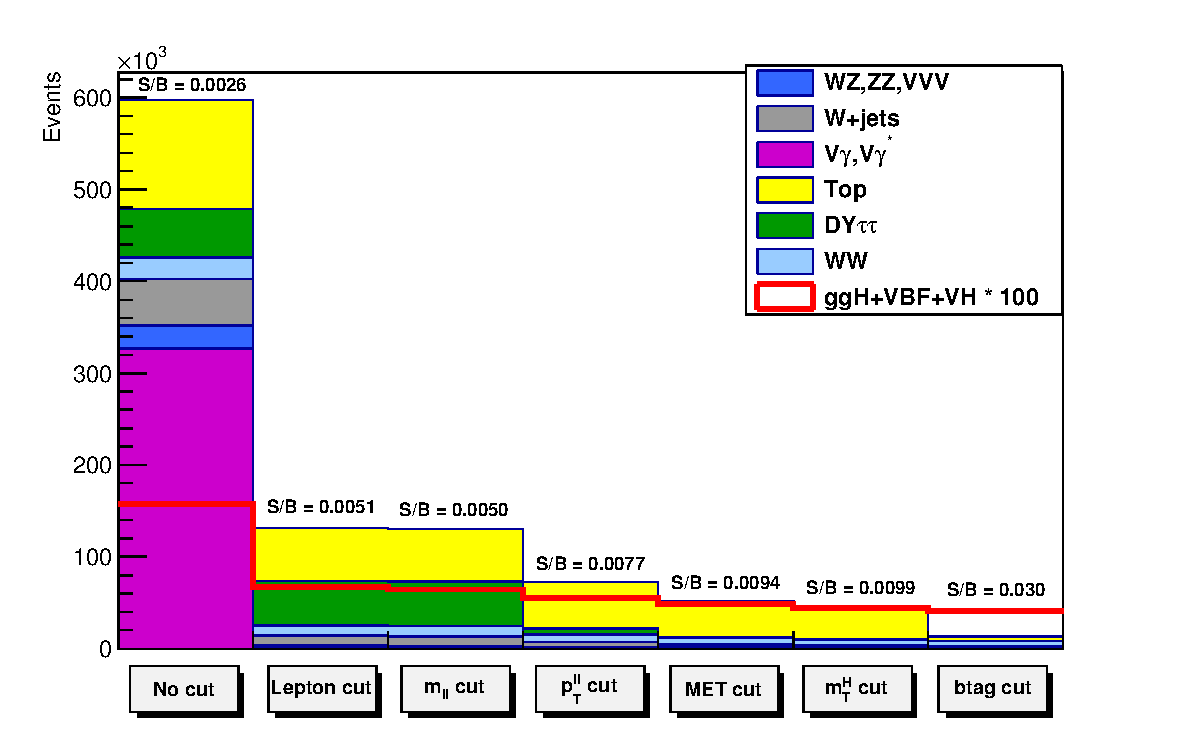
\includegraphics[width=0.8\textwidth]{images/cutflow2.pdf}
\caption{Effect of single selections on MC samples. The signal (red line) is multiplied by 100 and superimposed on stacked backgrounds. In each bin, corresponding to a different selection, is reported the expected number of events in MC at a luminosity of $19.46~\mathrm{fb}^{-1}$.\label{fig:cutflow}}
\end{figure}

A  cut-flow plot is reported in figure \ref{fig:cutflow} showing the effect of each selection on top of Monte Carlo samples. In the first bin, labelled as \textit{No cut}, no selection has been applied and the bin content correspond to the total expected number of events with a luminosity of $19.46~\mathrm{fb}^{-1}$. All the events in this bin have at least two leptons with a loose transverse momentum cut of $8$~\GeV. In the following bin the lepton cuts are applied, including the requirement to have two opposite-sign and opposite-flavour leptons and the extra lepton veto. Then are progressively reported all the other selections, showing the effect of each cut on backgrounds and signal. For each selection is also reported the expected signal over background ratio which after the full selection reach a maximum value around $3\%$.

\begin{figure}[t]
\centering
\subfigure[]{
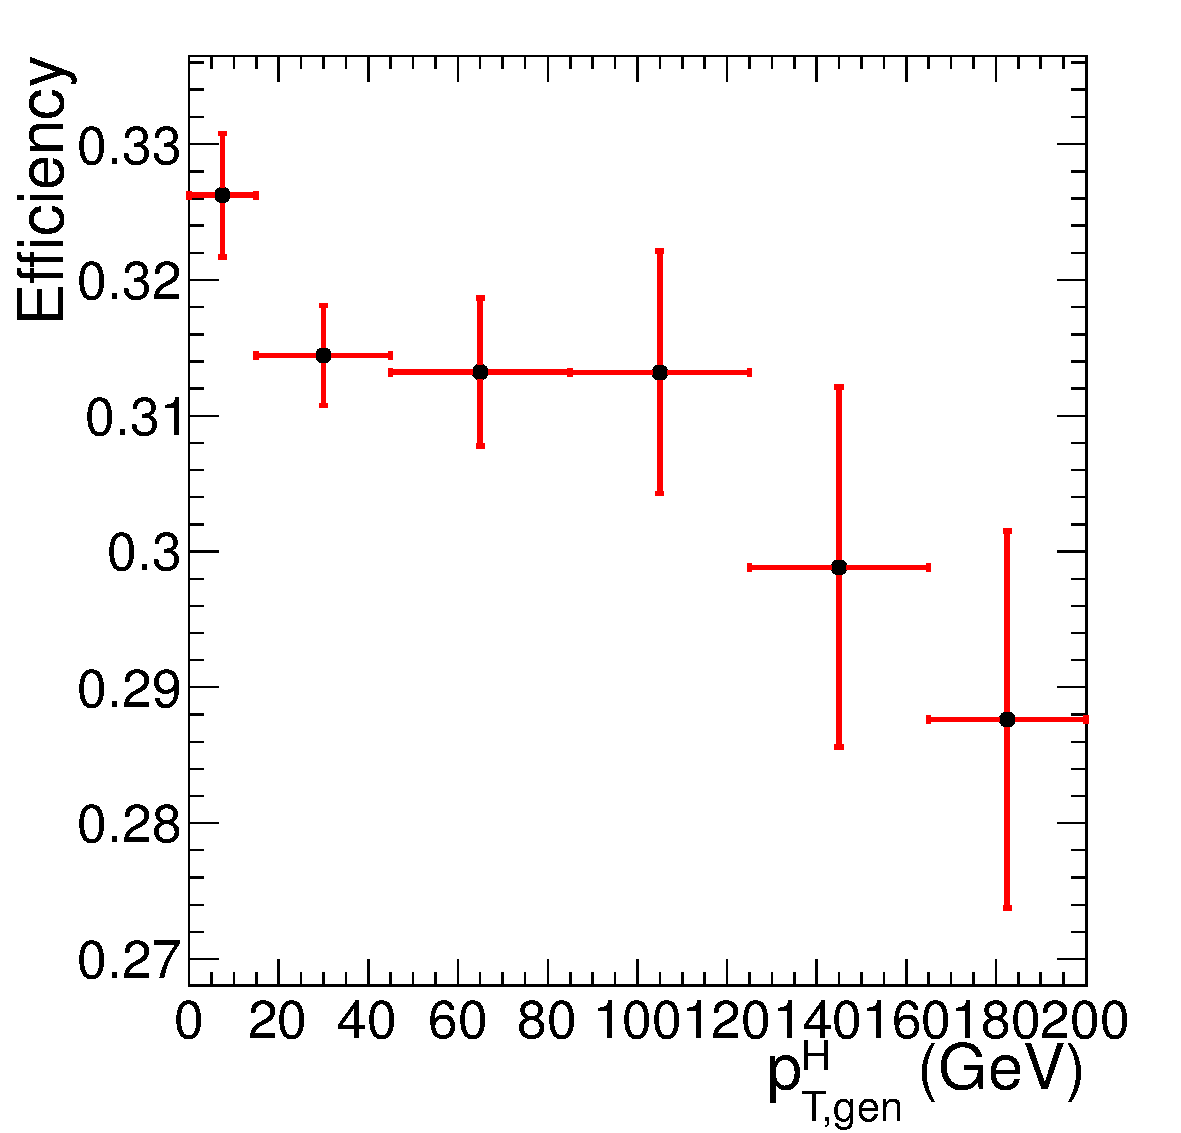
\includegraphics[width=0.4\textwidth]{images/eff_pth.pdf}
}
\subfigure[]{
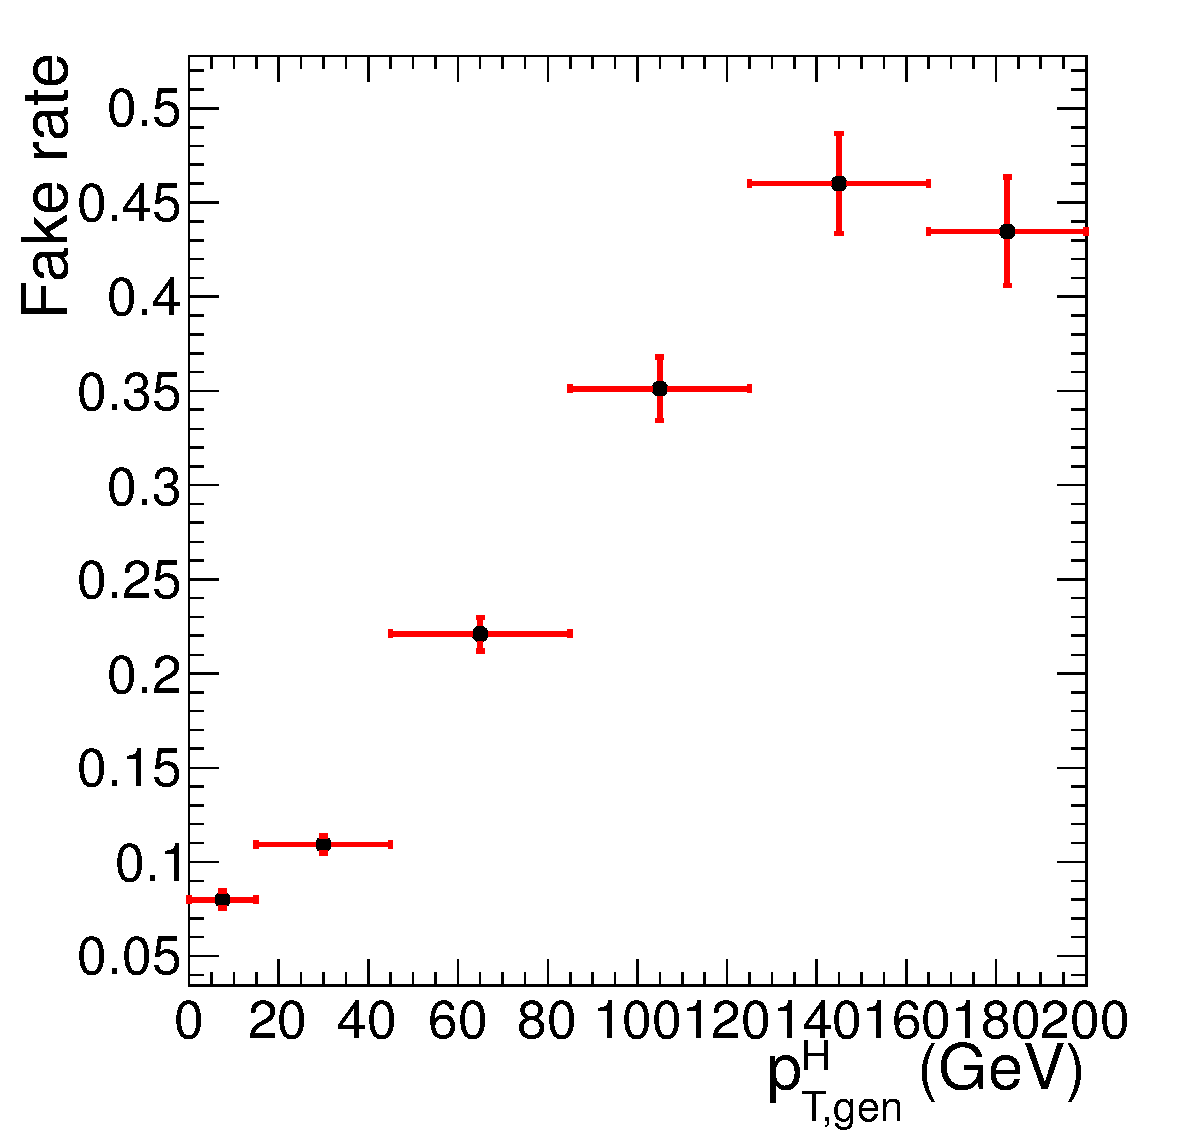
\includegraphics[width=0.4\textwidth]{images/fake_pth.pdf}
}
\caption{Efficiency of the full selection (a) and fake rate (b) as a function of $p_T^H$.\label{fig:sel_eff}}
\end{figure}

The selection efficiency is shown in Fig.~\ref{fig:sel_eff} (a). The efficiency denominator is the number of events that pass the acceptance, while the numerator is the number of events that pass both the selection and the acceptance, in each \pth bin. The fake rate, defined by the ratio of signal events that pass the selection but are not within the acceptance, divided by the total number of events passing both the selection and the acceptance is shown in Fig.~\ref{fig:sel_eff} (b). For both the selection efficiency and the fake rate the signal samples included correspond to the \textit{ggH}, \textit{VBF} and \textit{VH} production mechanisms.
The overall efficiency and fake rate are: $\epsilon=0.362\pm{0.005}$ and $fake~rate=0.126\pm0.004$, where the errors are only statistical.

If we define a $4\pi$ acceptance, requiring just that the Higgs decays to WW and then to $2l2\nu$, the efficiency is $\epsilon=0.03960\pm{0.00033}$. 


%\clearpage
\section{Binning of the \pth spectrum}
%%%%%%%%%%%%%%%%%%%%%%%%%%%%%%%%%%%%%%%%%%%%%%%%%%%%%%%%%%%%%%%%%%%%%%
\label{sec:Binning}

Given the limited resolution on $\pth$, a criterion is needed to establish bi size. The criterion that we have chose is devised to keep under control the bin migrations due to the finite resolution. 
For any given bin $i$ we can define the purity $P_i$ on a signal sample as the number events that are generated and also reconstructed in that bin, $N_i^{GEN|RECO}$, divided by the number of events reconstructed there $N_i^{RECO}$:
\begin{equation}
P_i = \frac{N_i^{GEN|RECO}}{N_i^{RECO}} \qquad .
\end{equation}
Where $N_i^{GEN|RECO}$ is the number of events that are both generated and
reconstructed in a $\pth$ bin $i$, while $N_i^{RECO}$ is the number of events
that are reconstructed in bin $i$. We have chosen the bin width in such a way
as to make the smallest bins able to ensure a purity of about 60\% on a gluon fusion sample.
Following this prescription we have divided the whole $\pth$ range in six
different bins: \mbox{[0-15 GeV]}, \mbox{[15-45 GeV]}, \mbox{[45-85 GeV]},
\mbox{[85-125 GeV]}, \mbox{[125-165 GeV]}, \mbox{[165-$\infty$ GeV]}.
%Mettere plot binning
A two-dimensional histogram  has been made putting the GEN level $\pth$ on the x-axis (calculated using the WW system transverse momentum) and the RECO one on the y-axis. Each row is then normalized to one in order to directly have the purity in the diagonal bins. Also the effect of bin migration due to finite detector resolution effects can be assessed from this plot.\\
This two dimensional plot is shown in Fig.~\ref{fig:response_by_row} (a) and (b) for gluon fusion and VBF signals for $m_\mathrm{H}=125$\GeV.
\begin{figure}[b]
\centering
\subfigure[ggH]{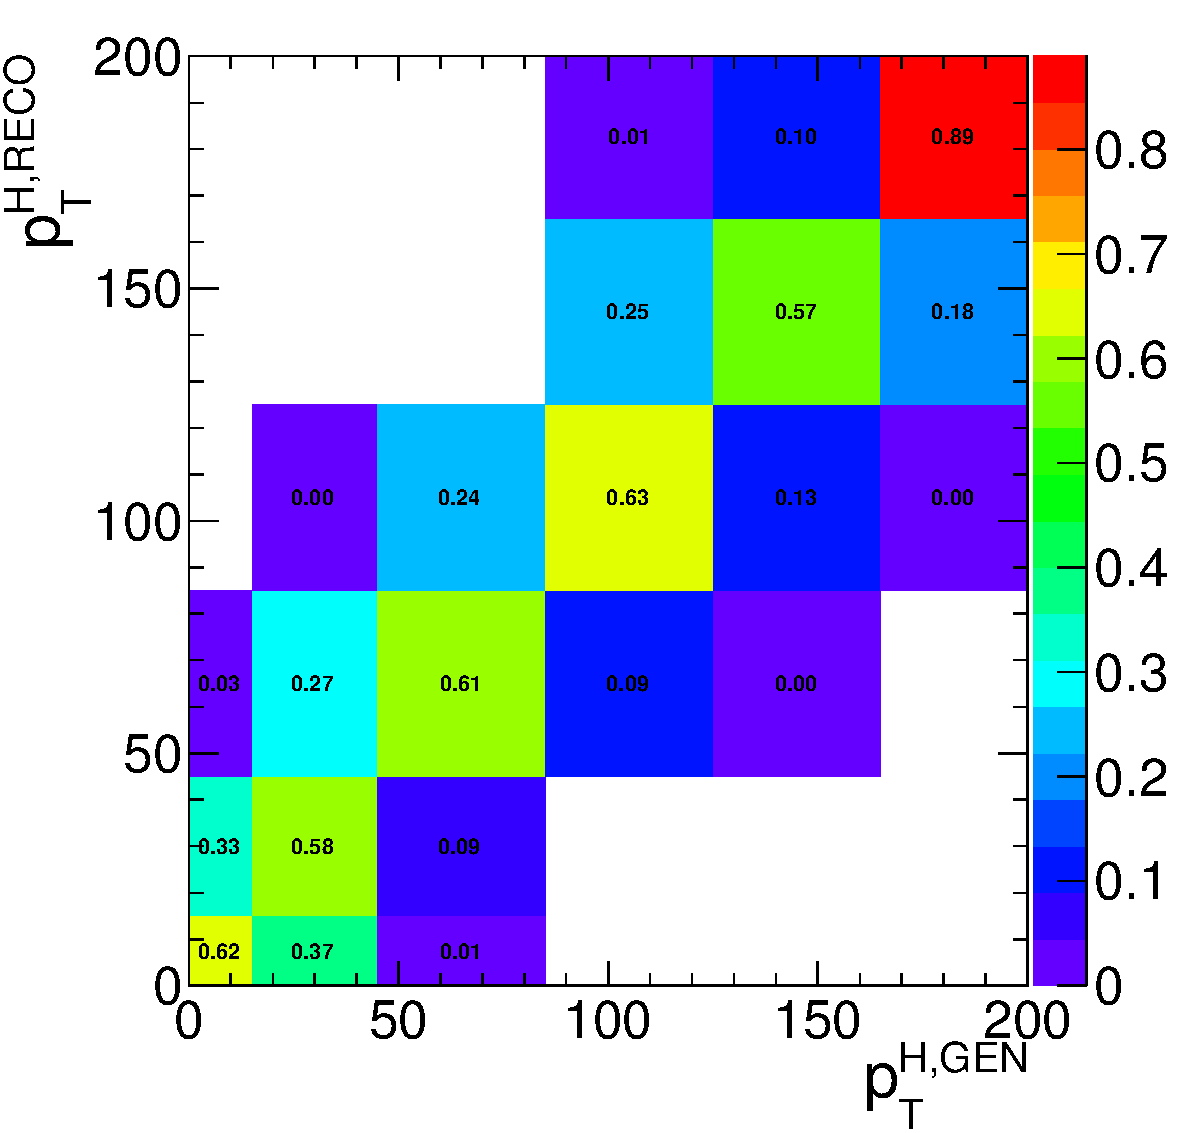
\includegraphics[width=0.45\textwidth]{images/response_ggH_norm_by_row.pdf}}
\subfigure[qqH]{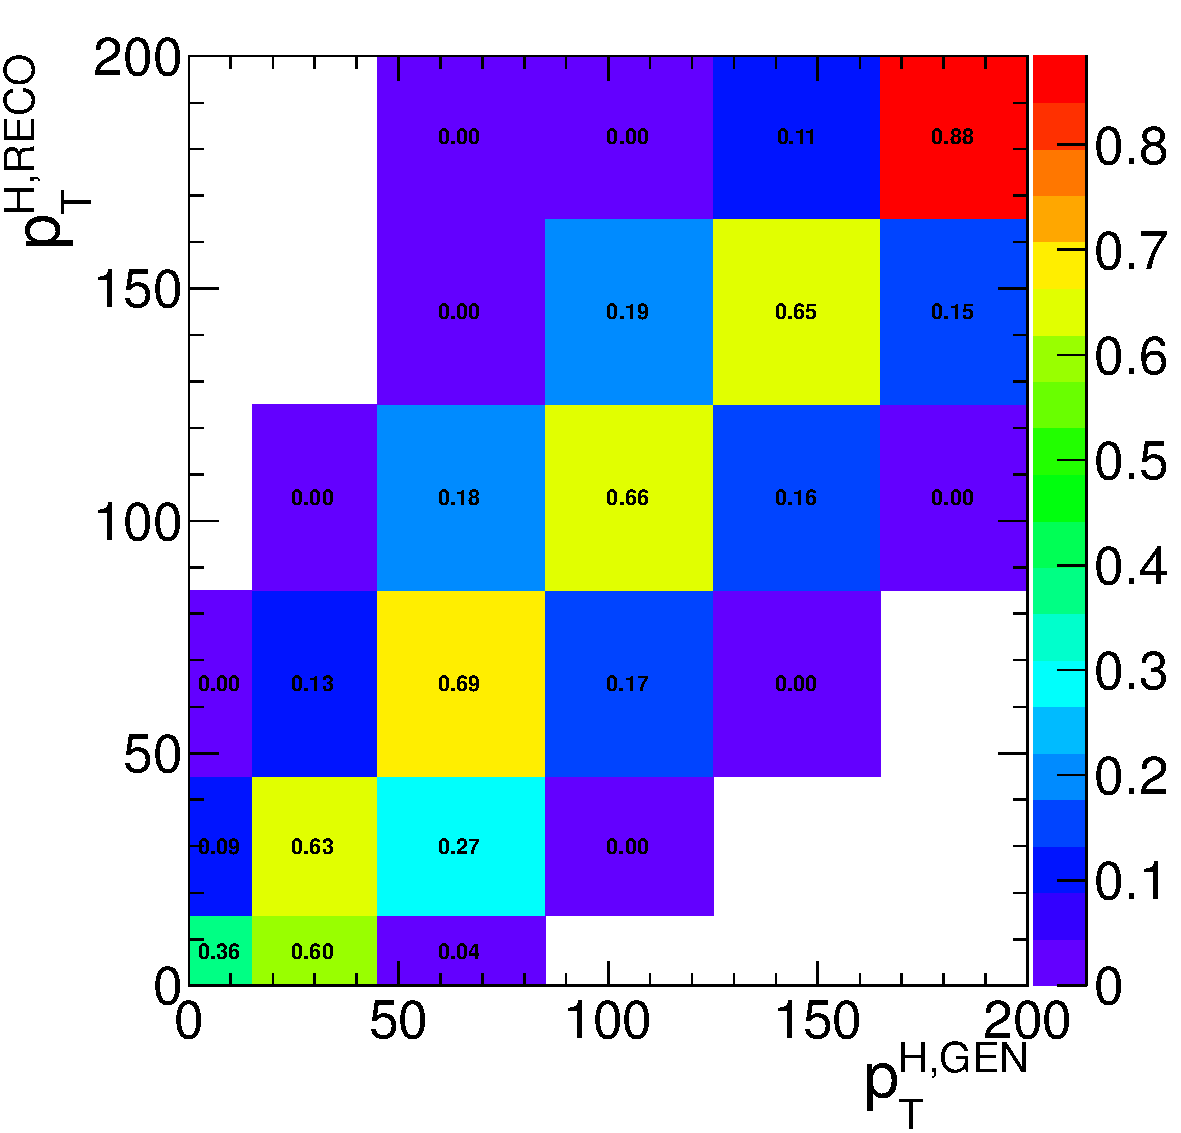
\includegraphics[width=0.45\textwidth]{images/response_qqH_norm_by_row.pdf}}
\caption{Reconstructed versus generated $\pth$ for gluon fusion (a) and VBF (b). Plots are normalized by rows, so that the bin purity is shown on the diagonal.\label{fig:response_by_row}}
\end{figure}

%\clearpage
\section{Background estimation}
%%%%%%%%%%%%%%%%%%%%%%%%%%%%%%%%%%%%%%%%%%%%%%%%%%%%%%%%%%%%%%%%%%%%%%
\label{sec:Backgrounds}

\textcolor{red}{Add plots for each background process}

\subsection{Top quark background \label{sec:TTBackground}}

In this analysis the top quark background is divided into two different categories depending on the number of jets in the event. In the two categories different selections are applied, especially concerning the b-tagging requirements.

The general strategy for determining the residual top events in the signal region is to first measure the top tagging efficiencies from an orthogonal region of phase space in data. The orthogonal phase space is  defined inverting the b-veto requirement of the signal region, in such a way to have a control region enriched in top quark events.  Then, using this efficiency, the number of events with the associated uncertainty is propagated from the control region to the signal region.
The number of surviving top events in the signal region would then be:

\begin{equation}
 N^{\mathrm{signal}}_{bveto} = N^{\mathrm{control}}_{btag} \cdot \frac{1-\epsilon_{\mathrm{top}}}{\epsilon_{\mathrm{top}}}
\label{eq:top_equation}
\end{equation}

where $N^{\rm control}_{\rm btag}$ is the number of events in the 
control region and $\epsilon_{\rm top}$ is the efficiency as measured
in data.

The methods to estimate the top background contribution in the two jet categories are different and are explained below.


\subsubsection{0-jets category}
Most of the top background, composed of \ttbar and tW processes, is rejected in the 0-jet bin by the
jet veto. The top-tagging efficiency in the zero jet bin, $\epsilon_{\rm tag}^{0-jet}$, is the probability for a top event to
fail one of either the b-tagging veto or the soft muon veto, and is defined as:

\begin{equation}\label{eq:eff_top_0j}
\epsilon_{\rm tag} = \frac{N_{\rm tag}^{\rm control}}{N^{\rm control}} \quad ,
\end{equation}

where $N^{\rm control}$ is the number of events in the top control phase space defined requiring one b-tagged jet with $\pt>30$\GeV, and $N_{\rm tag}^{\rm control}$ is the subset of those events that pass either the soft muon tagging or the low-\pt b jet tagging. The purity of this control sample, as estimated from simulation, is about 97\%. The remaining 3\% background contribution is estimated from simulation and subtracted from the numerator and denominator of Eq.~\eqref{eq:eff_top_0j}. The efficiency $\epsilon_{\rm top}^{0-jet}$ can then be estimated using the following formula:

\begin{equation}\label{eq:eff_top_0j}
\epsilon_{\rm top}^{0-jet} = f_{\ttbar} \cdot \epsilon_{2b} + f_{tW} \cdot ( x \cdot \epsilon_{2b} + (1-x) \cdot \epsilon_{\rm tag} ) \quad ,
\end{equation}

\begin{equation}
\epsilon_{2b} = 1 - (1 - \epsilon_{\rm tag})^{2} \quad ,
\end{equation}
where $f_{\ttbar}$ and $f_{tW}$ are the \ttbar and tW fractions respectively, $x$ is the fraction of tW events containing 2 b jets, and $\epsilon_{2b}$ is the efficiency for a top event with 0 counted jets, i.e. two soft b jets, to pass the top veto. For the ratio of \ttbar and tW cross-sections an uncertainty of 17\% is assumed. The fraction $f_{\ttbar}$ is estimated using MC simulation of the \ttbar and tW processes at NLO accuracy.

Using this procedure a data/simulation scale factor of $0.98 \pm 0.17$ is found, and is applied to correct the MC simulation in order to match the data.



\subsubsection{Category with more than 0 jets}
The strategy for the estimation of the top background in events with at least one jet with $\pt$ greater than 30 \GeV is the following. First of all the efficiency for tagging a b jet is measured both in data and simulation and the values are used to correct the simulation for different b-tagging efficiencies in data and simulation. This evaluation is performed in a control region, called CtrlTP, containing at least two jets, using a Tag\&Probe technique. The procedure to extract these scale factors is presented in Sec.~\ref{sec:TagAndProbe}. Then a larger statistics control region, CtrlDD, is defined by requiring at least one b-tagged jet and we use the simulation, corrected for the previously computed b-tagging efficiency scale factor, to derive the factor that connects the number of events in CtrlDD to the number of events in the signal region. This second step is explained in detail in Sec.~\ref{sec:DD}. 

\subsubsection{Tag\&Probe \label{sec:TagAndProbe}}
The Tag\&Probe technique is a method to estimate the efficiency of a selection on data. In can be applied whenever one has two objects in one event, by using one of the two, the \tg{}, to identify the process of interest, and using the second, the \probe{}, to actually measure the efficiency of the selection being studied. In our case we want to measure the b-tagging efficiency, so what we need is a sample with two b-jets per event. The easiest way to construct such a sample is to select $t\bar{t}$ events.

The CrtlTP control region is defined selecting the events which pass the lepton preselection cuts listed in Sec.~\ref{subsec:EventSelection}, and have at least two jets with \pt greater than 30 \GeV.
One of the two leading jets is required to have a \jpb score higher than 0.5. From events in this control region we built \tp{} pairs as follows. For each event the two leading jets are considered. If the leading jet passes the \jpb cut of 0.5, that is considered a \tg{}, and the sub-leading jet is the \probe{}. In order to avoid any bias that could arise from the probe being always the second jet, the pair is tested also in reverse order, meaning that the sub-leading jet is tested against the \tg{} selection, and in case it passes, then the leading jet is used as \probe{} in an independent \tp{} pair. This means that from each event passing the CrtlTP cuts one can build up to two \tp{} pairs. 

If the \tg{} selection were sufficient to suppress any non top events, one could estimate the efficiency by dividing the number of \tp{} pairs in which the \probe{} passes the analysis cut \jpb$>$1.4 (\tpp) by the total number of \tp{} pairs. However this is not the case. 
In order to estimate the efficiency in the presence of background a variable that discriminates between true b-jets and other jets in a $t\bar{t}$ sample is chosen. The variable is the \pt of the \probe{} jet. For real b-jets this variable has a peak around 60 \GeV, while it does not peak for other jets. The idea is to fit simultaneously the \pt spectrum for \probe{} jets in \tpp{} and \tfp{} pairs, linking together the normalizations of the two samples as follows:
\begin{equation}
N_{TPP}=N_{s}\epsilon_{s} + N_b\epsilon_{b}
\end{equation}
\begin{equation}
N_{TFP}=N_{s}(1-\epsilon_{s}) + N_b(1-\epsilon_{b})
\end{equation}
where $N_{\rm TPP}$ is the number of \tpp{} pairs, $N_{\rm TFP}$ is the number of \tfp{} pairs, $N_{\rm s}$ is the number of \tp{} pairs in which the probe is a b-jet, $N_{\rm b}$ is the number of \tp{} pairs in which the probe is a not b-jet, $\epsilon_{\rm s}$ is the b-tagging efficiency, $\epsilon_{\rm b}$ is the probability of identifying as b-jet a non-b-jets, i.e. the mistag rate. 

A $\chi^{2}$ simultaneous fit of the \probe{} \pt spectrum for \tpp{} and \tfp{} pairs is performed, deriving the shapes for true b-jets and non-b-jets from the simulation, and extracting $N_{\rm s}$, $N_{\rm b}$, $\epsilon_{\rm s}$ and $\epsilon_{\rm b}$ from the fit.
The result of the fit on simulation is shown in Fig.~\ref{fig:mc_tp}. The relevant efficiencies are:
\begin{equation}
\epsilon_{s}^{MC}=0.7663\pm0.0072
\end{equation}
\begin{equation}
\epsilon_{b}^{MC}=0.208\pm0.015
\end{equation}
We have checked that these values are consistent with the true value for the b-tagging efficiency. The true value is computed by selecting jets that are matched within a cone of $\Delta{R}<0.5$ with a generator level b-quark, and counting the faction of those that pass the \jpb cut of 1.4. This means that the \tp{} method does not introduce biases within the simulation statistic accuracy.

\begin{figure}[b]
\centering
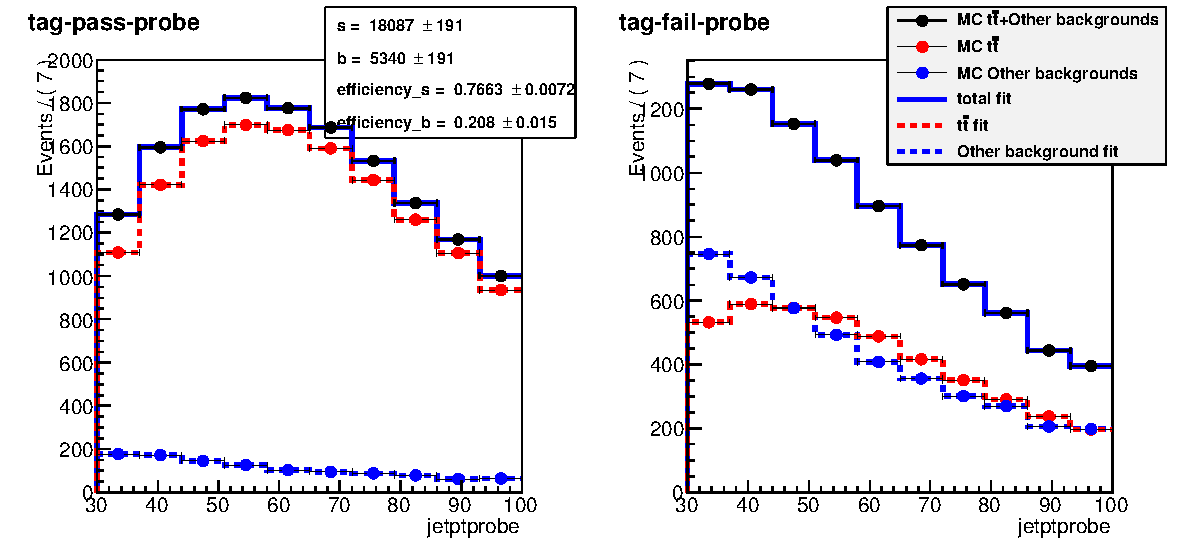
\includegraphics[width=0.8\textwidth]{images/mc_pt_probe.pdf}
\caption{Simultaneous fit of the \tpp{} and \tfp{} pairs in the MC.\label{fig:mc_tp}}
\end{figure}

In order to assess the robustness of the fit, 5000 toy MC samples have been generated with a statistics equivalent to the one expected in data and the same fit is performed. All the 5000 fit succeeded, and the pull distributions for $\epsilon_{\rm s}$ and $\epsilon_{\rm b}$ parameters are shown in Fig.~\ref{fig:pullstp}. The plots show the pull of the efficiencies measured in the fit, where the pull variable for each toy $i$ is defined as:

\begin{equation}
pull(\epsilon_{\rm s (b)}) = \frac{\epsilon_{\rm s (b)}^{\rm true} - \epsilon_{\rm s (b)}^{i}}{\sigma(\epsilon_{\rm s (b)}^{i})}
\end{equation}

The pulls are centered on 0 and have $\sigma$ close to 1, as expected.

\begin{figure}[t]
\centering
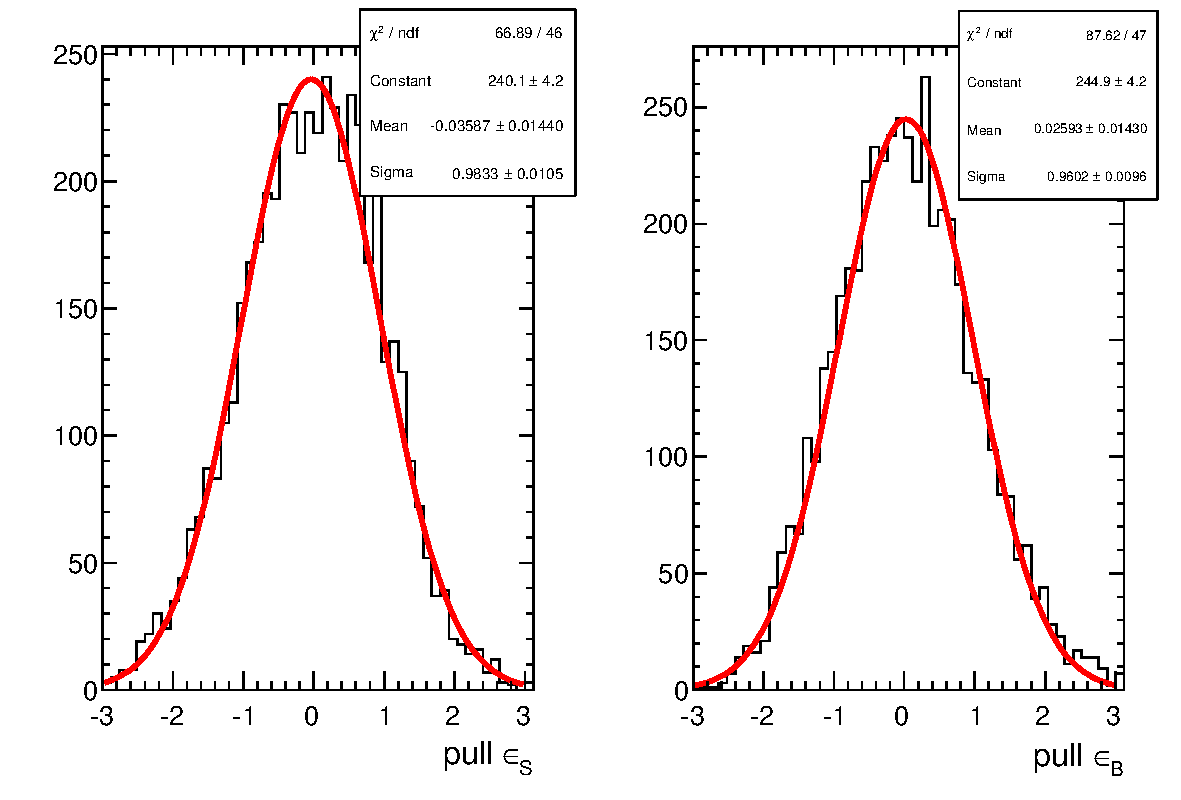
\includegraphics[width=0.8\textwidth]{images/pulls_mc.pdf}
\caption{Pulls of the $\epsilon_{s}$ and $\epsilon_{b}$ parameters in 5000 toy MC.\label{fig:pullstp}}
\end{figure}
An example fit for one of the toys is shown in  Fig.~\ref{fig:toy_tp}
\begin{figure}[b]
\centering
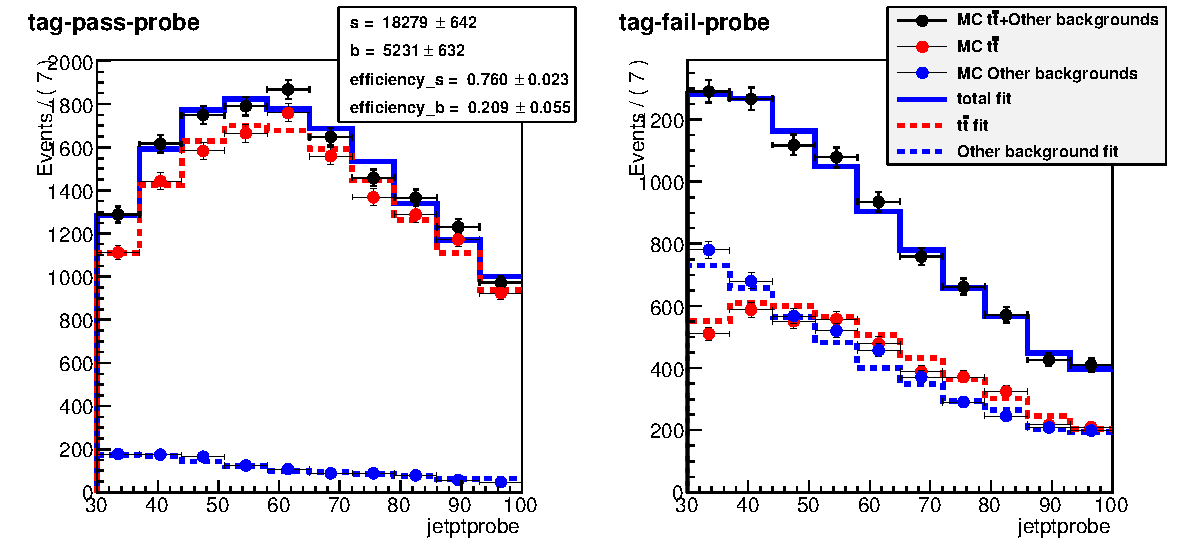
\includegraphics[width=0.8\textwidth]{images/mc_pt_probe_toy.pdf}
\caption{Fit of a toy MC sample.\label{fig:toy_tp}}
\end{figure}

Before running the fit on data, the shapes used in the fit have been validated. To do so, a purer top enriched phase space has been defined by requiring exactly two jets with \jpb score higher than 1.5 and no additional b-tagged jets, rejecting also jets with \pt smaller than 30 \GeV. On this purer sample we have compared data against the shape used to fit the true b-jets in the \tpp{} distribution. The result is shown in Fig.~\ref{fig:purett} and shows good agreement.
\begin{figure}[t]
\centering
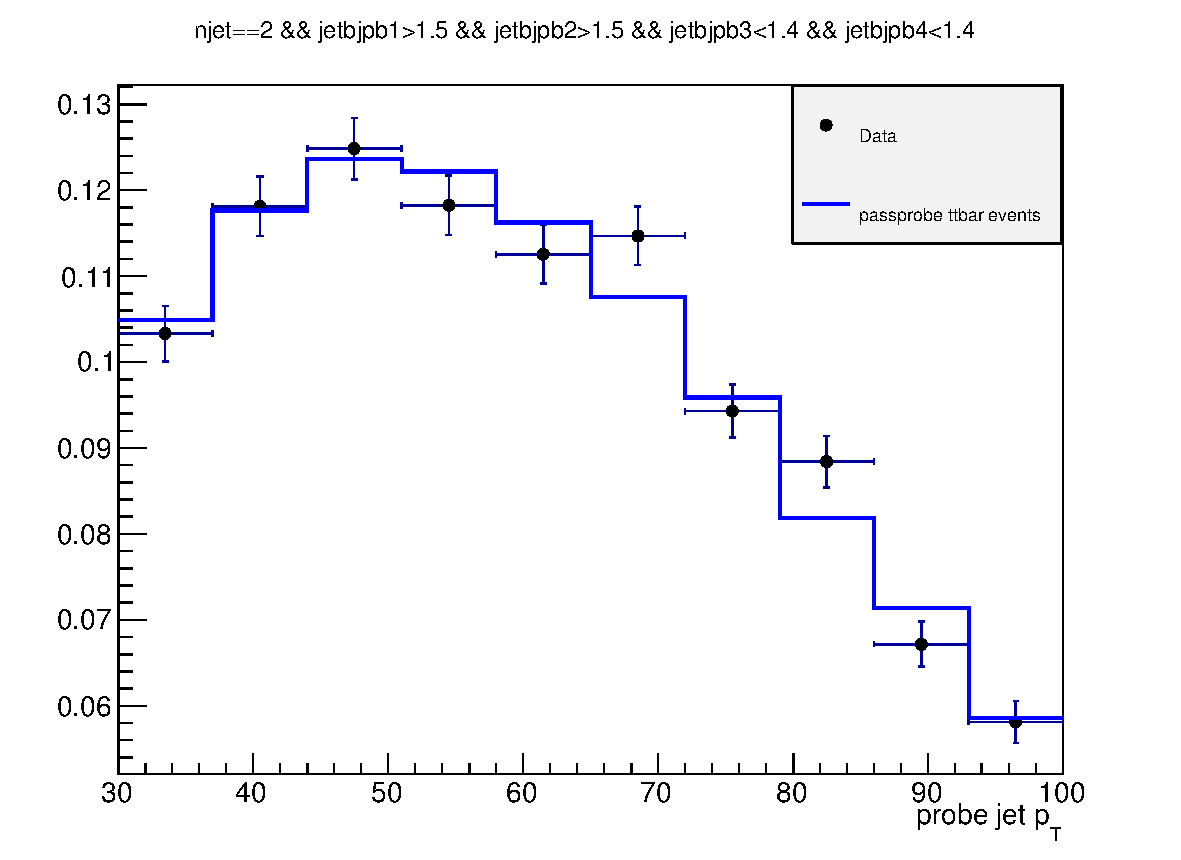
\includegraphics[width=0.6\textwidth]{images/passprobe_data_mc.pdf}
\caption{Shape comparison for the \probe{} \pt spectrum in data and in MC in a very pure \ttbar sample.\label{fig:purett}}
\end{figure}

Finally the fit has been performed on data, as shown in Fig.~\ref{fig:data_tp}, providing the following efficiencies:
\begin{equation}
\epsilon_{s}^{Data}=0.769\pm0.022
\end{equation}
\begin{equation}
\epsilon_{b}^{Data}=0.121\pm0.054
\end{equation}

\begin{figure}[b]
\centering
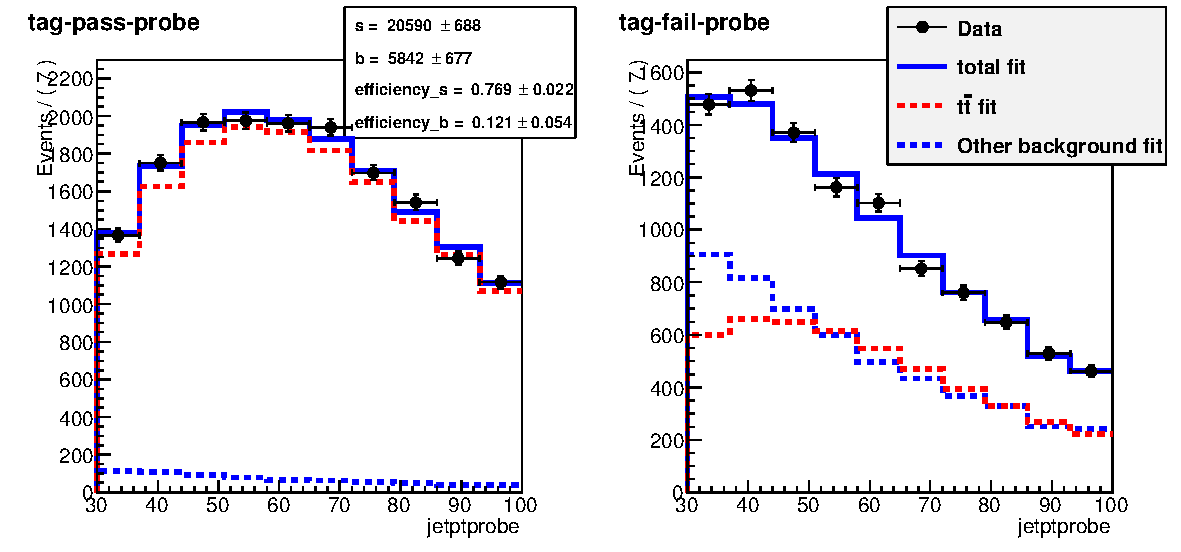
\includegraphics[width=0.8\textwidth]{images/data_ptprobe.pdf}
\caption{Simultaneous fit of the \tpp{} and \tfp{} pairs in data.\label{fig:data_tp}}
\end{figure}

Further studies have been performed to assess the effect of the relative uncertainty on the \ttbar and tW event fractions. The same procedure described above has been applied to different simulation templates obtained varying the \ttbar and tW fractions within theoretical uncertainties, and the effect on the parameters extracted with the fit procedure is found to be well below the fit uncertainties.


\subsubsection{Data driven estimation \label{sec:DD}}
In addition to the b-tagging efficiency, the other ingredient to estimate the \ttbar background is the process cross section. The idea is to measure the cross section in a \ttbar enriched control region, that is called CtrlDD. CtrlDD is defined according to the lepton preselection cuts defined in Sec.~\ref{sec:Selections}, and requiring in addition at least one jet with \jpb score higher than 1.4.

From the simulation we derive the factor $\alpha$ that connects CrtlDD to the signal region, calculating the ratio of \ttbar events in the two regions:

\begin{equation}
\alpha=\frac{N_{\ttbar~MC}^{SIG}}{N_{\ttbar~MC}^{CtrlDD}} \quad.
\end{equation}

The number of events in the CtrlDD region in data is counted, subtracting the expected number of events from non-\ttbar backgrounds, and obtaining $N_{\ttbar~Data}^{CtrlDD}$. Finally the number of expected \ttbar events in the signal region ($N_{\ttbar~Data}^{SIG}$) is obtained as:

\begin{equation}
N_{\ttbar~Data}^{SIG} = \alpha{}N_{\ttbar~Data}^{CtrlDD}.
\end{equation}

In evaluating $\alpha$ and its error the b-tagging efficiencies determined in Sec.~\ref{sec:TagAndProbe} are used. 
For each event an efficiency scale factor and a mistag rate scale factor are derived, depending on whether the event falls in the signal or CtrlDD region.

\begin{equation}
\label{eq:sfsig}
SF_{SIG} = \left(\frac{1-\epsilon_{s}^{Data}}{1-\epsilon_{s}^{MC}}\right)^{min(2, n_{b-jets})} \left(\frac{1-\epsilon_{b}^{Data}}{1-\epsilon_{b}^{MC}}\right)^{n_{non-b-jets}} 
\end{equation}

\begin{equation}
\label{eq:sfbkg}
SF_{CtrlDD} = \left(\frac{\epsilon_{s}^{Data}}{\epsilon_{s}^{MC}}\right)^{(jet1 == b-jet)} \left(\frac{\epsilon_{b}^{Data}}{\epsilon_{b}^{MC}}\right)^{(jet1 == non-b-jets)} 
\end{equation}

where $n_{b-jets}$ is the number of true b-jets in the event and $n_{non-b-jets}$ is the number of non-b-jets in the event. The writing $jet1 == b-jet$ ($jet1 == non-b-jets$) is a boolean flag that is true when the leading jet, the one used for the CtrlDD selection, is (not) a true b-jet.

Since the efficiency and mistag rate that have been measured on data are close to the one in the simulation, it was decided to assume a scale factor of 1 for both b-tagging efficiency and mis-tag rate. This means that the central values of the scale factors defined in Eq.~\ref{eq:sfsig} and Eq.~\ref{eq:sfbkg} is 1, but these numbers have an error that is derived assuming an uncertainty on $\epsilon_{s}^{Data}$ and $\epsilon_{b}^{Data}$ that covers both the statistical error from the fit of the two quantities and the difference with respect to the simulation.
This results in an up and a down variation of the scale factors in the signal and CtrlDD regions, that is used to derive an error on $\alpha$.

A data driven estimation of the top quark background with the method described above is performed in each of the \pth bins independently. The reason to make this estimation in $\pth$ bins, rather than inclusively is explained in Fig.~\ref{fig:ttpth}, where the \pth distribution is shown in the CtrlDD region normalized to the cross section measured by a specific CMS analysis~\cite{Khachatryan:2016mqs}. As shown in the ratio plot, an overall normalization factor would not be able to accommodate for the variations of the data/simulation ratio from bin to bin.

\begin{figure}[b]
\centering
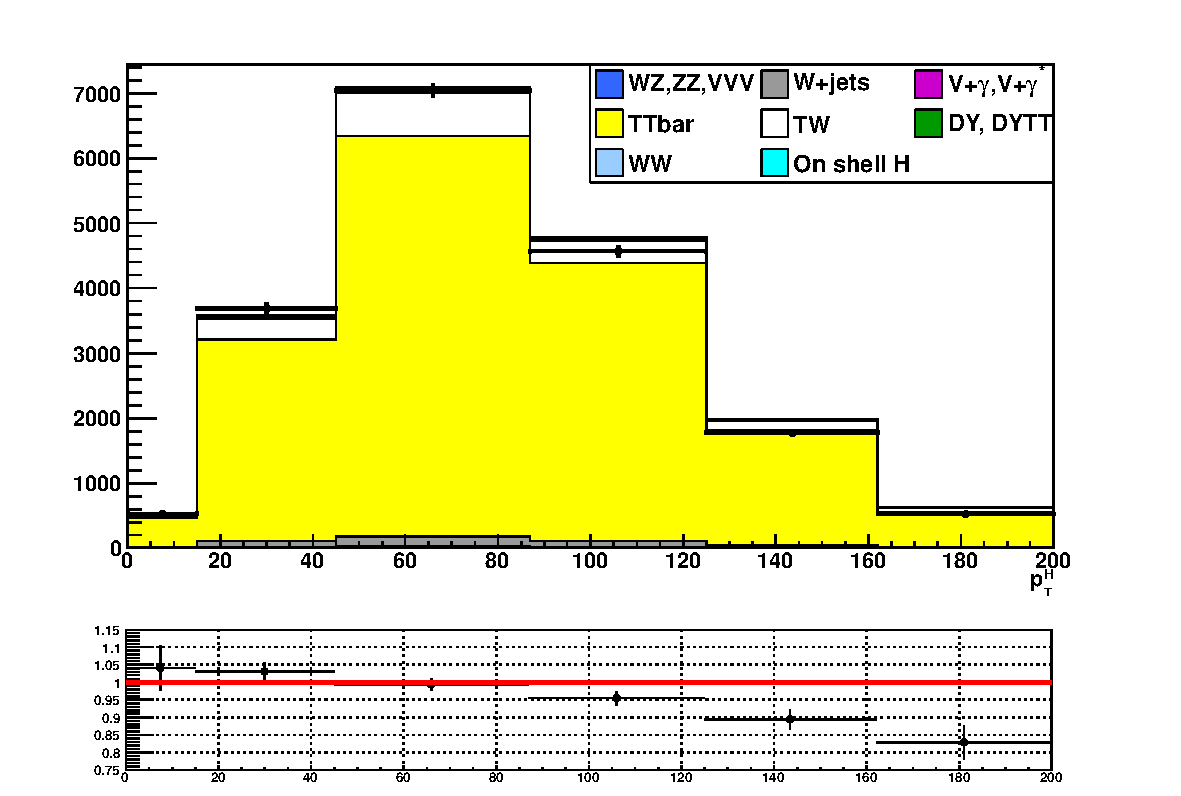
\includegraphics[width=0.6\textwidth]{images/ttpth.pdf}
\caption{$\pth$ distribution in the CtrlDD control region.\label{fig:ttpth}}
\end{figure}

The $\alpha$ factors for each bin and the number of events in signal, CtrlDD regions in MC as well as in data are listed in Tab.~\ref{tab:ttdd}.
\begin{table}
\centering
\begin{tabular}{c c c c c c}
\hline
\pth [\GeV] & $N_{CTRL}^{DATA}$ & $N_{CTRL}^{TOP}$ &  $N_{SIG}^{TOP}$ &
$\alpha$ & $\Delta\alpha$ \\ 
\hline\hline
$[0--15]$ & 406.71 & 358.78 & 117.83 & 0.328 & 0.075 \\ 
$[15--45]$ & 2930.14 & 2703.44 & 859.08 & 0.318 & 0.071 \\ 
$[45--85]$ & 5481.02 & 5207.48 & 1506.05 & 0.289 & 0.065 \\ 
$[85--125]$ & 4126.35 & 4032.56 & 861.22 & 0.214 & 0.052 \\ 
$[125--165]$ & 1612.64 & 1654.27 & 304.69 & 0.184 & 0.055 \\ 
$[165--\infty]$ & 647.50 & 760.37 & 201.70 & 0.265 & 0.147 \\ 
\hline
\end{tabular}
\caption{Data driven scale factors related to the top quark background estimation.\label{tab:ttdd}}
\end{table}

A comparison of the $\mll$ distribution in the six $\pth$ bins used in the analysis in CtrlDD after the data driven correction is shown in Fig.~\ref{fig:mllCtrlDD}
\begin{figure}[htb]
\centering
\subfigure[$\pth<15\GeV$]{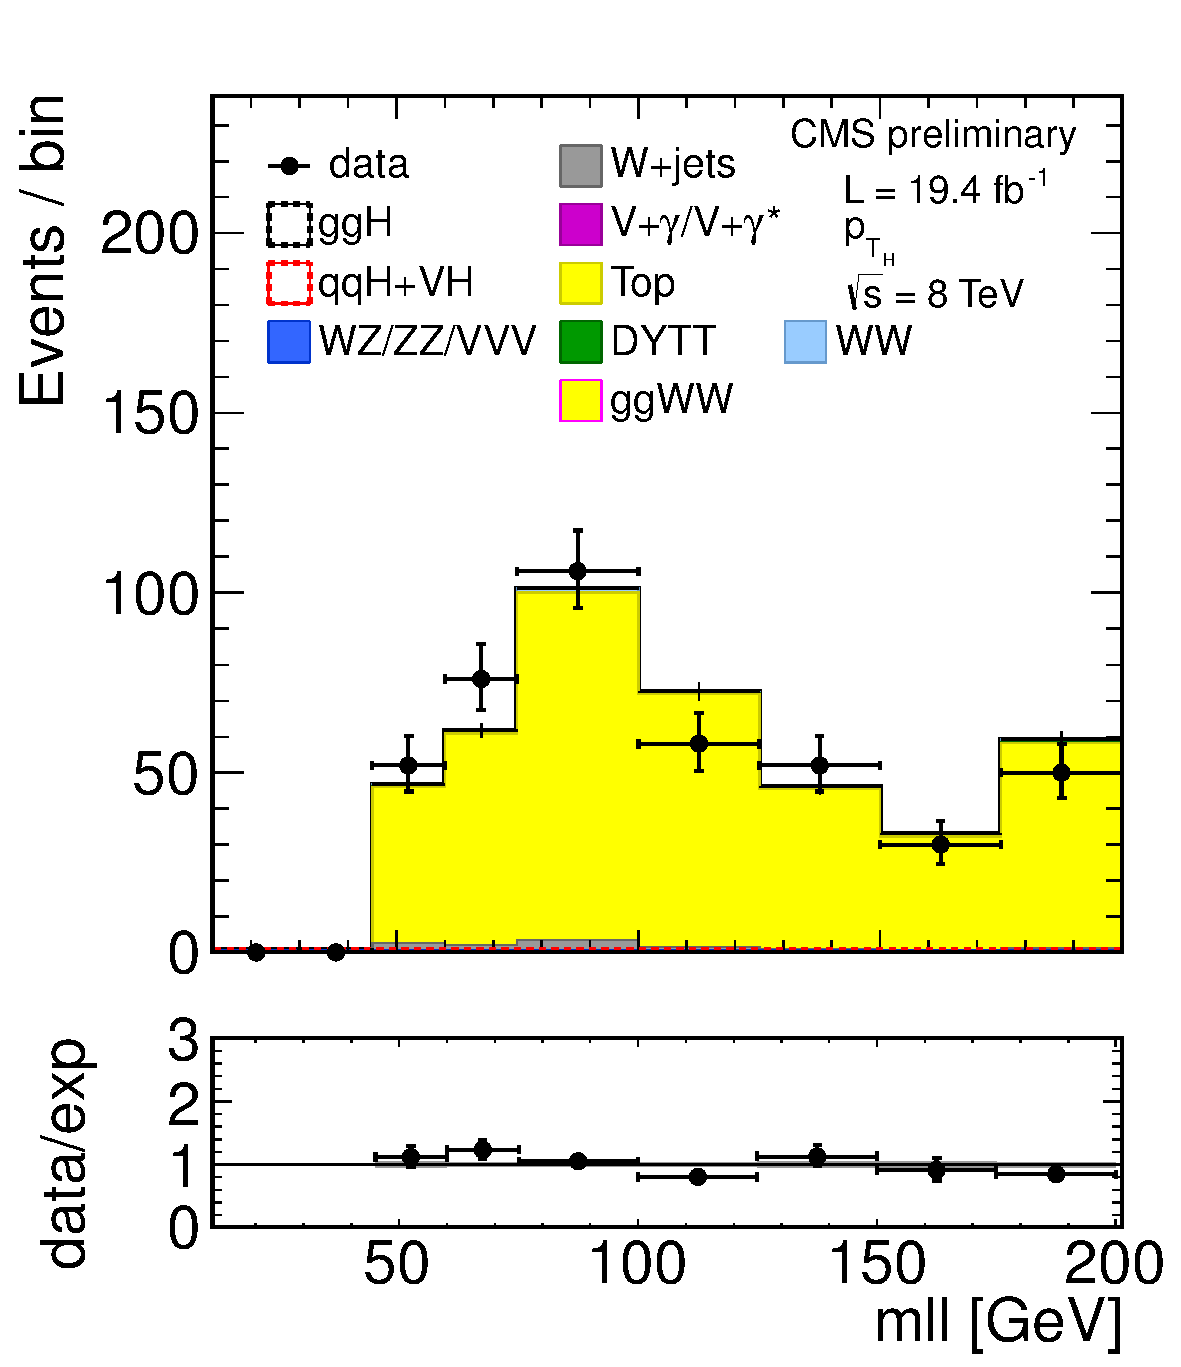
\includegraphics[width=0.35\textwidth]{images/mllBin0CtrlDD.pdf}}
\subfigure[$15\GeV<\pth<45\GeV$]{\includegraphics[width=0.35\textwidth]{images/mllBin1CtrlDD.pdf}}

\subfigure[$45\GeV<\pth<85\GeV$]{\includegraphics[width=0.35\textwidth]{images/mllBin2CtrlDD.pdf}}
\subfigure[$85\GeV<\pth<125\GeV$]{\includegraphics[width=0.35\textwidth]{images/mllBin3CtrlDD.pdf}}

\subfigure[$125\GeV<\pth<165\GeV$]{\includegraphics[width=0.35\textwidth]{images/mllBin4CtrlDD.pdf}}
\subfigure[$\pth>165\GeV$]{\includegraphics[width=0.35\textwidth]{images/mllBin5CtrlDD.pdf}}
\caption{$\mll$ distributions in the CtrlDD region for the different $\pth$ bins.\label{fig:mllCtrlDD}}
\end{figure}

























\clearpage
\subsection{WW background \label{sec:WWBackground}}

For what the $\mathrm{qq\to W^{+}W^{-}}$ background shape is concerned, the prediction from the simulation is used.
This background is divided into six different parts, corresponding to the six \pth bins defined in the analysis. The normalization of the $\mathrm{qq\to W^{+}W^{-}}$ background is left free to float in each bin, in such a way to adjust it in order to match the data during the fit procedure. In this way we minimize the shape difference between the $p_\mathrm{T}^\mathrm{WW}$ theory prediction and the distribution provided by the simulation, in our case the \textsc{Madgraph} generator.\\
In figure \ref{fig:ww_wwnlo} a comparison is shown between the $p_\mathrm{T}^\mathrm{WW}$ spectra of two different $\mathrm{qq\to W^{+}W^{-}}$ samples: one obtained with the \textsc{Madgraph} generator and the other after applying to the same distribution a reweighting in order to match the theoretical prediction at NLO+NNLL precision.

\begin{figure}[b]
\centering
\includegraphics[width=0.7\textwidth]{images/WWnlo/WW_WWnlo.pdf}
\caption{Comparison between the $p_\mathrm{T}^\mathrm{WW}$ distributions obtained with two different MC generators: the blue line corresponds to the \textsc{Madgraph} generator and the red line refers to he same sample in which a reweighting has been applied in order to match the theoretical prediction at NLO+NNLL precision. }\label{fig:ww_wwnlo}
\end{figure}

A shape discrepancy can be clearly observed and the effect becomes larger at high values of \pth.
In order to assess the effect of this discrepancy on the shapes of the variables used for the signal extraction, \mll and \mt, the shapes have been checked in all \pth bins, comparing different MC samples. The \textsc{Madgraph} sample used for the nominal shape is compared to the \textsc{Madgraph} sample with NLO+NNLL  reweighting, a \textsc{Powheg} sample with NLO accuracy and an \textsc{aMC@NLO} sample.
The results of this comparison are shown in figures \ref{fig:ww_mll} and \ref{fig:ww_mth}. The shape discrepancy among the different models is included as an additional systematic uncertainty.

\begin{figure}[htb]
\centering
\subfigure[$0<\pth<15$\GeV]{\includegraphics[width=0.45\textwidth]{images/WWnlo/mllBin1.pdf}}
\subfigure[$15<\pth<45$\GeV]{\includegraphics[width=0.45\textwidth]{images/WWnlo/mllBin2.pdf}}\\
\subfigure[$45<\pth<85$\GeV]{\includegraphics[width=0.45\textwidth]{images/WWnlo/mllBin3.pdf}}
\subfigure[$85<\pth<125$\GeV]{\includegraphics[width=0.45\textwidth]{images/WWnlo/mllBin4.pdf}}\\
\subfigure[$125<\pth<165$\GeV]{\includegraphics[width=0.45\textwidth]{images/WWnlo/mllBin5.pdf}}
\subfigure[$\pth>165$\GeV]{\includegraphics[width=0.45\textwidth]{images/WWnlo/mllBin6.pdf}}\\
\caption{Comparison between the default WW background sample and other theoretical models for the \mll distributions in every \pth bin.\label{fig:ww_mll}}
\end{figure}

\begin{figure}[htb]
\centering
\subfigure[$0<\pth<15$\GeV]{\includegraphics[width=0.45\textwidth]{images/WWnlo/mthBin1.pdf}}
\subfigure[$15<\pth<45$\GeV]{\includegraphics[width=0.45\textwidth]{images/WWnlo/mthBin2.pdf}}\\
\subfigure[$45<\pth<85$\GeV]{\includegraphics[width=0.45\textwidth]{images/WWnlo/mthBin3.pdf}}
\subfigure[$85<\pth<125$\GeV]{\includegraphics[width=0.45\textwidth]{images/WWnlo/mthBin4.pdf}}\\
\subfigure[$125<\pth<165$\GeV]{\includegraphics[width=0.45\textwidth]{images/WWnlo/mthBin5.pdf}}
\subfigure[$\pth>165$\GeV]{\includegraphics[width=0.45\textwidth]{images/WWnlo/mthBin6.pdf}}\\
\caption{Comparison between the default WW background sample and other theoretical models for the \mt distributions in every \pth bin.\label{fig:ww_mth}}
\end{figure}

The agreement of the \mll and \mt shapes between simulation and data for this background was checked in a signal-free control, defined selecting events with values of \mll greater than 60\GeV.

The gluon-induced WW process, i.e. gg$\to \mathrm{W^{+}W^{-}}$, has a sub-dominant contribution with respect to the quark-induced process, being the cross section ratio between the two of about 5\%. The \mll and \mt shapes for this background are taken from simulation while the cross section is scaled to the approximate NLO calculation~\cite{Bonvini:2013jha,Passarino:2013bha}.












































\subsection{Other backgrounds\label{sec:OtherBackgrounds}}

	%------------------------------------------------------------------------------------
	\subsubsection{Fake leptons background\label{sec:wjetsbkg}}	
	
Events in which W bosons are produced in association with jets, as well as multi-jet events, constitute a background for this analysis, because one or more jets can be misidentified as leptons. The rate at which jets are misidentified as leptons may be not accurately described in simulation, hence a data driven method is used to estimate this background. 
	
The idea is to estimate the background containing one or two fake leptons selecting events with relaxed lepton quality criteria, i.e. looser with respect to the selections used at the analysis level, and computing the efficiencies for real and fake leptons to pass the tight lepton quality requirements of the analysis. 
A data-driven approach is pursued to estimate this background. A set of loosely selected lepton-like objects, referred to as the ``fakeable object' or ``denominator'' from here on, is defined in a data set of events dominated by dijet production.
To measure the fake rate we count how many fakeable objects pass the full lepton selection 
of the analysis, parameterized as a function of the phase space of the fakeable lepton, therefore 
it is extracted in bins of $\eta$ and \pt.
The ratio of the fully identified lepton, referred as ``numerator'', to the 
fakeable objects is taken as the probability for a fakeable object to fake a lepton:

\begin{equation} \label{eq:fake_rate}
{Fake\ Rate } = \frac{\# of \ fully \ reconstructed \ leptons}{\# of \ fakeable \ objects} 
\end{equation}

It is then used to extrapolate from the loose leptons sample to a sample of leptons satisfying the  
full selection.

The definition of the denominator is of large impact in the systematic uncertainties related to this method. For the 2012 data taking period a summary of the selections used for the numerator and the denominator of Eq.~\eqref{eq:fake_rate} is shown below for electrons and muons respectively.
For electrons the denominator is defined by the following requirements:

\begin{itemize}
\item $\sigma_\mathrm{i\eta i\eta} < 0.01 (0.03)$ for barrel (endcap);
\item $|\Delta\phi_\mathrm{in}| < 0.15 (0.10)$ for barrel (endcap);
\item $|\Delta\eta_\mathrm{in}| < 0.007 (0.009)$ for barrel (endcap);
\item $H/E < 0.12 (0.10)$ for barrel (endcap);
\item electron conversion rejection;
\item $|d_0| < 0.02$\,cm;
\item $\frac{\sum_\mathrm{trk}E_\mathrm{T}}{\pt^\mathrm{ele}} < 0.2$;
\item $\frac{\sum_\mathrm{ECAL}E_\mathrm{T}}{\pt^\mathrm{ele}} < 0.2$;
\item $\frac{\sum_\mathrm{HCAL}E_\mathrm{T}}{\pt^\mathrm{ele}} < 0.2$.
\end{itemize}

For muons the selection are loosened with respect to the tight analysis selection requiring that:

\begin{itemize}
\item $|d_0| < 0.02$\,cm;
\item MVA isolation output $> -0.6$.
\end{itemize}

%shown in Table~\ref{tab:fake_muons} and \ref{tab_fake_electrons} for muons and electrons respectively.

%\begin{table}
%\centering
%\begin{tabular}{c c c}
%\hline
%Selection & Numerator & Denominator \\
%\hline\hline
%Muon ID & Global Muon + Tracker Muon & Tracker Muon \\
%\pt     & $\pt>20$\GeV & $\pt>20$\GeV \\
%$\eta$  & $|\eta|<2.4$ & $|\eta|<2.4$ \\
%Isolation & $(\mathrm{trackIso+caloIso})/\pt < 0.15$ & $(\mathrm{trackIso+caloIso})/\pt < 1$ \\
%\# inner tracker hits & $\mathrm{\# hits} > 10$ & $\mathrm{\# hits} > 10$ \\
%\# pixel hits & $\mathrm{\# hits} > 0$ & $\mathrm{\# hits} > 0$ \\
%Global $\chi^2$ & $\chi^2/\mathrm{ndof} < 10$ & -- \\
%$d0$ & $d0 < 0.02$\,cm & $d0 < 0.02$\,cm \\
%$dz$ & $dz < 1$\,cm & $dz < 1$\,cm \\
%\# valid SA hits & $>0$ & -- \\
%\# muon stations & $>1$ & -- \\
%\hline
%\end{tabular}
%\caption{Numerator and denominator selections for muons.\label{tab:fake_muons}}
%\end{table}

The dijet enriched data set used for the fake rate measurement, which is selected using single lepton triggers with low \pt thresholds, it is not a pure sample containing just fake leptons, but may still contain prompt leptons coming from the W and Z boson decays. To reject muons from the W decay, the events are required to have $\MET<20$\GeV and a W transverse mass below 20\GeV as well. Muons from the Z decay are instead remove requiring $m_{\mu\mu}>20$\GeV and $m_{\mu\mu} \notin [76,106]$\GeV. For electrons the Z mass peak veto is enlarged to $m_\mathrm{ee} \notin [60,120]$\GeV. Finally both electrons and muons are required to be isolated from the leading jet in the event, i.e. $\Delta\phi(\ell,j)>1$. The residual prompt lepton contamination from EW processes such as W/Z+jets production, which can bias the fake rate measurement, is estimated using simulation and subtracted from both the numerator and denominator. The contamination from EW processes is different for the numerator and denominator and is particularly important for relatively high lepton \pt values.

In addition to the fake rate, also a prompt lepton rate is evaluated, defined as the probability of a prompt lepton passing the loose requirements to also pass the tight analysis selections.
The prompt rate is also measured in data, defining a control region enriched in $\mathrm{Z} \to \ell\ell$ events, selecting dilepton events with an invariant mass of the two leptons in the Z peak mass region.

Both the fake and prompt rate are used to reweight the data samples used in the analysis in order to obtain directly from data the contribution of the fake lepton background. The method to apply those rates is explained below in the simple case of just one lepton in the data sample, i.e. data selected by single lepton triggers, but can be straightforwardly generalized to more complex situations.
Suppose that the total number of leptons passing the loose requirements, $N_\ell$, is made up of $N_p$ prompt and $N_f$ fake leptons. $N_p$ and $N_f$ cannot be directly measured but one can measure the number of events where no leptons, $N_{t0}$, or one lepton, $N_{t1}$, pass the tight analysis requirement. These numbers are related by the following equations:

\begin{equation}\label{eq:fake_single_lep}
\begin{gathered}
    N_\ell = N_p + N_f = N_{t0} + N_{t1}\\
    N_{t0} = (1-p)N_p + (1-f)N_f\\
    N_{t1} = pN_p + fN_f
\end{gathered}
\end{equation}

where $p$ and $f$ are the prompt and fake rates respectively. Equation~\eqref{eq:fake_single_lep} can be inverted to obtain the number of prompt and fake leptons:

\begin{equation}\label{eq:fake_prompt}
\begin{gathered}
    N_p = \frac{1}{p-f}\left[ (1-f)N_{t1} - fN_{t0}  \right]\\
    N_f = \frac{1}{p-f}\left[ pN_{t0} - (1-p)N_{t1}  \right]\\
\end{gathered}
\end{equation}

The systematic uncertainty is evaluated by varying the jet thresholds in the di-jet control sample, and by
performing a closure test in the same-sign data sample (see~\cite{AN-2013-022}) \textcolor{red}{REFERENZE}. In both cases it is about 36\%.

	%-------------------------------------------------------------------------------
	\subsubsection{Drell-Yan to \texorpdfstring{$\tau\tau$}{tau tau} background\label{sec:DYtautaubkg}}


The low \MET threshold in e$\mu$ final state
requires the consideration of the contribution from 
\dytt\, that is in fact estimated from data.
This is accomplished by using 
\dymm events and replacing muons with a simulated
$\tau\to l\nu_\tau\bar{\nu_e}$ decay \cite{AN-2011-020} \textcolor{red}{REFERENZE}.\\
After replacing muons from \dymm decays with simulated $\tau$ decays,
the set of pseudo \dytt events undergoes the reconstruction step.
 
Good agreement in kinematic distributions for this sample
and a MC based \dytt sample is found.
The global normalization of pseudo \dytt events is 
checked in the low \mt spectrum where a rather pure
\dytt sample is expected.


	%-------------------------------------------------------------------------------
	\subsubsection{ZZ, WZ and W\texorpdfstring{$\gamma$}{gamma} backgrounds\label{sec:otherbkg}}

The WZ and ZZ backgrounds are partially estimated from data when the two
selected leptons come from the same Z boson. If the leptons come from different
bosons the contribution is expected to be small. The WZ component is largely
rejected by requiring only two high \pt isolated leptons in the event. 
%The missing energy requirement makes the ZZ~$\to 4\ell$ component almost negligible.
%As the extra lepton veto and the \met cuts do not remove the ZZ~$\to 2\ell 2\nu$
%decays, a non-negligible fraction of these events survives the selection for $ee$ and $\mu\mu$ channels only. 

The W+$\gamma^{(*)}$ background, where the photon decays to an electron-positron pair,
is expected to be very small, thanks to the stringent photon conversion
requirements.
 Since the WZ simulated sample has a generation level cut on the
di-lepton invariant mass ($m_{\ell\ell} >$ 12~\GeV) and the cross-section raises
quickly with the lowering of this threshold, a dedicated \textsc{Madgraph} sample has
been produced with lower momentum cuts on two of the three leptons
($\pt > 5$~\GeV) and no cut on the third one. The surviving contribution
estimated with this sample is still very small, and since the uncertainty on the
cross-section for the covered phase space is large, a conservative 100\%
uncertainty has been given to it. 
A $k$-factor for W+$\gamma^{*}$ of $1.5\pm0.5$ based on a dedicated measurement of 
tri-lepton decays, W+$\gamma^{*} \to e\mu\mu$ and W+$\gamma^{*} \to \mu\mu\mu$,
is applied~\cite{WGammaStarStudy} \textcolor{red}{REFERENZE}. 
The contribution of W+$\gamma^{(*)}$ is also
constrained by a closure test with same sign leptons on data, which reveals a
good compatibility of the data with the expected background.


%\clearpage
%\section{Systematic uncertainties}
%%%%%%%%%%%%%%%%%%%%%%%%%%%%%%%%%%%%%%%%%%%%%%%%%%%%%%%%%%%%%%%%%%%%%%
\label{sec:Systematics}

Systematic uncertainties play an important role in this analysis where
no strong mass peak is expected due to the presence of undetected
neutrinos in the final state. They arise from three sources: background predictions, experimental measurements, and theoretical uncertainties. One of the most important sources is the normalization of the backgrounds that are estimated on data control samples whenever is possible.

The systematic uncertainties can affect the measured signal strengths in different ways. The uncertainties on the background predictions can be divided in those affecting the background cross section, the (\mll, \mt) shape or both. As an example, systematic uncertainties changing the background cross section are the ones related to the background data-driven estimation, while the b tagging uncertainties only have an effect on the (\mll, \mt) shape. Uncertainties such as lepton energy scale can instead affect both normalization and shape. Also, uncertainties affecting the signal (\mll, \mt) shape reflect on an uncertainty on the measured signal strength. 

A summary of the main sources of systematic uncertainty and the corresponding estimate is reported in Table~\ref{tab:Systematics}. A brief description of each source of systematic uncertainty is discussed in the following sections.

The uncertainties related to the unfolding procedure are treated separately and are discussed in Sec.~\ref{sec:uncunf}.

\begin{table}[h]
\small{
  \begin{center}
  \caption{Main sources of systematic uncertainties and their estimate. The
  first category reports the uncertainties on the normalization of background
  contributions. The experimental and theoretical uncertainties refer to the
  effect on signal yields. A range is specified if the uncertainty varies
  across the $\pth$ bins.}
  \label{tab:Systematics}
  \begin{tabular}{cc}
  \hline\hline
  \multicolumn{2}{c} {\bf{Uncertainties in backgrounds contributions}} \\
  \hline
  Source  & Uncertainty \\
  \hline
  $\rm{t\bar{t}}$, tW      & 20--50$\%$ \\
  W+jets              & $40\%$ \\
  WZ, ZZ              & $4\%$ \\
  W$\gamma^{*}$, W$\gamma$  & $30\%$ \\
  \hline\hline
  \multicolumn{2}{c} {\bf{Effect of the experimental uncertainties on the signal and background yields}}\\
  \hline
  Source & Uncertainty\\
  \hline
  Integrated luminosity        & $2.6\%$ \\
  Trigger efficiency           & 1--2$\%$\\
  Lepton reconstruction and identification & 3--4$\%$\\
  Lepton energy scale          & 2--4$\%$ \\
  \MET modelling          & $2\%$ \\
  Jet energy scale             & $10\%$ \\
  Pileup multiplicity          & $2\%$ \\
  b mistag modelling	       & $3\%$ \\	
  \hline\hline
  \multicolumn{2}{c}{\bf{Effect of the theoretical uncertainties on signal yield}}\\
  \hline
  Source & Uncertainty \\
  \hline
  b jet veto scale factor              & 1--2$\%$\\
  PDF                                  & $1\%$ \\
  WW background shape                  & $1\%$\\
  \hline
  \end{tabular}
  \end{center}
}
\end{table}


%-------------------------------------------------------------------------------
\subsection{Background predictions uncertainties}
%-------------------------------------------------------------------------------

The signal extraction is performed fitting the estimated background contributions and subtracting them to the event counts in data. Therefore, the uncertainties on the background predictions indirectly reflect as uncertainties on the signal measurements. A list of the most important background uncertainties is given below.

\begin{itemize}
\item {\bf\boldmath \ttbar and tW backgrounds:}    
the shapes of these backgrounds are corrected for different b tagging efficiency in data and simulation, and the normalization is taken from data in a top quark enriched control region independently in each \pth bin, as explained in Sec.~\ref{sec:TTBackground}. The uncertainties related to this procedure arise from the sample size in the control regions for each \pth bin, and are embedded in the $\alpha$ factors used to extrapolate
the top quark background normalization from the control region to the signal region. They vary from 20\% to 50\% depending on the \pth bin.
   
The simulated samples include both \ttbar and tW processes, a systematic uncertainty related to the tW$/$\ttbar fraction has been included.
In fact, a relative variation of the contribution of these two processes could modify the shape of the simulated sample, and is thus included as a shape uncertainty affecting the (\mll, \mt) shape in each \pth bin in a correlated way. 

\item {\bf \boldmath{WW background}:} 
due to the fact that the WW background (\mll, \mt) shape is entirely taken from simulation, the analysis is relying on theoretical models and can thus be affected by their uncertainties. Especially higher order QCD radiative effects have an influence on the generated WW shape. To study this impact, the shapes of the distributions produced with the \textsc{MadGraph} generator are compared to the ones produced with \textsc{mc@nlo} and other generators (see Sec.~\ref{sec:WWBackground}). The comparison is performed separately in each bin of \pth and the uncertainty includes shape differences originating from the renormalization and factorization scale choice. The effect on the signal strengths is found to be of the order of 1\%.
  
\item {\bf\boldmath W+jets background:} 
the systematic uncertainties on the W+jets background arise from the estimation method explained in Sec.~\ref{sec:wjetsbkg}. This uncertainty has two sources: the dependence of $\varepsilon_\mathrm{pass}$ on the sample composition, and the method. The first source is estimated by modifying the jet \pt threshold in the QCD multijet sample, which modifies the jet sample composition.  The uncertainty in the method is obtained from a closure test, where $\varepsilon_\mathrm{pass}$ is derived from simulated QCD multijet events and applied to simulated samples to predict the number of background events. The total uncertainty in $\varepsilon_\mathrm{pass}$, including the statistical precision of the control sample, is of the order of 40\%.
 
\item {\bf\boldmath Diboson backgrounds:} 
these backgrounds are expected to give a small contribution in the signal phase space. Uncertainties on the cross sections reported in \cite{xsecSM,bib:ellis} are 4\% for WZ and 2.5\% for ZZ. A 30\% uncertainty is assigned to the $W\gamma$ \cite{WgammaXsec} yield and another 30\% on $W\gamma^{*}$ contribution according to the uncertainty on the normalization study (see Sec.~\ref{sec:diboson}).
      
\end{itemize}

%-------------------------------------------------------------------------------
\subsection{Experimental uncertainties \label{subsec:expsyst}}
%-------------------------------------------------------------------------------

The following experimental systematic sources have been taken into account:

\begin{itemize}
\item {\bf Luminosity:} using the CMS online luminosity monitoring system, the uncertainty on the integrated luminosity (19.4\ifb) collected during the 2012 data taking period is found to be of $2.6\%$.

\item {\bf Trigger efficiency:} the uncertainties for both electrons and muons, estimated as described in Sec.~\ref{sec:trigeff}, are at 1-2\% level.

\item {\bf Lepton reconstruction and identification efficiency:} 
this uncertainty is estimated with the Tag and Probe technique described in Sec.~\ref{sec:leptonID}, resulting in a 4\% uncertainty for electrons and 3\% for muons.

\item {\bf Muon momentum and electron energy scale:} 
the momentum scale of leptons has relatively large uncertainties due to different detector effects, as explained in Sec.~\ref{sec:leptonID}. For electrons a scale  uncertainty of 2\% for the barrel, and 4\% for the endcaps respectively, is assigned. For muons, a momentum scale uncertainty of 1.5\%, independent on the muon pseudorapidity, is assigned.

\item {\bf {\boldmath \MET} modelling:} 
  the \MET measurement is affected by the possible mis-measurement of 
  individual particles addressed above, as well as the additional contributions 
  from the pile-up interactions, as described in Sec.~\ref{sec:met}. 
  The effect of the missing transverse momentum resolution on the event selection
  is studied by applying a Gaussian smearing of 10\% on the $x$- and
  $y$-components of the missing transverse momentum. All correlated variables,
  like the transverse mass, are recalculated. The effect is found to be around 2\%.

\item {\bf Jet energy scale (JES) uncertainties:} 
  JES uncertainties affect both the jet multiplicity and the jet kinematic variables, reflecting also on the (\mll, \mt) shape.
  This uncertainty is estimated varying the kinematics of the reconstructed jets within the uncertainties on the JES (which depend on $\eta$ and $\pt$ of the jet) described in Sec.~\ref{sec:jets}, and recomputing all the correlated variables, like \mll and \mt.

\item {\bf b-jets misidentification modelling:}
a fraction of signal events is rejected because erroneously identified as b-jets by the b tagging algorithms. The misidentification probability, as measured with the Tag and Probe technique described in Sec.~\ref{sec:ScaleFactors}, has an uncertainty related to different b tagging performance in data and simulation. This affects also non-top quark backgrounds.
          
\item {\bf Pileup multiplicity:} 
some of the variables used in the analysis are affected by the average number of pile up interactions. The simulated events have been reweighted according to the instantaneous luminosity measured on data. The error on the average number of pile up interactions measured in data and the simulation of the modelling and physics aspects of the pile up simulation provide an uncertainty of at most 5\% on the distribution used in the reweighting procedure. This uncertainty is propagated through all the analysis, and the estimated uncertainty on the signal strengths do not exceed 2\%.

\end{itemize}

%-------------------------------------------------------------------------------
\subsection{Theoretical uncertainties \label{subsec:thsyst}}
%-------------------------------------------------------------------------------

Theoretical uncertainties generally arise from missing higher-order corrections in QCD and PDF uncertainties. These uncertainties can affect both the cross section and the (\mll, \mt) shape of the background predictions, as well as the shape of the signal model.

\begin{itemize}

\item {\bf QCD scale uncertainties:}
the uncertainties on the total cross sections due to the choice of the renormalization and factorization scale are assigned to simulation-driven backgrounds. For the signal processes these uncertainties are separated in two categories: those affecting the selection efficiency and those affecting the jet bin fractions. The effect of renormalization and factorization scale on the selection efficiency is of the order of 2\% for all processes. Although this analysis is inclusive in number of jets, the effect of the QCD scales variation on the jet bin migrations has to be taken into account because of the b tagging veto efficiency. Indeed, the b tagging veto efficiency is not flat as a function of jet multiplicity not \pth, as shown in Fig.~\ref{fig:bveto_eff}, therefore introducing a dependence of the selection efficiency on the number of jets on the event.
In order to take into account this effect, an uncertainty on the ggH production mode has been included according to the Stewart-Tackman method, following the recipe proposed in Refs.~\cite{Stewart:2011cf,Heinemeyer:2013tqa}. The effect on the signal strengths is found to be of the order of 1--2\%.

\item {\bf PDFs uncertainties:} 
the utilization of different PDF sets can affect the (\mll, \mt) shapes of the signal contributions, as well as the normalization and shape of the background predictions. The uncertainty related due to the variations in the choice of PDFs is considered following the PDF4LHC~\cite{Alekhin:2011sk,Botje:2011sn} prescription, using CT10, NNPDF2.1~\cite{Ball:2011mu} and MSTW2008~\cite{Martin:2009iq} PDF sets. The effect on the signal strengths is found to be of at most 1\%.

\end{itemize} 

\begin{comment}
\subsubsection{Jet multiplicity uncertainty} \label{subsec:stewart-tackman}

The jet bin uncertainty on the ggH production mode has been evaluated using the Stewart-Tackman method, following the recipe proposed in Refs.~\cite{Stewart:2011cf,Heinemeyer:2013tqa}.
Three independent nuisance parameters have to be associated with the inclusive ggH production cross sections $\sigma_{\geq 0}$, $\sigma_{\geq 1}$ and $\sigma_{\geq 2}$, which corresponds to the cross sections with $\geq 0$ jets, $\geq 1$ jet and $\geq 2$ jets respectively. According to the agreement on the treatment of uncertainties in the combination of ATLAS and CMS results~\cite{ATLAS:2011tau}, these nuisance parameters are labelled as \emph{QCDscale\_ggH}, \emph{QCDscale\_ggH1in} and \emph{QCDscale\_ggH2in}. However, in case the analysis is split in exclusive jet multiplicity bins, the jet bin uncertainties can be evaluated taking into account the correct correlations among the three nuisances following the Stewart-Tackman prescription.
Even though this analysis is inclusive in number of jets, the jet binning uncertainties must be included due to the presence of the b-jet veto, that introduces a dependency of the selection efficiency on the number of jets in the event. The veto efficiency has been evaluated in all the \pth bins defined in the analysis and as a function of jets multiplicity. The results are shown in Figs.~\ref{fig:veto_eff_pth} and \ref{fig:veto_eff_njet}. The drop of the veto efficiency at high values of \pth is due to the correlation with jets multiplicity.
	 	
\begin{figure}[htb]
\centering
	\subfigure[]{
		\centering
		\includegraphics[width=0.45\textwidth]{images/eff_vs_pth.pdf}
		\label{fig:veto_eff_pth}
	}
	\subfigure[]{
		\centering
		\includegraphics[width=0.45\textwidth]{images/eff_vs_jet.pdf}
		\label{fig:veto_eff_njet}
	}
\caption{(a) Efficiency of the b-tagging veto in different bins of \pth. (b) Efficiency of the b-tagging veto in different bins of \pth, as a function of number of jets.}\label{fig:bveto_eff}
\end{figure}

The first step of this procedure is to take the inclusive ggH cross section, $\sigma_\mathrm{ggH}$, and to convert the relative QCD up/down scale uncertainties, $\epsilon_+$ and $\epsilon_-$, to a log-normal uncertainty, i.e. $\kappa = \sqrt{\exp{(\epsilon_+)}\cdot \exp{(\epsilon_-)}}$. The exclusive cross sections, $\sigma_0$, $\sigma_1$ and $\sigma_2$, can be calculated starting from $\sigma_\mathrm{ggH}$ and using the selection efficiencies for the three jet bins. For every exclusive cross section the corresponding relative uncertainty is computed varying the renormalization ($\mu_R$) and factorization ($\mu_F$) scales independently of a factor 2 and $1/2$, and taking the cross section value corresponding to half of the maximum variation. The inclusive cross sections are then obtained summing the exclusive cross sections and propagating the uncertainties, i.e. $\sigma_{\geq 0 } = \sigma_0 + \sigma_1 + \sigma_2$, $\sigma_{\geq 1} = \sigma_1 + \sigma_2$, $\sigma_{\geq 2} = \sigma_2$.

The three nuisance parameters, including all the proper correlations among the jet bins, are defined according to Table~\ref{table:jet_binning_theory}, where the $f_n$ constants represent the exclusive theoretical $n$ jet bin fractions, i.e. $f_0 = \sigma_0/\sigma_{\geq 0}$, $f_1 = \sigma_1/\sigma_{\geq 0}$, $f_2 = \sigma_2/\sigma_{\geq 0}$.

\begin{table}[h]
\caption{Numerical calculation for the systematic uncertainties of jet binning.}
\label{table:jet_binning_theory}
\begin{center}
\begin{tabular}{|l|c|c|c|}
\hline
Nuisance parameter & 0-jet bin                                              & 1-jet bin                                            & 2-jet bin \\ 
\hline
&&& \\
QCDscale\_ggH          & $\Delta^0_{\geq 0} = (\kappa_{\ge 0})^{\frac{1}{f_0}} $    &      & \\ 
&&&\\\hline
&&&\\
QCDscale\_ggH1in       & $\Delta^0_{\geq 1} = (\kappa_{\ge 1})^{- \frac{f_1 + f_2}{f_0}} $ & $\Delta^1_{\geq 1} = (\kappa_{\ge 1})^{\frac{f_1 + f_2}{f_1}} $ & \\ 
&&&\\ \hline
&&&\\
QCDscale\_ggH2in        &                                                        & $\Delta^1_{\geq 2} = (\kappa_{\ge 2})^{- \frac{f_2}{f_1}} $     & $\Delta^2_{\geq 2} = (\kappa_{\ge 2})$ \\ 
&&&\\\hline

\end{tabular}
\end{center}
\end{table}

The nuisance parameters reported in table \ref{table:jet_binning_theory} have then been calculated for each \pth bin embedding the b-jet veto efficiency and using the following formulas:
\begin{equation}
\emph{QCDscale\_ggH}=\frac{\Delta^0_{\geq 0}\cdot f_{0}\cdot \varepsilon_{0}+\Delta^0_{\geq 1}\cdot f_{1}\cdot\varepsilon_{1}}{\Delta^0_{\geq 0}\cdot f_{0}\cdot \varepsilon_{0}+\Delta^0_{\geq 1}\cdot f_{1}\cdot \varepsilon_{0}} \quad,
\end{equation}
\begin{equation}
\emph{QCDscale\_ggH1in}=\frac{\Delta^1_{\geq 1}\cdot f_{1}\cdot \varepsilon_{1}+\Delta^1_{\geq 2}\cdot f_{2}\cdot \varepsilon_{2}}{\Delta^1_{\geq 1}\cdot f_{1} \cdot \varepsilon_{1}+\Delta^1_{\geq 2}\cdot f_{2}\cdot \varepsilon_{1}} \quad,
\end{equation}
\begin{equation}
QCDscale\_ggH2in=1 \quad,
\end{equation}
where $\varepsilon_0$, $\varepsilon_1$ and $\varepsilon_2$ are the selection efficiencies for the three jet categories.
These nuisance parameters are expected to be equal to one in case the efficiency is independent on the number of jets, i.e if $\varepsilon_0 = \varepsilon_1 = \varepsilon_2$.\\
The numerical values obtained following this procedure are reported in Table~\ref{table:jet_binning_meas} for each \pth bin.

\begin{table}[h]
\caption{Values of the jet binning nuisance parameters for different \pth bins.}
\label{table:jet_binning_meas}
\begin{center}
\begin{tabular}{ccccccc}
\toprule
\multirow{2}{*}{Nuisance parameter} & \multicolumn{6}{c}{\pth bin [GeV]} \\
& [0-15] & [15-45] & [45-85] & [85-125] & [125-165] & [165-$\infty$]\\
\midrule
QCDscale\_ggH  & 0.998  &   0.993  &   0.989  &   1.000  &   1.000   &  1.000 \\
QCDscale\_ggH1in &0.997   &  0.993  &   0.984  &   0.975 &    0.946 &    0.974  \\
\bottomrule
\end{tabular}
\end{center}
\end{table}
\end{comment}

%-------------------------------------------------------------------------------
\subsection{Statistics uncertainty of the simulated samples}
%-------------------------------------------------------------------------------

Due to the large range of weights used to correct the simulated distributions in order to
match those in data, the effective size of the simulated samples are sometimes smaller than
the actual number of events in the sample.
The uncertainties due to the finite statistics of the simulated samples are taken into account and propagated through the final result. Their effect on the signal strengths is found to be negligible.

%-------------------------------------------------------------------------------
\subsection{Treatment of systematic uncertainties in the analysis}\label{sec:syst_treatment}
%-------------------------------------------------------------------------------

As explained before, one can distinguish between normalization uncertainties, where a systematic effect is changing the normalization of a given process assuming the (\mll, \mt) shape is not affected, and shape uncertainties where the actual change in the (\mll, \mt) shape of the process is taken into account. The normalization uncertainties enter the analysis as constant normalization factors, whereas for shape uncertainties the nominal and the $+1\sigma$ and $-1\sigma$ shapes enter the analysis in form of three histograms with the same normalization. 

Effects from experimental uncertainties are studied by applying a scaling and smearing of certain variables of the physics objects, followed by a subsequent recalculation of all the correlated variables. This is done for simulation, to account for possible systematic mis-measurements of the data. All experimental sources from Section~\ref{subsec:expsyst} but luminosity are treated both as normalization and shape uncertainties. For background with a data-driven normalization estimation, only the shape uncertainty is considered.

%\clearpage
%\section{Control Plots}
%%%%%%%%%%%%%%%%%%%%%%%%%%%%%%%%%%%%%%%%%%%%%%%%%%%%%%%%%%%%%%%%%%%%%%
\label{sec:ControlPlots}

\subsection{Signal and background yields}\label{subsec:yields}
In table \ref{table:yields} are reported the expected number of events for signals and backgrounds after the full analysis selection. The uncertainties in the expected number of events correspond to the prefit nuisances effect affecting each process. As can be observed, signals are splitted into different categories depending on the production mode: gluon fusion (ggH), VBF (qqH) and VH (WH and ZH) which includes also ttH production. Each signal is again splitted in six different contributions related to the \pth bins. The total expected signal yield after the analysis selection is $382 \pm 7$ events.\\
For what the backgrounds are concerned, the WW has been splitted in bins of \pth and has been left free to float independently in each bin during the fit. For doing this a 100 \% uncertainty has been associated to the expected number of events in each bin, following a prior flat distribution (log uniform distribution). That is why the uncertainty on WW backgrounds and on total background yield are not reported in the table.\\
The Top background has been divided into two categories of events as explained in \ref{sec:TTBackground}: events with zero jets (Top0jet) and events with more than zero jets (Topge1jet). The yield in the first category has been extracted performing a data driven estimation in a control region. The latter category has been further splitted in the various \pth bins and a data driven estimation has been performed separately in each bin to avoid a shape mismodelling in the \pth distribution for this background.\\
The final signal to background ratio is around 3~\%, consistent with what illustrated in figure \ref{fig:cutflow}.

\begin{table}[htbp]
\begin{center}
 {
\small{
\setlength{\extrarowheight}{2pt}
  \caption{Signal prediction, background estimates and observed number of events in data are shown in each \pth{} bin for the signal after applying the analysis selection requirements. The total uncertainty on the number of events is reported. For signal processes, the yield related to the ggH are shown, separated with respect to the contribution of the other production mechanisms (XH=VBF+VH). The WW process includes both quark and gluon induced contribution, while the Top process takes into account both $\mathrm{t\bar t}$ and tW. }\label{table:yields}
\begin{tabular} {l c c c c c c}
  \hline \hline
$\mathbf{p}_{\rm \mathbf{T}}^{\rm \mathbf{H}} \left[\mathrm{\mathbf{GeV}}\right] $	&	\bf{0-15}	&	\bf{15-45}	&	\bf{45-85}	&	\bf{85-125}	&	\bf{125-165}	&	\bf{165-$\boldsymbol{\infty}$} \\ 	

\hline

ggH	&	$73\pm3$	&	$175\pm5$	&                $59\pm3$	&                $15\pm2$	&                $5.1\pm1.5$	&                $4.9\pm1.4$	\\
XH=VBF+VH	&	$4\pm2$ 	&	$15\pm4$ 	&		 $16\pm4$	&	         $8\pm2$ 	&		 $3.8\pm1.1$ 	&		 $3.0\pm0.8$    \\	
Out-of-fiducial & $9.2\pm0.5$   &       $19.9\pm0.7$    &      $11.4\pm0.6$    &    $4.4\pm0.3$   &     $1.6\pm0.2$   &   $2.4\pm0.2$ \\
Data 	&	2182	 	&         5305	 	&	         3042	 	& 	          1263	 	&	         431	 	& 	          343	 	\\
Total background &  	 $2124\pm128$	 &     $5170\pm321$	 &       $2947\pm293$	 &            $1266\pm175$	 &         $420\pm80$	 &              $336\pm74$	 \\

WW 	& 		$1616\pm107$	 &	 $3172\pm249$	 &	     $865\pm217$	 &	     $421\pm120$	 &	     $125\pm60$	 &		     $161\pm54$	 \\
Top 	&	$184\pm38$	&	                $1199\pm165$	&	                $1741\pm192$	&	                $735\pm125$	&	                $243\pm51$	& 	        $139\pm49$	\\
W+jets 	& $134\pm5$ 	&	         $455\pm10$ 	&	         $174\pm6$ 	&	         $48\pm4$ 	&	         $14\pm3$ 	&	         $9\pm3$ 	\\
WZ+ZZ+VVV & $34\pm4$ 	 &	$107\pm10$ 	&                $71\pm7$ 	&	         $29\pm5$ 	&                $14\pm3$ 	&     $13\pm4$ 	\\
\dytt 	&	$23\pm3$ 	&         $67\pm5$ 	&         $47\pm4$ 	&         $22\pm3$ 	&         $12\pm2$ 	&         $10\pm2$ 	\\
W$\gamma^{(*)}$	& $132\pm49$     &             $170\pm58$    &              $48\pm30$ &                  $12\pm9$ &                  $3\pm3$ &                 $5\pm10$ \\
\hline

\hline
  \end{tabular}
  }
  }

  \end{center}
\end{table}

\subsection{Control plots in the signal region}
In figure \ref{fig:control_plots} are reported the control plots in the signal region for the \mll~ distribution in all the \pth bins. Data points are superimposed to MC distributions only in the high \mll~ region (above 70~\GeV), where no signal is expected. The error bands shown in these plots correspond to the total prefit uncertainty, taking into account all the sources of error. The very large uncertainties are expected and are related to the 100~\% uncertainty assigned to the WW floating background. The error band will decrease once the fit will be performed, i.e using the postfit values of the nuisance parameters, and the WW yield will be adapted to data.
\begin{figure}[htb]
\centering
\subfigure[Bin1]{
\includegraphics[width=0.35\textwidth]{images/mllBin0.pdf}
}
\subfigure[Bin2]{
\includegraphics[width=0.35\textwidth]{images/mllBin1.pdf}
}
\\
\subfigure[Bin3]{
\includegraphics[width=0.35\textwidth]{images/mllBin2.pdf}
}
\subfigure[Bin4]{
\includegraphics[width=0.35\textwidth]{images/mllBin3.pdf}
}
\\
\subfigure[Bin5]{
\includegraphics[width=0.35\textwidth]{images/mllBin4.pdf}
}
\subfigure[Bin6]{
\includegraphics[width=0.35\textwidth]{images/mllBin5.pdf}
}
\caption{Control plots showing the \mll~distributions in every Higgs \pt bin. Data are superimposed in the region where the signal is expected to be negligible.}\label{fig:control_plots}

\end{figure}

As expected the Top background becomes more important while going to high values of \pth, accordingly to the higher jet multiplicity in that region. The discrepancy between MC prediction and data, especially for low values of Higgs \pt, is due WW background which in this plots is fixed to the MC cross section.


%\clearpage
%\section{Signal extraction}
%%%%%%%%%%%%%%%%%%%%%%%%%%%%%%%%%%%%%%%%%%%%%%%%%%%%%%%%%%%%%%%%%%%%%%
\label{sec:SignalExtraction}

In this section the fitting procedure as well as the measured signal and background yields are described.


\subsection{Fitting procedure}\label{sec:fit}

The signal, including ggH, VBF, and VH production mechanisms, is extracted in each bin of \pth{} by performing a binned maximum likelihood fit simultaneously in all \pth bins to a two-dimensional template for signal and background in the \mll--\mt plane.
The variables used for the two-dimensional template are chosen for their power to discriminate signal and background contributions. This is shown in Fig.~\ref{fig:2Dlegacy}, where the two-dimensional simulated distributions are shown for the signal and background processes in the 0 jets category. As can be observed, the signal contribution in the 0 jets category is mostly distributed in the low \mll region and for \mt values around 90--110\GeV. The background contribution, which is mainly owed to the WW, W+jets and \dytt production, is instead distributed in the high \mll region and for intermediate values of \mt (below 100\GeV).

\begin{figure}[htb]
\centering
\subfigure[]{\includegraphics[width=0.45\textwidth]{images/legacyPlots/2d_prefit_0j_125_sig_paper.pdf}}
\subfigure[]{\includegraphics[width=0.45\textwidth]{images/legacyPlots/2d_prefit_0j_125_bkg_paper.pdf}}
\caption{Two-dimensional \mll--\mt distribution for signal (a) and background (b) processes in the 0 jets category.\label{fig:2Dlegacy}}
\end{figure}

Six different signal strengths are extracted from the fit, one for each \pth~bin. The relative contributions of the different Higgs production mechanisms in the signal template are taken to be the same as in the SM. The sources of systematic uncertainty are considered as nuisance parameters in the fit.

The binning of the \mll and \mt templates is chosen to be:
\begin{itemize}
\item {\mll: $[12,30,45,60,75,100,125,150,175,200]$} 
\item {\mt: $[60,70,80,90,100,110,120,140,160,180,200,220,240,280]$}
\end{itemize}

To avoid a dependence of the results on the variables used for the template fit, \mll and \mt need to be uncorrelated with respect to \pth.
This has been verified and the correlation between the discriminating variables and \pth is shown in Fig.~\ref{fig:correlation_ggH} and Fig.~\ref{fig:correlation_vbf} for ggH and VBF production modes, respectively.

\begin{figure}[htb]
\centering
\subfigure[]{\includegraphics[width=0.45\textwidth]{images/correlationmll_ggH-v2.pdf}}
\subfigure[]{\includegraphics[width=0.45\textwidth]{images/correlationmth_ggH-v2.pdf}}
\caption{Correlation between $\pth$ and $\mll$ (a) and between \pth and \mt (b) after the full selection for the ggH production mode.\label{fig:correlation_ggH}}
\end{figure}

\begin{figure}[htb]
\centering
\subfigure[]{\includegraphics[width=0.45\textwidth]{images/correlationmll_vbf-v2.pdf}}
\subfigure[]{\includegraphics[width=0.45\textwidth]{images/correlationmth_vbf-v2.pdf}}
\caption{Correlation between \pth and \mll (a) and between \pth and \mt (b) after the full selection for the VBF production mode.\label{fig:correlation_vbf}}
\end{figure}

The signal strength $\mu$ in each bin, defined as the ratio between the measured cross section and the SM one, $\mu = \sigma/\sigma_\mathrm{SM}$, is allowed to float between -10 and +10, thus permitting negative values. This is mainly intended to allow future combinations with similar measurements without introducing any bias.

Because of detector resolution effects, some of the reconstructed $\hww$ signal events might originate from outside the fiducial phase space.  
These out-of-fiducial signal events cannot be precisely handled by the unfolding procedure and must be subtracted from the reconstructed spectrum. The \pth distribution of the out-of-fiducial signal events is taken from simulation, and each bin is multiplied by the corresponding measured signal strength before performing the subtraction. 

At the end, the number of events in each bin $i$ of the measured spectrum is:
\begin{equation}\label{eq:sig_yield}
N_i = \mu_i (s_i -f_i) \quad ,
\end{equation}

\noindent where $\mu_i$ is the measured signal strength, $s_i$ and $f_i$ are the total number of reconstructed signal events and the number of reconstructed out-of-fiducial signal events expected from simulation, respectively.

The fit makes use of the binned maximum likelihood approach. The likelihood function $\mathcal{L}$, restricted to the \pth bin $j$, can be written as:
\begin{equation}
\mathcal{L}(data|\mu_j,\theta) = Poisson(data|\mu_j \cdot s(\theta) + b(\theta)) \cdot p(\tilde{\theta} |\theta ) \quad ,
\end{equation}

\noindent where $Poisson(data|\mu_j \cdot s + b)$ is the product of the Poisson probabilities to observe $n_i$ events in bin $i$, i.e.:
\begin{equation}\label{eq:poisson}
\prod_i \frac{(\mu_j\cdot s_i + b_i)^{n_i}}{n_i !} e^{-\mu_j \cdot s_i - b_i} \quad.
\end{equation}

%\begin{equation}
%\mathcal{L}(\mu_j,\theta) = \prod_{i=0}^{N_\mathrm{bins}} \frac{(\mu_j s_i(\theta) + b_i(\theta))^{n_i}}{n_i!}e^{-\mu_j s_i(\theta) - b_i(\theta)} \cdot p(\tilde{\theta} |\theta ) \quad ,
%\end{equation}
Here $\mu_j$ is the signal strength in the bin $j$, i.e. the parameter of interest of the fit, which multiplies the signal yield. The index $i$ runs over the bins of the \mll-\mt two-dimensional histogram corresponding to the \pth bin $j$, $s_i$ and $b_i$ are the expected number of signal and background events respectively in bin $i$, and $n_i$ is the total number of observed events in bin $i$. The set of parameters $\theta$ represents the full suite of nuisance parameters used to incorporate the systematic uncertainties. Each nuisance parameter is constrained in the fit including the prior distribution functions $p(\tilde{\theta}|\theta)$ in the likelihood, where $\tilde{\theta}$ is the set of default values for the $\theta$ parameters~\cite{CMS-NOTE-2011-005}. For the major part of the nuisance parameters a log-normal prior distribution is used, with a standard deviation corresponding to the given systematic uncertainty. This is the optimal choice to describe uncertainties of definite positive observables, like cross sections, efficiencies, luminosity, etc. The usage of a gaussian distribution, under certain circumstances, would indeed allow the value of the observable to fluctuate below zero.
For some nuisance parameters, as the ones related to the statistical uncertainty coming from the background measurement in data control regions, a Gamma distribution is instead recommended. 
A log-uniform distribution is used for the uncertainties related to the normalization of background contributions that are left unconstrained in the fit, such as for the WW background process.
Finally, some of the experimental uncertainties related to the shape of signal and background processes are modelled by means of additional histograms as explained in Sec.~\ref{sec:syst_treatment}. The correlations of nuisance parameters across different \pth bins are taken into account. Moreover the nuisance parameters can also be correlated (or anti-correlated) between signal and different background processes. As an example, the uncertainty related to the integrated luminosity measurement is fully correlated for all the signal and background processes.

Before running the fit on the data, the same procedure has been applied to the so called \textit{Asimov data set}\footnote{In a parallel reality imagined by the science fiction writer I. Asimov, politics was run in a peculiar way: instead of mobilizing millions of people to cast their vote to deliberate on something, an algorithm was used to select an individual ``average'' person, and then this person was asked to take the decision on that matter.}, which provides a simple method to estimate the signal sensitivity before looking at the data~\cite{Cowan:2010js}.


\subsection{Signal and background yields}\label{subsec:yields}

A comparison of data and background predictions is shown in Fig.~\ref{fig:mllSignalRegion}, where the \mll{} distribution is shown for the six \pth bins. Distributions are shown in the \mt window of [60, 110]\GeV, in order to emphasize the signal contribution. The \mt distributions are shown in Fig.~\ref{fig:mTSignalRegion} and correspond to the \mll window of [12, 75]\GeV. The signal and background yields after the analysis selection are reported in Table~\ref{table:yields}.

\begin{figure}[htbp]
\centering
\subfigure{
\includegraphics[width=0.3\textwidth]{images/unblinding/mllBin0.pdf}
}
\subfigure{
\includegraphics[width=0.3\textwidth]{images/unblinding/mllBin1.pdf}
}
\subfigure{
\includegraphics[width=0.3\textwidth]{images/unblinding/mllBin2.pdf}
}\\
\subfigure{
\includegraphics[width=0.3\textwidth]{images/unblinding/mllBin3.pdf}
}
\subfigure{
\includegraphics[width=0.3\textwidth]{images/unblinding/mllBin4.pdf}
}
\subfigure{
\includegraphics[width=0.3\textwidth]{images/unblinding/mllBin5.pdf}
}
\caption{Distributions of the \mll variable in each of the six \pth bins. Background normalizations correspond to the values obtained from the fit. Signal normalization is fixed to the SM expectation. The distributions are shown in an \mt window of [60,110]\GeV in order to emphasize the Higgs boson (H) signal. The signal contribution is shown both stacked on top of the background and superimposed on it. Ratios of the expected and observed event yields in individual bins are shown in the panels below the plots. The uncertainty band shown in the ratio plot corresponds to the envelope of systematic uncertainties after performing the fit to the data.}\label{fig:mllSignalRegion}
\end{figure}

\begin{figure}[htbp]
\centering
\subfigure{
\includegraphics[width=0.3\textwidth]{images/unblinding/mTBin0.pdf}
}
\subfigure{
\includegraphics[width=0.3\textwidth]{images/unblinding/mTBin1.pdf}
}
\subfigure{
\includegraphics[width=0.3\textwidth]{images/unblinding/mTBin2.pdf}
}\\
\subfigure{
\includegraphics[width=0.3\textwidth]{images/unblinding/mTBin3.pdf}
}
\subfigure{
\includegraphics[width=0.3\textwidth]{images/unblinding/mTBin4.pdf}
}
\subfigure{
\includegraphics[width=0.3\textwidth]{images/unblinding/mTBin5.pdf}
}
\caption{Distributions of the \mt variable in each of the six \pth{} bins. Background normalizations correspond to the values obtained from the fit. Signal normalization is fixed to the SM expectation. The distributions are shown in an \mll window of [12,75]\GeV in order to emphasize the Higgs boson (H) signal. The signal contribution is shown both stacked on top of the background and superimposed on it. Ratios of the expected and observed event yields in individual bins are shown in the panels below the plots. The uncertainty band shown in the ratio plot corresponds to the envelope of systematic uncertainties after performing the fit to the data.}\label{fig:mTSignalRegion}
\end{figure}

\begin{table}[htb]
\footnotesize{
\begin{center}{
  \caption{Signal prediction, post-fit background estimates and observed number of events in data are shown in each \pth{} bin after applying the analysis selection requirements. The total uncertainty in the number of events is reported. For signal processes, the yield related to ggH are shown, separated with respect to the contribution of the other production mechanisms (XH=VBF+VH). The WW process includes both quark and gluon induced contributions, while the Top process takes into account both \ttbar and tW. }\label{table:yields}
\begin{tabularx}{\textwidth}{ l >{\centering}X >{\centering}X >{\centering}X >{\centering}X >{\centering}X >{\centering}X }

\toprule

\multirow{2}{*}{Process} & \multicolumn{6}{c}{\pth [\GeV]} \tabularnewline
 &	0--15	&	15--45	&	45--85	&	85--125	&	125--165	&	165--$\infty$ \tabularnewline

\midrule

ggH	&	$73\pm3$	&	$175\pm5$	&                $59\pm3$	&                $15\pm2$	&                $5.1\pm1.5$	&                $4.9\pm1.4$	\tabularnewline
XH=VBF+VH	&	$4\pm2$ 	&	$15\pm4$ 	&		 $16\pm4$	&	         $8\pm2$ 	&		 $3.8\pm1.1$ 	&		 $3.0\pm0.8$    \tabularnewline
Out-of-fiducial & $9.2\pm0.5$   &       $19.9\pm0.7$    &      $11.4\pm0.6$    &    $4.4\pm0.3$   &     $1.6\pm0.2$   &   $2.4\pm0.2$ \tabularnewline
Data 	&	2182	 	&         5305	 	&	         3042	 	& 	          1263	 	&	         431	 	& 	          343	 	\tabularnewline
Total background &  	 $2124\pm128$	 &     $5170\pm321$	 &       $2947\pm293$	 &            $1266\pm175$	 &         $420\pm80$	 &              $336\pm74$	 \tabularnewline

WW 	& 		$1616\pm107$	 &	 $3172\pm249$	 &	     $865\pm217$	 &	     $421\pm120$	 &	     $125\pm60$	 &		     $161\pm54$	 \tabularnewline
Top 	&	$184\pm38$	&	                $1199\pm165$	&	                $1741\pm192$	&	                $735\pm125$	&	                $243\pm51$	& 	        $139\pm49$	\tabularnewline
W+jets 	& $134\pm5$ 	&	         $455\pm10$ 	&	         $174\pm6$ 	&	         $48\pm4$ 	&	         $14\pm3$ 	&	         $9\pm3$ 	\tabularnewline
WZ+ZZ+VVV & $34\pm4$ 	 &	$107\pm10$ 	&                $71\pm7$ 	&	         $29\pm5$ 	&                $14\pm3$ 	&     $13\pm4$ 	\tabularnewline
\dytt 	&	$23\pm3$ 	&         $67\pm5$ 	&         $47\pm4$ 	&         $22\pm3$ 	&         $12\pm2$ 	&         $10\pm2$ 	\tabularnewline
W$\gamma^{(*)}$	& $132\pm49$     &             $170\pm58$    &              $48\pm30$ &                  $12\pm9$ &                  $3\pm3$ &                 $5\pm10$ \tabularnewline

\bottomrule

  \end{tabularx}
  }
   
  \end{center}
  }
\end{table}

The signal strengths obtained performing the fit are shown in Table~\ref{tab:signal_strengths}.
In order to assess the robustness of the fit, several toy MC samples have been generated with a mean value for each bin corresponding to the sum of the expected background plus signal events and a statistical accuracy comparable to the one expected in data. Each toy sample is fitted with the same procedure described before. The distribution of the signal strengths extracted in each bin using the toy MC samples are found to be consistent with 1, implying that no bias is introduced by the fit procedure. 
%Moreover, the pull distribution of each signal strength has also been checked, showing an average and RMS value consistent with 0 and 1, respectively.

\begin{table}[htb]
\caption{Signal strengths measured in data for each \pth bin with 68$\%$ CL uncertainties.}\label{tab:signal_strengths}
\begin{center}
\begin{tabular}{ c  c  c  } \toprule
 \pth [GeV] & $\mu$  & Uncertainty (68$\%$ CL) \\ \midrule
 0--15   &  +0.753  & -0.424/+0.437  \\
 15--45   &  +0.716  & -0.300/+0.308  \\
 45--85   &  +1.309  & -0.445/+0.465  \\
 85--125   &  +0.165  & -0.890/+0.898  \\
 125--165   &  +1.715  & -1.103/+1.217  \\
 165--$\infty$   &  +0.796  & -0.913/+1.059  \\
 \bottomrule
\end{tabular}
\end{center}
\end{table}

%\begin{figure}[htb]
%\centering
%\subfigure[]{\includegraphics[width=0.45\textwidth]{images/mu_toys.pdf}}
%\subfigure[]{\includegraphics[width=0.45\textwidth]{images/pull_toys.pdf}}
%\caption{Signal strength distribution as extracted from the fit of toy MC samples (a). Distribution of the pull of the signal strength parameters (b).\label{fig:pull_fit}}
%\end{figure}


%The signal yield after the fit with data is found to be of $318 \pm 12$ events, to be compared with the expected value of $382 \pm 7$ events.
The reconstructed spectrum is obtained starting from the signal yield $N_i$ in each \pth bin $i$ and dividing it by the bin width $w_i$ and integrated luminosity $\mathcal{L}$, i.e.:
\begin{equation}
\frac{d\sigma_i}{d p_\mathrm{T,reco}^\mathrm{H}} = \frac{N_i}{w_i \mathcal{L}} \quad.
\end{equation}

The spectrum shown in Fig.~\ref{fig:pre_unfolding} is obtained after having performed the fit and after the subtraction of the out-of-fiducial signal events, but before undergoing the unfolding procedure. The theoretical distribution after the detector simulation and event reconstruction is also shown for comparison. Also, the expected distribution of the subdominant VBF and VH production mechanisms is displayed.

\begin{figure}[htb]
\centering
\includegraphics[width=0.7\textwidth]{images/unblinding/pth_reco_paper.pdf}
\caption{Differential Higgs boson production cross section as a function of the reconstructed \pth{}, before applying the unfolding procedure. Data values after the background subtraction are shown together with the statistical and the systematic uncertainties, determined propagating the sources of uncertainty through the fit procedure. The line and dashed area represent the SM theoretical estimates in which the acceptance of the dominant ggH contribution is modelled by \textsc{Powheg V1}. The subdominant component of the signal is denoted as XH=VBF+VH, and is shown with the cross filled area separately.}\label{fig:pre_unfolding}
\end{figure}

In order to measure the inclusive cross section times branching fraction in the fiducial phase space, the reconstructed differential spectrum of Fig.~\ref{fig:pre_unfolding} is integrated over \pth. The contribution of the uncertainty in each bin is propagated to the inclusive measurement taking into account the correlations of the signal strengths, i.e. using the covariance matrix. For the extrapolation of this result to the fiducial phase space the unfolding procedure is not needed and the inclusive measurement has only to be corrected for the fiducial phase space selection efficiency $\epsilon_{\rm{fid}} = 36.2\%$. The inclusive fiducial cross section times branching fraction $\sigma_{\mathrm{fid}}$ is computed to be:
\begin{equation}
\sigma_{\mathrm{fid}} = 39\pm 8~(\mathrm{stat}) \pm 9~(\mathrm{syst})~\mathrm{fb} \quad ,
\end{equation} 

\noindent in agreement within uncertainties with the theoretical estimate of $48 \pm 8 ~\mathrm{fb}$, computed integrating the simulated spectrum obtained with the \textsc{Powheg V2} generator for the ggH process, scaled to the NNLO+NNLL cross section, and including the XH contribution.


%\clearpage
%\section{Unfolding}
%%%%%%%%%%%%%%%%%%%%%%%%%%%%%%%%%%%%%%%%%%%%%%%%%%%%%%%%%%%%%%%%%%%%%%
\label{sec:Unfolding}

To facilitate comparisons with theoretical predictions or other experimental results, the signal
extracted performing the fit has to be corrected for detector resolution and
efficiency effects and for the efficiency of the selection defined in the
analysis.
An unfolding procedure is used relying on the \textsc{RooUnfold} package
\cite{Adye:2011gm}, which provides the tools to run various unfolding
algorithms.

The basic principle behind the unfolding procedure in this analysis is to use MC signal samples to obtain both the ``true'' distribution of the variable of interest before particle interactions with the detector, and the distribution in reconstructed events after the full \textsc{Geant4} simulation of the CMS detector and event reconstruction.
These two distributions are used to calculate the detector response matrix $M$, defined by the following equation:
\begin{equation}\label{eq:resp_matrix}
R_{i}^{\rm {MC}} = \sum_{j=1}^{n} M_{ij}T_{j}^{\rm {MC}} \quad ,
\end{equation}

\noindent where $T^{\rm{MC}}$ and $R^{\rm{MC}}$ are two $n$-dimensional vectors
representing the distribution before and after event processing through CMS
simulation and reconstruction. The dimension $n$ of the two vectors corresponds 
to the number of bins in the distributions, equal to six in this analysis.
The response matrix $M$ includes all the effects related to the detector and analysis selection that affect the $R^{\rm{MC}}$ distribution.
The goal of the unfolding procedure is to obtain the $T^{\rm{truth}}$ distribution starting from the measured
$R^{\rm{observed}}$ distribution by inverting the matrix $M$.
%To avoid the large variance and strong negative correlation between the neighbouring bins~\cite{Cowan:2002in}, 

Given the finite data statistical accuracy, a simple inversion could lead to large fluctuations in the bins of the unfolded spectrum. In particular, if the off-diagonal elements of the response matrix are sizeable, the unfolded distribution has large variance and strong negative correlations between the neighbouring bins~\cite{Cowan:2002in}. Several unfolding methods with regularization are available in literature, such as a method based on the Bayes' theorem, which overcomes the unfolding instability using an iterative procedure~\cite{DAgostini:1994zf}.

The unfolding procedure in this analysis relies on the Singular Value Decomposition (SVD)~\cite{Hocker:1995kb} method based on the Tikhonov regularization function. Such method introduces a regularization function that controls the smoothness of the distribution and depends generally on one regularization parameter, which can be tuned to achieve the desired degree of smoothness.
The choice of the regularization parameter is particularly critical, and it should represent an optimal trade-off between taming the fluctuations in the unfolded result, and biasing the unfolded distribution.
The main feature of this method is the use of the singular value decomposition of the response matrix, including an additional term to suppress the oscillatory component of the solution, i.e. the regularization term, which represents some \textit{a priori} knowledge of the final solution.
The regularization parameter $k_\mathrm{reg}$ is chosen to obtain results that are robust against numerical instabilities and statistical fluctuations, following the prescription described in Ref.~\cite{Hocker:1995kb}. This prescription consists in the diagonalization of the response matrix using the SVD approach and in the subsequent calculation of the vector $\vec{d}$, whose values $d_i$ represent the measured distribution expressed in a specific base defined by the SVD decomposition. Plotting $\log|d_i|$ as a function of $i$, where $i$ is related to the amount of regularization, one should obtain a curve that flattens out at some value of $i$. The regularization parameter corresponding to that value represents the optimal $k_\mathrm{reg}$ choice. The parameter obtained using this prescription with toy MC samples is $k_\mathrm{reg} = 3$.

The detector response matrix is built as a two-dimensional histogram, with the generator level \pth on the $y$ axis and the same variable after the reconstruction on the $x$ axis, using the same binning for both distributions.

The resulting matrix, including all signal sources and normalized by row, is shown in Fig.~\ref{fig:matrix}(a).
The diagonal bins correspond to the stability $S$, defined as the ratio of the number of events generated and reconstructed in a given bin, and the number of events generated in that bin. The same matrix, normalized by column, is shown in Fig.~\ref{fig:matrix}(b). In this case the diagonal bins correspond to the purity $P$, defined in Eq.\eqref{eq:purity}. The $S$ and $P$ parameters provide an estimate of the \pth resolution and migration effects, whose main source is the limited resolution in the measurement of \MET.

\begin{figure}[htb]
\centering
\subfigure[Response matrix normalized by row]{
\includegraphics[width=0.45\textwidth]{images/matrix_byrow_paper.pdf}
}
\subfigure[Response matrix normalized by column]{
\includegraphics[width=0.45\textwidth]{images/matrix_bycol_paper.pdf}
}
\caption{Response matrix normalized by row (a) and  by column (b) including all signal processes. The matrices are normalized either by row or by column in order to show the purity or stability in diagonal bins.}\label{fig:matrix}
\end{figure}

Several tests are performed in order to validate the unfolding procedure. To estimate the uncertainty in the unfolding procedure due to the
particular model adopted for building the response matrix, two independent ggH samples are used, corresponding to two different generators: \textsc{Powheg V1} and \textsc{JHUGen} generators, both interfaced with \textsc{Pythia 6.4}.
The \textsc{JHUGen} generator sample is used to build the response matrix while the
\textsc{Powheg V1} sample is used to build the \pth spectra at generator and reconstructed level. The reconstructed spectrum obtained using \textsc{Powheg V1} is then unfolded using the response matrix built with \textsc{JHUGen}, and the unfolded spectrum is compared to the \textsc{Powheg V1} spectrum at generator level. The result of this test shows good agreement between the two distributions.

In order to further prove the choice of the regularization parameter, a large number of simulated pseudo-experiments has been generated to verify that the coverage of the unfolded uncertainties obtained with this procedure is as expected.
From each pseudo-experiment the reconstructed \pth spectrum is obtained and then unfolded using the procedure described above, including only the statistical uncertainties. The response matrix used for this test is different from the nominal matrix, and is obtained by changing the relative ggH and VBF fractions in order to obtain a modified spectrum with respect to the SM one.
The coverage is calculated for each \pth bin, counting the number of pseudo-experiments for which the statistical uncertainty covers the true value. The results are shown in Table~\ref{tab:coverage} for different values of the regularization parameter: starting from $k_\mathrm{reg}=2$ (stronger regularization) up to $k_\mathrm{reg}=5$ (weaker regularization). The criterion for choosing the best $k_\mathrm{reg}$ value is to increase the regularization as much as possible without introducing a bias, i.e. until a 68\% coverage is fulfilled. This criterion leads to the same result as the prescription described before, strengthening the choice of $k_\mathrm{reg}=3$.

\begin{table}[htb]
\centering
\caption{Coverage interval for each bin and for different values of the regularization parameter, obtained using pseudo-experiments.}\label{tab:coverage}
\begin{tabular}{lcccc}
\toprule
\multirow{2}{*}{\pth bin [GeV]} & \multicolumn{4}{c}{Coverage} \\
 & $k_\mathrm{reg}=2$ & $k_\mathrm{reg}=3$ & $k_\mathrm{reg}=4$ & $k_\mathrm{reg}=5$\\
\midrule
0--15 	      & $0.654\pm0.016$ & $0.704\pm0.015$ & $0.727\pm0.015$ & $0.755\pm0.014$ \\
15--45 	      & $0.701\pm0.015$ & $0.665\pm0.016$ & $0.683\pm0.015$ & $0.733\pm0.015$ \\
45-85 	      & $0.717\pm0.015$ & $0.706\pm0.015$ & $0.709\pm0.015$ & $0.716\pm0.015$ \\
85--125       & $0.634\pm0.016$ & $0.681\pm0.015$ & $0.714\pm0.015$ & $0.739\pm0.015$ \\
125--165      & $0.599\pm0.016$ & $0.650\pm0.016$ & $0.700\pm0.015$ & $0.751\pm0.014$ \\
165--$\infty$ & $0.632\pm0.016$ & $0.674\pm0.015$ & $0.701\pm0.015$ & $0.722\pm0.015$ \\
\bottomrule
\end{tabular}
\end{table}



\subsection{Treatment of systematic uncertainties in the unfolding}\label{sec:uncunf}

An important aspect of this analysis is the treatment of systematic
uncertainties and their propagation through the unfolding procedure.
The sources of uncertainty are divided into three categories, depending
on whether the uncertainty affects only the signal yield (type A), both the signal
yield and the response matrix (type B), or only the response matrix (type C).
These three classes propagate differently through the unfolding procedure.

Type A uncertainties are extracted directly from the fit in the form of a covariance
matrix, which is passed to the unfolding tool as the covariance
matrix of the measured distribution. The nuisance parameters belonging to this category
are mainly the background shape and normalization uncertainties.
To extract the effect of type A uncertainties a dedicated fit is performed fixing to constant all the nuisance parameters in the model but type A ones.
The correlation matrix among the six signal strengths corresponding to the six \pth bins, including all type A uncertainties, is shown in Fig.~\ref{fig:typeA_corr}.
The correlation cor($i$,$j$) of bins $i$ and $j$ is defined as:	
\begin{equation}\label{eq:correlation}
\mathrm{cor}(i,j) = \frac{ \mathrm{cov}(i,j) }{  s_{i}s_{j} } \qquad ,
\end{equation} 

\noindent where $\mathrm{cov}(i,j)$ is the covariance of bins $i$ and $j$, and $s_{i}$, $s_{j}$ are the standard deviations of bins $i$ and $j$,  respectively.

\begin{figure}[htb]
\centering
\includegraphics[width=0.6\textwidth]{images/typeACovMatrix.pdf}
\caption{Correlations among the signal strengths corresponding to the six \pth bins including all type A uncertainties.}\label{fig:typeA_corr}
\end{figure}

The nuisance parameters belonging to the type B class are the ones related to:
\begin{itemize}
\item b veto scale factor: it affects the signal and background templates
by varying the number of events with jets that enter the selection. It also
affects the response matrix because the reconstructed spectrum is harder or softer depending on the number of jets, which in turn depends on the b veto;
\item lepton efficiency scale factor: it affects the signal and background
template shape and normalization. It affects the response matrix by varying
the reconstructed spectrum;
\item \MET scale and resolution: the effect is similar to the above;
\item lepton scale and resolution: the effect is similar to the above;
\item jet energy scale: it affects the signal and background template shape
and normalization. It also affects the response matrix because, by varying the
fraction of events with jets, the b veto can reject more or fewer events, thus
making the reconstructed spectrum harder or softer.
\end{itemize}
The effect of each type B uncertainty is evaluated separately,
since each one changes the response matrix in a different way.
In order to evaluate their effect on the signal strengths parameters, two additional fits are
performed, each time fixing  the nuisance parameter value to $\pm 1$  standard
deviation with respect
to its nominal value. The results of the fits are then compared to the results of the full fit obtained by floating  all the nuisance parameters, thus 
determining the relative uncertainty in the signal strengths due to each
nuisance parameter, as shown in Table~\ref{table:corr_syst}. 
Using these uncertainties, the measured spectra for each type B
source are built.
The effects are propagated through the unfolding by building the corresponding variations of the response matrix and unfolding the
measured spectra with the appropriate matrix.
\begin{table}[!htb]
\caption{Effect of all the type B uncertainties in the signal strengths of each bin. The table shows the signal strength variations corresponding to an up or down scaling of each nuisance parameter. Uncertainties related to \MET and lepton resolution are single-sided, i.e. only an up variation is implemented.}\label{table:corr_syst}
\centering
\footnotesize{
\begin{tabular}{lcccccc}
\toprule
\multirow{2}{*}{Type B uncertainty} & \multicolumn{6}{c}{Effect on signal strength ($+1\sigma/-1\sigma$ [\%])}\\
 		   & [0--15] & [15--45] & [45--85] & [85--125] & [125--165] & [165--$\infty$] \\ 
\midrule
b veto & -10.1/-8.8 & 7.3/12.2 & -6.3/3.1 & -14.4/-4.8 & -5.4/14.5  & -7.9/17.8  \\ 
lepton efficiency & -14.7/-3.9  & 4.5/15.1  & -5.7/2.5  & -13.2/-5.3  & -0.2/7.6  & -0.1/6.8  \\ 
\MET resolution & -12.5/0.0  & 15.4/0.0  & -12.8/0.0  & 8.7/0.0  & -20.9/0.0  & 10.5/0.0  \\
\MET scale & -14.4/-6.8  & 0.0/17.7  & -6.1/-7.1  & 9.6/-20.9  & 2.3/32.4  & 2.5/2.6  \\ 
lepton resolution & -12.5/0.0  & 11.2/0.0  & -2.4/0.0  & -13.4/0.0  & 9.9/0.0  & -4.6/0.0  \\ 
e momentum scale & -2.7/-13.1  & 15.9/9.9  & 10.8/-16.8  & 16.2/-33.1  & 30.9/-14.4  & 12.6/-10.9  \\
$\mu$ momentum scale & -7.0/-10.7  & 11.8/8.9  & 1.1/-8.7  & -0.7/-14.4  & 14.5/-4.6  & 8.0/-1.6  \\ 
jet energy scale & -10.9/-10.1  & 9.0/9.0  & -3.0/-2.9  & -10.3/-8.9  & 0.3/3.4  & 5.2/3.1  \\

\bottomrule
\end{tabular}
}
\end{table}

Type C uncertainties are related to the underlying assumption on the Higgs boson production mechanism used to extract the fiducial cross sections. These are evaluated using alternative response matrices that are obtained by varying the relative fraction of VBF and ggH components within the experimental uncertainty, as given by the CMS combined measurement~\cite{Khachatryan:2014jba}.
Three different response matrices are built, corresponding to the nominal, scaled up, and scaled down
VBF/ggH ratio. The nominal matrix assumes the SM VBF/ggH ratio, %with $\mu_{\mathrm{ggH}} = \mu_{\mathrm{VBF}} = 1$, 
while up- and down-scaled matrices are constructed by varying the SM signal strengths within the
experimental constraints for VBF and ggH in such a way as to obtain the
maximal allowed variation of the VBF/ggH ratio.
%The VBF/ggH fractions are varied in an anticorrelated way in order to produce the maximum variation of the spectrum shape allowed by the experimental constraints.
These three matrices are used to unfold the reconstructed spectrum with the nominal VBF/ggH fraction, and obtain an uncertainty in the unfolded spectrum.
%It was verified that the variations of the measured spectrum do not affect the shape of the signal templates, \textit{i.e.} \mll~and \mth.

%Type A and B uncertainties are finally combined together after the unfolding
%summing in quadrature positive and negative contributions separately for each bin. Type C uncertainties, also referred to as ``model dependence'', are instead quoted separately.
%The effect of each source of the uncertainty is quoted for each bin of \pth~in Table~\ref{table:values_and_uncertainties}.

%\clearpage
%\section{Uncertainties and Unfolding}
%%%%%%%%%%%%%%%%%%%%%%%%%%%%%%%%%%%%%%%%%%%%%%%%%%%%%%%%%%%%%%%%%%%%%%
\label{sec:uncunf}
Since we plan to unfold the signal yields, we had to carefully understand how the uncertainties propagate through the unfolding.
In order to do this we have divided the uncertainties on the extracted signal yields in three categories.
\begin{itemize}
\item Uncertainties that only affect the signal yield (type A).
\item Uncertainties that affect both the signal yield and the response matrix (type B).
\item Uncertainties that affect only the response matrix (type C).
\end{itemize}
The reason why we had to divide the errors in these three classes is because they are propagated differently through the unfolding procedure. Errors of type A can be extracted from the fit in the form of a covariance matrix, that can be passed to the unfolding machinery as the covariance matrix of the measured distribution. 
Errors of type B, e.g. the MET scale and resolution, need a special treatment because they not only affect the signal yield, but also affect the response matrix.
Finally errors of type C only affect the response matrix, and they represent the dependence of the response matrix on the assumed theoretical model.

\subsection{Type A errors}
These uncertainties affect the extracted yield but do not affect the response matrix. A typical example is the background normalization uncertainty. More specifically the nuisances that fall info this category are essentially all background shape and normalization uncertainties.
In order to extract from the fit the effect of only these uncertainties we perform a dedicated fit in which all other nuisances but the ones of type A are frozen to their nominal value. We extract from the fit a covariance matrix for the six signal strength parameters that is shown in Fig.~\ref{fig:covariance_matrix}.
\begin{figure}[htb]
\centering
\includegraphics[width=0.6\textwidth]{images/covariance_matrix.pdf}
\caption{Covariance matrix for type A nuisances.\label{fig:covariance_matrix}}
\end{figure}

In the unfolding procedure, errors of type A included in the measured distribution covariance matrix, are propagated to the unfolded distribution.


\subsection{Type B errors}
These errors affect both the signal strength and the response matrix. The nuisances that fall in this category are:
\begin{itemize}
\item the B-veto scale factor (CMS\_8TeV\_btagsf). It affects the signal and background templates by varying the amount of events with jets that enter the selection. It also affects the response matrix because, by varying the fraction of events with jets which are rejected by the veto, it makes the reconstructed spectrum harder or softer.
\item The lepton efficiency scale factor (CMS\_8TeV\_eff\_l). It affects the signal and background template shape and normalization. It affects the response matrix by varying the the reconstructed spectrum.
\item the MET scale and resolution (CMS\_8TeV\_met, CMS\_8TeV\_p\_scale\_met). The effect is similar to above.
\item lepton scale and resolution (CMS\_8TeV\_p\_res\_e, CMS\_8TeV\_p\_scale\_e, CMS\_8TeV\_p\_scale\_m). The effect is similar to above.
\item Jet energy scale (CMS\_8TeV\_p\_scale\_j). It affects the signal and background template shape and normalization. It also affects the response matrix because, by varying the fraction of events with jets, the b veto can reject more or less events, thus making the reconstructed spectrum harder or softer.
\end{itemize}
Since each of these nuisances changes the response matrix in its own way, we cannot extract a global correlation matrix for them, instead we need to evaluate each of them one by one, and then use the varied signal strengths for each of these nuisance in conjunction with the corresponding varied response matrix. In order to evaluate the effect of each of the above mentioned nuisances on the signal strength parameters we have used the following procedure. 
The first step consists in performing a fit letting all nuisance free to float. Then for each type B nuisance we perform two additional fits: one with the nuisance frozen to a + $1~\sigma$ with respect to its nominal value and one freezing the nuisance to -$1~\sigma$ with respect to its nominal value. The difference on the signal strengths between the two variation and the fit with everything floating gives the uncertainty on the signal strengths due to that particular nuisance. This method allows us also to catch the way in which nuisances are correlated across different \pth bins.
%More in details, we calculate the difference between the signal strengths of every bin obtained fitting all the nuisances and the ones obtained freezing a nuisance to its up or down variation. The absolute value of this difference is taken as the upper or lower bound of the error band due to the evaluated nuisance, corresponding to its up or down variation respectively. In case both the up and down variation of a nuisance lead to a deviation of the signal strength in the same direction, only the larger error is taken into account.\\
%As can be observed, the larger effects can be ascribed to the following nuisances: b-tagging (CMS\_8TeV\_btagsf), leptons efficiency (CMS\_8TeV\_eff\_l), MET resolution (CMS\_8TeV\_met) and electron resolution (CMS\_8TeV\_p\_res\_e), MET, leptons and jets scale variations (CMS\_8TeV\_p\_scale\_met, CMS\_8TeV\_p\_scale\_e, CMS\_8TeV\_p\_scale\_m, CMS\_8TeV\_p\_scale\_j). The effect of background normalization uncertainties and on QCD scale variations is smaller, even if not negligible.
The relative errors for each of the type B nuisances is shown in Tab.~\ref{table:corr_syst}. Using these uncertainties, we can build, for each of the type B nuisances, a varied up and a varied down measured spectrum.
%\begin{landscape}
\begin{sidewaystable}
\caption{Effect of all the correlated nuisances on the signal strengths of each bin. In the table are reported the signal strength variations corresponding to an up or down scaling of the nuisance.}\label{table:corr_syst}
\centering
\small{
\begin{tabular}{|c|cccccc|}
\hline
\bf{nuisance} & \bf{bin1} & \bf{bin2} & \bf{bin3} & \bf{bin4} & \bf{bin5} & \bf{bin6} \\ 
\hline 
\hline 
%CMS\_8TeV\_btagsf & -10.0/-8.7 (\%) & 7.5/12.3 (\%) & -7.1/2.2 (\%) & -9.2/2.2 (\%) & -4.1/13.8 (\%) & -8.2/18.1 (\%) \\ 
%CMS\_8TeV\_eff\_l & -14.6/-3.7 (\%) & 4.6/15.2 (\%) & -6.5/1.7 (\%) & -7.6/0.8 (\%) & 0.4/8.1 (\%) & -0.2/6.6 (\%) \\  
%CMS\_8TeV\_met & -14.5/0.0 (\%) & 13.7/-0.0 (\%) & -11.3/-0.0 (\%) & 3.9/0.0 (\%) & -28.2/-0.0 (\%) & 15.8/0.0 (\%) \\  
%CMS\_8TeV\_p\_res\_e & -12.4/-0.0 (\%) & 11.2/0.0 (\%) & -3.8/0.0 (\%) & -6.5/-0.0 (\%) & 11.8/0.0 (\%) & -6.3/-0.0 (\%) \\ 
%CMS\_8TeV\_p\_scale\_e & -2.9/-15.6 (\%) & 15.7/7.8 (\%) & 10.3/-17.0 (\%) & 20.3/-27.1 (\%) & 32.7/-12.4 (\%) & 11.5/-10.8 (\%) \\ 
%CMS\_8TeV\_p\_scale\_j & -10.7/-9.9 (\%) & 9.2/9.1 (\%) & -3.9/-3.8 (\%) & -4.3/-3.2 (\%) & 1.2/4.0 (\%) & 4.8/2.9 (\%) \\  
%CMS\_8TeV\_p\_scale\_m & -6.7/-11.4 (\%) & 11.9/8.4 (\%) & -0.0/-9.5 (\%) & 6.1/-8.8 (\%) & 13.7/-2.6 (\%) & 8.2/-1.6 (\%) \\ 
%CMS\_8TeV\_p\_scale\_met & -14.1/-9.9 (\%) & 0.2/15.4 (\%) & -3.7/-6.5 (\%) & 2.3/-20.2 (\%) & -1.3/27.5 (\%) & 3.0/7.6 (\%) \\
CMS\_8TeV\_btagsf & -10.1/-8.8 (\%) & 7.3/12.2 (\%) & -6.3/3.1 (\%) & -14.4/-4.8 (\%) & -5.4/14.5 (\%) & -7.9/17.8 (\%) \\ 
CMS\_8TeV\_eff\_l & -14.7/-3.9 (\%) & 4.5/15.1 (\%) & -5.7/2.5 (\%) & -13.2/-5.3 (\%) & -0.2/7.6 (\%) & -0.1/6.8 (\%) \\ 
CMS\_8TeV\_met & -12.5/0.0 (\%) & 15.4/-0.0 (\%) & -12.8/-0.0 (\%) & 8.7/0.0 (\%) & -20.9/-0.0 (\%) & 10.5/0.0 (\%) \\ 
CMS\_8TeV\_p\_res\_e & -12.5/-0.0 (\%) & 11.2/0.0 (\%) & -2.4/0.0 (\%) & -13.4/-0.0 (\%) & 9.9/0.0 (\%) & -4.6/-0.0 (\%) \\ 
CMS\_8TeV\_p\_scale\_e & -2.7/-13.1 (\%) & 15.9/9.9 (\%) & 10.8/-16.8 (\%) & 16.2/-33.1 (\%) & 30.9/-14.4 (\%) & 12.6/-10.9 (\%) \\ 
CMS\_8TeV\_p\_scale\_j & -10.9/-10.1 (\%) & 9.0/9.0 (\%) & -3.0/-2.9 (\%) & -10.3/-8.9 (\%) & 0.3/3.4 (\%) & 5.2/3.1 (\%) \\
CMS\_8TeV\_p\_scale\_m & -7.0/-10.7 (\%) & 11.8/8.9 (\%) & 1.1/-8.7 (\%) & -0.7/-14.4 (\%) & 14.5/-4.6 (\%) & 8.0/-1.6 (\%) \\ 
CMS\_8TeV\_p\_scale\_met & -14.4/-6.8 (\%) & -0.0/17.7 (\%) & -6.1/-7.1 (\%) & 9.6/-20.9 (\%) & 2.3/32.4 (\%) & 2.5/2.6 (\%) \\ 

\hline
\end{tabular}
}
\end{sidewaystable}
%\end{landscape}

For each of the type B nuisances we also build an up and a down varied response matrix.
For each type B nuisance we can thus build an unfolded varied up and varied down spectrum, simply by applying the unfolding to the varied spectrum using the corresponding varied response matrix.


\subsubsection{Likelihood scans}\label{subsec:bananas}
In order to further validate the numbers reported in the table \ref{table:corr_syst} and to verify the goodness of the fitting procedure, a scan of the likelihood function has been performed using a grid of points in a two-dimensional space. \\
In the following, a nuisance value of 0 corresponds to its nominal value while the $\pm 1 \sigma$ variations correspond exactly to $\pm 1$ values.\\
The scan has been performed in the nuisance/signal strength space for some correlated nuisances and for all the $p_T^H$ bins, taking the nuisance and the signal strength as parameters of interest. For each parameters of interest/nuisance pair a 10000 points grid scan of the likelihood function is performed. In this way a two-dimensional likelihood scan is obtained. To verify the numbers in table \ref{table:corr_syst} the two-dimensional likelihood plot has been divided in several slices and the one-dimensional likelihood slice corresponding to the upper and lower variation of the nuisance, i.e. $nuisance=1$ or $nuisance=-1$ respectively, are shown as a function of the signal strength of a given bin.\\ In this way we can determine if the likelihood function has a reasonable trend and if the minimum corresponds to the value shown in the table.\\
In figures \ref{fig:btagsf_bananas_p1} and \ref{fig:btagsf_bananas_p2} are reported the two-dimensional scans and the corresponding $\pm 1 \sigma$ profiles for the b-tagging nuisance in each $p_T^H$ bin. The scans have been performed varying the nuisance in the range from $-2$ to $+2$ and the signal strengths from $0$ to $+2$.
 All the scans show the expected trend and the minimum points of the profiles, pointed out by dashed vertical lines, correspond to the numbers in the correlated systematics table.\\
 In figures \ref{fig:eff_l_bananas_p1} and \ref{fig:eff_l_bananas_p2} are shown the same plots but, in this case, scanning the lepton efficiency nuisance.

\begin{figure}[htb]
\centering
\subfigure[CMS\_8TeV\_btagsf vs $\mu_0$]{\includegraphics[width=0.45\textwidth]{images/bananas/rBin0_CMS_8TeV_btagsf.pdf}}
\subfigure[$\mu_0$ profiles]{\includegraphics[width=0.45\textwidth]{images/bananas/profile_rBin0_CMS_8TeV_btagsf.pdf}}\\

\subfigure[CMS\_8TeV\_btagsf vs $\mu_1$]{\includegraphics[width=0.45\textwidth]{images/bananas/rBin1_CMS_8TeV_btagsf.pdf}}
\subfigure[$\mu_1$ profiles]{\includegraphics[width=0.45\textwidth]{images/bananas/profile_rBin1_CMS_8TeV_btagsf.pdf}}\\

\subfigure[CMS\_8TeV\_btagsf vs $\mu_2$]{\includegraphics[width=0.45\textwidth]{images/bananas/rBin2_CMS_8TeV_btagsf.pdf}}
\subfigure[$\mu_2$ profiles]{\includegraphics[width=0.45\textwidth]{images/bananas/profile_rBin2_CMS_8TeV_btagsf.pdf}}\\

\caption{{\bf Left side} Two-dimensional likelihood scan for b-tagging nuisance vs signal strengths in several bins: (a) bin 0, (c) bin 1, (e) bin 2. {\bf Right side} Likelihood profiles corresponding to the nuisance $\pm 1 \sigma$ up/down variations for (b) bin 0, (d) bin 1 and (f) bin 2. \label{fig:btagsf_bananas_p1}}
\end{figure}

\begin{figure}[htb]
\centering

\subfigure[CMS\_8TeV\_btagsf vs $\mu_3$]{\includegraphics[width=0.45\textwidth]{images/bananas/rBin3_CMS_8TeV_btagsf.pdf}}
\subfigure[$\mu_3$ profiles]{\includegraphics[width=0.45\textwidth]{images/bananas/profile_rBin3_CMS_8TeV_btagsf.pdf}}

\subfigure[CMS\_8TeV\_btagsf vs $\mu_4$]{\includegraphics[width=0.45\textwidth]{images/bananas/rBin4_CMS_8TeV_btagsf.pdf}}
\subfigure[$\mu_4$ profiles]{\includegraphics[width=0.45\textwidth]{images/bananas/profile_rBin4_CMS_8TeV_btagsf.pdf}}\\

\subfigure[CMS\_8TeV\_btagsf vs $\mu_5$]{\includegraphics[width=0.45\textwidth]{images/bananas/rBin5_CMS_8TeV_btagsf.pdf}}
\subfigure[$\mu_5$ profiles]{\includegraphics[width=0.45\textwidth]{images/bananas/profile_rBin5_CMS_8TeV_btagsf.pdf}}\\

\caption{{\bf Left side} Two-dimensional likelihood scan for b-tagging nuisance vs signal strengths in several bins: (a) bin 3, (c) bin 4, (e) bin 5. {\bf Right side} Likelihood profiles corresponding to the nuisance $\pm 1 \sigma$ up/down variations for (b) bin 3, (d) bin 4 and (f) bin 5.\label{fig:btagsf_bananas_p2}}
\end{figure}



\begin{figure}[htb]
\centering
\subfigure[CMS\_8TeV\_eff\_l vs $\mu_0$]{\includegraphics[width=0.45\textwidth]{images/bananas/rBin0_CMS_8TeV_eff_l.pdf}}
\subfigure[$\mu_0$ profiles]{\includegraphics[width=0.45\textwidth]{images/bananas/profile_rBin0_CMS_8TeV_eff_l.pdf}}\\

\subfigure[CMS\_8TeV\_eff\_l vs $\mu_1$]{\includegraphics[width=0.45\textwidth]{images/bananas/rBin1_CMS_8TeV_eff_l.pdf}}
\subfigure[$\mu_1$ profiles]{\includegraphics[width=0.45\textwidth]{images/bananas/profile_rBin1_CMS_8TeV_eff_l.pdf}}\\

\subfigure[CMS\_8TeV\_eff\_l vs $\mu_2$]{\includegraphics[width=0.45\textwidth]{images/bananas/rBin2_CMS_8TeV_eff_l.pdf}}
\subfigure[$\mu_2$ profiles]{\includegraphics[width=0.45\textwidth]{images/bananas/profile_rBin2_CMS_8TeV_eff_l.pdf}}\\

\caption{{\bf Left side} Two-dimensional likelihood scan for lepton efficiency nuisance vs signal strengths in several bins: (a) bin 0, (c) bin 1, (e) bin 2. {\bf Right side} Likelihood profiles corresponding to the nuisance $\pm 1 \sigma$ up/down variations for (b) bin 0, (d) bin 1 and (f) bin 2.\label{fig:eff_l_bananas_p1}}
\end{figure}


\begin{figure}[htb]
\centering

\subfigure[CMS\_8TeV\_eff\_l vs $\mu_3$]{\includegraphics[width=0.45\textwidth]{images/bananas/rBin3_CMS_8TeV_eff_l.pdf}}
\subfigure[$\mu_3$ profiles]{\includegraphics[width=0.45\textwidth]{images/bananas/profile_rBin3_CMS_8TeV_eff_l.pdf}}

\subfigure[CMS\_8TeV\_eff\_l vs $\mu_4$]{\includegraphics[width=0.45\textwidth]{images/bananas/rBin4_CMS_8TeV_eff_l.pdf}}
\subfigure[$\mu_4$ profiles]{\includegraphics[width=0.45\textwidth]{images/bananas/profile_rBin4_CMS_8TeV_eff_l.pdf}}\\

\subfigure[CMS\_8TeV\_eff\_l vs $\mu_5$]{\includegraphics[width=0.45\textwidth]{images/bananas/rBin5_CMS_8TeV_eff_l.pdf}}
\subfigure[$\mu_5$ profiles]{\includegraphics[width=0.45\textwidth]{images/bananas/profile_rBin5_CMS_8TeV_eff_l.pdf}}\\

\caption{{\bf Left side} Two-dimensional likelihood scan for lepton efficiency nuisance vs signal strengths in several bins: (a) bin 3, (c) bin 4, (e) bin 5. {\bf Right side} Likelihood profiles corresponding to the nuisance $\pm 1 \sigma$ up/down variations for (b) bin 3, (d) bin 4 and (f) bin 5.\label{fig:eff_l_bananas_p2}}
\end{figure}


\subsection{Type C errors}
Type C errors are those that only change the response matrix. They can be modeled with alternative response matrices that can be used to unfold the central fit result. A way to evaluate type C effects is the one depicted in Sec.~\ref{subsec:unfolding_closure}, i.e. either by taking an alternative model for \pth, or by varying the VBF/ggH ratio. It is important to note the either of those variations (JHU vs Powheg or variation of VBF/ggH) does not affect the shape of the signal templates, so it only affects the response matrix, and not the signal extraction.\\
We have checked that this is the case by comparing in shape the ggH and VBF templates in in each \pth bin. The comparison for \mll is shown in Fig.~\ref{fig:mlltemplatesseparate}. The differences are within the statistical accuracy of the samples.
\begin{figure}[tb]
\centering
\subfigure[]{\includegraphics[width=0.4\textwidth]{images/HiggsShapesVBFggHComparison/mllBin0.pdf}}
\subfigure[]{\includegraphics[width=0.4\textwidth]{images/HiggsShapesVBFggHComparison/mllBin1.pdf}}\\
\subfigure[]{\includegraphics[width=0.4\textwidth]{images/HiggsShapesVBFggHComparison/mllBin2.pdf}}
\subfigure[]{\includegraphics[width=0.4\textwidth]{images/HiggsShapesVBFggHComparison/mllBin3.pdf}}\\
\subfigure[]{\includegraphics[width=0.4\textwidth]{images/HiggsShapesVBFggHComparison/mllBin4.pdf}}
\subfigure[]{\includegraphics[width=0.4\textwidth]{images/HiggsShapesVBFggHComparison/mllBin5.pdf}}
\caption{Comparison of \mll template shapes in ggH and VBF samples.\label{fig:mlltemplatesseparate}}
\end{figure}

In order to assess whether the uncertainty on the VBF/ggH ratio has an effect on the signal extraction we have run three comparisons.
\begin{enumerate}
\item We have run 2000 MC toys for the full backgrounds+ggH+VBF expected spectra and we have fitted the signal yield in each bin both with the full ggH+VBF and with the ggH only template. The comparison is shown in Fig.~\ref{fig:templates_tests} (a).
\item We have run 2000 MC toys for the backgrounds+ggH spectra and we have fitted the signal yield in each bin both with the ggH only template and with the VBF only tamplate. The comparison is shown in Fig.~\ref{fig:templates_tests} (b).
\item We have run 2000 MC toys for the backgrounds+VBF (times 10) spectra and we have fitted the signal yield in each bin both with the VBF only template and with the ggH only tamplate. The comparison is shown in Fig.~\ref{fig:templates_tests} (c).
\end{enumerate}
\begin{figure}[tb]
\centering
\subfigure[]{\includegraphics[width=0.4\textwidth]{images/gghTemplateOnFullToys.pdf}}\\
\subfigure[]{\includegraphics[width=0.4\textwidth]{images/VBFTemplateOnggHToys.pdf}}\\
\subfigure[]{\includegraphics[width=0.4\textwidth]{images/ggHTemplateOnVBFToys.pdf}}\\
\caption{Signal yields extracted with different tamplates in the \mll-\mt plane. (a) average of 2000 toys produced with the full backgrounds+ggH+VBF template and fitted either with full ggH+VBF templates for \mll-\mt or with the ggH only \mll-\mt templates. (b) average of 2000 toys produced with the full backgrounds+ggH template and fitted either with ggH templates for \mll-\mt or with the VBF only \mll-\mt templates. (c) average of 2000 toys produced with the full backgrounds+VBF (times 10) template and fitted either with VBF templates for \mll-\mt or with the ggH only \mll-\mt templates. \label{fig:templates_tests}}
\end{figure}


%The effect of varying the VBF/ggH ratio is propagated through the unfolding and the corresponding uncertainty has been added together with the other type B uncertainties.
%The uncertainty coming from the JHU vs Powheg comparison are not taken into account but it is expected to be negligible.


\subsection{Combination of errors of different type}\label{subsec:embedded_unfolding}
In order to combine errors of type A, B and C after the unfolding we follow the following recipe: we sum in quadrature positive and negative errors separately, thus we obtain possibly asymmetric error bars. In case of type B errors that go in the same direction for both the up and the down variation, we propagate the maximum variation.



%\clearpage
%\section{Results}
%%%%%%%%%%%%%%%%%%%%%%%%%%%%%%%%%%%%%%%%%%%%%%%%%%%%%%%%%%%%%%%%%%%%%%
\label{sec:Results}

In order to unfold the measured spectrum, the procedure described in section \ref{sec:Unfolding} has been pursued.
The statistical plus type A systematic uncertainties are propagated by the unfolding procedure into the final spectrum, taking into account the signal strengths covariance matrix. The type B systematic uncertainties are propagated using the following procedure: for each \pth bin the upper bound of the systematic band is computed by calculating the square sum of all the signal strength variations that deviate in the up direction with respect to the bin central value, whether or not this variation corresponds to the up or down shift of the systematic uncertainty. A similar procedure is used for the lower bound of the systematic band. If both the up and down shifts of a given nuisance parameter lead to a same direction variation of the signal strength, only the larger variation is considered.

The unfolded \pth spectrum is shown in Fig.~\ref{fig:unfolded}. Statistical, systematic, and model dependence uncertainties are shown as separate error bands in the plot. The model dependence uncertainty corresponds to the effect of type C errors described before.
\begin{figure}[!htb]
\centering
\includegraphics[width=0.6\textwidth]{images/unblinding/pthRatio_unfolded_paper.pdf}
\caption{Higgs boson production cross section as a function of \pth{}, after applying the unfolding procedure.
Data points are shown, together with statistical and systematic uncertainties. The vertical bars on the data points correspond to the sum in quadrature of the statistical and systematic uncertainties. The model dependence uncertainty is also shown.
The pink (and back-slashed filling) and green (and slashed filling) lines and areas represent the SM theoretical estimates in which the acceptance of the dominant ggH contribution is modelled by \textsc{HRes} and \textsc{Powheg V2}, respectively. The subdominant component of the signal is denoted as XH=VBF+VH and is shown with the cross filled area separately. The bottom panel shows the ratio of data and \textsc{Powheg V2} theoretical estimate to the \textsc{HRes} theoretical prediction.}\label{fig:unfolded}
\end{figure}

The unfolded spectrum is compared with the SM-based theoretical predictions where the ggH contribution is modelled using the \textsc{HRes} and \textsc{Powheg V2} programs. The comparison shows good agreement between data and theoretical predictions within uncertainties.
The measured values for the differential cross section in each bin of \pth are reported together with the total uncertainty in Table~\ref{table:values_and_uncertainties}.

\begin{table}[!htb]
\caption{Differential cross section in each \pth{} bin, together with the total uncertainty and the separate components of the various sources of uncertainty.}\label{table:values_and_uncertainties}
\resizebox{\textwidth}{!}{
\begin{tabular}{lcccccc}
\toprule
\begin{tabular}[c]{@{}c@{}} \pth{}\\ $\left[\mathrm{GeV}\right]$ \end{tabular} & \begin{tabular}[c]{@{}c@{}} $d\sigma/dp_{\rm{T}}^{\rm H}$ \\ $\left[\mathrm{fb/GeV}\right]$ \end{tabular} & \begin{tabular}[c]{@{}c@{}} Total \\ uncertainty \\ $\left[\mathrm{fb/GeV}\right]$ \end{tabular} & \begin{tabular}[c]{@{}c@{}} Statistical \\uncertainty \\ $\left[\mathrm{fb/GeV}\right]$ \end{tabular} & \begin{tabular}[c]{@{}c@{}} Type A \\ uncertainty \\ $\left[\mathrm{fb/GeV}\right] $\end{tabular} & \begin{tabular}[c]{@{}c@{}} Type B \\ uncertainty \\ $\left[\mathrm{fb/GeV}\right]$ \end{tabular} & \begin{tabular}[c]{@{}c@{}} Type C \\ uncertainty \\ $\left[\mathrm{fb/GeV}\right]$ \end{tabular} \\ 
\midrule
0--15 & 0.615 & +0.370/-0.307 & $\pm$0.246 & $\pm$0.179 & +0.211/-0.038  & +0.0782/-0.0608 \\ 
15--45 & 0.561 & +0.210/-0.157 & $\pm$0.120 & $\pm$0.093 & +0.146/-0.041  & +0.0395/-0.0327 \\ 
45--85 & 0.215 & +0.084/-0.078 & $\pm$0.059 & $\pm$0.037 & +0.047/-0.034  & +0.0089/-0.0084 \\ 
85--125 & 0.071 & +0.038/-0.038 & $\pm$0.029 & $\pm$0.017 & +0.018/-0.017  & +0.0018/-0.0022 \\ 
125--165 & 0.027 & +0.020/-0.019 & $\pm$0.016 & $\pm$0.009 & +0.007/-0.007  & +0.0003/-0.0006 \\ 
165--$\infty$ & 0.028 & +0.027/-0.027 & $\pm$0.023 & $\pm$0.012 & +0.008/-0.007  & +0.0002/-0.0006 \\ 
\bottomrule 
\end{tabular}
}
\end{table}

Figure \ref{fig:cov_matrix} shows  the correlation matrix for the six bins of the differential spectrum, where the correlation is defined as in Eq.~\eqref{eq:correlation}. The correlation among unfolded bins is mostly of statistical nature, arising from the unfolding procedure.

\begin{figure}[!htb]
\centering
\includegraphics[width=0.5\textwidth]{images/unblinding/covMatrix.pdf}
\caption{Correlation matrix among the \pth~ bins of the differential spectrum.}\label{fig:cov_matrix}
\end{figure}

\begin{comment}
To measure the inclusive cross section in the fiducial phase space, the differential measured spectrum is integrated over \pth. In order to compute the contributions of the bin uncertainties of the differential spectrum to the inclusive uncertainty,  error propagation is performed taking into account the covariance matrix of the six signal strengths. For the extrapolation of this result to the fiducial phase space, the unfolding procedure is not needed, and the inclusive measurement has only to be corrected for the fiducial phase space selection efficiency $\epsilon_{\rm{fid}}$. Dividing the measured number of events by the integrated luminosity and correcting for the overall selection efficiency, which is estimated in simulation to be $\epsilon_{\rm{fid}} = 36.2 \%$, the inclusive fiducial $\sigma \times \mathcal{B}$, $\sigma_{\mathrm{fid}}$, is computed to be:

\begin{equation}
\sigma_{\mathrm{fid}} = 39\pm 8~(\mathrm{stat}) \pm 9~(\mathrm{syst})~\mathrm{fb} \quad ,
\end{equation} 

in agreement within the uncertainties with the theoretical estimate of $48 \pm 8 ~\mathrm{fb}$, computed integrating the spectrum obtained with the \textsc{Powheg V2} program for the ggH process and including the XH contribution.
\end{comment}

%\clearpage


\cleardoublepage
%\chapter[Search for the SM Higgs boson in the \boldmath$\hww$ channel with the first \boldmath$13\TeV$ LHC data]{Search for the SM Higgs boson in the \boldmath$\hww$ channel with the first \boldmath$13\TeV$ LHC data}\label{chap5}
\chapter[Measurement of Higgs boson production using \boldmath$\hww$ decays with first \boldmath$13\TeV$ data]{Measurement of Higgs boson production using \boldmath$\hww$ decays with first \boldmath$13\TeV$ data}\label{chap5}
\chaptermark{Measurement of Higgs boson production using \boldmath$\hww$ decays at \boldmath$13\TeV$}
\thispagestyle{empty}

In this chapter, the first measurement of the 125\GeV Higgs boson cross section times branching ratio to a W boson pair at 13\TeV is presented, using a total integrated luminosity of 2.3\ifb,
collected during the 2015 proton-proton data taking period of the LHC. The analysis strategy follows the one described in Chapter~\ref{chap4}, with some differences described in the following.

%Final states in which the two W bosons decay leptonically are studied.
%Therefore, events with a pair of oppositely-charged leptons,
%exactly one electron and one muon, a substantial amount of missing transverse energy, \MET, 
%due to the presence of neutrinos in the final state, and either zero or one jet are selected. 
%This signature is common to other processes, which enter the analysis as backgrounds.
%The main background comes from WW production, irreducible background that shares the same final states and can only be separated by the use of certain kinematic properties.
%Another important background is W+jets, where a jet can mimic a leptonic signature.
%Background coming from top quark events, i.e. \ttbar and single top production, is also important, 
%followed by processes such as Drell-Yan, WZ, and other sub-dominant EW processes.


With respect to the centre-of-mass energy of 8\TeV, the ggH production cross section at 13\TeV is expected to increase of a factor of 2, thus raising the number of expected signal events. In addition, the cross section for the background processes increases as well: the WW production cross section of a factor of 1.8 and the \ttbar cross section of a factor of 3.5.

%\section{Introduction}
%%%%%%%%%%%%%%%%%%%%%%%%%%%%%%%%%%%%%%%%%%%%%%%%%%%%%%%%%%%%%%%%%%%%%%
\label{sec:Introduction}
The discovery of a new boson consistent with the standard model (SM) Higgs boson has been reported by ATLAS and CMS Collaborations in 2012.
The discovery has been followed by a comprehensive set of studies of properties of this new boson in several production and decay channels and no evidence of deviation from the SM expectation has been found so far. The CMS studies in the \hwwllnn decay channel include the measurement of the Higgs properties, as well as constraints on the Higgs total decay width and gauge bosons anomalous couplings.

In this section the measurement of the transverse momentum spectrum of the Higgs boson, produced in proton-proton collisions at a center-of-mass energy of $\sqrt{s}=8$\TeV, is reported.
This measurement can be used to directly inspect the perturbative QCD theory in the Higgs sector.
In particular the $p_T^H$ variable is sensitive to the Higgs production mode and the differential distribution in this variable can be used to inspect the effects of the top quark mass in the gluon fusion top loop. Moreover, any observed deviation from the SM expectation, especially in the tail of the $p_T^H$ distribution, could be a hint of physics beyond the SM.\\
Similar measurements have already been performed by CMS and ATLAS experiments in the ZZ and $\gamma\gamma$ Higgs decay channels.
The measurement reported here is the first measurement of the Higgs \pt spectrum in the WW decay channel.\\
The cross section has been measured in a fiducial phase space defined using generator level variables in order to mimic the experimental acceptance and reduce the systematic uncertainties on the procedure of extrapolating the results in a larger phase space.\\
The Higgs transverse momentum has been reconstructed calculating the vector sum of the dilepton system transverse momentum plus missing transverse energy 
\begin{equation}
\vec{p}_\mathrm{T}^\mathrm{H} = \vec{p}_\mathrm{T}^{\ell\ell} + \vec{p}_\mathrm{T}^\mathrm{miss}
\end{equation}
The signal has been extracted subtracting all backgrounds by means of a binned Maximum Likelihood fit and has been then corrected for the efficiency of the analysis selections and for the detector resolution effects using an unfolding procedure.\\
The differential measurement has been performed in six bins of \pth with variable widths, chosen to have approximately the same purity in each bin, as explained in section \ref{sec:AnalysisStrategy}.\\




\section{Data and simulated samples}\label{chap5:dataset}

Data recorded in proton-proton collisions at 13\TeV during 2015 are used in the analysis, with a total integrated luminosity of 2.3\ifb. Single and double lepton triggers are used, similarly to the same analysis at 8\TeV. The HLT trigger \pt thresholds used in this analysis are listed in Table~\ref{tab:trigger13TeV}.

\begin{table}[htb]
\begin{center}
\caption{Transverse momentum thresholds required for lepton triggers at HLT level. 
         Double set of thresholds indicates the thresholds for each leg of the double lepton triggers.}
\begin{tabular}{ccc}
\toprule
Trigger path       & Threshold \\
\midrule
Single electron    & $\pt > 23$\GeV         \\  
Single muon        & $\pt > 20$\GeV         \\ 
Muon-Electron      & $\pt > 17$ and $12$\GeV         \\ 
Electron-Muon      & $\pt > 17$ and $8$\GeV         \\ 
\bottomrule
\end{tabular}
\label{tab:trigger13TeV} 
\end{center}
\end{table}

\begin{comment}
\begin{table}[h]
\caption{HLT paths related to Electrons}
\label{table:ele_trigg_13}
\scalebox{0.75}{
\begin{tabular}{ll}
\hline
HLT Path & Description \\
\hline\hline
HLT\_Ele23\_WPLoose\_Gsf\_v*   &
\parbox{11cm}{$\,$ \\Single Electron trigger. Best trigger to be used for 2015 data. In HWW, we are using ``Trigger safe'' Id. Turn on is at around Ele $\rm p_{T}$ = 30 GeV\\}\\
\hline
HLT\_Ele17\_Ele12\_CaloIdL\_TrackIdL\_IsoVL\_DZ\_v* &
\parbox{11cm}{$\,$ \\Double Electron Trigger. Best trigger to cover the turn on region from single electron trigger. ``DZ'' filter is also present. Its efficiency is also calculated separately.}\\
\hline
HLT\_Ele12\_CaloIdL\_TrackIdL\_IsoVL\_v* &
\parbox{11cm}{$\,$ \\This electron leg of \\
HLT\_Mu17\_TrkIsoVVL\_Ele12\_CaloIdL\_TrackIdL\_IsoVL\_v*\\
same as Ele12 leg of double electron trigger.\\} \\
\hline
HLT\_Ele17\_CaloIdL\_TrackIdL\_IsoVL\_v*&
\parbox{11cm}{$\,$ \\This electron leg of\\
HLT\_Mu8\_TrkIsoVVL\_Ele17\_CaloIdL\_TrackIdL\_IsoVL\_v* \\
same as Ele17 leg of double electron trigger.} \\
\hline
\end{tabular}
}
\end{table}

\begin{table}
\caption{Muon trigger's elements description}
\label{table:mu_trigg_13}
\scalebox{0.8}{
\begin{tabular}{ll}
\hline
HLT path \\
\hline\hline
HLT\_IsoMu18\_v*   & 
\parbox{11cm}{$\,$ \\single muon trigger\\}\\
\hline
HLT\_IsoTrMu20\_v* &
\parbox{11cm}{$\,$ \\single muon trigger with tracker isolation\\}\\
\hline
HLT\_Mu17\_TrkIsoVVL & 
\parbox{11cm}{$\,$ \\leg for the HLT\_Mu17\_TrkIsoVVL\_Mu8\_TrkIsoVVL\_DZ\_v*,\\
HLT\_Mu17\_TrkIsoVVL\_TkMu8\_TrkIsoVVL\_DZ\_v* and\\ 
HLT\_Mu17\_TrkIsoVVL\_Ele12\_CaloIdL\_TrackIdL\_IsoVL\_v*\\
double lepton triggers\\} \\
\hline
HLT\_Mu8\_TrkIsoVVL &
\parbox{11cm}{$\,$ \\leg for the HLT\_Mu17\_TrkIsoVVL\_Mu8\_TrkIsoVVL\_DZ\_v* and\\
HLT\_Mu8\_TrkIsoVVL\_Ele17\_CaloIdL\_TrackIdL\_IsoVL\_v* \\ 
double lepton triggers\\} \\
\hline
HLT\_TkMu8\_TrkIsoVVL &
\parbox{11cm}{$\,$ \\leg for the HLT\_Mu17\_TrkIsoVVL\_TkMu8\_TrkIsoVVL\_DZ\_v*\\
double muon trigger\\} \\
\hline
$DZ_{\mu\mu}$ &
\parbox{11cm}{$\,$ \\efficiency of DZ cut in \\
the HLT\_Mu17\_TrkIsoVVL\_Mu8\_TrkIsoVVL\_DZ\_v*\\
and HLT\_Mu17\_TrkIsoVVL\_TkMu8\_TrkIsoVVL\_DZ\_v* \\
double muon triggers, it is around 95\%\\} \\
\hline
\end{tabular}
}
\end{table}
\end{comment}

The trigger efficiencies are measured in data and applied to simulated events as described in Sec.~\ref{subsec:Datasets}.

%Monte Carlo
Concerning the simulated samples, several different MC generators are used. 
Higgs boson signal samples are simulated in all channels using \textsc{Powheg v2}~\cite{Nason:2004rx,Frixione:2007vw,Alioli:2010xd}, designed to describe the full NLO properties of these processes.
In particular, for Higgs boson produced via ggH~\cite{Alioli:2008tz}, and VBF~\cite{Nason:2009ai},
the decay into two W bosons and subsequently into leptons is done using \textsc{JHUGen} v5.2.5. 
For associated production with a vector boson ($\mathrm{W}^{+}\mathrm{H}$, $\mathrm{W}^{-}\mathrm{H}$, ZH)~\cite{Luisoni:2013kna}, including gluon fusion produced ZH (ggZH), 
the Higgs boson decay is instead simulated using \textsc{pythia} 8.1~\cite{Sjostrand:2007gs}. All the signal samples are generated assuming a Higgs boson mass of 125\GeV.

The \textsc{Powheg v2}~\cite{Melia:2011tj} is also used for simulating the $\mathrm{q\bar q}$ induced WW  production in different decay channels. The simulated events are reweighted to reproduce the $\pt^\mathrm{WW}$ distribution obtained from \pt-resummed calculations~\cite{Meade:2014fca,Jaiswal:2014yba}. Gluon fusion produced WW is generated at LO QCD accuracy using \textsc{mcfm} v7.0~\cite{Campbell:2013wga}.
%The cross section used for normalizing WW processes produced via $\mathrm{q\bar q}$ was computed at next-to-next-to-leading order (NNLO)~\cite{Gehrmann:2014fva}. 
%In order to control the top quark background processes, the analysis is performed with events that have no more than one high-\pt jet. The veto on high-\pt jets enhances the importance of logarithms of the jet \pt, spoiling the convergence of fixed-order calculations of the qq$\rightarrow$WW process and requiring the use of dedicated resummation techniques for an accurate prediction of differential distributions~\cite{Meade:2014fca,Jaiswal:2014yba}. The \pt of the jets produced in association with the WW system is strongly correlated with its transverse momentum, $\pt^\mathrm{WW}$, especially in the case where only one jet is produced. The simulated qq$\rightarrow$WW events are reweighted to reproduce the $\pt^\mathrm{WW}$ distribution from the \pt-resummed calculation.

The \ttbar process with dilepton final state is also generated using \textsc{Powheg v2}. The simulated processes for the WW and \ttbar production are illustrated in Table~\ref{tab:wwl}, together with the associated cross sections. Other minor background samples are also generated, a list of the most relevant ones is presented in Table~\ref{tab:otherbck}.

\begin{table}[htb]
\caption{Simulated processes for \ttbar and \WW production.}\label{tab:wwl}
\begin{center}
\begin{tabular}{lc}
\toprule
Process & $\sigma\times\mathcal{B}$ [pb] \\
\midrule
\ttbar$\rightarrow$WW$\mathrm{b\bar{b}}\rightarrow2\ell2\nu \mathrm{b\bar{b}}$ & 87.31 \\
$\mathrm{q\bar q}\rightarrow$WW$\rightarrow2\ell2\nu$ & 12.178 \\
$\mathrm{gg}\rightarrow$WW$\rightarrow2\ell2\nu$ & 0.5905 \\
%$gg\rightarrow$\WW$\rightarrow2\ell2\nu$ (H diagr.) & 0.9544\\
\bottomrule
\end{tabular}
\end{center}
\end{table}

\begin{table}[htb]
\caption{Simulated samples for other minor background processes used in the analysis. Single top quark production includes the dominant tW process, as well as the sub-dominant production in the s- and t-channels.\label{tab:otherbck}}
\begin{center}
\begin{tabular}{lc}
\toprule
Process & $\sigma\times\mathcal{B}$ [pb] \\
\midrule
Single top &   71.7  \\
Drell-Yan ($10\GeV < \mll < 50\GeV$)  &  20471.0  \\
Drell-Yan ($\mll > 50\GeV$)   &  6025.26  \\
WZ$\to2\ell2\mathrm{q}$ &  5.5950 \\
ZZ$\to2\ell2\mathrm{q}$ &  3.2210 \\
WWZ &  0.1651 \\
WZZ &  0.05565 \\
ZZZ &  0.01398  \\
\bottomrule
\end{tabular}
\end{center}
\end{table}

All processes are generated using NNPDF2.3~\cite{Ball:2013hta,Ball:2011uy} for NLO generators.
The LO version of the same PDF set is used for LO generators. All the event generators are interfaced  to \textsc{pythia} 8.1~\cite{Sjostrand:2007gs} for the showering of
partons and hadronization, as well as including a simulation of the underlying event (UE) and multiple interaction (MPI) based on the CUET8PM1 tune~\cite{Khachatryan:2015pea}. 

To estimate the systematic uncertainties related to the choice of UE and MPI tune, the signal processes and the WW background are also generated with two alternative tunes which are representative of the errors on the tuning parameters.
The showering and hadronization systematic uncertainty is estimated by interfacing the same MC samples with the \textsc{herwig++} 2.7 parton shower~\cite{Richardson:2013nfo,Bellm:2013hwb} instead of \textsc{pythia 8}.

Drell-Yan (DY) production of Z/$\gamma^{*}$ is generated using \textsc{amc@nlo}~\cite{Alwall:2014hca}. 
Other multiboson processes, such as WZ,ZZ, and VVV (V$=$W/Z), are generated with \textsc{amc@nlo} and normalized to the cross section calculation at NLO accuracy.

The simulated samples are generated with distributions for the number of pile-up interactions that are meant to roughly cover, though not exactly match, the conditions expected for the different data-taking periods. In order to factorize these effects, the number of true pile-up interactions from the simulation truth is reweighted to match the data.
In Fig.~\ref{Fig:pu}, the effect of this reweighting on a sample enriched in Drell-Yan events is shown. The average number of pile-up is approximately $11.5$.

\begin{figure}[htbp]
\centering
\includegraphics[width=0.45\textwidth]{images/13TeV/nvertices.png}
\caption{
    Distribution of the number of vertices in a Drell-Yan enriched phase space in data,
    together with the simulation before (red) and after (solid green) the pile-up reweighting.}
    \label{Fig:pu}
\end{figure}

For Higgs boson signal, the inclusive cross sections used are the ones reported by the LHC Higgs Cross Section Working Group~\cite{temphiggsxsecs}. The ggH cross section is computed at NNLO+NNLL QCD and NLO EW accuracy, while NNLO QCD and NLO EW accuracy is used for the other production modes. The branching fractions are the ones reported in Ref.~\cite{Heinemeyer:2013tqa}.

The cross section used for the $\mathrm{q\bar q}$ induced WW processes is computed at NNLO QCD accuracy~\cite{Gehrmann:2014fva}. The normalization of this background is eventually directly taken from a fit to data and the NNLO cross section is used just as an initial guess. The LO cross section for the gluon induced WW process is obtained directly from \textsc{mcfm}, and a $k$-factor of 1.4 is applied to correct for the difference between the LO and NLO theoretical calculation~\cite{Caola:2015rqy}.
The contribution of the interference between the $\mathrm{gg \to WW}$ and $\mathrm{gg\to H\to WW}$ processes is also evaluated using \textsc{mcfm} and is found to be negligible compared to the signal contribution.

The cross sections of the different single top processes are estimated by the LHC Top Working group~\cite{singletop} with NLO accuracy.
The \ttbar cross section is also provided by the LHC Top Working group~\cite{topxsec}, and it is computed at NNLO accuracy, with NNLL soft gluon resummation.


\section{Analysis strategy}\label{chap5:analysis_strategy}

\subsection{Event reconstruction}

Regarding electrons, muons, jets and \MET definition and reconstruction, the standard CMS recommendations described in Chapter~\ref{chap2} are used. The specific selections used in this analysis are briefly summarized below.

Muons are identified according to the definition described in Sec.~\ref{sec:muID}, with some specific modifications regarding the impact parameters of the tracks with respect to the primary vertex. In particular the requirements are lowered to $d_{xy}<0.01$\,cm and $d_z < 0.1$\,cm with respect to the \emph{tight muon selection} illustrated in Table~\ref{tab:tightmuon}.

%\begin{itemize}
%\item identified by the standard medium muon selection described in Sec.~\ref{sec:Objects}; \textcolor{red}{Not yet defined :)}
%\item $\pt> 10$\GeV;
%\item $|\eta < 2.4|$;
%\item $|d_{xy}| < 0.01$\,cm for $\pt < 20$\GeV and $|d_{xy}| < 0.02$\,cm for $\pt > 20$\GeV, $d_{xy}$ being the transverse impact parameter with respect to the primary vertex;
%\item $|d_{z}| < 0.1$\,cm, where $d_z$ is the longitudinal distance of the muon track in the tracker extrapolated along the beam direction.
%\end{itemize}

The PF relative isolation described in Eq.\eqref{eq:isomu} is used for muon isolation, corresponding to a requirement on the isolation variable of $I^{rel}_{\Delta\beta} < 0.15$. In addition a tracker relative isolation is also applied.

The tight working point described by the requirements in Table~\ref{tab:tightele} is used for the electron identification. Some additional requirements to make the selection ``trigger-safe'' are included. This is done because the electron triggers already include some identification and isolation requirements that are based on the raw detector information, while the offline selections make use of particle flow requirements. The ``trigger-safe'' selections are defined to make the offline identification and isolation requirements tighter with respect to the online triggers.

The simulated events are corrected for the lepton trigger, identification and isolation efficiencies measured in data using the same techniques described in Sec.~\ref{sec:Selections}.

Jets are obtained clustering the particle flow objects using the anti-$k_t$ algorithm with a distance parameter of 0.4. The CHS pile-up mitigation technique is used and the jet energy corrections are applied, as described in Sec.~\ref{sec:jec}. 
To reject jets arising from calorimeter or readout electronics noise, the loose working point for PF jet identification is used (see Sec.~\ref{sec:jetID}). The jet counting used in the event selection is based on jets with $\pt>30$\GeV.

\subsection{B tagging performance}

The b tagging algorithm is chosen comparing the performance of different algorithms on simulated \hwwllnn signal produced via the ggH mechanism and \ttbar background.

The b veto efficiency, $\epsilon_\text{b veto}$, is computed separately for the two samples and for various b tagging algorithms. To compare the b tagging performance, $\epsilon_\text{b veto}$ is computed for different working points, i.e. different selections on the specific b tagging discriminator, and the results are reported in the form of a ROC curve. In general, ROC curves are built reporting the signal efficiency on the $x$ axis and the background rejection on the $y$ axis. In this case the $x$ axis shows the b-jets veto efficiency for signal ($\epsilon_\text{b veto}^\text{ggH}$) and the $y$ axis the \ttbar background rejection ($1-\epsilon_\text{b veto}^{\ttbar}$). The best algorithm is the one that provides the highest background rejection for a given signal efficiency. 

The ROC curves corresponding to events with 0, 1 and $\geq 2$ jets are shown in Fig.~\ref{fig:btag}. Events considered for this study are the ones related to the typical \hww phase space. Here 0 jets means that events do not contain any jet with \pt above 30\GeV. In this category the b veto rejects the event if at least one jet with $20\GeV < \pt < 30\GeV$ is identified by the b tagging algorithm. Events containing exactly one jet with $\pt>30$\GeV are rejected if that jet is b-tagged, while events with 2 or more jets are rejected if at least one jet is b-tagged.

\begin{figure}[htb]
\centering
\subfigure[$N_\mathrm{jets} = 0$]{
\includegraphics[width=0.45\textwidth]{images/13TeV/ROC_njet0.pdf}
}
\subfigure[$N_\mathrm{jets} = 1$]{
\includegraphics[width=0.45\textwidth]{images/13TeV/ROC_njet1.pdf}
}
\subfigure[$N_\mathrm{jets} \geq 2$]{
\includegraphics[width=0.45\textwidth]{images/13TeV/ROC_njetge2.pdf}
}
\caption{ROC curve for the b veto efficiency on signal and background events. The blue and red lines point out the signal efficiency and the background rejection corresponding to the three working points considered for the CSVv2 and the cMVAv2 algorithms
respectively.}\label{fig:btag}
\end{figure}

The ROC curves show that the cMVAv2 algorithm has the best performance for the analysis phase space among the algorithms taken into account. For both the CSVv2 and cMVAv2 algorithms\footnote{The CSVv2 and cMVAv2 algorithms are improved versions of the CSV and cMVA described in Sec.~\ref{sec:btag}, developed by CMS for the 13\TeV data taking period.}, three working points are defined corresponding to the mistag rates (see Sec.~\ref{sec:btag}) of 10\% (loose), 1\% (medium) and 0.1\% (tight). These mistag rates correspond roughly to $1-\epsilon_\text{b veto}^\text{ggH}$ in events with 1 jet. The distribution of the cMVAv2 discriminator associated to the leading jet for both the ggH and \ttbar samples is shown in Fig.~\ref{fig:discriminator}. The events falling on the left side of the vertical lines, which corresponds to the three working points of the cMVAv2 algorithm, are those that pass the b veto requirement.

\begin{figure}[htb]
\centering
\includegraphics[width=0.6\textwidth]{images/13TeV/cmva_WP.pdf}
\caption{cMVAv2 discriminator associated to the leading jet (with $\pt > 30$\GeV) for both the ggH and the \ttbar processes. The two processes are normalized to unity and stacked. The vertical dashed lines show the discriminator value corresponding to the three working points.}\label{fig:discriminator}
\end{figure}

In order to determine the best working point for this analysis a signal significance assessment is performed, in which only statistical uncertainties are taken into account. The expected signal significance is calculated applying the event selections and using the statistical procedure described in the next sections, testing the effect of the b veto for the three working points.
The signal significance is computed for the two jet categories separately and eventually for the combination of the two. This leads to the values listed in Table~\ref{tab:significance_wp_combine} for the three working points. The loose working point is found to be the one for which the best signal significance is achieved in the combined $0+1$ jets category, and is thus chosen for the definition of the b veto requirement.

\begin{table}
\caption{Signal significance corresponding to the three working points of the cMVAv2 algorithm and for
different jet categories.\label{tab:significance_wp_combine}}
\begin{center}
\begin{tabular}{lccc}
\toprule
Jet category & Loose WP (-0.715) & Medium WP (0.185) & Tight WP (0.875) \\
\midrule
0 jets & 2.022 & 2.043 & 2.036 \\
1 jet & 1.439 & 1.404 & 1.305 \\
$0+1$ jets & 2.481 & 2.479 & 2.420 \\
\bottomrule
\end{tabular}
\end{center}
\end{table}

To correct for a possible different b tagging efficiency in data and simulation, the simulated events are reweighted using scale factors computed in bins of the jet $\eta$ and \pt.
The scale factors related to the b tagging efficiency and mistag rate, together with the corresponding uncertainties, are estimated in data and simulation adopting a Tag and Probe technique similar to the one described in Sec.~\ref{sec:ScaleFactors}.

The efficiency in simulation has to be computed for different jet flavours, i.e. b, c and light (u, d, s), using jet matching information\footnote{There are different techniques developed by the CMS Collaboration to assess the flavour of a reconstructed jet in simulation. The technique used here makes use of the flavour of the hadrons clustered into a jet.}.
The efficiencies for tagging b-, c- and light-jets estimated using simulated \ttbar events are shown in Fig.~\ref{fig:effmc} in $\eta$ and \pt bins. The uncertainties associated to the efficiencies are representative of the statistics of the simulated \ttbar sample, and are computed according to a binomial distribution.

\begin{comment}
These scale factors and the corresponding uncertainties are centrally calculated for each working point, in such a way to be employable by all the CMS analyses. The prescription to reweight the simulated events is the following. First of all one has to compute the b tagging efficiency using the MC samples, $\varepsilon_\mathrm{MC}(p_\mathrm{T}, \eta, f)$, for the chosen working point in bins of jet \pt and $\eta$. The efficiency has to be computed for different flavours $f$ of the jets, b, c and light (u,d,s), using the jet matching information\footnote{There are a couple of techniques developed by the CMS Collaboration to assess the flavour of a reconstructed jet in simulation. The technique used here makes use of the flavour of the hadrons clustered into a jet.} which is available in all the MC samples. An MC-based event weight is then calculated computing the probability $P_\mathrm{MC}$ of a given b tagging configuration to occur, e.g.:
\begin{equation}
P_\mathrm{MC}=\prod_{i~\in{}~b-tagged-jets}\varepsilon_{\mathrm{MC}_{i}}\prod_{j~\in{}~non-b-tagged-jets}(1-\varepsilon_{\mathrm{MC}_{j}})
\label{eq:btagpmc}
\end{equation}
Afterwards, a similar probability is computed using data:
\begin{equation}
P_\mathrm{DATA}=\prod_{i~\in{}~b-tagged-jets}SF_{i}\varepsilon_{\mathrm{MC}_{i}}\prod_{j~\in{}~non-b-tagged-jets}(1-SF_{j}\varepsilon_{\mathrm{MC}_{j}}) \quad ,
\label{eq:btagpdata}
\end{equation}
where $SF_{i}$ is the provided scale factor value for the relevant jet flavour, \pt and $\eta$. Products in Eqs.~\ref{eq:btagpmc} and \ref{eq:btagpdata} run over all jets. The event weight is finally given by the ration $P_\mathrm{DATA}/P_\mathrm{MC}$.

The b tagging efficiencies to be fed into Eq.~\ref{eq:btagpmc} and
Eq.~\ref{eq:btagpdata} are derived using \ttbar simulated events and applying basic leptonic
selections. These efficiencies are shown in Fig.~\ref{fig:effmc} for light
(a), c-jets (b) and b-jets (c), in bins of $\eta$ and \pt. The uncertainties associated to the efficiencies are representative of the statistics of the simulated \ttbar sample, and are computed according to a binomial distribution.
\end{comment}
\begin{figure}[!h]
\centering
\subfigure[]{\includegraphics[width=0.4\textwidth]{images/13TeV/ljet_effmc-v2.pdf}}
\subfigure[]{\includegraphics[width=0.4\textwidth]{images/13TeV/cjet_effmc-v2.pdf}}\\
\subfigure[]{\includegraphics[width=0.4\textwidth]{images/13TeV/bjet_effmc-v2.pdf}}
\caption{B tagging efficiencies for light jets (a), c-jets (b) and
b-jets (c), as a function of $\eta$ and \pt.\label{fig:effmc}}
\end{figure}

The effect of the event reweighting is to correct the shape of the b tagging discriminator in simulation, moving events from the b tag region (discriminator greater than $-0.715$) to the b veto region (discriminator $ < -0.715$) and viceversa. A data/simulation comparison of the b tagging discriminator for the leading and subleading jets is performed to check the agreement after the application of the event weights. In order to evaluate the data/simulation agreement for b-jets, the data and simulation are compared to each other in a top quark enriched control region, defined by the following requirements:
\begin{itemize}
\item two leptons, an electron and a muon with opposite charge, with
leading lepton \pt greater than 20\GeV and subleading lepton \pt greater than 15\GeV;
\item no other electron or muon with \pt greater than 10\GeV;
\item \mll greater than 50\GeV;
\item at least two jets with \pt greater than 30\GeV;
\item at least one of the two leading jets with cMVAv2 b tagging score
greater than -0.715 (loose working point).
\end{itemize}
In order to evaluate the agreement for light jets, a second
control region is defined, populated by Z+light jet events, defined as follows:
\begin{itemize}
\item two electrons or two muons with opposite charge, with
leading lepton \pt greater than 20\GeV and subleading lepton \pt greater than 15\GeV;
\item no other electron or muon with \pt greater than 10\GeV;
\item \mll between 80\GeV and 110\GeV;
\item at least two jets with \pt greater than 30\GeV;
\item no jets above 20\GeV with a TCHE score above 2.1. 
\end{itemize}
Although the Z+jets sample is dominated by light flavor jets, a b-veto on an
alternative algorithm (TCHE) is applied to reduce the contamination from b-jets,
especially above the cMVAv2 cut. This helps mitigating possible discrepancies between data and simulation in the modelling of the heavy/light flavour ratio.
The comparison of the discriminator shape in data and simulation after the event reweighting is shown in Figs.~\ref{fig:bpogSF} and \ref{fig:bpogSF_Z} for the b-jets and light jets enriched control regions, respectively. The discriminator distribution is displayed in two bins and the edge represents the discriminator cut, in this case the one corresponding to the loose working point. Therefore, the entries falling in the left (right) bin correspond to events in which the leading or subleading jet fails (passes) the b tagging selection.

\begin{figure}[htb]
\centering
\subfigure[]{\includegraphics[width=0.4\textwidth]{images/13TeV/cratio_hww2l2v_13TeV_top_of1j_cmva_twobins_1.png}}
\subfigure[]{\includegraphics[width=0.4\textwidth]{images/13TeV/cratio_hww2l2v_13TeV_top_of1j_cmva_twobins_2.png}}
\caption{cMVAv2 discriminator for the leading (a) and subleading (b)
jet in the b-jets enriched control region.\label{fig:bpogSF}}
\end{figure}
\begin{figure}[htb]
\centering
\subfigure[]{\includegraphics[width=0.4\textwidth]{images/13TeV/cratio_ZjetsCutTCHE_mumu_cmva_twobins_1.png}}
\subfigure[]{\includegraphics[width=0.4\textwidth]{images/13TeV/cratio_ZjetsCutTCHE_mumu_cmva_twobins_2.png}}
\caption{cMVAv2 discriminator for the leading (a) and subleading (b)
jet in the light jets enriched control region.\label{fig:bpogSF_Z}}
\end{figure}




\subsection{Event selection and background rejection}\label{chap5:eventSel}

Since the ggH production mechanism, which is the main production mode for a Higgs boson mass of 125\GeV, is characterized by the emission of few jets arising from initial state radiation, this analysis is limited to events with no jets or one jet. Higher jet multiplicity categories that are sensitive to other Higgs boson production mechanisms, such as VBF, are not included given the very low expected yield for the analysed integrated luminosity. 

Due to the large \dyll background in events with two electrons or two muons, only the $e\mu$ final state is studied in this early Run 2 data analysis, including the indirect contribution from $\tau$ leptons decaying to electrons or muons.
Exactly one electron and one muon with opposite charge and a minimum \pt of 10 (13)\GeV for the muon (electron) are required to be reconstructed in the event. One of the two leptons should also have a \pt larger than 20\GeV and both leptons are required to be well identified and isolated to reject fake leptons and leptons coming from hadron decays. To suppress background processes with three or more leptons in the final state, such as ZZ, WZ, Z$\gamma$, W$\gamma$, or triboson production, no additional identified and isolated lepton with $\pt>10$\GeV should be reconstructed. The low \mll region dominated by hadron decays of leptons is not considered in the analysis and \mll is requested to be larger than 12\GeV. To suppress the \dytt background where the $\tau$ leptons subsequently decay to an $e\mu$ final state, and suppress processes without genuine \MET, a minimal \MET of 20\GeV is required. The \dytt background is further reduced by requesting $\ptll > 30$\GeV. Finally the contribution from leptonic decays of single top quark and \ttbar production is reduced by requesting the b-jet veto.

The requirements described above define the WW baseline selection. After those requirements the data sample is dominated by events arising from the nonresonant WW production and \ttbar production. To further reduce the effect of these backgrounds on the signal sensitivity, the events are categorized depending on the jet multiplicity, counting jets with $\pt > 30$\GeV. Events with 0 associated jets mainly arise from WW production, while \ttbar production has a larger contribution in the category with 1 jet. The b-jet veto acts differently in the two categories as explained in the previous section: in the 0 jets category it rejects events containing at least one b-tagged jet with $20\GeV < \pt < 30\GeV$, while in the category with exactly one jet, the event is rejected if that same jet is identified by the b tagging algorithm.

Distributions of some variables of interest for the 0 and 1 jets categories are shown in Figs.~\ref{fig:distr1}, \ref{fig:distr2} and \ref{fig:distr3} after applying the WW baseline selections, with the addition of a cut on \mll to remove the Higgs signal contribution ($\mll > 80$\GeV), and a cut on \mt ($\mt > 60$\GeV) to define a phase space orthogonal to the control region used to estimate the \dytt background.

\begin{figure}
\centering
\subfigure[0 jets - $\pt^{\ell,1}$]{
  \includegraphics[width=0.45\textwidth]{images/13TeV/cratio_ww2l2v_13TeV_ww_of0j_pt1}
}
\subfigure[0 jets - $\eta^{\ell,1}$]{
  \includegraphics[width=0.45\textwidth]{images/13TeV/cratio_ww2l2v_13TeV_ww_of0j_eta1}
}\\
\subfigure[1 jet - $\pt^{\ell,1}$]{
  \includegraphics[width=0.45\textwidth]{images/13TeV/cratio_ww2l2v_13TeV_ww_of1j_pt1}
}
\subfigure[1 jet - $\eta^{\ell,1}$]{
  \includegraphics[width=0.45\textwidth]{images/13TeV/cratio_ww2l2v_13TeV_ww_of1j_eta1}
}
\caption{Distributions of \pt (left) and $\eta$ (right) of the leading lepton in events with 0 jets (upper row) and 1 jet (bottom row), for the main backgrounds (stacked histograms), and for a SM Higgs boson signal with $m_\mathrm{H}=125$\GeV (superimposed and stacked red histogram)  after the analysis event selection.}\label{fig:distr1}
\end{figure}

\begin{figure}
\centering
\subfigure[0 jets - $\pt^{\ell,2}$]{
  \includegraphics[width=0.45\textwidth]{images/13TeV/cratio_ww2l2v_13TeV_ww_of0j_pt2}
}
\subfigure[0 jets - $\eta^{\ell,2}$]{
  \includegraphics[width=0.45\textwidth]{images/13TeV/cratio_ww2l2v_13TeV_ww_of0j_eta2}
}\\
\subfigure[1 jet - $\pt^{\ell,2}$]{
  \includegraphics[width=0.45\textwidth]{images/13TeV/cratio_ww2l2v_13TeV_ww_of1j_pt2}
}
\subfigure[1 jet - $\eta^{\ell,2}$]{
  \includegraphics[width=0.45\textwidth]{images/13TeV/cratio_ww2l2v_13TeV_ww_of1j_eta2}
}
\caption{Distributions of \pt (left) and $\eta$ (right) of the subleading lepton in events with 0 jets (upper row) and 1 jet (bottom row), for the main backgrounds (stacked histograms), and for a SM Higgs boson signal with $m_\mathrm{H}=125$\GeV (superimposed and stacked red histogram)  after the analysis event selection.}\label{fig:distr2}
\end{figure}

\begin{figure}
\centering
\subfigure[0 jets - \MET]{
  \includegraphics[width=0.45\textwidth]{images/13TeV/cratio_ww2l2v_13TeV_ww_of0j_met}
}
\subfigure[0 jets - \ptll]{
  \includegraphics[width=0.45\textwidth]{images/13TeV/cratio_ww2l2v_13TeV_ww_of0j_ptll}
}\\
\subfigure[1 jet - \MET]{
  \includegraphics[width=0.45\textwidth]{images/13TeV/cratio_ww2l2v_13TeV_ww_of1j_met}
}
\subfigure[1 jet - \ptll]{
  \includegraphics[width=0.45\textwidth]{images/13TeV/cratio_ww2l2v_13TeV_ww_of1j_ptll}
}
\caption{Distributions of \MET (left) and \ptll (right) in events with 0 jets (upper row) and 1 jet (bottom row), for the main backgrounds (stacked histograms), and for a SM Higgs boson signal with $m_\mathrm{H}=125$\GeV (superimposed and stacked red histogram) after the analysis event selection.}\label{fig:distr3}
\end{figure}

An additional categorization is applied in order to increase the signal sensitivity. The 0 ad 1 jets categories are further split according to the lepton flavour to e$\mu$ and $\mu$e, where the first lepton refers to the leading one. In this way an improvement of about 10\% in terms of signal significance can be achieved, exploiting the different W+jets background contribution in the two categories. Actually, this background is characterized by the presence of one jet misidentified as a lepton, and the probability for a jet to be misidentified as a muon is larger than as an electron.

\subsection{Signal extraction}

To extract the Higgs boson signal contribution in the four previously mentioned categories, a similar approach to the one used in the 8\TeV differential measurement (see Sec.~\ref{sec:SignalExtraction}) is pursued. The analysis is based on two-dimensional templates of \mll versus \mt to discriminate signal and background contributions. The \mll template is defined using 5 bins from $\mll=10$\GeV up to $\mll=110$\GeV, while for the \mt template 7 bins are defined in the range $60\GeV < \mt < 200$\GeV. The phase space with $\mt<60$\GeV is used as an orthogonal control region to extract the normalization of the \dytt background. A binned maximum likelihood fit to the signal and background two-dimensional templates is performed to extract the signal strength in the four categories.

The statistical methodology used to interpret the data and combine the results from the independent 0 and 1 jets categories in the e$\mu$ and $\mu$e final states has been developed by the ATLAS and CMS collaborations in the context of the LHC Higgs Combination Group~\cite{CMS-NOTE-2011-005,Khachatryan:2014jba}.
The number of events in each category and in each bin of the two-dimensional template is modelled as a Poisson random variable, with a mean value given by the sum of the contributions from all the processes under consideration. Systematic uncertainties are represented by individual nuisance parameters with log-normal distributions. The uncertainties affect the overall normalization of signal and backgrounds, as well as their (\mll, \mt) shape. Correlations between systematic uncertainties in different categories are taken into account. 













\section{Background estimation}\label{chap5:backgrounds}

The main background processes affecting the analysis signature, nonresonant WW production and top quark processes, are estimated using data. Backgrounds arising from an experimental misidentification of the objects, such as W+jets, are estimated using data as well. The other minor backgrounds are generally estimated directly from simulation as described in the following sections.

\subsection{WW background}

The quark-induced WW background is simulated with NLO accuracy in perturbative QCD, and the transverse momentum of the diboson system is reweighted to match the NNLO+NNLL accuracy from theoretical calculations~\cite{Meade:2014fca,Jaiswal:2014yba}. However, given the large uncertainties in the jet multiplicity distribution associated to this process, the normalization of this background is measured from data separately for the 0 and 1 jets categories. The normalization scale factors are extracted directly from the fit, leaving the WW normalization free to float separately in the two jet multiplicity categories. An orthogonal control region for the WW background normalization estimation is not needed in this case, owing to the different (\mll, \mt) shape for signal and background.

The gluon-induced WW production is subdominant with respect to the quark-induced production, and its shape and normalization are taken from simulation, scaling the cross section to the theoretical NLO accuracy prediction~\cite{Caola:2015rqy}.

\subsection{Top quark background}

As explained in Sec.~\ref{chap5:analysis_strategy}, the production of top quark pairs represents one of the dominant backgrounds in this analysis given its large cross section and a final state similar to the signal process. A b-jet veto, based on the cMVAv2 b tagging algorithm, is used to suppress this background and a reweighting procedure is applied to simulated events to correct for different b tagging efficiency in data and simulation.

The top quark background normalization is measured using data, defining a b-jets enriched control region by inverting the b-jet veto. More precisely, the b-jets enriched control region for the 0 jets category is defined with the same WW baseline selection but requiring at least one jet with $20<\pt<30$\GeV to be identified as a b-jet and no other jets with $\pt > 30$\GeV. For the 1 jet category, the b-jets enriched region is defined requiring exactly one jet with $\pt>30$\GeV identified as a b-jet.
To reduce other backgrounds in these two regions, the dilepton mass has to be greater than 50\GeV. Distributions of the \mll and \mt variables in the b-jets enriched control regions after applying the data driven estimation are shown in Figure~\ref{fig:TopCtrl125} for the 0 and 1 jets categories separately.

The top quark background normalization is constrained during the fit procedure separately in the two jet categories by means of the control regions defined above, which are treated in the fit as two additional categories. 

\begin{figure}[htb]
\centering
\includegraphics[width=0.45\textwidth]{images/13TeV/cratio_hww2l2v_13TeV_top_of0j_mll.png}
\includegraphics[width=0.45\textwidth]{images/13TeV/cratio_hww2l2v_13TeV_top_of0j_mth.png}
\includegraphics[width=0.45\textwidth]{images/13TeV/cratio_hww2l2v_13TeV_top_of1j_mll.png}
\includegraphics[width=0.45\textwidth]{images/13TeV/cratio_hww2l2v_13TeV_top_of1j_mth.png}
\caption{
Distributions of \mll (left) and \mt (right) for events with 0 jets (top) and 1 jet (bottom) in the b-jets enriched phase space. Scale factors estimated from data are applied.%The first (last) bin includes underflows (overflows).
}
\label{fig:TopCtrl125}
\end{figure}

\subsection{W+jets background}

One of the primary source belonging to this category arises from the misidentification of leptons in W+jets (also known as ``Fake'' or ``jet-induced'') processes in the 0 jets category. Also, semileptonic \ttbar decays contribute especially for higher jet multiplicities. Multijet production and hadronic \ttbar decays are also taken into account, despite their smaller contribution.

This background is fully estimated using data, with the technique described in Sec.~\ref{sec:wjetsbkg}. To check the agreement of the background estimated in this way with data, a control sample enriched in Fake events is defined. The events in the control sample are selected applying the WW baseline requirements but requesting an e$\mu$ pair with same charge, significantly suppressing the WW and \ttbar processes. The \mll distributions in this control region for the 0 and 1 jets categories are shown in Fig.~\ref{fig:13TeVsamesign}. From this cross-check a global normalization factor of 0.8 is derived in both categories and applied to the Fake background.

\begin{figure}[htb]
\centering
    \subfigure[0 jets]{
    \includegraphics[width=0.45\textwidth]{images/13TeV/cratio_hww2l2v_13TeV_ss_of0j_mll.png}
    }
    \subfigure[1 jet]{
    \includegraphics[width=0.45\textwidth]{images/13TeV/cratio_hww2l2v_13TeV_ss_of1j_mll.png}
    }
    \caption{
         Control plots for \mll in a Fake enriched phase space for events with 0 and 1 jet with $\pt > 30$\GeV, in e$\mu$ final state. The normalization factor is not applied.
         }\label{fig:13TeVsamesign}
\end{figure}

\subsection[\dytt background]{\boldmath$\dytt$ background}\label{chap5:DYbackground}

This background contributes to the analysis phase space because of the $\mathrm{Z}/\gamma^*$ decays to a pair of $\tau$ leptons, which consequently decay to an e$\mu$ pair. This background process is predominant in the low \mt region, which is used as an orthogonal control region to determine the background normalization in the 0 and 1 jets categories. In particular, this control region is defined by selecting events with $\mt < 60$\GeV and $30\GeV < \mll < 80$\GeV. The \mll distributions in the control regions for the 0 and 1 jets categories are shown in Fig.~\ref{fig:13TeVDYtt}.

As for the top quark background, the normalization of this background is constrained directly in the fit by means of the two control regions, which are treated as two additional categories.

The kinematics of this background is taken from simulation, after reweighting the Z boson \pt spectrum to match the observed distribution in data. In fact, this variable is not well reproduced by the MC generator used for simulating this process, especially in the bulk of the distribution. The discrepancy is ascribed to the missing contribution from resummed calculations.

\begin{figure}[htb]
\centering
\includegraphics[width=0.45\textwidth]{images/13TeV/cratio_hww2l2v_13TeV_dytt_of0j_mll.png}
\includegraphics[width=0.45\textwidth]{images/13TeV/cratio_hww2l2v_13TeV_dytt_of1j_mll.png}
\caption{
Distributions of \mll for events with 0 jets (left) and 1 jet (right) in the \dytt enriched control region. Scale factors estimated from data are applied.}
\label{fig:13TeVDYtt}
\end{figure}

\subsection{Other backgrounds}\label{chap5:otherBackgrounds}

The W$\gamma^*$ and the WZ electroweak processes can be gathered in the same physical process, although the final state kinematics is rather different. In particular, the invariant mass of the leptons arising from the $\gamma^*$ decays is generally below 4\GeV, while the leptons from the Z boson decay are characterized by a larger invariant mass. Another background that may be experimentally identical to those is the W$\gamma$ production, where a real photon produced in association with a W boson undergoes a photon conversion to leptons due to the interaction with the material of the silicon tracker.

All these backgrounds may contribute to the signal phase space whenever one of the three leptons escape from the detector acceptance or is not identified. The shape and cross section of these backgrounds are taken from simulation. The only exception is the normalization of the W$\gamma^*$ background, being this process dominant in the low \mll region, which is scaled to data defining a proper control region. The control region is defined selecting events with three isolated muons, with $\pt > 10$, 5 and 3\GeV for the first three leading muons, respectively. The selection is further defined by requiring $\MET < 25\GeV$. The pair of muons with the smallest invariant mass is taken as coming from the $\gamma^{*}$ decay. The $k$-factor measured in data for this background is $1.98\pm0.54$.

All remaining backgrounds from diboson and triboson production, which are of minor importance in the analysis phase space, are normalized according to their expected theoretical cross sections.






\section{Systematic uncertainties}\label{chap5:systs}

The systematic uncertainties affecting this measurement can be divided into three categories: the uncertainties on the background estimation, experimental uncertainties and theoretical uncertainties.

The first category includes the uncertainties related to the background normalization and shape. For the non-resonant WW production the shape is taken from simulation. The input normalization to the fit is set to the expected value from simulation, and an unconstrained nuisance parameter with a flat distribution is associated to this number. This is done separately for the two jet categories.

The top quark background shape is taken from simulation after correcting for the b tagging scale factors. An uncertainty due to these scale factors is included and affects both the normalization and the shape of the top quark background. The uncertainties on the normalization are treated similarly to the WW background case, but constraining the corresponding nuisances by means of the two control regions orthogonal to the signal phase space. A similar procedure is used for the DY background.

Effects due to experimental uncertainties are studied by applying a scaling and smearing of
certain variables related to the physics objects, e.g. the \pt of the leptons, followed by a subsequent recalculation of all the correlated variables. This is done for simulation, to account for possible systematic mismodeling.

All experimental sources, except luminosity, are treated both as normalization and shape uncertainties, and are correlated among the signal and background processes and all the categories. The following experimental uncertainties are considered:
\begin{itemize}
\item the uncertainty determined by the CMS online luminosity monitoring, 2.7\% for the first data collected at $\sqrt{s}=13$\TeV;
\item the acceptance uncertainty associated with the combination of single and double lepton triggers, which is 2\%;
\item the lepton reconstruction and identification efficiencies uncertainties, that are in the range 0.5-5\% for electrons and 1-7\% for muons depending on \pt and $\eta$;
\item the muon momentum and electron energy scale and resolution uncertainties, that amount to 0.01-0.5\% for electrons and 0.5-1.5\% for muons depending on \pt and $\eta$;
\item the jet energy scale uncertainties, that vary between 1-11\% depending on the \pt and $\eta$ of the jet;
\item the \MET resolution uncertainty, that is taken into account by propagating the corresponding uncertainties on the leptons and jets;
\item the scale factors correcting the b tagging efficiency and mistagging rate, that are varied within their uncertainties. This systematic uncertainty is anticorrelated between the top control regions and the other ones.
\end{itemize}

The uncertainties in the signal and background production rates due
to theoretical uncertainties include several components, which are assumed to be
independent: the PDFs and $\alpha_{s}$, the underlying event and parton shower model,
and the effect of missing higher-order corrections via variations of the renormalization
and factorization scales.

The effects of the variation of PDFs, $\alpha_s$ and renormalization/factorization QCD scales, mainly affect the signal processes, being the most important backgrounds estimated using data driven techniques. However, the uncertainties on minor backgrounds that are estimated from simulation are taken into account. These uncertainties are split in the uncertainties on the cross section, which are computed by the LHC cross section working group~\cite{YRtmp}, and on the selection efficiency~\cite{Butterworth:2015oua}. The PDFs and $\alpha_{s}$ signal cross section normalization uncertainties are $^{+7.4\%}_{-7.9\%}$ and $^{+7.1\%}_{-6.0\%}$ for ggH and $\pm 0.7\%$ and $\pm 3.2\%$ for VBF Higgs production mechanism. The PDFs and $\alpha_{s}$ acceptance uncertainties are less than 1\% for gluon- and quark-induced processes. The effect of the QCD scales variation on the selection efficiency is around 1-3\% depending on the specific process. To estimate these uncertainties, the events are reweighted according to different QCD scales or different PDF sets and the selection efficiency is recomputed each time. For the QCD scale uncertainty the maximum variation with respect to the nominal value is taken as the uncertainty. For the case of PDF and $\alpha_s$ uncertainties, the distribution of the selection efficiency is built taking into account all the replicas in the NNPDF3.0 set and the uncertainty is estimated as the standard deviation of that distribution.

In addition, the categorization of events based on jet multiplicity introduces additional uncertainties on the ggH production mode related to missing higher order corrections. These uncertainties are evaluated following the prescription described in Sec.~\cite{subsec:stewart-tackman} and correspond to 5.6\% for the 0-jet and 13\% for the 1-jet bin categories.

The underlying event uncertainty is estimated by comparing two different \textsc{pythia 8} tunes,
while parton shower modelling uncertainty is estimated by comparing samples interfaced
with the \textsc{pythia 8} and \textsc{herwig++} parton shower programs. 
The effect on the ggH (VBF) signal expected yield is about 5\% (5\%) for the \textsc{pythia 8} tune variation and about 7\% (10\%) for the parton shower description.

Other specific theoretical uncertainties are associated to some backgrounds. An uncertainty on the ratio of the \ttbar and tW cross sections is included. Indeed, these two processes are characterized by a different number of b-jets in the final state (2 b-jets for \ttbar and 1 for tW) and the b-veto acts differently for the two. A variation of the relative ratio of the cross sections can thus cause a migration of events from the 0 to the 1 jet categories and viceversa. The corresponding uncertainty is of 8\%, according to the theoretical cross section calculations~\cite{topxsec,singletop}.

The $\mathrm{gg}\to\mathrm{WW}$ background LO cross section predicted by the \textsc{mcfm} generator is scaled to the NLO calculation, applying a k-factor of 1.4 with an uncertainty of 15\%~\cite{Caola:2015rqy}. The interference term between the $\mathrm{gg}\to\mathrm{WW}$ and the ggH signal is also included and simulated with LO accuracy using \textsc{mcfm}. The k-factor to scale the interference term is 1.87, given by the geometrical average of the LO to NNLO gg$\to$H$\to$WW scale factor (2.5) and the LO to NLO $\mathrm{gg}\to\mathrm{WW}$ scale factor (1.4). The uncertainty on this value is estimated as the maximum variation with respect to the two scale factors mentioned above, and is found to be of 25\%. Anyway, with the current amount of integrated luminosity, the interference contribution is found to be negligible.

For what the $\mathrm{qq}\to\mathrm{WW}$ background shape is concerned, an uncertainty related to the diboson \pt reweighting is evaluated varying the renormalization, factorization and resummation QCD scales.

Finally, the uncertainties due to the limited statistical accuracy of the MC simulations are also taken into account, including an independent uncertainty for each bin of the two-dimensional distribution, and for each category. The uncertainty for a certain bin and process is given by the standard deviation of the Poisson distribution with mean corresponding to the number of MC events in that bin.


 

\section{Results}\label{chap5:results}

Distributions of the \mll and \mt variables after the full analysis selection are shown in Fig.~\ref{fig:mllandmt} for the 0 and 1 jets categories separately, but merging the e$\mu$ and $\mu$e final states together.

\begin{figure}
\centering
\subfigure[0 jets - \mll]{
  \includegraphics[width=0.45\textwidth]{images/13TeV/cratio_hww2l2v_13TeV_of0j_mll}
}
\subfigure[0 jets - \mt]{
  \includegraphics[width=0.45\textwidth]{images/13TeV/cratio_hww2l2v_13TeV_of0j_mth}
}\\
\subfigure[1 jet - \mll]{
  \includegraphics[width=0.45\textwidth]{images/13TeV/cratio_hww2l2v_13TeV_of1j_mll}
}
\subfigure[1 jet - \mt]{
  \includegraphics[width=0.45\textwidth]{images/13TeV/cratio_hww2l2v_13TeV_of1j_mth}
}
\caption{Distributions of \mll (left) and \mt (right) for events with 0 jets (upper row) and 1 jet (lower row), for the main backgrounds (stacked histograms), and for a SM Higgs boson signal with $m_\mathrm{H}=125$\GeV (superimposed and stacked red histogram) after the analysis event selections. The simulation of the WW background is normalized to data.}\label{fig:mllandmt}
\end{figure}

\begin{table}[!htb]
\caption{Observed and expected significance and signal strength for the SM Higgs boson with $m_{\rm H}=125$\GeV in the 0 and 1 jets categories. The $\mu$e and e$\mu$ configurations are shown separately.}\label{tab:13TeVsignif}
\begin{center}
\begin{tabular}{lccc}
\toprule
Category  &  Expected significance      &  Observed  significance    &  $\sigma/\sigma_{SM}$     \\
\midrule
0 jet  $\mu$e   &     1.1        &  1.3        &  1.13 $_{-0.9}^{+0.9}$             \\ [5pt]   

0 jet  e$\mu$   &     1.3        &  0.4        &  0.33 $_{-0.7}^{+0.7}$             \\ [5pt]   

1 jet  $\mu$e   &     0.8        &  0          &  -0.11$_{-1.7}^{+0.5}$                 \\ [5pt] 

1 jet  e$\mu$   &     0.9        &  0          &  -0.54$_{-1.4}^{+1.4}$                 \\ [5pt] 

\midrule 

0 jet           &     1.6        &  1.3       &  0.71$_{-0.5}^{+0.6}$             \\ [5pt]  

1 jet           &     1.2        &  0         &  -0.56$_{-1.0}^{+1.0}$                \\ [5pt]  

\midrule 
Combination     &     2.0        &  0.7       &  0.33$_{-0.5}^{+0.5}$              \\ [5pt]  
\bottomrule
\end{tabular}
\end{center}
\end{table}

The expected and observed signal significances are shown in Table~\ref{tab:13TeVsignif} for all the categories. Also, the observed signal strengths and the corresponding uncertainties are shown. The best fit signal strength obtained combining all the categories together is found to be $0.3^{+0.5}_{-0.5}$, corresponding to an observed significance of $0.7\,\sigma$, to be compared with the expected significance of $2.0\,\sigma$ for a Higgs boson mass of 125\GeV.

The measurement is dominated by the statistical uncertainties on data. The main systematic contributions affecting the uncertainty on the signal strength arise from the Fake background estimation, lepton identification and isolation, luminosity, b tagging scale factors, WW and \ttbar background normalization and other minor backgrounds. The uncertainty on the data driven backgrounds mainly arise from the limited data statistics in the control regions used for measuring the normalization.
A summary of the most important systematic uncertainties and their effect on the signal strength uncertainty is illustrated in Table~\ref{tab:mu_syst}.

\begin{table}[htb]
\caption{Main systematic sources and their contribution to the signal strength uncertainty ($\Delta\mu/\mu$).}\label{tab:mu_syst}
\begin{center}
\begin{tabular}{lc}
\toprule
Systematic uncertainty  &   $\Delta\mu/\mu$\\
\midrule
Fake background estimation & 25\% \\
Lepton identification and isolation & 20\% \\
W$\gamma^*$ background cross section & 12\% \\
WW and \ttbar data driven normalization & 10\% \\
Luminosity & 8\% \\
b tagging scale factors & 6\% \\
Lepton scale and resolution & 3\% \\
\bottomrule
\end{tabular}
\end{center}
\end{table}


\cleardoublepage
\chapter[Search for high mass resonances decaying to a W boson pair with first \boldmath$13\TeV$ data]{Search for high mass resonances decaying to a W boson pair with first 13\TeV data}\label{chap6}
\chaptermark{Search for high mass resonances decaying to a W boson pair at \boldmath$13\TeV$}
\thispagestyle{empty}

In this chapter, a search for a high mass spin-0 particle (from now on denoted as X) in the $\mathrm{X\to WW \to e^{\pm}\mu^{\mp}\nu\bar{\nu}}$ decay channel is presented. 
The search is based upon the same proton-proton collision data samples considered in the previous chapter, corresponding to an integrated luminosity of 2.3\ifb  at $\sqrt{s} = 13$\TeV. This analysis represents a general extension of the SM Higgs boson measurement presented in Chapter~\ref{chap5} and is performed in a range of heavy scalar masses from $M_\mathrm{X} = 200$\GeV up to 1\TeV, extending the range studied in a similar analysis performed using Run 1 LHC data~\cite{Khachatryan:2015cwa}, which provided upper limits on the production cross section of new scalar resonances up to 600\GeV.

%Despite the discovery of a particle consistent with the SM Higgs boson in 2012, there is a possibility that this particle is only a part of a larger Higgs sector, and hence only partially responsible of the EW symmetry breaking. This can be achieved in different theoretical models that extends the SM, such as the two-Higgs-doublet models~\cite{Branco:2011iw,craig,Haber:2015}, or models in which the SM Higgs boson mixes with a heavy EW singlet, which predict the existence of an additional resonance at high mass, with couplings similar to those of the SM Higgs boson, as most recently described in~\cite{Chpoi:2013wga,Robens:2015gla}.

This analysis reports a generic search for a scalar particle assuming different decay width hypotheses, produced via the ggH and VBF production mechanisms. The results can then be interpreted in terms of different theoretical models, such as the ones discussed in Sec.~\ref{sec:BSM}. This analysis is based on the SM Higgs boson measurement described in Chapter~\ref{chap5} in terms of physics objects, selections and background estimations. The differences are discussed in the following sections.

%\section{Introduction}\label{chap6:introduction}

In this chapter, a search for a high mass spin-0 particle (from now on denoted as X) in the X$\rightarrow$WW$\rightarrow \ell\nu\ell'\nu'$ decay channel is presented, where $\ell$ and $\ell'$ refer to an different flavour lepton pair, i.e. e$\mu$. 
The search is based upon proton-proton collision data samples corresponding to an integrated luminosity
of up to 2.3\ifb  at $\sqrt{s} = 13$\TeV, recorded by the CMS experiment at the LHC during 2015. This analysis represents a general extension of the SM Higgs boson search presented in \ref{chap5} and is performed in a range of heavy scalar masses from $M_\mathrm{X} = 200$\GeV up to 1\TeV, extending the range studied in a similar analysis performed using Run 1 LHC data~\cite{Khachatryan:2015cwa}, which provided upper limits on the production cross section of new scalar resonances up to 600\GeV.

Despite the discovery of a particle consistent with the SM Higgs boson in 2012, there is a possibility that this particle is only a part of a larger Higgs sector, and hence only partially responsible of the EW symmetry breaking. This can be achieved in different theoretical models that extends the SM, such as the two-Higgs-doublet models~\cite{Branco:2011iw,craig,Haber:2015},
or models in which the SM Higgs boson mixes with a heavy EW singlet, which predict the existence
of an additional resonance at high mass, with couplings similar to those of the SM Higgs boson, as most recently described in~\cite{Chpoi:2013wga,Robens:2015gla}.

This analysis reports a generic search for a scalar particle with different resonance decay widths hypothesis, produced via the ggH and VBF production mechanisms. The results can then be interpreted in terms of different theoretical models. This analysis is heavily based on the SM Higgs search described in \ref{chap5}, in terms of physics objects, selections and background estimation. The differences and similarities are discussed in this chapter.

\section{Data and simulated samples}\label{chap6:datatsets}

The data sets, triggers, pile up reweighting, lepton identification and isolation used in this analysis are the same as the SM Higgs search and are described in Sec.~\ref{chap5:dataset}.

Also, the same MC simulations are used for the background processes, the only exception being the DY background, for which the \textsc{MG5\_aMC@NLO} generator is used with LO QCD accuracy, matching together events with up to four jets in addition to the vector boson with the MLM~\cite{Alwall:2007fs} matching scheme. Given that this analysis aims to probe regions of phase space where the DY contribution is very small, like in the high transverse mass region, the usage of a simulation of the inclusive DY process may lead to large uncertainties due to the limited simulation statistics in the sample. To partially overcome this issue, different DY samples are generated in restricted portions of the phase space defined by the $H_\mathrm{T}$ variable, i.e. the scalar sum of all the partons \pt in the event. For $H_\mathrm{T}< 100$\GeV the inclusive simulation is used, while different samples are used for higher values of $H_\mathrm{T}$. The samples are merged using the parton level information, and it has been verified that a smooth transition between different $H_\mathrm{T}$ regions is achieved, as shown in Fig.~\ref{fig:DY_HT}.
The DY LO cross section obtained from the simulation is scaled using the LO to NNLO k-factor of 1.23.

\begin{figure}[htbp]
\centering
\includegraphics[width=0.5\textwidth]{images/13TeV/log_c_incl_HTGen.png}
\caption{
    Generator level $H_\mathrm{T}$ distribution for the merged DY sample.}
    \label{fig:DY_HT}
\end{figure}

In order to perform the resonance search in a large part of the mass spectrum, several signal samples for the gluon-gluon fusion and the vector boson fusion mechanisms have been generated corresponding to different Higgs boson masses in the range between 200\GeV and 1\TeV. The signal width for each mass point corresponds to the one expected for a SM Higgs boson at that mass. The samples are produced with a mass step of 50\GeV from 250 to 800\GeV and of 100\GeV from 800 to 1000\GeV. A finer stepping is used between 200 and 250\GeV. All the signal samples are generated with the \textsc{Powheg V2} generator, interfaced with the \textsc{JHUGen v6.2.8} generator, which handles the decay of the Higgs boson to $\mathrm{W^+ W^-}\to2\ell2\nu$.

The interference effects among gg$\to$X$\to$WW, gg$\to$WW and gg$\to$H$\to$WW are evaluated using the  \textsc{mcfm} and \textsc{JHUGen} generators, as implemented in the MELA framework~\cite{JHUGen}. Details about the interference effects are given in Sec.~\ref{chap6:AnalysisStrategy}.

\section{Analysis strategy}\label{chap6:AnalysisStrategy}

The analysis strategy for the first results on the high mass search in the $\mathrm{W^+W^-}\to2\ell2\nu$ decay channel closely follows the strategy presented in the 13\TeV SM Higgs search in the $\mathrm{H}\to\mathrm{W^+W^-}\to2\ell2\nu$ channel regarding the 0 and 1 jet categories. In addition a dedicated category to the VBF production mechanism is added, given that this production mode is particularly important in the high mass region. Indeed, assuming a SM Higgs boson, the ratio of cross sections $\sigma_\mathrm{VBF}/\sigma_\mathrm{ggH}$\footnote{The ggH notation is used for the gluon-gluon fusion production mode, even in the cases where a non-SM Higgs boson is created in the process.} increases with the Higgs boson mass, making the VBF production mechanism more and more important as the mass of the resonance approaches to high values.

This analysis is affected essentially by the same background processes as the SM Higgs boson search, with the difference that in this case the SM Higgs boson processes, including all production modes, are treated as backgrounds.

In addition to requiring the events to pass the single or double lepton triggers, exactly one electron and one muon are required to be reconstructed in the event with opposite charges and a 
minimum \pt of 20\GeV for both the muon and electron. Both leptons are
required to be well identified and isolated to reject fake leptons and leptons
coming from decays in flight. To suppress background processes with three or more leptons in the final state, such as diboson or triboson production, events with any additional identified and isolated 
lepton with $\pt>10$\GeV are rejected. To suppress the contribution of the SM production of the Higgs boson at 125\GeV, \mll is requested to be higher than 50\GeV. The other event requirements are identical to the 125\GeV Higgs boson search and are described in Sec.~\ref{chap5:eventSel}.

In addition to the 0 and 1 jet categories, a specific category sensitive to the VBF production mode is defined exploiting the characteristic signature of this process, where two energetic jets are emitted in the forward region of the detector and with large $\Delta\eta$ gap. Events belonging to the VBF-enriched category are selected by requiring at least two jets with $\pt>30$\GeV, an invariant mass $m_\mathrm{jj}>500$\GeV and a gap in pseudorapidity $\Delta\eta_\mathrm{jj}>3.5$.

In addition to the transverse mass variable \mt, which is used in the analysis selection to define the DY background control region, an additional variable is defined, that from now on will be labelled as ``improved transverse mass'' \mti. This variable is defined as the invariant mass of the four momentum resulting from the sum of the two leptons four momenta ($p_{\ell\ell},\vec{p}_{\ell\ell}$)
and four momentum $\mathbf{\MET} = (\MET, \ptmiss)$, i.e.:

\begin{equation} 
\mti = \sqrt{(p_{\ell\ell}+\MET)^2-(\vec{p}_{\ell\ell}+\ptmiss)^2} \quad .
\end{equation}

This variable allows having a better sensitivity to different resonance mass hypothesis as shown in Fig.~\ref{fig:mti}, where the shape of the \mti variable is shown for different SM Higgs mass hypothesis and it is compared to the standard \mt variable. The usage of this variable also provide a good discriminating power between signal and background, which depends on the particular signal mass hypothesis.

\begin{figure}[htbp]
\centering
\subfigure{
\includegraphics[width=0.45\textwidth]{images/13TeV/mT.pdf}
}
\subfigure{
\includegraphics[width=0.45\textwidth]{images/13TeV/mTi.pdf}
}
\caption{
    Distribution of the \mt and \mti variables at generator level for different resonance mass hypothesis.}
    \label{fig:mti}
\end{figure}

The signal extraction is based on a binned maximum likelihood fit using the \mti distribution for signal and background contributions as templates. The \mti template is defined using the following bin boundaries:
\begin{itemize}
\item {\bf 0/1 jet: } [100,150,200,250,300,350,400,450,500,600,700,1000] ,
\item {\bf VBF: } [100,150,200,250,300,350,400,500,700,1000] ,
\end{itemize}
where the first number represents the lower edge of the first bin while the other numbers represent the upper edges. The last bin is an overflow bin.

In order to test different resonance decay widths hypotheses, the signal samples, which are generated with a decay width corresponding to the expected value for a SM Higgs boson at that mass ($\Gamma_\mathrm{SM}$), are reweighted to obtain the desired width value ($\Gamma'$). In particular the following values are used: $\Gamma' = \Gamma_\mathrm{SM}$, $\Gamma' = 0.49 \times \Gamma_\mathrm{SM}$, $\Gamma' = 0.25 \times \Gamma_\mathrm{SM}$ and $\Gamma' = 0.09 \times \Gamma_\mathrm{SM}$.





\section{Background estimation}\label{chap6:Backgrounds}

The background processes affecting the analysis phase space are the same as the ones contributing to the SM Higgs boson measurement described in Sec.~\ref{chap5:backgrounds}. The techniques used for the background estimation are the same as well.

The most relevant difference is the addition of the 2 jets category. The WW and top quark background normalizations are estimated in this category using data driven techniques, similarly to the other jet multiplicity categories.

Given the slightly different WW baseline selection with respect to the SM Higgs boson measurement, also the control regions for the top quark and \dytt backgrounds estimation are different, while the WW background normalization is estimated from data in the three signal regions separately, owing to the different \mti shapes for signal and background.

For the estimation of the top quark background, three control regions enriched in b-jets are defined by selecting events that pass the WW baseline selections and applying a b tagging requirement that depends on the jet category as follows:
\begin{itemize}
\item 0 jets category: at least one b-tagged jet with $20 < \pt < 30$\GeV is required;
\item 1 jet category: exactly one b-tagged jet with \pt above 30\GeV is required;
\item 2 jets category: at least one b-tagged jet with \pt above 30\GeV is required.
\end{itemize}
Distributions of the \mti variable in the 0 jets, 1 jet and 2 jets top quark enriched control regions after applying the data driven estimation are shown in Fig.~\ref{fig:TopCtrl}.

\begin{figure}[!htb]
\centering
\includegraphics[width=0.45\textwidth]{images/13TeV/HighMass/cratio_hww2l2v_13TeV_top_of0j_mTi.png}
\includegraphics[width=0.45\textwidth]{images/13TeV/HighMass/cratio_hww2l2v_13TeV_top_of1j_mTi.png}
\includegraphics[width=0.45\textwidth]{images/13TeV/HighMass/cratio_hww2l2v_13TeV_top_of2j_mTi.png}
\caption{
Distributions of \mti for events with 0 jets (top left), 1 jet (top right)
and 2 jets (bottom) in top quark enriched control region.
Scale factors estimated from data are not applied. %Data points correspond to the 2015 data set.
}
\label{fig:TopCtrl}
\end{figure}

The jet induced background, here labelled as ``non-prompt'' background so as to highlight that these events do not contain prompt leptons, is estimated using the method described in Sec.~\ref{sec:wjetsbkg}. A cross-check is performed selecting events passing the WW baseline selection but containing an e$\mu$ pair with same charge. The \mti distributions for this phase space are illustrated in Fig.~\ref{fig:13TeV_hm_samesign} for the three jet categories, showing agreement between data and simulation within uncertainties.

\begin{figure}[htb]
\centering
\includegraphics[width=0.45\textwidth]{images/13TeV/HighMass/cratio_hww2l2v_13TeV_ss_of0j_mTi_0j.png}
\includegraphics[width=0.45\textwidth]{images/13TeV/HighMass/cratio_hww2l2v_13TeV_ss_of1j_mTi_1j.png}
\includegraphics[width=0.45\textwidth]{images/13TeV/HighMass/cratio_hww2l2v_13TeV_ss_of2j_mTi_VBF.png}
\caption{
Distributions of \mti for events with 0 jets (top left), 1 jet (top right) and 2 jets (bottom) in the same-charge dilepton
control region. The last bin of the histograms includes overflows. %Data points correspond to the 2015 data set.
}
\label{fig:13TeV_hm_samesign}
\end{figure}

Due to the selections on the leptons \pt and on \mll in the WW baseline requirements, the contribution of the \dytt background is very small in the signal regions, especially in the VBF phase space. The normalization of this background is estimated from a control region in data, defined in the same way as explained in Sec.\ref{chap5:DYbackground}, for the 0 and 1 jets categories. In the VBF category the normalization of this background is taken from simulation.

Other minor background processes are estimated as described in Sec.~\ref{chap5:otherBackgrounds}.














\section{Systematic uncertainties}\label{chap6:Systematics}

The systematic uncertainties affecting this analysis are the same discussed in Sec.~\ref{chap5:systs}. The differences with respect to the Higgs boson cross section measurement presented in Chapter~\ref{chap5} are described below.

The PDF and $\alpha_s$ uncertainties on the signal cross sections are taken from the computations performed by the LHC cross section working group~\cite{YRtmp}, and are included for all the mass points. The value of these uncertainties depends on the resonance mass and vary from 3 to 5\% for ggH and from 2 to 3\% for VBF production modes. The PDFs and $\alpha_{s}$ uncertainties on the signal selection are evaluated for every resonance mass and are found to be less than 1\% for both ggH and VBF.

The theoretical uncertainties in the signal yields due to the jet categorization are evaluated for all the ggH signals following the prescription described in Refs.~\cite{Stewart:2011cf,Heinemeyer:2013tqa}.

An additional uncertainty on the modelling of the \ttbar background is derived from the observed discrepancy between data and \textsc{Powheg V2} plus \textsc{Pythia 8.1} simulation on the top quark \pt spectrum~\cite{Khachatryan:2015oqa}, which is particularly important in the tail of the \mti distribution. Another uncertainty affecting the \mti tail for the top quark background is the parton shower uncertainty. This is evaluated comparing the generator level \mti distributions corresponding to two different simulations of the \ttbar process: one obtained using \textsc{Pythia 8.1} for the showering and hadronization of the simulated events, and the other using \textsc{Herwig++}. The difference between the two is used to extract a shape uncertainty, which is less than 1\% for low \mti values and reaches about 6\% in the \mti tail.







\section{Signal extraction and limit setting}\label{chap6:SignalExtractionAndLimits}

The signal yield, including both ggH and VBF production modes, is extracted performing a combined fit of the three categories to the \mti simulation templates for backgrounds and signal, and is repeated for each resonance mass hypothesis. Moreover, fixed the mass of the resonance, the fit is performed again for the various hypotheses of the resonance decay width. A single signal strength $\mu$ is extracted from each fit, which multiplies both the ggH and VBF contributions. In other words the ratio of the two production mechanism is assumed to stay the same as the one predicted by the SM\footnote{This approximation limits the amount of models that can be tested with the provided results. A future development of this analysis, with larger integrated luminosity, might also include the cases for which different ggH and VBF relative contributions are expected.}.

The background yields expected from simulation corresponding to the three jet categories and after the analysis event selection are shown in Table~\ref{tab:bkg_yields}. The signal yields corresponding to a selection of mass points and assuming $\Gamma' = \Gamma_\mathrm{SM}$ are shown in Table~\ref{tab:sig_yields}.

\begin{table}[htb]
\begin{center}
\caption{Expected yields estimated from simulation (except for the non-prompt contribution which is estimated using data) for each background process in the three analysis categories, after the analysis event selection. The uncertainties are shown for the processes estimated from simulation.}\label{tab:bkg_yields}
\small{
\begin{tabular}{c c c c }
\toprule
             Background process           &         0 jets                                          &          1 jet                                         &        VBF                                           \\
\midrule
      $\mathrm{q\bar{q}'\to WW}$                &    501.93 $\pm$       0.00 (0\%)              &     198.72 $\pm$       0.00 (0\%)             &      4.54 $\pm$       0.00 (0\%)               \\
      $\mathrm{gg\to WW}$                &     37.28 $\pm$       5.77 (15\%)              &      19.63 $\pm$       3.04 (15\%)             &      1.05 $\pm$       0.16 (15\%)               \\
      Top quark                &    188.75 $\pm$       0.00 (0\%)              &     330.05 $\pm$       0.00 (0\%)             &     25.06 $\pm$       0.00 (0\%)               \\
      DY                &     33.24 $\pm$       0.00 (0\%)              &      12.99 $\pm$       0.00 (0\%)             &      0.28 $\pm$       0.00 (0\%)               \\
      Non-prompt                &     64.21 $\pm$      19.26 (30\%)              &      31.69 $\pm$       9.51 (30\%)             &      2.10 $\pm$       0.63 (30\%)               \\
      V$\gamma$                &     26.62 $\pm$       0.72  (3\%)              &      14.18 $\pm$       0.38  (3\%)             &      0.64 $\pm$       0.02 (3\%)               \\
     V$\gamma^*$                &      4.44 $\pm$       1.12 (25\%)              &       3.39 $\pm$       0.85 (25\%)             &      0.14 $\pm$       0.04 (25\%)               \\
     VZ                &     13.51 $\pm$       0.76  (6\%)              &      11.67 $\pm$       0.66 (6\%)             &      0.28 $\pm$       0.02 (6\%)               \\
     VVV                &      0.01 $\pm$       0.00 (3\%)              &       0.02 $\pm$       0.00 (3\%)             &      0.00 $\pm$       0.00 (3\%)               \\   
     
 SM $\mathrm{H\to WW}$           &      6.04 $\pm$       0.40  (7\%)              &       3.10 $\pm$       0.11 (5\%)             &      0.34 $\pm$       0.02 (7\%)               \\
 
 SM $\mathrm{H\to\tau\tau}$                &      0.50 $\pm$       0.05 (9\%)              &       0.43 $\pm$       0.04 (9\%)             &      0.04 $\pm$       0.00 (9\%)               \\
      
\midrule
    Total background          &    876.5               &     625.9           &     34.5          \\
\bottomrule
\end{tabular}
}
\end{center}
\end{table}

\begin{table}[htb]
\begin{center}
\caption{Expected signal yields for the ggH and VBF production modes estimated from simulation after the analysis event selection. The yields are shown in the three jet categories and correspond to a selection of mass values in the hypothesis $\Gamma' = \Gamma_\mathrm{SM}$. The errors correspond to the theoretical uncertainties in the signal estimation.}\label{tab:sig_yields}
\small{\begin{tabular}{c c c c } 
\toprule
                 Mass [GeV]                 &          0 jets    &          1 jet              & VBF           \\ 
\midrule
\multicolumn{4}{c}{ggH signal yields} \\
\midrule
 200                        &      90.21 $\pm$       6.67 (7\%)             &      37.47 $\pm$       1.81 (5\%)     &       1.25 $\pm$       0.26 (21\%)      \\
 400                        &      66.35 $\pm$       4.90 (7\%)             &      32.65 $\pm$       1.57 (5\%)     &       2.04 $\pm$       0.42 (21\%)      \\
 600                        &      13.86 $\pm$       1.05 (8\%)             &       8.56 $\pm$       0.44 (5\%)     &       0.68 $\pm$       0.14 (21\%)      \\
 800                        &       3.20 $\pm$       0.25 (8\%)             &       2.32 $\pm$       0.13 (6\%)     &       0.22 $\pm$       0.05 (21\%)      \\
 1000                       &       0.88 $\pm$       0.07 (8\%)             &       0.70 $\pm$       0.04 (6\%)     &       0.07 $\pm$       0.02 (21\%)      \\
\midrule
\multicolumn{4}{c}{VBF signal yields} \\
\midrule
 200                        &       1.54 $\pm$       0.06 (4\%)             &       6.18 $\pm$       0.25 (4\%)     &       5.05 $\pm$       0.20 (4\%)      \\
 400                        &       0.91 $\pm$       0.04 (4\%)             &       3.42 $\pm$       0.14 (4\%)     &       3.19 $\pm$       0.13 (4\%)      \\
 600                        &       0.50 $\pm$       0.02 (4\%)             &       1.95 $\pm$       0.08 (4\%)     &       1.88 $\pm$       0.08 (4\%)      \\
 800                        &       0.33 $\pm$       0.01 (4\%)             &       1.21 $\pm$       0.05 (4\%)     &       1.16 $\pm$       0.05 (4\%)      \\
 1000                       &       0.22 $\pm$       0.01 (4\%)             &       0.79 $\pm$       0.03 (4\%)     &       0.69 $\pm$       0.03 (4\%)      \\
\bottomrule
\end{tabular}
}
\end{center}
\end{table}

The strategy for computing the exclusion limits is based on the modified frequentist approach, also referred to as $\mathrm{CL_s}$, as described in~\cite{CMS-NOTE-2011-005}. The first step is to construct the likelihood function $\mathcal{L}(\mu,\theta)$:
\begin{equation}
\mathcal{L}(data|\mu,\theta) = Poisson(data|\mu\cdot s(\theta) + b(\theta))\cdot p(\tilde{\theta}|\theta) \quad,
\end{equation}
where $data$ represents the experimental observation, $s$ and $b$ are the expected signal and background yields respectively and $\theta$ is the full set of true values for the nuisance parameters constrained by the prior distribution functions $p(\tilde{\theta}|\theta)$. The default values assigned to the nuisance parameters are labelled as $\tilde{\theta}$.

For a binned shape analysis, $Poisson(data|\mu\cdot s + b)$ is the product of the Poisson probabilities to observe $n_i$ events in bin i, i.e.:
\begin{equation}
\prod_i \frac{(\mu\cdot s_i + b_i)^{n_i}}{n_i !} e^{-\mu\cdot s_i - b_i} \quad.
\end{equation}
In order to test the compatibility of the data with the signal plus background (or the background only) hypothesis, the test statistic $\tilde{q}_\mu$ is constructed based on the profile likelihood ratio:
\begin{equation}
\tilde{q}_\mu = -2 \ln{\frac{\mathcal{L}(data|\mu,\hat{\theta}_\mu)}{\mathcal{L}(data|\hat{\mu},\hat{\theta})	}}  \quad \mathrm{with} \quad 0 \leq \hat{\mu} \leq \mu \quad ,
\end{equation}
where $\hat{\theta}_\mu$ refers to the conditional maximum likelihood estimators of $\theta$, given the signal strength $\mu$. The parameter estimators $\hat{\mu}$ and $\hat{\theta}$ correspond to the global maximum of the likelihood. The $0 \leq \hat{\mu}$ constraint is imposed to have a positive signal yield, e.g. background underfluctuations are forbidden, while $\hat{\mu} \leq \mu$ is imposed to have a one-sided confidence interval. The observed test statistic for the signal strength $\mu$ under test is referred to as $\tilde{q}_\mu^\mathrm{obs}$. The values of the nuisance parameters obtained maximizing the likelihood function are labelled as $\hat{\theta}_0^\mathrm{obs}$ and $\hat{\theta}_\mu^\mathrm{obs}$ for the background only and signal plus background hypotheses, respectively. The pdf of the test statistic in constructed by generating toy MC pseudo-data for both the background only and signal plus background hypotheses, i.e. $f(\tilde{q}_\mu|\mu,\hat{\theta}_\mu^\mathrm{obs})$ and $f(\tilde{q}_\mu|0,\hat{\theta}_0^\mathrm{obs})$. These distributions can be used to define two p-values corresponding to the two hypotheses, $p_\mu$ and $p_b$:
\begin{equation}
p_\mu = P(\tilde{q}_\mu \geq \tilde{q}_\mu^\mathrm{obs}|\mathrm{signal+background}) = \int_{\tilde{q}_\mu^\mathrm{obs}}^{\infty} f(\tilde{q}_\mu|\mu,\hat{\theta}_\mu^\mathrm{obs}) d\tilde{q}_\mu \quad ,
\end{equation}
\begin{equation}
1 - p_b = (\tilde{q}_\mu \geq \tilde{q}_\mu^\mathrm{obs}|\mathrm{background~only}) = \int_{\tilde{q}_0^\mathrm{obs}}^{\infty} f(\tilde{q}_\mu|0,\hat{\theta}_0^\mathrm{obs}) d\tilde{q}_\mu \quad .
\end{equation}
According to these definitions, $p_\mu$ and $p_b$ can be identified with $\mathrm{CL_{s+b}}$ and $1-\mathrm{CL_b}$.
The $\mathrm{CL_s}(\mu)$ is calculated using the following ratio:
\begin{equation}
\mathrm{CL_s}(\mu) = \frac{\mathrm{CL_{s+b}}}{\mathrm{CL_b}} = \frac{p_\mu}{1-p_b} \quad .
\end{equation}
If, for a given signal strength $\mu$, $\mathrm{CL_s} \leq \alpha$, then the hypothesis is excluded with a $(1-\alpha)$ confidence level (CL). For instance, if one wants to quote the upper limit on $\mu$ with a 95\% CL, the signal strength has to be adjusted until $\mathrm{CL_s} = 0.05$.

The expected median upper limit, as well as the $\pm 1\sigma$ (68\% CL) and $\pm 2\sigma$ (95\% CL) bands, are determined generating a large amount of pseudo-data in the background only hypothesis and calculating $\mathrm{CL_s}$ and the 95\% CL upper limit for each of them, as if they were real data. Then the cumulative distribution of the 95\% CL upper limits is built and the median expected value is identified as the value at which the cumulative distribution crosses the 50\% quantile. The $\pm 1\sigma$ ($\pm 2 \sigma$) band is defined by the values at which the cumulative distribution crosses the 16\% (2.5\%) and 84\% (97.5\%) quantiles.

In order to assess the sensitivity of the analysis, the expected upper exclusion limits at 95\% CL on the signal strength are shown in Fig.~\ref{fig:13TeVexplim} for the three jet categories separately. For a given mass of the resonance, the limits are derived assuming a signal decay width $\Gamma' = \Gamma_\mathrm{SM}$ and a cross section equal to the one expected for a SM Higgs boson at that mass. The other decay width hypotheses have been tested as well, showing a very similar expected exclusion limit, suggesting that this analysis is not strongly sensitive to variations of the resonance decay width. In fact, the width of the \mti distribution is driven by the experimental resolution and the choice of different decay widths has only a mild effect on this variable.

The 0 jets category is the most sensitive especially in the low mass region, while for very large masses of the resonance the 1 jet and VBF categories start being important. This is explained mainly by the fact that the VBF contribution increases, with respect to ggH, as the mass increases. The expected exclusion limit on the signal strength after the combination of the three categories is shown in Fig.~\ref{fig:13TeVcombexplim}. Comparing the limits in the single categories with the combination of the three, it is evident how higher jet multiplicity categories help in improving the results for large values of $M_\mathrm{X}$. For the analysed luminosity the expected exclusion mass range for the production of a resonance with the SM Higgs boson cross section extends roughly from 350 to 450\GeV.

\begin{figure}[!htb]
\centering
\subfigure[0 jets]{
\includegraphics[width=0.31\textwidth]{images/13TeV/HighMass/exp_limit_0jet_mu.pdf}
}
\subfigure[1 jet]{
\includegraphics[width=0.31\textwidth]{images/13TeV/HighMass/exp_limit_1jet_mu.pdf}
}
\subfigure[VBF]{
\includegraphics[width=0.31\textwidth]{images/13TeV/HighMass/exp_limit_2jet_mu.pdf}
}
\caption{Expected exclusion upper limits at 95\% CL on the signal strength in the three categories, as a function of the resonance mass. The dashed line corresponds to the median upper limit, while the green and yellow regions represent the $\pm 1\sigma$ and $\pm 2 \sigma$ uncertainty bands, respectively. Limits are derived assuming the SM Higgs boson cross section and decay width for each mass point.}\label{fig:13TeVexplim}
\end{figure}

\begin{figure}[!htb]
\centering
\includegraphics[width=0.5\textwidth]{images/13TeV/HighMass/exp_limit_012jet_mu.pdf}
\caption{Expected exclusion upper limit at 95\% CL on the signal strength for the combination of the three categories, as a function of the resonance mass. The dashed line corresponds to the median upper limit, while the green and yellow regions represent the $\pm 1\sigma$ and $\pm 2 \sigma$ uncertainty bands, respectively. The limit is derived assuming the SM Higgs boson cross section and decay width for each mass point.}\label{fig:13TeVcombexplim}
\end{figure}




\section{Results}\label{chap6:Results}

The \mti{} distributions for the signal region after the full analysis selection
are shown in Fig.~\ref{fig:13TeVmTishapes} for the three jet categories.
 Two different signal hypotheses corresponding to $M_\mathrm{X} = 400$\GeV and
 $M_\mathrm{X} = 800$\GeV are shown superimposed on the background for comparison.

\begin{figure}[!htb]
\centering
\subfigure[0 jets]{
\includegraphics[width=0.45\textwidth]{images/13TeV/HighMass/cratio_hwwhm_13TeV_of_0j_mTi.png}
}
\subfigure[1 jet]{
\includegraphics[width=0.45\textwidth]{images/13TeV/HighMass/cratio_hwwhm_13TeV_of_1j_mTi.png}
}
\\
\subfigure[VBF]{
\includegraphics[width=0.45\textwidth]{images/13TeV/HighMass/cratio_hwwhm_13TeV_of_VBF_mTi_VBF.png}
}
\caption{
    Distributions of \mti{} in the signal region for the 0 jets, 1 jet and VBF categories. Background normalization corresponds to the pre-fit value. Signal contributions for two mass hypotheses, $M_\mathrm{X} = 400$\GeV and $M_\mathrm{X} = 800$\GeV, are shown superimposed on the background and scaled to facilitate the comparison.}
    \label{fig:13TeVmTishapes}
\end{figure}

For every mass point from 200\GeV up to 1\TeV the observed p-value and the 95\% CL upper exclusion limit are calculated for four hypotheses of the signal decay width. The observed p-value as a function of the resonance mass for the combination of the three jet categories is shown in Table~\ref{tab:significance}.

\begin{table}[htb]
\small{
\begin{center}
\caption{Observed p-value and corresponding significance (set to 0 in case of underfluctuations of the observed number of events) for the combination of the three jet categories for different resonance masses. Different values of the signal width are shown.\label{tab:significance}}
\begin{tabular}{lcccccc}
\toprule
\multirow{2}{*}{Mass [GeV]}            & $\Gamma = 0.09 \times \Gamma_{SM}$ & $\Gamma = 0.25 \times \Gamma_{SM}$ & $\Gamma = 0.49 \times \Gamma_{SM}$ & $\Gamma = \Gamma_{SM}$\\
                                          & p-value (signif.)  & p-value (signif.)  & p-value (signif.)  & p-value (signif.) \\
\midrule
200 &  0.50 (0)   & 0.50 (0)    & 0.50 (0) & 0.56 (0)\\
210 &  0.58 (0)   & 0.45 (0.1) & 0.35 (0.4) & 0.24 (0.7)\\
230 &  0.21 (0.8) & 0.22 (0.8) & 0.23 (0.7) & 0.26 (0.6)\\
250 &  0.29 (0.5) & 0.20 (0.8)  & 0.15 (1.0) & 0.12 (1.2)\\
300 &  0.014 (2.2)& 0.015 (2.2)& 0.016 (2.1) & 0.018 (2.1)\\
350 &  0.16 (1.0) & 0.17 (1.0) & 0.18 (0.9) & 0.23 (0.7)\\
400 &  0.50 (0)   & 0.49 (0)   & 0.49 (0) & 0.57 (0)\\
450 &  0.51 (0)   & 0.50 (0)   & 0.50 (0) & 0.52 (0)\\
500 &  0.50 (0)   & 0.51 (0)   & 0.50 (0) & 0.52 (0)\\
550 &  0.50 (0)   & 0.51 (0)   & 0.51 (0) & 0.51 (0)\\
600 &  0.50 (0)   & 0.50 (0)   & 0.51 (0) & 0.51 (0)\\
650 &  0.50 (0)   & 0.50 (0)   & 0.54 (0) & 0.50 (0)\\
700 &  0.50 (0)   & 0.50 (0)   & 0.50 (0) & 0.50 (0)\\
750 &  0.50 (0)   & 0.54 (0)   & 0.50 (0) & 0.40 (0.3)\\
800 &  0.50 (0)   & 0.55 (0)   & 0.39 (0.3) & 0.29 (0.6)\\
900 &  0.29 (0.6) & 0.27 (0.6) & 0.24 (0.7) & 0.22 (0.8)\\
1000 & 0.18 (0.9) & 0.18 (0.9) & 0.18 (0.9) & 0.18 (0.9)\\
\bottomrule
\end{tabular}
\end{center}
}
\end{table}

In order to be independent on the particular model assumed for the signal cross section, the results are interpreted as exclusion limits on $\sigma \times \mathcal{B}$, where $\sigma$ stands for the sum of the ggH and VBF cross sections, and $\mathcal{B}$ represents the $\mathrm{X\to WW \to2\ell2\nu}$ branching ratio including all lepton flavours. The expected and observed upper exclusion limits on $\sigma \times \mathcal{B}$ for $\Gamma' = \Gamma_\mathrm{SM}$ are shown in Fig.~\ref{fig:13TeVobslim}.

\begin{figure}[htb]
\centering
\subfigure[0 jets]{
\includegraphics[width=0.45\textwidth]{images/13TeV/HighMass/obs_limit_0jet_xsec.pdf}
}
\subfigure[1 jet]{
\includegraphics[width=0.45\textwidth]{images/13TeV/HighMass/obs_limit_1jet_xsec.pdf}
}\\
\subfigure[VBF]{
\includegraphics[width=0.45\textwidth]{images/13TeV/HighMass/obs_limit_2jet_xsec.pdf}
}
\caption{Expected and observed exclusion upper limits at 95\% CL on $\sigma \times \mathcal{B}$ in the three categories, as a function of the resonance mass. The dashed line corresponds to the median upper limit, while the green and yellow regions represent the $\pm 1\sigma$ and $\pm 2 \sigma$ uncertainty bands, respectively. The dotted line represents the observed limit. Limits are derived assuming $\Gamma' = \Gamma_\mathrm{SM}$ for each mass point.}\label{fig:13TeVobslim}
\end{figure}

A mild excess is observed in the 0 jets category and, more evident, in the 1 jet category around 250--300\GeV. A deficit is instead observed in the VBF category around 250\GeV, which is mainly due to an underfluctuation of the background. This effect can be understood looking at the distribution in the VBF category in Fig.~\ref{fig:13TeVmTishapes}, where two adjacent data points, corresponding to the fifth and sixth bins of the \mti distribution, clearly underfluctuate with respect to the background prediction, causing the dip in the observed limit.

The exclusion limit resulting from the combination of the three categories is shown in Fig.~\ref{fig:13TeVcombobslim}, for the four $\Gamma'$ hypotheses discussed before. From the combined exclusion limits no significant evidence of a deviation from the background only hypothesis is observed. In the case the new resonance has the same decay width as the SM Higgs boson, i.e. $\Gamma'=\Gamma_\mathrm{SM}$, the expected cross section times branching ratio is also displayed, excluding this hypothesis in the mass range from 370 to 550\GeV.
%The presence of a scalar resonance with $\sigma\times\mathcal{B}$ higher than the values reported in Fig.~\ref{fig:13TeVcombobslim} is thus excluded with a 95\% CL for masses ranging from 200\GeV up to 1\TeV. 

\begin{figure}[htb]
\centering
\subfigure{
\includegraphics[width=0.45\textwidth]{images/13TeV/HighMass/limit_009GSM_PAS.pdf}
}
\subfigure{
\includegraphics[width=0.45\textwidth]{images/13TeV/HighMass/limit_025GSM_PAS.pdf}
}
\\
\subfigure{
\includegraphics[width=0.45\textwidth]{images/13TeV/HighMass/limit_049GSM_PAS.pdf}
}
\subfigure{
\includegraphics[width=0.45\textwidth]{images/13TeV/HighMass/limit_GSM_SMprediction.pdf}
}
\caption{
    Expected and observed exclusion limits at 95\% CL on $\sigma\times\mathcal{B}$ for the combination of the three jet categories as a function of the resonance mass. The black dotted line corresponds to the observed value while the yellow and green bands represent the $\pm 1 \sigma$ and $\pm 2 \sigma$ uncertainties respectively. Limits are displayed for four decay width hypotheses. In the case of $\Gamma' = \Gamma_{\rm SM}$ the cross section prediction is displayed as a red line.}
    \label{fig:13TeVcombobslim}
\end{figure}



%\cleardoublepage
%\chapter{Conclusions}\label{chap7}
\thispagestyle{empty}

\cleardoublepage
\chapter*{Summary}
\addcontentsline{toc}{chapter}{Summary}  
\markboth{Summary}{}
\thispagestyle{empty}

This thesis work has been organized according to a twofold purpose, reporting firstly a precision measurement of the Higgs boson transverse momentum spectrum using proton-proton collision data collected at a centre-of-mass energy of 8\TeV and thereafter focusing on the first data collected by the CMS experiment at the unprecedented centre-of-mass energy of 13\TeV.

The transverse momentum spectrum and the inclusive cross section times branching fraction for the Higgs boson production have been reported using $\rm{H}\to\rm{W^+W^-}\to e^{\pm} \mu^{\mp}\nu\nu$ decays. Measurements have been performed using data from proton-proton collisions at a centre-of-mass energy of 8\TeV collected by the CMS experiment at the LHC and corresponding to an integrated luminosity of 19.4\ifb. The Higgs boson transverse momentum has been reconstructed using the lepton pair transverse momentum and missing transverse momentum. A two-dimensional template fit based on dilepton invariant mass and transverse mass has been used to extract the signal contribution. The differential cross section times branching fraction has been measured as a function of the Higgs boson transverse momentum in a fiducial phase space defined to match the experimental acceptance in terms of lepton kinematics and event topology. An unfolding procedure has been used to extrapolate the measured results to the fiducial phase space and to correct for detector effects.
The measurements have been compared to SM theoretical calculations provided by the \textsc{HRes} and \textsc{Powheg V2} generators, showing good agreement within experimental uncertainties. The inclusive cross section times branching fraction in the fiducial phase space has been measured to be $39\pm 8~(\mathrm{stat}) \pm 9~(\mathrm{syst})\,\mathrm{fb}$, consistent with the SM expectation.

The first 13\TeV proton-proton collision data collected during 2015, corresponding to an integrated luminosity of 2.3\ifb, have been used to perform a re-discovery analysis of the Higgs boson in the $\rm{H}\to\rm{W^+W^-}\to e^{\pm} \mu^{\mp}\nu\nu$ decay channel. The signal strength has been measured performing a two-dimensional template fit using the dilepton invariant mass and transverse mass to separate signal and background contributions.
The observed signal strength, which is driven by the low data statistics, has been found to be $0.3\pm0.5$, corresponding to an observed significance of $0.7\,\sigma$, to be compared with the expected value of $2.0\,\sigma$ for a Higgs boson mass of 125\GeV.

The same 13\TeV data have been used to search for new resonances decaying to $\rm{W^+W^-}\to e^{\pm} \mu^{\mp}\nu\nu$ in the mass range between 200\GeV and 1\TeV. The analysis relied on a maximum likelihood template fit using a transverse mass variable that is able to discriminate between signal and background contributions. No significant excess with respect to the background only expectation has been observed, and exclusion limits on the production cross section times branching fraction of the new resonance have been reported over the whole analysed mass spectrum, assuming different hypotheses of the resonance decay width.

\cleardoublepage
\appendix
\chapter{Fiducial phase space definition and optimization}\label{app:fiducial_region}
\markboth{Fiducial phase space definition and optimization}{Fiducial phase space definition and optimization}
\thispagestyle{empty}
	
The generator level fiducial phase space definition must be chosen to closely match the selections applied in the analysis at the reconstructed level, in order to reduce the model dependence in the extrapolation step. This means that, for optimizing the fiducial phase space definition, the efficiency $\varepsilon_\mathrm{fid}$ (see Sec.~\ref{sec:fid_space}) has to be maximized. Another parameter playing an important role is the fraction of out-of-fiducial signal events (also called fakes), $f_\text{out-of-fid}$, that is the number of reconstructed events generated by the signal process that do not belong to the fiducial phase space. This parameter should instead be as small as possible. A simplistic way to improve the fiducial phase space definition is to maximize the ratio between the overall efficiency and out-of-fiducial rate.

Several different fiducial region definitions have been tested and the results show that:
\begin{itemize}
\item {\bf Leptons flavour:} the fiducial phase space definition must include only the opposite flavour combination including one electron and one muon. If the combinations involving $\tau$ leptons are included the efficiency falls down;
\item {\bf Leptons selections:} given the good resolution on lepton transverse momentum, there is no need to loosen the cuts related to these variables, i.e. the same cuts defined in the analysis selection can be kept also at generator level;
\item {\bf Neutrino pair \boldmath$\pt$ cut:} since the resolution on the measurement of the missing transverse energy is poor, the neutrino pair cut should not be included in the definition of the fiducial region, because it would increase the fake rate without increasing the efficiency, thus resulting in a lower ratio between overall efficiency and out-of-fiducial rate;
\item {\bf \boldmath$\mt$ cut:} also, the \mt cut in the analysis selection, i.e. $\mt>60$\GeV, must be loosened because it involves neutrinos, therefore increasing the fraction of out-of-fiducial events. This cut has been loosened to 50\GeV at generator level.
\end{itemize}

\begin{comment}
The fake rate and the efficiency as a function of \pth after the optimization discussed before are shown in figure \ref{fig:eff_fake_comp}. To obtain these plots the fiducial region was modified adding in sequence the various cuts and computing the efficiency and the fake rate each time. In that way we can asses the composition of those distributions.

\begin{figure}[htb]
\centering
\subfigure{
\includegraphics[width=0.5\textwidth]{images/eff_optimized.pdf}
}
\subfigure{
\includegraphics[width=0.5\textwidth]{images/fake_optimized.pdf}
}
\caption{Efficiency and fake rate as a function on Higgs transverse momentum. The plots correspond to the optimized fiducial region definition and show the effect of adding each of the mentioned cuts in sequence.}\label{fig:eff_fake_comp}
\end{figure}
\end{comment}
The efficiency and fraction of fake events have been measured also as a function of the \MET and \mt cuts in the fiducial phase space. Since these two variables are correlated, the results are reported as two-dimensional histograms. In Fig.~\ref{fig:eff_fake_nom} the efficiency and fraction of out-of-fiducial events for these two variables are reported.

\begin{figure}[htb]
\centering
\subfigure{
\includegraphics[width=0.4\textwidth]{images/met_mth_eff.pdf}
}
\subfigure{
\includegraphics[width=0.4\textwidth]{images/met_mth_fake.pdf}
}
\caption{Efficiency and out-of-fiducial rate as a function of \MET and \mt cuts in the fiducial phase space.}\label{fig:eff_fake_nom}
\end{figure}

The criterion adopted to define the fiducial phase space is a trade-off between having large efficiency and small fraction of fake events. Especially when looking at the low resolution variables, such as \MET and \mt, a suitable figure of merit has to be chosen for the estimation of the best cuts. Several different figures of merit have been checked, such as $\varepsilon_\mathrm{fid}/f_\text{out-of-fid}$, $\varepsilon_\mathrm{fid} - f_\text{out-of-fid}$ and $(1-f_\text{out-of-fid})/\varepsilon_\mathrm{fid}$. The results for these three different figures of merit are shown in Fig.~\ref{fig:fig_merit_nom} as a function of the \MET and \mt cuts in the fiducial region. These three figures of merit have been used to establish the selections in the generator level fiducial phase space for the low resolution variables.

\begin{figure}[htb]
\centering
\subfigure{
\includegraphics[width=0.4\textwidth]{images/eff_over_fake.pdf}
}
\subfigure{
\includegraphics[width=0.4\textwidth]{images/eff-fakes.pdf}
}\\
\subfigure{
\includegraphics[width=0.4\textwidth]{images/1-fake_over_eff.pdf}
}
\caption{Different figures of merit as a function of \MET and \mt cuts in the fiducial phase space.}\label{fig:fig_merit_nom}
\end{figure}

\begin{comment}
Following the same criterion, similar plots as above have been obtained for an alternative model, given by varying up the ggH/VBF ratio within the experimental uncertainties. The results, shown in Fig.~\ref{fig:eff_fake_up} and Fig.~\ref{fig:fig_merit_up}, show a similar trend with respect to the model with nominal ggH/VBF ratio.

\begin{figure}[htb]
\centering
\subfigure{
\includegraphics[width=0.4\textwidth]{images/met_mth_eff_UP.pdf}
}
\subfigure{
\includegraphics[width=0.4\textwidth]{images/met_mth_fake_UP.pdf}
}
\caption{Efficiency and out-of-fiducial rate as a function of \MET and \mt cuts in the fiducial region, for the alternative model with an up variation of the ggH/VBF ratio.}\label{fig:eff_fake_up}
\end{figure}

\begin{figure}[htb]
\centering
\subfigure{
\includegraphics[width=0.5\textwidth]{images/eff_over_fake_UP.pdf}
}
\subfigure{
\includegraphics[width=0.5\textwidth]{images/eff-fakes_UP.pdf}
}\\
\subfigure{
\includegraphics[width=0.5\textwidth]{images/1-fake_over_eff_UP.pdf}
}
\caption{Different figures of merit as a function of \MET and \mt cuts in the fiducial region, for the alternative model with an up variation of the ggH/VBF ratio.}\label{fig:fig_merit_up}
\end{figure}
\end{comment}

\end{mainmatter}

\begin{backmatter}

\clearpage\thispagestyle{empty}\cleardoublepage
\addcontentsline{toc}{chapter}{\bibname}
\printbibliography
\clearpage\thispagestyle{empty}\cleardoublepage
%\pagestyle{empty}

\end{backmatter}

\end{document}
